\documentclass[10pt,a4paper,titlepage]{jsarticle}
\usepackage{amsmath,amsfonts,amssymb,array,comment,mathtools,url,docmute}
\usepackage{longtable,booktabs,dcolumn,tabularx,mathtools,multirow,colortbl,xcolor}
\usepackage[dvipdfmx]{graphics}
\usepackage{bmpsize}
\usepackage{amsthm}
\usepackage{enumitem}
\setlistdepth{20}
\renewlist{itemize}{itemize}{20}
\setlist[itemize]{label=•}
\renewlist{enumerate}{enumerate}{20}
\setlist[enumerate]{label=\arabic*.}
\setcounter{MaxMatrixCols}{20}
\setcounter{tocdepth}{3}
\newcommand{\rotin}{\text{\rotatebox[origin=c]{90}{$\in $}}}
\newcommand{\amap}[6]{\text{\raisebox{-0.7cm}{\begin{tikzpicture} 
  \node (a) at (0, 1) {$\textstyle{#2}$};
  \node (b) at (#6, 1) {$\textstyle{#3}$};
  \node (c) at (0, 0) {$\textstyle{#4}$};
  \node (d) at (#6, 0) {$\textstyle{#5}$};
  \node (x) at (0, 0.5) {$\rotin $};
  \node (x) at (#6, 0.5) {$\rotin $};
  \draw[->] (a) to node[xshift=0pt, yshift=7pt] {$\textstyle{\scriptstyle{#1}}$} (b);
  \draw[|->] (c) to node[xshift=0pt, yshift=7pt] {$\textstyle{\scriptstyle{#1}}$} (d);
\end{tikzpicture}}}}
\newcommand{\twomaps}[9]{\text{\raisebox{-0.7cm}{\begin{tikzpicture} 
  \node (a) at (0, 1) {$\textstyle{#3}$};
  \node (b) at (#9, 1) {$\textstyle{#4}$};
  \node (c) at (#9+#9, 1) {$\textstyle{#5}$};
  \node (d) at (0, 0) {$\textstyle{#6}$};
  \node (e) at (#9, 0) {$\textstyle{#7}$};
  \node (f) at (#9+#9, 0) {$\textstyle{#8}$};
  \node (x) at (0, 0.5) {$\rotin $};
  \node (x) at (#9, 0.5) {$\rotin $};
  \node (x) at (#9+#9, 0.5) {$\rotin $};
  \draw[->] (a) to node[xshift=0pt, yshift=7pt] {$\textstyle{\scriptstyle{#1}}$} (b);
  \draw[|->] (d) to node[xshift=0pt, yshift=7pt] {$\textstyle{\scriptstyle{#2}}$} (e);
  \draw[->] (b) to node[xshift=0pt, yshift=7pt] {$\textstyle{\scriptstyle{#1}}$} (c);
  \draw[|->] (e) to node[xshift=0pt, yshift=7pt] {$\textstyle{\scriptstyle{#2}}$} (f);
\end{tikzpicture}}}}
\renewcommand{\thesection}{第\arabic{section}部}
\renewcommand{\thesubsection}{\arabic{section}.\arabic{subsection}}
\renewcommand{\thesubsubsection}{\arabic{section}.\arabic{subsection}.\arabic{subsubsection}}
\everymath{\displaystyle}
\allowdisplaybreaks[4]
\usepackage{vtable}
\theoremstyle{definition}
\newtheorem{thm}{定理}[subsection]
\newtheorem*{thm*}{定理}
\newtheorem{dfn}{定義}[subsection]
\newtheorem*{dfn*}{定義}
\newtheorem{axs}[dfn]{公理}
\newtheorem*{axs*}{公理}
\renewcommand{\headfont}{\bfseries}
\makeatletter
  \renewcommand{\section}{%
    \@startsection{section}{1}{\z@}%
    {\Cvs}{\Cvs}%
    {\normalfont\huge\headfont\raggedright}}
\makeatother
\makeatletter
  \renewcommand{\subsection}{%
    \@startsection{subsection}{2}{\z@}%
    {0.5\Cvs}{0.5\Cvs}%
    {\normalfont\LARGE\headfont\raggedright}}
\makeatother
\makeatletter
  \renewcommand{\subsubsection}{%
    \@startsection{subsubsection}{3}{\z@}%
    {0.4\Cvs}{0.4\Cvs}%
    {\normalfont\Large\headfont\raggedright}}
\makeatother
\makeatletter
\renewenvironment{proof}[1][\proofname]{\par
  \pushQED{\qed}%
  \normalfont \topsep6\p@\@plus6\p@\relax
  \trivlist
  \item\relax
  {
  #1\@addpunct{.}}\hspace\labelsep\ignorespaces
}{%
  \popQED\endtrivlist\@endpefalse
}
\makeatother
\renewcommand{\proofname}{\textbf{証明}}
\usepackage{tikz,graphics}
\usepackage[dvipdfmx]{hyperref}
\usepackage{pxjahyper}
\hypersetup{
 setpagesize=false,
 bookmarks=true,
 bookmarksdepth=tocdepth,
 bookmarksnumbered=true,
 colorlinks=false,
 pdftitle={},
 pdfsubject={},
 pdfauthor={},
 pdfkeywords={}}
\title{代数学 暫定版}
\author{@k74226197Y126}
\begin{document}
\maketitle
\pagenumbering{roman}
\section*{はじめに}
このPDF資料はあくまでも一学生が勉強のため作成したものですので、間違いや不適切な表現、紛らわしい表現があるかもしれません。したがって、あまり信用しないようにしていただければ幸いです。また、もし、そのようなものがございましたら、Twitterの「えのきたけ(@k74226197Y126)」までDMなどでご連絡していただければ幸いです。\par
このPDF資料はまだ書きかけです。今後の予定としては、主に群論、表現論、homology論の拡充を考えております。また、整数環$\mathbb{Z}$に関するより詳しい内容や体論、Galois理論の拡充は余裕がないため、当面の間ないかと思われます。何卒ご了承のほどよろしくお願いいたします。\par
このPDF資料の著作権は「えのきたけ(@k74226197Y126)」にあるものといたします。PDFのダウンロード、印刷、勉強会での配布などでご利用していただいても問題ございませんが、自作発言、二次配布、商用利用はご遠慮くださいますようお願いいたします。
\tableofcontents
\clearpage
\pagenumbering{arabic}
\documentclass[a4paper]{jsarticle}
\setcounter{section}{0}
\usepackage{amsmath,amsfonts,amssymb,array,comment,mathtools,url,docmute}
\usepackage{longtable,booktabs,dcolumn,tabularx,mathtools,multirow,colortbl,xcolor}
\usepackage[dvipdfmx]{graphics}
\usepackage{bmpsize}
\usepackage{amsthm}
\usepackage{enumitem}
\setlistdepth{20}
\renewlist{itemize}{itemize}{20}
\setlist[itemize]{label=•}
\renewlist{enumerate}{enumerate}{20}
\setlist[enumerate]{label=\arabic*.}
\setcounter{MaxMatrixCols}{20}
\setcounter{tocdepth}{3}
\newcommand{\rotin}{\text{\rotatebox[origin=c]{90}{$\in $}}}
\newcommand{\amap}[6]{\text{\raisebox{-0.7cm}{\begin{tikzpicture} 
  \node (a) at (0, 1) {$\textstyle{#2}$};
  \node (b) at (#6, 1) {$\textstyle{#3}$};
  \node (c) at (0, 0) {$\textstyle{#4}$};
  \node (d) at (#6, 0) {$\textstyle{#5}$};
  \node (x) at (0, 0.5) {$\rotin $};
  \node (x) at (#6, 0.5) {$\rotin $};
  \draw[->] (a) to node[xshift=0pt, yshift=7pt] {$\textstyle{\scriptstyle{#1}}$} (b);
  \draw[|->] (c) to node[xshift=0pt, yshift=7pt] {$\textstyle{\scriptstyle{#1}}$} (d);
\end{tikzpicture}}}}
\newcommand{\twomaps}[9]{\text{\raisebox{-0.7cm}{\begin{tikzpicture} 
  \node (a) at (0, 1) {$\textstyle{#3}$};
  \node (b) at (#9, 1) {$\textstyle{#4}$};
  \node (c) at (#9+#9, 1) {$\textstyle{#5}$};
  \node (d) at (0, 0) {$\textstyle{#6}$};
  \node (e) at (#9, 0) {$\textstyle{#7}$};
  \node (f) at (#9+#9, 0) {$\textstyle{#8}$};
  \node (x) at (0, 0.5) {$\rotin $};
  \node (x) at (#9, 0.5) {$\rotin $};
  \node (x) at (#9+#9, 0.5) {$\rotin $};
  \draw[->] (a) to node[xshift=0pt, yshift=7pt] {$\textstyle{\scriptstyle{#1}}$} (b);
  \draw[|->] (d) to node[xshift=0pt, yshift=7pt] {$\textstyle{\scriptstyle{#2}}$} (e);
  \draw[->] (b) to node[xshift=0pt, yshift=7pt] {$\textstyle{\scriptstyle{#1}}$} (c);
  \draw[|->] (e) to node[xshift=0pt, yshift=7pt] {$\textstyle{\scriptstyle{#2}}$} (f);
\end{tikzpicture}}}}
\renewcommand{\thesection}{第\arabic{section}部}
\renewcommand{\thesubsection}{\arabic{section}.\arabic{subsection}}
\renewcommand{\thesubsubsection}{\arabic{section}.\arabic{subsection}.\arabic{subsubsection}}
\everymath{\displaystyle}
\allowdisplaybreaks[4]
\usepackage{vtable}
\theoremstyle{definition}
\newtheorem{thm}{定理}[subsection]
\newtheorem*{thm*}{定理}
\newtheorem{dfn}{定義}[subsection]
\newtheorem*{dfn*}{定義}
\newtheorem{axs}[dfn]{公理}
\newtheorem*{axs*}{公理}
\renewcommand{\headfont}{\bfseries}
\makeatletter
  \renewcommand{\section}{%
    \@startsection{section}{1}{\z@}%
    {\Cvs}{\Cvs}%
    {\normalfont\huge\headfont\raggedright}}
\makeatother
\makeatletter
  \renewcommand{\subsection}{%
    \@startsection{subsection}{2}{\z@}%
    {0.5\Cvs}{0.5\Cvs}%
    {\normalfont\LARGE\headfont\raggedright}}
\makeatother
\makeatletter
  \renewcommand{\subsubsection}{%
    \@startsection{subsubsection}{3}{\z@}%
    {0.4\Cvs}{0.4\Cvs}%
    {\normalfont\Large\headfont\raggedright}}
\makeatother
\makeatletter
\renewenvironment{proof}[1][\proofname]{\par
  \pushQED{\qed}%
  \normalfont \topsep6\p@\@plus6\p@\relax
  \trivlist
  \item\relax
  {
  #1\@addpunct{.}}\hspace\labelsep\ignorespaces
}{%
  \popQED\endtrivlist\@endpefalse
}
\makeatother
\renewcommand{\proofname}{\textbf{証明}}
\usepackage{tikz,graphics}
\usepackage[dvipdfmx]{hyperref}
\usepackage{pxjahyper}
\hypersetup{
 setpagesize=false,
 bookmarks=true,
 bookmarksdepth=tocdepth,
 bookmarksnumbered=true,
 colorlinks=false,
 pdftitle={},
 pdfsubject={},
 pdfauthor={},
 pdfkeywords={}}
\begin{document}
\section{群論}
ここでは、群という集合に算法を入れた代数学的な構造について議論する。まず、群を導入し剰余類、正規部分群、Lagrangeの定理をみて、群準同型写像というものを導入し群同型定理を示す。そのあと、共役類や作用、直積、Sylowの定理を目標とする。
\end{document}
\documentclass[dvipdfmx]{jsarticle}
\setcounter{section}{1}
\setcounter{subsection}{0}
\usepackage{amsmath,amsfonts,amssymb,array,comment,mathtools,url,docmute}
\usepackage{longtable,booktabs,dcolumn,tabularx,mathtools,multirow,colortbl,xcolor}
\usepackage[dvipdfmx]{graphics}
\usepackage{bmpsize}
\usepackage{amsthm}
\usepackage{enumitem}
\setlistdepth{20}
\renewlist{itemize}{itemize}{20}
\setlist[itemize]{label=•}
\renewlist{enumerate}{enumerate}{20}
\setlist[enumerate]{label=\arabic*.}
\setcounter{MaxMatrixCols}{20}
\setcounter{tocdepth}{3}
\newcommand{\rotin}{\text{\rotatebox[origin=c]{90}{$\in $}}}
\newcommand{\amap}[6]{\text{\raisebox{-0.7cm}{\begin{tikzpicture} 
  \node (a) at (0, 1) {$\textstyle{#2}$};
  \node (b) at (#6, 1) {$\textstyle{#3}$};
  \node (c) at (0, 0) {$\textstyle{#4}$};
  \node (d) at (#6, 0) {$\textstyle{#5}$};
  \node (x) at (0, 0.5) {$\rotin $};
  \node (x) at (#6, 0.5) {$\rotin $};
  \draw[->] (a) to node[xshift=0pt, yshift=7pt] {$\textstyle{\scriptstyle{#1}}$} (b);
  \draw[|->] (c) to node[xshift=0pt, yshift=7pt] {$\textstyle{\scriptstyle{#1}}$} (d);
\end{tikzpicture}}}}
\newcommand{\twomaps}[9]{\text{\raisebox{-0.7cm}{\begin{tikzpicture} 
  \node (a) at (0, 1) {$\textstyle{#3}$};
  \node (b) at (#9, 1) {$\textstyle{#4}$};
  \node (c) at (#9+#9, 1) {$\textstyle{#5}$};
  \node (d) at (0, 0) {$\textstyle{#6}$};
  \node (e) at (#9, 0) {$\textstyle{#7}$};
  \node (f) at (#9+#9, 0) {$\textstyle{#8}$};
  \node (x) at (0, 0.5) {$\rotin $};
  \node (x) at (#9, 0.5) {$\rotin $};
  \node (x) at (#9+#9, 0.5) {$\rotin $};
  \draw[->] (a) to node[xshift=0pt, yshift=7pt] {$\textstyle{\scriptstyle{#1}}$} (b);
  \draw[|->] (d) to node[xshift=0pt, yshift=7pt] {$\textstyle{\scriptstyle{#2}}$} (e);
  \draw[->] (b) to node[xshift=0pt, yshift=7pt] {$\textstyle{\scriptstyle{#1}}$} (c);
  \draw[|->] (e) to node[xshift=0pt, yshift=7pt] {$\textstyle{\scriptstyle{#2}}$} (f);
\end{tikzpicture}}}}
\renewcommand{\thesection}{第\arabic{section}部}
\renewcommand{\thesubsection}{\arabic{section}.\arabic{subsection}}
\renewcommand{\thesubsubsection}{\arabic{section}.\arabic{subsection}.\arabic{subsubsection}}
\everymath{\displaystyle}
\allowdisplaybreaks[4]
\usepackage{vtable}
\theoremstyle{definition}
\newtheorem{thm}{定理}[subsection]
\newtheorem*{thm*}{定理}
\newtheorem{dfn}{定義}[subsection]
\newtheorem*{dfn*}{定義}
\newtheorem{axs}[dfn]{公理}
\newtheorem*{axs*}{公理}
\renewcommand{\headfont}{\bfseries}
\makeatletter
  \renewcommand{\section}{%
    \@startsection{section}{1}{\z@}%
    {\Cvs}{\Cvs}%
    {\normalfont\huge\headfont\raggedright}}
\makeatother
\makeatletter
  \renewcommand{\subsection}{%
    \@startsection{subsection}{2}{\z@}%
    {0.5\Cvs}{0.5\Cvs}%
    {\normalfont\LARGE\headfont\raggedright}}
\makeatother
\makeatletter
  \renewcommand{\subsubsection}{%
    \@startsection{subsubsection}{3}{\z@}%
    {0.4\Cvs}{0.4\Cvs}%
    {\normalfont\Large\headfont\raggedright}}
\makeatother
\makeatletter
\renewenvironment{proof}[1][\proofname]{\par
  \pushQED{\qed}%
  \normalfont \topsep6\p@\@plus6\p@\relax
  \trivlist
  \item\relax
  {
  #1\@addpunct{.}}\hspace\labelsep\ignorespaces
}{%
  \popQED\endtrivlist\@endpefalse
}
\makeatother
\renewcommand{\proofname}{\textbf{証明}}
\usepackage{tikz,graphics}
\usepackage[dvipdfmx]{hyperref}
\usepackage{pxjahyper}
\hypersetup{
 setpagesize=false,
 bookmarks=true,
 bookmarksdepth=tocdepth,
 bookmarksnumbered=true,
 colorlinks=false,
 pdftitle={},
 pdfsubject={},
 pdfauthor={},
 pdfkeywords={}}
\begin{document}
%\hypertarget{ux7fa4}{%
\subsection{群}%\label{ux7fa4}}
%\hypertarget{ux7fa4-1}{%
\subsubsection{群}%\label{ux7fa4-1}}
\begin{axs}[群の公理]
空集合でない集合$G$に対し算法$*:G \times G \rightarrow G;(a,b) \mapsto a*b$が与えられたとする。このとき、次の条件たちを満たす集合$G$と算法$*$を合わせて群といい、集合$G$は算法$*$に対し群をなすといい、$(G,*)$と書く。そのような集合$G$の元の個数が有限なら、その群$(G,*)$は有限群といい、その集合の濃度$\#G$をその群$(G,*)$の位数といい、$o(G,*)$と書く。逆に、その集合$G$の元の個数が無限ならば、その群$(G,*)$は無限群という。単位元$1_{(G,*)}$のみからなる群$\left( \left\{ 1_{(G,*)} \right\},* \right)$を単位群という\footnote{余談ですが、集合$G$の1つの部分集合を$S$、$n$つの部分集合たちのうち1つを$S_{i}$、これの元の1つを$s_{i}$とおき、写像$f:\prod_{i} S_{i} \rightarrow S;\left( s_{i} \right)_{i} \mapsto f\left( s_{i} \right)_{i}$を考えるとき、紛らわしいことに集合$\left\{ f\left( s_{i} \right)_{i} \middle| \forall i\left\lbrack s_{i} \in S_{i} \right\rbrack \right\}$を$f\left( S_{i} \right)_{i}$と表記することがあります…。例えば、$S_{1}*S_{2}$、$a*S_{1}$などといった感じに。}。
\begin{itemize}
\item
  算法$*$について結合的である、即ち、$\forall a,b,c \in G$に対し、$(a*b)*c = a*(b*c)$が成り立つ。
\item
  $\exists b \in G\forall a \in G$に対し、$a*b = b*a = a$が成り立つ。この元$b$をその群$(G,*)$の単位元といい$1_{(G,*)}$などと書く。
\item
  $\forall a \in G\exists b \in G$に対し、$a*b = b*a = 1_{(G,*)}$が成り立つ。この元$b$を$a$の逆元といい、$a^{- 1}$と書く。
\end{itemize}
さらに次の条件も満たす群$(G,*)$を特に可換群、Abel群という。
\begin{itemize}
\item
  算法$*$は可換的である、即ち、$\forall a,b \in G$に対し、$a*b = b*a$が成り立つ。
\end{itemize}
なお、$a*b = b*a$が成り立つような元々$a$、$b$は可換であるという。
\end{axs}
\begin{thm}\label{3.1.1.1}
群$(G,*)$について、その単位元$1_{(G,*)}$、その集合$G$の任意の元$a$の逆元$a^{- 1}$は一意的に存在する。
\end{thm}\par
これはいずれも背理法によって示される。
\begin{proof}
群$(G,*)$において、$\forall a \in G$に対し、$a*1_{(G,*)} = 1_{(G,*)}*a = a$なるその集合$G$の元$1_{(G,*)}$とは異なる、$\forall a \in G$に対し、$a*e = e*a = a$なる元$e$がその集合$G$に存在するとする。このとき、$1_{(G,*)}*e = 1_{(G,*)}$かつ$1_{(G,*)}*e = e$が成り立つので、$1_{(G,*)} = e$が成り立つこととなり、仮定に矛盾する。よって、$\forall a \in G$に対し、$a*1_{(G,*)} = 1_{(G,*)}*a = a$が成り立つようなその単位元$1_{(G,*)}$は一意的に存在する。\par
同様に、$\forall a \in G$に対し、$a*a^{- 1} = a^{- 1}*a = 1_{(G,*)}$なるその集合$G$の元$a^{- 1}$とは異なる$a*b = b*a = 1_{(G,*)}$なる元$b$がその集合$G$に存在するとする。このとき、次のようになり、
\begin{align*}
a^{- 1} &= a^{- 1}*1_{(G,*)}\\
&= a^{- 1}*(a*b)\\
&= \left( a^{- 1}*a \right)*b\\
&= 1_{(G,*)}*b = b
\end{align*}
仮定に矛盾する。よって、$\forall a \in G$に対し、$a*a^{- 1} = a^{- 1}*a = 1_{(G,*)}$となる元$a^{- 1}$が一意的に存在する。
\end{proof}
\begin{thm}[簡易律]\label{3.1.1.2}
群$(G,*)$において、$\forall a,u,v \in G$に対し、次のことが成り立つ。
\begin{itemize}
\item
  $a*u = a*v$が成り立つなら、$u = v$が成り立つ。
\item
  $u*a = v*a$が成り立つなら、$u = v$が成り立つ。
\end{itemize}
\par
この性質を簡易律という。
\end{thm}
\begin{proof}
群$(G,*)$が与えられたとする。$\forall a,u,v \in G$に対し、$a*u = a*v$が成り立つなら、次式が成り立つかつ、
\begin{align*}
a^{- 1}*(a*u) &= \left( a^{- 1}*a \right)*u\\
&= 1_{(G,*)}*u = u
\end{align*}
次式が成り立つので、
\begin{align*}
a^{- 1}*(a*u) &= a^{- 1}*(a*v)\\
&= \left( a^{- 1}*a \right)*v\\
&= 1_{(G,*)}*v = v
\end{align*}
$u = v$が得られる。\par
同様にして、$u*a = v*a$が成り立つなら、$u = v$が成り立つことが示される。
\end{proof}
\begin{thm}\label{3.1.1.3}
群$(G,*)$について、$\forall a,b \in G$に対し、$(a*b)^{- 1} = b^{- 1}*a^{- 1}$が成り立つ。
\end{thm}
\begin{proof}
群$(G,*)$が与えられたとする。$\forall a,b \in G$に対し、$(a*b)*(a*b)^{- 1} = 1_{(G,*)}$が成り立つかつ、次式が成り立つので、
\begin{align*}
(a*b)*\left( b^{- 1}*a^{- 1} \right) &= \left( a*\left( b*b^{- 1} \right) \right)*a^{- 1}\\
&= (a*e)*a^{- 1}\\
&= a*a^{- 1} = 1_{(G,*)}
\end{align*}
$(a*b)*(a*b)^{- 1} = (a*b)*\left( b^{- 1}*a^{- 1} \right)$が得られ、したがって、簡易律により$(a*b)^{- 1} = b^{- 1}*a^{- 1}$が成り立つ。
\end{proof}
\begin{dfn}
群$(G,*)$をなす集合$G$の元$a$について$m,n \in \mathbb{Z}$に対し次式のように記法を定める。
\begin{align*}
a^{m}*a^{n} &= a^{m + n}\\
\left( a^{m} \right)^{n} &= a^{mn}\\
(a*b)^{n} &= a^{n}*b^{n}\ \mathrm{if}\ a*b = b*a
\end{align*}
\end{dfn}
\begin{thm}\label{3.1.1.4}
群$(G,*)$について、$\forall a \in G\forall n \in \mathbb{N}$に対し、次式たちが成り立つ。
\begin{align*}
a^{0} = 1_{(G,*)},\ \ a^{1} = a,\ \ a^{n + 1} = a^{n}*a,\ \ 1_{(G,*)}^{- n} = 1_{(G,*)}^{n} = 1_{(G,*)},\ \ a^{- n} = \left( a^{- 1} \right)^{n}
\end{align*}
\end{thm}
\begin{proof}
群$(G,*)$をなす集合$G$について、$\forall a \in G\forall n \in \mathbb{N}$に対し、次のようになる。
\begin{align*}
a^{0} &= 1_{(G,*)}*a^{0}\\
&= \left( a^{0} \right)^{- 1}*a^{0}*a^{0}\\
&= \left( a^{0} \right)^{- 1}*a^{0 + 0}\\
&= \left( a^{0} \right)^{- 1}*a^{0}\\
&= 1_{(G,*)}\\
a^{1} &= 1_{(G,*)}*a^{1}\\
&= a*a^{- 1}*a^{1}\\
&= a*a^{- 1 + 1}\\
&= a*a^{0}\\
&= a*1_{(G,*)} = a\\
a^{n + 1} &= a^{n}*a^{1}\\
&= a^{n}*a
\end{align*}\par
また、上記の議論より$1_{(G,*)}^{- 1} = 1_{(G,*)}^{0} = 1_{(G,*)}^{1} = 1_{(G,*)}$が成り立つ。$n = k$のとき、$1_{(G,*)}^{k} = 1_{(G,*)}$と仮定しよう。$n = k + 1$のとき、次のようになる。
\begin{align*}
1_{(G,*)}^{k + 1} &= 1_{(G,*)}^{k}*1_{(G,*)}^{1}\\
&= 1_{(G,*)}*1_{(G,*)}\\
&= 1_{(G,*)}
\end{align*}
逆に、$n = k$のとき、$1_{(G,*)}^{- k} = 1_{(G,*)}$と仮定しよう。$n = k + 1$のとき、次のようになる。
\begin{align*}
1_{(G,*)}^{- (k + 1)} &= 1_{(G,*)}^{- k - 1}\\
&= 1_{(G,*)}^{- k}*1_{(G,*)}^{- 1}\\
&= 1_{(G,*)}*1_{(G,*)}\\
&= 1_{(G,*)}
\end{align*}
以上より数学的帰納法によって$\forall n \in \mathbb{Z}$に対し、次式が成り立つ。
\begin{align*}
1_{(G,*)}^{n} = 1_{(G,*)}
\end{align*}\par
また、上記の議論により次のようになる。
\begin{align*}
a^{- n} &= a^{- n}*1_{(G,*)}\\
&= a^{- n}*\left( a^{- 1} \right)^{0}\\
&= a^{- n}*\left( a^{- 1} \right)^{- n + n}\\
&= a^{- n}*\left( a^{- 1} \right)^{- n}*\left( a^{- 1} \right)^{n}\\
&= \left( a*a^{- 1} \right)^{- n}*\left( a^{- 1} \right)^{n}\\
&= 1_{(G,*)}^{- n}*\left( a^{- 1} \right)^{n}\\
&= 1_{(G,*)}*\left( a^{- 1} \right)^{n}\\
&= \left( a^{- 1} \right)^{n}
\end{align*}
\end{proof}
%\hypertarget{ux90e8ux5206ux7fa4}{%
\subsubsection{部分群}%\label{ux90e8ux5206ux7fa4}}
\begin{dfn}
群$(G,*)$をなす集合$G$の部分集合$H$が算法$*$に関して群をなすとき、この集合$H$が算法$*$に関してその群$(G,*)$の部分群$(H,*)$をなすという。
\end{dfn}
\begin{thm}\label{3.1.1.5}
群$(G,*)$をなす集合$G$の部分集合$H$が算法$*$に関して群をなすとき、その集合$H$は群$(G,*)$の単位元$1_{(G,*)}$を含みこれ$1_{(G,*)}$がその群$(H,*)$の単位元である、即ち、次式が成り立つ。
\begin{align*}
1_{(H,*)} = 1_{(G,*)} \in H
\end{align*}
\end{thm}
\begin{proof}
群$(G,*)$をなす集合$G$の部分集合$H$が算法$*$に関して群をなすならば、$a,b \in H$が成り立つなら、$a*b \in H$が成り立つかつ、$a \in H$が成り立つなら、$a^{- 1} \in H$が成り立つので、$a*a^{- 1} \in H$より単位元$1_{(G,*)}$についても$1_{(G,*)} \in H$が成り立つ。\par
また、$\forall a \in H$に対し、$H \subseteq G$が成り立つのであったので、$a \in G$が成り立ち、したがって、次式が成り立つ。
\begin{align*}
1_{(G,*)}*a = a*1_{(G,*)} = a
\end{align*}
よって、その元$1_{(G,*)}$がその群$(H,*)$の単位元である。
\end{proof}
\begin{thm}\label{3.1.1.6}
群$(G,*)$をなす集合$G$の部分集合$H$を用いた組$(H,*)$が次の条件を全て満たすならそのときに限り、その組$(H,*)$が算法$*$に関して部分群$(H,*)$をなす。
\begin{itemize}
\item
  $1_{(G,*)} \in H$が成り立つ。
\item
  $\forall a,b \in H$に対し、$a*b \in H$が成り立つ。
\item
  $\forall a \in H$に対し、$a^{- 1} \in H$が成り立つ。
\end{itemize}
\end{thm}
\begin{proof}
群$(G,*)$をなす集合$G$の部分集合$H$を用いた組$(H,*)$が算法$*$に関して部分群$(H,*)$をなすならば、群の定義と上記の定理より明らかに次のことが成り立つ。
\begin{itemize}
\item
  $1_{(G,*)} \in H$が成り立つ。
\item
  $\forall a,b \in H$に対し、$a*b \in H$が成り立つ。
\item
  $\forall a \in H$に対し、$a^{- 1} \in H$が成り立つ。
\end{itemize}\par
また、上の条件を全て満たすとき、群$(G,*)$が与えられているので、結合律も成り立ち、単位元$1_{(G,*)}$はその群$(H,*)$の単位元でもあるから、その部分集合$H$が算法$*$に関して部分群$(H,*)$をなす。
\end{proof}
\begin{thm}\label{3.1.1.7}
群$(G,*)$をなす集合$G$の部分集合$H$を用いた組$(H,*)$が次の条件を全て満たすならそのときに限り、その組$(H,*)$が算法$*$に関して部分群$(H,*)$をなす。
\begin{itemize}
\item
  集合$H$は空集合でない。
\item
  $\forall a,b \in H$に対し、$a*b \in H$が成り立つ。
\item
  $\forall a \in H$に対し、$a^{- 1} \in H$が成り立つ。
\end{itemize}
\end{thm}
\begin{proof}
群$(G,*)$をなす集合$G$の部分集合$H$を用いた組$(H,*)$が次の条件を全て満たすなら、
\begin{itemize}
\item
  集合$H$は空集合でない。
\item
  $\forall a,b \in H$に対し、$a*b \in H$が成り立つ。
\item
  $\forall a \in H$に対し、$a^{- 1} \in H$が成り立つ。
\end{itemize}
あるその集合$H$の元$a$が存在して$a^{- 1} \in H$が成り立ち、したがって、$1_{(G,*)} = a*a^{- 1} \in H$が成り立つので、次の条件が全て満たされることになり、その組$(H,*)$が算法$*$に関して部分群$(H,*)$をなす。
\begin{itemize}
\item
  $1_{(G,*)} \in H$が成り立つ。
\item
  $\forall a,b \in H$に対し、$a*b \in H$が成り立つ。
\item
  $\forall a \in H$に対し、$a^{- 1} \in H$が成り立つ。
\end{itemize}
逆に、その組$(H,*)$が算法$*$に関して部分群$(H,*)$をなすなら、上の条件が全て満たされることになり、明らかに集合$H$は空集合でないので、次の条件が全て満たされる。
\begin{itemize}
\item
  集合$H$は空集合でない。
\item
  $\forall a,b \in H$に対し、$a*b \in H$が成り立つ。
\item
  $\forall a \in H$に対し、$a^{- 1} \in H$が成り立つ。
\end{itemize}
\end{proof}
\begin{thm}\label{3.1.1.8}
群$(G,*)$において、集合$H$がその集合$G$の空集合でない有限な部分集合で、$\forall a,b \in H$に対し、$a*b \in H$が成り立つなら、その組$(H,*)$はその群$(G,*)$の部分群である。
\end{thm}
\begin{proof}
群$(G,*)$において、集合$H$がその集合$G$の空集合でない有限な部分集合で、$\forall a,b \in H$に対し、$a*b \in H$が成り立つとき、$\forall a \in H$に対し、$a = 1_{(G,*)}$が成り立つなら、$a^{- 1} = 1_{(G,*)} \in H$が成り立つ。\par
$a \neq 1_{(G,*)}$が成り立つなら、$\forall n \in \mathbb{N}$に対し、$a^{n} \in H$が成り立つことになる。ここで、$\forall m,n \in \mathbb{N}$に対し、$m \neq n$が成り立つなら、$a^{m} \neq a^{n}$が成り立つと仮定すれば、写像$\left( a^{n} \right)_{n \in \mathbb{N}}:\mathbb{N} \rightarrow H;n \mapsto a^{n}$が考えられれば、これは単射であるから、$\#\mathbb{N} = \aleph_{0} \leq \#H$が成り立ちこれはその集合$H$が有限集合であることに矛盾する。したがって、$m \neq n$が成り立つかつ、$a^{m} = a^{n}$が成り立つような自然数たち$m$、$n$が存在することになる。これにより、$m < n$と仮定しても一般性は失われることはなく$a^{n - m} = 1_{(G,*)}$が成り立つ。したがって、$a*a^{n - m - 1} = a^{n - m - 1}*a = 1_{(G,*)}$が成り立つ。ここで、$n - m - 1 = 0$と仮定すると、$n - m = 1$であるから、$a = a^{n - m} = 1_{(G,*)}$が得られるが、これは$a \neq 1_{(G,*)}$が成り立つことに矛盾する。したがって、$n - m - 1 > 0$が成り立つことになり、したがって、$a^{n - m - 1} \in H$が成り立つ。これにより、$a^{- 1} = a^{n - m - 1}$が得られる。\par
以上より、$\forall a \in H$に対し、$a^{- 1} \in H$が成り立つので、次の条件が全て満たされ、
\begin{itemize}
\item
  集合$H$は空集合でない。
\item
  $\forall a,b \in H$に対し、$a*b \in H$が成り立つ。
\item
  $\forall a \in H$に対し、$a^{- 1} \in H$が成り立つ。
\end{itemize}
よって、その組$(H,*)$が算法$*$に関して部分群$(H,*)$をなす。
\end{proof}
\begin{dfn}
その集合$H$がその集合$G$であるとき、または集合$\left\{ 1_{(G,*)} \right\}$であるとき、あきらかに群$(G,*)$の部分群$(H,*)$をなす。これら2つの集合たち$G$、$\left\{ 1_{(G,*)} \right\}$がなす群$(G,*)$の部分群たち$(G,*)$、$\left( \left\{ 1_{(G,*)} \right\},* \right)$を自明な部分群といい、その群$(G,*)$の部分群のうち、自明な部分群を除いた部分群を真部分群という。これの存在は群$(G,*)$に依存する。
\end{dfn}
\begin{thm}\label{3.1.1.9}
群$(G,*)$の部分群$(H,*)$が与えられたとき、$H*H = H$が成り立つ。
\end{thm}
\begin{proof}
群$(G,*)$の部分群$(H,*)$が与えられたとき、$\forall g*h \in H*H$に対し、$g,h \in H$が成り立つので、$g*h \in H$も成り立つ。一方で、$\forall h \in H$に対し、$h = 1_{(G,*)}*h$が成り立つので、$h \in H*H$も成り立つ。以上より、$H*H = H$が得られる。
\end{proof}
\begin{thm}\label{3.1.1.10}
2つの集合たち$H$、$I$を用いた組々$(H,*)$、$(I,*)$が群$(G,*)$の部分群たちをなすなら、集合$H \cap I$を用いた組$(H \cap I,*)$も群$(G,*)$の部分群をなす。
\end{thm}
\begin{proof}
2つの集合たち$H$、$I$を用いた組々$(H,*)$、$(I,*)$が群$(G,*)$の部分群たちをなすなら、次の条件が全て満たされる。
\begin{itemize}
\item
  $1_{(G,*)} \in H$が成り立つ。
\item
  $\forall a,b \in H$に対し、$a*b \in H$が成り立つ。
\item
  $\forall a \in H$に対し、$a^{- 1} \in H$が成り立つ。
\item
  $1_{(G,*)} \in I$が成り立つ。
\item
  $\forall a,b \in I$に対し、$a*b \in I$が成り立つ。
\item
  $\forall a \in I$に対し、$a^{- 1} \in I$が成り立つ。
\end{itemize}
これにより、次の条件が全て満たされることになるので、
\begin{itemize}
\item
  $1_{(G,*)} \in H \cap I$が成り立つ。
\item
  $\forall a,b \in H \cap I$に対し、$a*b \in H \cap I$が成り立つ。
\item
  $\forall a \in H \cap I$に対し、$a^{- 1} \in H \cap I$が成り立つ。
\end{itemize}
集合$H \cap I$を用いた組$(H \cap I,*)$も群$(G,*)$の部分群をなす。
\end{proof}
\begin{thm}\label{3.1.1.11}
群$(G,*)$において、$\forall S \in \mathfrak{P}(G) \setminus \left\{ \emptyset  \right\}$に対し、集合$S \cup S^{- 1}$の有限個の元たちの算法$*$の像全体の集合を$H$とおく。このとき、この組$(H,*)$は群$(G,*)$の部分群となる。
\end{thm}
\begin{proof}
群$(G,*)$において、$\forall S \in \mathfrak{P}(G) \setminus \left\{ \emptyset  \right\}$を考える。集合$S \cup S^{- 1}$の有限個の元たちの算法$*$の像全体の集合を$H$とおく。$a,b \in H$なる元たち$a$、$b$を考えると、その元$a*b$も集合$S \cup S^{- 1}$の有限個の元たちの算法$*$の像であるから$a*b \in H$が成り立ち、$a^{- 1}$も始集合の元たちの逆元たちの算法$*$の逆元たちの算法$*$の像であり、これらの逆元たちは全て集合$S$、$S^{- 1}$のいずれかに属するので、$a^{- 1} \in H$である。以上より、次の条件が全て満たされ、
\begin{itemize}
\item
  集合$H$は空集合でない。
\item
  $\forall a,b \in H$に対し、$a*b \in H$が成り立つ。
\item
  $\forall a \in H$に対し、$a^{- 1} \in H$が成り立つ。
\end{itemize}
この集合$H$を用いた組$(H,*)$は群$(G,*)$の部分群をなす。
\end{proof}
\begin{dfn}
このような集合$H$を集合$S$によって生成される群$(G,*)$の部分群といい、集合$S$を集合$H$の生成元の集合、生成系という。特に$S = \left\{ a \right\}$が成り立つなら、この集合によって生成される群$(G,*)$の部分群をなす集合は$\left\{ a^{n} \in G \middle| a \in S,n \in \mathbb{Z} \right\}$となる。
\end{dfn}
%\hypertarget{ux5270ux4f59ux985e}{%
\subsubsection{剰余類}%\label{ux5270ux4f59ux985e}}
\begin{dfn}
群$(G,*)$の部分群$(H,*)$が与えられたとき、$a,b \in G$なる元たち$a$、$b$について次のことを定義しよう。このようなことを元たち$a$、$b$がその部分群$(H,*)$を法として左合同であるという。
\begin{align*}
a \equiv_{l}b\ \mathrm{mod}(H,*) \Leftrightarrow a^{- 1}*b \in H
\end{align*}
\end{dfn}
\begin{thm}\label{3.1.1.12}
群$(G,*)$の部分群$(H,*)$が与えられたとき、この関係$\equiv_{l}\ \mathrm{mod}(H,*)$はその集合$G$における同値関係である。
\end{thm}
\begin{proof}
群$(G,*)$の部分群$(H,*)$が与えられたとき、$\forall a \in G$に対し、次のようになるかつ、
\begin{align*}
1_{(G,*)} \in G &\Rightarrow 1_{(G,*)} \in H\\
&\Leftrightarrow a^{- 1}*a \in H\\
&\Leftrightarrow a \equiv_{l}a\ \mathrm{mod}(H,*)
\end{align*}
$\forall a,b \in G$に対し、$a \equiv_{l}b\ \mathrm{mod}(H,*)$が成り立つなら、次のようになるかつ、
\begin{align*}
a \equiv_{l}b\ \mathrm{mod}(H,*) &\Leftrightarrow a^{- 1}*b \in H\\
&\Leftrightarrow \left( a^{- 1}*b \right)^{- 1} = b^{- 1}*\left( a^{- 1} \right)^{- 1} = b^{- 1}*a \in H\\
&\Leftrightarrow b \equiv_{l}a\ \mathrm{mod}(H,*) \\
a \equiv_{l}b\ \mathrm{mod}(H,*) \land b \equiv_{l}c\ \mathrm{mod}(H,*) &\Leftrightarrow a^{- 1}*b \in H \land b^{- 1}*c \in H\\
&\Rightarrow \left( a^{- 1}*b \right)*\left( b^{- 1}*c \right) = \left( a^{- 1}*1_{(G,*)} \right)*c = a^{- 1}*c \in H\\
&\Leftrightarrow a \equiv_{l}c\ \mathrm{mod}(H,*)
\end{align*}
この関係$\equiv_{l}\ \mathrm{mod}(H,*)$はその集合$G$における同値関係である。
\end{proof}
\begin{thm}\label{3.1.1.13}
群$(G,*)$の部分群$(H,*)$が与えられたとき、この同値関係$\equiv_{l}\ \mathrm{mod}(H,*)$によるその集合$G$の元$a$の同値類$C_{\equiv_{l}\ \mathrm{mod}(H,*)}(a)$は集合$a*H$に等しい。
\end{thm}
\begin{proof} 群$(G,*)$の部分群$(H,*)$が与えられたとき、次のようなり、
\begin{align*}
x \in C_{\equiv_{l}\ \mathrm{mod}(H,*)}(a) &\Leftrightarrow a \equiv_{l}x\ \mathrm{mod}(H,*)\\
&\Leftrightarrow a^{- 1}*x \in H
\end{align*}
ここで、$h = a^{- 1}*x$とすると、次式が成り立ち、
\begin{align*}
x &= 1_{(G,*)}*x\\
&= \left( a*a^{- 1} \right)*x\\
&= a*\left( a^{- 1}*x \right)\\
&= a*h
\end{align*}
明らかに$h \in H$かつ$a*h \in G$が成り立つので、次式が成り立ち、
\begin{align*}
a*h \in C_{\equiv_{l}\ \mathrm{mod}(H,*)}(a) &\Leftrightarrow a*h \in G \land a \equiv_{l}a*h\ \mathrm{mod}(H,*)\\
&\Leftrightarrow a*h \in G \land a^{- 1}*(a*h) \in H\\
&\Leftrightarrow a*h \in G \land \left( a^{- 1}*a \right)*h \in H\\
&\Leftrightarrow a*h \in G \land h \in H\\
&\Leftrightarrow a*h \in \left\{ a*h \in G \middle| h \in H \right\} = a*H
\end{align*}
したがって、次のようになる。
\begin{align*}
C_{\equiv_{l}\ \mathrm{mod}(H,*)}(a) = \left\{ a*h \in G \middle| h \in H \right\} = a*H
\end{align*}
\end{proof}
\begin{dfn}
この集合$a*H$を部分群$(H,*)$を法とする元$a$の左剰余類といいこれ全体の集合${G}/{\equiv_{l}\ \mathrm{mod}(H,*)}$を$G/H$と書くが、ここでは、${G}/_l {H}$と書くことにする。
\end{dfn}
\begin{thm}[左剰余類分解]\label{3.1.1.12s}
群$(G,*)$の部分群$(H,*)$が与えられたとき、次式が成り立つ。
\begin{align*}
G=\bigsqcup G/_l H
\end{align*}\par
この定理を左剰余類分解という。
\end{thm}
\begin{proof}
群$(G,*)$の部分群$(H,*)$が与えられたとき、定理\ref{3.1.1.12}よりその関係$\equiv_{l}\ \mathrm{mod}(H,*)$はその集合$G$における同値関係であるので、その関係$\equiv_{l}\ \mathrm{mod}(H,*)$による類別が次のようになる。
\begin{align*}
G=\bigsqcup {G}/{\equiv_{l}\ \mathrm{mod}(H,*)}=\bigsqcup G/_l H
\end{align*}
\end{proof}
\begin{thm}\label{3.1.1.14}
群$(G,*)$の部分群$(H,*)$が与えられたとき、その集合$H$自身はその部分群$(H,*)$を法とする左剰余類でもある。
\end{thm}
\begin{proof}
$\left\{ h \in G \middle| h \in H \right\} = \left\{ 1_{(G,*)}*h \in G \middle| h \in H \right\}$が成り立つので、$H = 1_{(G,*)}*H$が成り立つことによる。
\end{proof}
\begin{thm}\label{3.1.1.15}
群$(G,*)$の部分群$(H,*)$が与えられたとき、その集合$G$の元々$a$、$b$が部分群$(H,*)$を法として左合同であるなら、$a*H = b*H$が成り立ち、そうでないなら$a*H \cap b*H = \emptyset $が成り立つ。
\end{thm}
\begin{proof}
群$(G,*)$の部分群$(H,*)$が与えられたとき、その集合$G$の元々$a$、$b$が集合$H$に関して左合同であるとする、即ち、$a \equiv_{l}b\ \mathrm{mod}(H,*)$が成り立つとする。このとき、$a \equiv_{l}b\ \mathrm{mod}(H,*) \Leftrightarrow b \equiv_{l}a\ \mathrm{mod}(H,*)$が成り立ち、$\forall x \in a*H$に対し、次のようになる。
\begin{align*}
x \in a*H &\Leftrightarrow x = a*h \land h \in H\\
&\Leftrightarrow a^{- 1}*x = h \in H\\
&\Leftrightarrow x \equiv_{l}a\ \mathrm{mod}(H,*)
\end{align*}
ここで、$a \equiv_{l}b\ \mathrm{mod}(H,*)$が成り立つので、次のようになる。
\begin{align*}
x \equiv_{l}b\ \mathrm{mod}(H,*) \Leftrightarrow b^{- 1}*x \in H
\end{align*}
ここで、$b^{- 1}*x = h'$とおくと、次のようになるので、
\begin{align*}
x = b*b^{- 1}*x = b*h'
\end{align*}
$x \in b*H$が成り立つ。これにより、$a*H \subseteq b*H$が得られる。同様にして、$b*H \subseteq a*H$が得られるので、$a*H = b*H$が成り立つ。\par
$a*H \cap b*H \neq \emptyset $が成り立つなら、$x \in a*H$かつ$x \in b*H$が成り立つような元$x$がその集合$G$に存在し、次のようになる。
\begin{align*}
x \in a*H \land x \in b*H &\Leftrightarrow a^{- 1}*x,b^{- 1}*x \in H\\
&\Leftrightarrow a \equiv_{l}x\ \mathrm{mod}(H,*) \land b \equiv_{l}x\ \mathrm{mod}(H,*)\\
&\Rightarrow a \equiv_{l}b\ \mathrm{mod}(H,*)
\end{align*}
これを対偶律に適用すれば、$\neg a \equiv_{l}b\ \mathrm{mod}(H,*) \Rightarrow a*H \cap b*H = \emptyset $が成り立つ。
\end{proof}
\begin{dfn}
群$(G,*)$の部分群$(H,*)$が与えられたとき、$a,b \in G$なる元々$a$、$b$について次のことを定義しよう。このようなことを元々$a$、$b$がその部分群$(H,*)$を法として右合同であるという。
\begin{align*}
a \equiv_{r}b\ \mathrm{mod}(H,*) \Leftrightarrow a*b^{- 1} \in H
\end{align*}
\end{dfn}
\begin{thm}\label{3.1.1.16}
群$(G,*)$の部分群$(H,*)$が与えられたとき、この関係$\equiv_{r}\ \mathrm{mod}(H,*)$はその集合$G$における同値関係である。
\end{thm}
\begin{proof} 定理\ref{3.1.1.12}と同様にして示される。
\end{proof}
\begin{thm}\label{3.1.1.17}
群$(G,*)$の部分群$(H,*)$が与えられたとき、この同値関係$\equiv_{r}\ \mathrm{mod}(H,*)$によるその集合$G$の元$a$の同値類$C_{\equiv_{r}\ \mathrm{mod}(H,*)}(a)$は集合$H*a$に等しい。
\end{thm}
\begin{proof} 定理\ref{3.1.1.13}と同様にして示される。
\end{proof}
\begin{dfn}
この集合$H*a$を部分群$(H,*)$を法とする元$a$の右剰余類といいこれ全体の集合${G}/{\equiv_{r}\ \mathrm{mod}(H,*)}$を$H\setminus G$と書くが、ここでは、${G}/_r {H}$と書くことにする。
\begin{thm}[右剰余類分解]\label{3.1.1.16s}
群$(G,*)$の部分群$(H,*)$が与えられたとき、次式が成り立つ。
\begin{align*}
G=\bigsqcup G/_r H
\end{align*}\par
この定理を右剰余類分解という。
\end{thm}
\begin{proof} 定理\ref{3.1.1.12s}と同様にして示される。
\end{proof}
\begin{thm}\label{3.1.1.18}
群$(G,*)$の部分群$(H,*)$が与えられたとき、その集合$H$自身はその部分群$(H,*)$を法とする右剰余類でもある。
\end{thm}
\begin{proof} 定理\ref{3.1.1.14}と同様にして示される。
\end{proof}
\begin{thm}\label{3.1.1.19}
群$(G,*)$の部分群$(H,*)$が与えられたとき、その集合$G$の元々$a$、$b$が部分群$(H,*)$を法として右合同であるなら、$H*a = H*b$が成り立ち、そうでないなら$H*a \cap H*b = \emptyset $が成り立つ。
\end{thm}
\begin{proof} 定理\ref{3.1.1.15}と同様にして示される。
\end{proof}\par
なお、任意の部分群$(H,*)$において、その部分群$(H,*)$を法として左合同であることと右合同であることとは必ずしも一致するとは限らないことに注意されたい。
\begin{dfn}
群$(G,*)$の部分群$(H,*)$が与えられたとき、その集合$G$の元々$a$、$b$がその部分群$(H,*)$を法として左合同であることと右合同であることとが一致するとき、それらの元々$a$、$b$が部分群$(H,*)$を法として合同である、合同関係であるといい、このことを$a \equiv b\ \mathrm{mod}(H,*)$と書く。さらに同値類$C_{\equiv \ \mathrm{mod}(H,*)}(a)$を部分群$(H,*)$を法とする元$a$の剰余類という。
\end{dfn}
\begin{thm}\label{3.1.1.20}
群$(G,*)$の部分群$(H,*)$が与えられたとき、$\forall a \in G$に対し、$a*H = H*a$が成り立つなら、$\forall b \in G$に対し、$a \equiv_{l}b\ \mathrm{mod}(H,*)$が成り立つならそのときに限り、$a \equiv_{r}b\ \mathrm{mod}(H,*)$が成り立つ。
\end{thm}
\begin{proof}
群$(G,*)$の部分群$(H,*)$が与えられたとき、$\forall a \in G$に対して、$a*H = H*a$が成り立つとすると、$\forall b \in G$に対し、次のことが成り立つので、
\begin{itemize}
\item
  $b \in a*H$が成り立つならそのときに限り、$b \in H*a$が成り立つ。
\item
  $b \in a*H$が成り立つならそのときに限り、$a \equiv_{l}b\ \mathrm{mod}(H,*)$が成り立つ。
\item
  $b \in H*a$が成り立つならそのときに限り、$a \equiv_{r}b\ \mathrm{mod}(H,*)$が成り立つ。
\end{itemize}
$a \equiv_{l}b\ \mathrm{mod}(H,*)$が成り立つならそのときに限り、$a \equiv_{r}b\ \mathrm{mod}(H,*)$が成り立つことがいえる。
\end{proof}
\begin{thm}\label{3.1.1.21}
群$(G,*)$の部分群$(H,*)$が与えられたとき、$\forall a,b \in G$に対し、$a*b = b*a$が成り立つなら、$a \equiv_{l}b\ \mathrm{mod}(H,*)$が成り立つならそのときに限り、$a \equiv_{r}b\ \mathrm{mod}(H,*)$が成り立つ。
\end{thm}
\begin{proof}
群$(G,*)$の部分群$(H,*)$が与えられたとき、$\forall a,b \in G$に対して、$a*b = b*a$が成り立つとする、即ち、群$(G,*)$が可換群であるとすると、$\forall a \in G$に対して左剰余類と右剰余類の定義より次式が成り立つので、
\begin{align*}
a*H &= \left\{ a*h \in G \middle| h \in H \right\}\\
&= \left\{ h*a \in G \middle| h \in H \right\}\\
&= H*a
\end{align*}
定理\ref{3.1.1.20}により$a \equiv_{l}b\ \mathrm{mod}(H,*)$が成り立つならそのときに限り、$a \equiv_{r}b\ \mathrm{mod}(H,*)$が成り立つ。
\end{proof}
\begin{thm}\label{3.1.1.22}
群$(G,*)$の部分群たち$(H,*)$、$(I,*)$が与えられたとき、$H*I = I*H$が成り立つならそのときに限り、その組$(H*I,*)$がその群$(G,*)$の部分群をなす。
\end{thm}
\begin{proof}
群$(G,*)$の部分群たち$(H,*)$、$(I,*)$が与えられたとき、$H*I = I*H$が成り立つなら、$1_{(G,*)} \in H$かつ$1_{(G,*)} \in I$が成り立つので、$1_{(G,*)} = 1_{(G,*)}*1_{(G,*)} \in H*I$が成り立つ。また、$h',h'' \in H$、$i',i'' \in I$とおき$\forall h'*i',h''*i'' \in H*I$に対し、$H*I = I*H$が成り立つので、$\exists h''' \in H\exists i''' \in I$に対し、$h'''*i''' = i'*h''$が成り立つ。したがって、次のようになり、
\begin{align*}
\left( h'*i' \right)*\left( h''*i'' \right) &= h'*\left( i'*h'' \right)*i''\\
&= h'*\left( h'''*i''' \right)*i''\\
&= \left( h'*h''' \right)*\left( i'''*i'' \right)
\end{align*}
$h'*h''' \in H$かつ$i'''*i'' \in I$が成り立つので、$\left( h'*i' \right)*\left( h''*i'' \right) \in H*I$が成り立つ。さらに、$h' \in H$、$i' \in I$とおき$\forall h'*i' \in H*I$に対し、$\left( h'*i' \right)^{- 1} = {i'}^{- 1}*{h'}^{- 1}$が成り立つのであった。ここで、${h'}^{- 1} \in H$かつ${i'}^{- 1} \in I$が成り立つので、$\left( h'*i' \right)^{- 1} \in I*H$が成り立つ。ここで、$H*I = I*H$が成り立つので、$\left( h'*i' \right)^{- 1} \in H*I$も成り立つ。これにより、次のことが満たされその組$(H*I,*)$がその群$(G,*)$の部分群をなす。
\begin{itemize}
\item
  $1_{(G,*)} \in H*I$が成り立つ。
\item
  $\forall h'*i',h''*i'' \in H*I$に対し、$\left( h'*i' \right)*\left( h''*i'' \right) \in H*I$が成り立つ。
\item
  $\forall h'*i' \in H*I$に対し、$\left( h'*i' \right)^{- 1} \in H*I$が成り立つ。
\end{itemize}\par
逆に、その組$(H*I,*)$がその群$(G,*)$の部分群をなすなら、$\forall h'*i' \in H*I$に対し、$\left( h'*i' \right)^{- 1} \in H*I$が成り立つので、$\left( h'*i' \right)^{- 1} = h''*i''$が成り立つようなその集合$H$の元$h''$とその集合$I$の元$i''$が存在することになる。ここで、$\left( h''*i'' \right)^{- 1} \in H*I$かつ${h''}^{- 1} \in H$かつ${i''}^{- 1} \in I$が成り立つので、次のようになる。
\begin{align*}
h'*i' &= \left( \left( h'*i' \right)^{- 1} \right)^{- 1}\\
&= \left( h''*i'' \right)^{- 1}\\
&= {i''}^{- 1}*{h''}^{- 1} \in I*H
\end{align*}
また、$\forall i'*h' \in I*H$に対し、${h'}^{- 1} \in H$かつ${i'}^{- 1} \in I$かつ$\left( {h'}^{- 1}*{i'}^{- 1} \right)^{- 1} \in H*I$が成り立つので、次のようになる。
\begin{align*}
i'*h' &= \left( {i'}^{- 1} \right)^{- 1}*\left( {h'}^{- 1} \right)^{- 1}\\
&= \left( {h'}^{- 1}*{i'}^{- 1} \right)^{- 1} \in H*I
\end{align*}
以上より、$H*I = I*H$が得られた。
\end{proof}
\begin{thm}\label{3.1.1.23}
群$(G,*)$の部分群$(H,*)$が与えられたとき、$\forall a \in G$に対し、その組$\left( a*H*a^{- 1},* \right)$もその群$(G,*)$の部分群をなす。
\end{thm}
\begin{proof}
群$(G,*)$の部分群$(H,*)$が与えられたとき、$\forall a \in G$に対し、集合$a*H*a^{- 1}$について考えよう。このとき、$1_{(G,*)} \in H$が成り立つので、次のようになることから、
\begin{align*}
1_{(G,*)} &= a*a^{- 1}\\
&= a*1_{(G,*)}*a^{- 1} \in a*H*a^{- 1}
\end{align*}
$1_{(G,*)} \in a*H*a^{- 1}$が成り立つ。また、$\forall a*g*a^{- 1},a*h*a^{- 1} \in a*H*a^{- 1}$に対し、次のようになることから、
\begin{align*}
\left( a*g*a^{- 1} \right)*\left( a*h*a^{- 1} \right) &= a*g*\left( a^{- 1}*a \right)*h*a^{- 1}\\
&= a*g*1_{(G,*)}*h*a^{- 1}\\
&= a*(g*h)*a^{- 1}
\end{align*}
$g*h \in H$が成り立つことにより$\left( a*g*a^{- 1} \right)*\left( a*h*a^{- 1} \right) \in a*H*a^{- 1}$が成り立つ。さらに、$\forall a*h*a^{- 1} \in a*H*a^{- 1}$に対し、次のようになることから、
\begin{align*}
\left( a*h*a^{- 1} \right)^{- 1} &= \left( a^{- 1} \right)^{- 1}*h^{- 1}*a^{- 1}\\
&= a*h^{- 1}*a^{- 1}
\end{align*}
$h^{- 1} \in H$が成り立つことにより$\left( a*h*a^{- 1} \right)^{- 1} \in a*H*a^{- 1}$が成り立つ。以上より、次のことが満たされその組$\left( a*H*a^{- 1},* \right)$がその群$(G,*)$の部分群をなす。
\begin{itemize}
\item
  $1_{(G,*)} \in a*H*a^{- 1}$が成り立つ。
\item
  $\forall a*g*a^{- 1},a*h*a^{- 1} \in a*H*a^{- 1}$に対し、$\left( a*g*a^{- 1} \right)*\left( a*h*a^{- 1} \right) \in a*H*a^{- 1}$が成り立つ。
\item
  $\forall a*h*a^{- 1} \in a*H*a^{- 1}$に対し、$\left( a*h*a^{- 1} \right)^{- 1} \in a*H*a^{- 1}$が成り立つ。
\end{itemize}
\end{proof}
%\hypertarget{ux6b63ux898fux90e8ux5206ux7fa4}{%
\subsubsection{正規部分群}%\label{ux6b63ux898fux90e8ux5206ux7fa4}}
\begin{dfn}
群$(G,*)$とこれの部分群$(N,*)$について、部分群$(N,*)$を法とする左合同と右合同が一致する、即ち、$\forall a \in G$に対し、$a*N = N*a$が成り立つとき、部分群$(N,*)$を群$(G,*)$について正規な部分群$(N,*)$、群$(G,*)$の正規部分群などといい$(N,*) \trianglelefteq (G,*)$とかく。
\end{dfn}
\begin{thm}\label{3.1.1.24}
群$(G,*)$自身、単位部分群$\left( \left\{ 1_{(G,*)} \right\},* \right)$、群$(G,*)$が可換群であるときの任意の部分群はいずれもその群$(G,*)$の正規部分群である、即ち、次式が成り立つ。
\begin{align*}
(G,*) \trianglelefteq (G,*),\ \ \left( \left\{ 1_{(G,*)} \right\},* \right) \trianglelefteq (G,*)
\end{align*}
\end{thm}
\begin{proof}
群$(G,*)$自身は、算法$*$に適用される2つの元の順序付けられた組とこれの順序を逆にしたものどちらも存在するので、その群$(G,*)$の正規部分群である。単位部分群$\left( \left\{ 1_{G} \right\},* \right)$は、単位元は任意の元に対し可換律が成り立つので、その群$(G,*)$の正規部分群である。群$(G,*)$が可換群であるときの任意の部分群$(H,*)$は、上記の定理より可換律で左剰余類$a*H$と右剰余類$H*a$の各元が一致するので、その群$(G,*)$の正規部分群である。
\end{proof}
\begin{thm}\label{3.1.1.25}
群$(G,*)$とこれの部分群$(N,*)$について、次のことは同値である。
\begin{itemize}
\item
  $(N,*) \trianglelefteq (G,*)$が成り立つ。
\item
  $\forall a \in G$に対し、$a*N = N*a$が成り立つ。
\item
  $\forall a \in G$に対し、$a*N*a^{- 1} = N$が成り立つ。
\item
  $\forall a \in G\forall n \in N$に対し、$a*n*a^{- 1} \in N$が成り立つ。
\item
  $\forall a \in G$に対し、$a*N*a^{- 1} \subseteq N$が成り立つ。
\end{itemize}
\end{thm}
\begin{proof}
群$(G,*)$とこれの部分群$(N,*)$について、$(N,*) \trianglelefteq (G,*)$が成り立つならそのときに限り、$\forall a \in G$に対し、$a*N = N*a$が成り立つのであった。したがって、$\forall a*n \in a*N$に対し、$a*n \in a*N$が成り立つならそのときに限り、$a*n \in N*a$が成り立つので、あるその集合$H$の元$n'$を用いて$a*n = n'*a$とおくことができる。したがって、これが成り立つならそのときに限り、次のようになる。
\begin{align*}
a*n*a^{- 1} = n'*a*a^{- 1} = n'
\end{align*}
これにより、$\forall a*n*a^{- 1} \in a*N*a^{- 1}$に対し、$a*n*a^{- 1} \in a*N*a^{- 1}$が成り立つならそのときに限り、$a*n*a^{- 1} \in N$が成り立つので、$a*N*a^{- 1} = N$が成り立つ。これで次のことが同値であることが示された。
\begin{itemize}
\item
  $(N,*) \trianglelefteq (G,*)$が成り立つ。
\item
  $\forall a \in G$に対し、$a*N = N*a$が成り立つ。
\item
  $\forall a \in G$に対し、$a*N*a^{- 1} = N$が成り立つ。
\end{itemize}\par
また、$\forall a \in G\forall n \in N$に対し、$a*n*a^{- 1} \in N$が成り立つなら、元$a$の代わりに元$a^{- 1}$を考えれば、$a^{- 1}*n*a \in N$が成り立ち、したがって、$\forall a*n \in a*N$に対し、あるその集合$N$の元$h'$を用いて$a^{- 1}*n'*a = n$とおくことができ次のようになる。
\begin{align*}
a*n &= a*\left( a^{- 1}*n'*a \right)\\
&= \left( a*a^{- 1} \right)*\left( n'*a \right)\\
&= 1_{(G,*)}*\left( n'*a \right)\\
&= n'*a \in N*a
\end{align*}
逆も同様にして考えれば、したがって、$a*n \in a*N$が成り立つならそのときに限り、$a*n \in N*a$が成り立つので、$a*N = N*a$が成り立ち、したがって、部分群$(N,*)$が群$(G,*)$について正規である。また、明らかに次のことは同値であるので、
\begin{itemize}
\item
  $\forall a \in G\forall n \in N$に対し、$a*n*a^{- 1} \in N$が成り立つ。
\item
  $\forall a \in G$に対し、$a*N*a^{- 1} \subseteq N$が成り立つ。
\end{itemize}
以上の議論により、次のことは同値である。
\begin{itemize}
\item
  $\forall a \in G$に対し、$a*N = N*a$が成り立つ。
\item
  $\forall a \in G$に対し、$a*N*a^{- 1} = N$が成り立つ。
\item
  $\forall a \in G\forall n \in N$に対し、$a*n*a^{- 1} \in N$が成り立つ。
\item
  $\forall a \in G$に対し、$a*N*a^{- 1} \subseteq N$が成り立つ。
\end{itemize}
\end{proof}
\begin{thm}\label{3.1.1.26}
群$(G,*)$の部分群$(H,*)$と正規部分群$(N,*)$が与えられたとき、$H*N = N*H$が成り立つ。
\end{thm}
\begin{proof}
群$(G,*)$の部分群$(H,*)$と正規部分群$(N,*)$が与えられたとき、$h \in H$かつ$n \in N$とおいて$\forall h*n \in H*N$に対し、$h*n \in h*N$が成り立ち、ここで、$h*N = N*h$が成り立つので、$h*n \in N*h$が成り立つ。これにより、$h*n = n'*h$が成り立つようなその集合$N$の元$n'$が存在する。したがって、$h*n \in N*H$が成り立つので、$H*N \subseteq N*H$が成り立つ。同様にして、$N*H \subseteq H*N$が成り立つので、$H*N = N*H$が得られる。
\end{proof}
\begin{thm}\label{3.1.1.27}
群$(G,*)$の部分群$(H,*)$と正規部分群$(N,*)$が与えられたとき、その組$(H*N,*)$もその群$(G,*)$の部分群をなす。特に、その部分群$(H,*)$が正規であるなら、その部分群$(H*N,*)$も正規である。
\end{thm}
\begin{proof}
群$(G,*)$の部分群$(H,*)$と正規部分群$(N,*)$が与えられたとき、$H*N = N*H$が成り立つので、定理\ref{3.1.1.22}よりその組$(H*N,*)$もその群$(G,*)$の部分群をなす。特に、その部分群$(H,*)$が正規であるなら、$\forall a \in G$に対し、$a*H = H*a$が成り立つことになるので、$\forall a \in G$に対し、次のようになり、
\begin{align*}
a*(H*N) &= (a*H)*N\\
&= (H*a)*N\\
&= H*(a*N)\\
&= H*(N*a)\\
&= (H*N)*a
\end{align*}
これにより、その部分群$(H*N,*)$も正規である。
\end{proof}
\begin{thm}\label{3.1.1.28}
群$(G,*)$の2つの正規部分群たち$(M,*)$、$(N,*)$が与えられたとき、その組$(M \cap N,*)$もその群$(G,*)$の正規部分群をなす、即ち、$(M \cap N,*) \trianglelefteq (G,*)$が成り立つ。
\end{thm}
\begin{proof}
群$(G,*)$の2つの正規部分群たち$(M,*)$、$(N,*)$が与えられたとき、定理\ref{3.1.1.10}よりその組$(M \cap N,*)$もその群$(G,*)$の部分群をなす。ここで、$\forall a \in G\forall n \in M \cap N$に対し、$n \in M$が成り立つので、$a*M = M*a$が成り立つことにより、$a*n = m'*a$が成り立つような元$m'$がその集合$M$に存在する。同様にして、$a*n = n'*a$が成り立つような元$n'$がその集合$M$に存在する。したがって、$m'*a = n_{2}*a$が得られ、これにより、$m' = n'$が成り立つので、$m' = n' \in M \cap N$が成り立つ。これにより、$a*n = m'*a$が成り立つような元$m'$がその集合$M \cap N$に存在することになるので、$a*(M \cap N) \subseteq (M \cap N)*a$が得られる。逆も同様にして考えれば、よって、その部分群$(M \cap N,*)$は正規である。
\end{proof}
\begin{thm}\label{3.1.1.29}
群$(G,*)$とこれの1つの部分群$(N,*)$において、$(N,*) \trianglelefteq (G,*)$が成り立つならそのときに限り、$\forall a,b \in G$に対し、次式が成り立つ。
\begin{align*}
a*N*b*N = a*b*N
\end{align*}
\end{thm}
\begin{proof}
群$(G,*)$とこれの1つの部分群$(N,*)$において、$(N,*) \trianglelefteq (G,*)$が成り立つなら、$\forall a,b \in G$に対し、その部分群$(N,*)$を法とする2つの剰余類たち$a*N$、$b*N$を用いた集合$a*N*b*N$について考えよう。$\forall n \in N$に対し、$b*n*b^{- 1} \in N$が成り立つかつ、$\forall m,n \in N$に対し、$m*n \in N$が成り立つことより、$\forall a*m*b*n \in a*N*b*N$に対し、次のようになるかつ、
\begin{align*}
a*m*b*n &= a*b*b^{- 1}*m*b*n\\
&= a*b*\left( b^{- 1}*m*b \right)*n \in a*b*N
\end{align*}
$1_{(G,*)} \in N$が成り立つことにより、$\forall a*b*n \in a*b*N$に対し、次のようになるので、
\begin{align*}
a*b*n = a*1_{(G,*)}*b*n \in a*N*b*N
\end{align*}
$a*N*b*N = a*b*N$が成り立つ。\par
逆に、$\forall a,b \in G$に対し、$a*N*b*N = a*b*N$が成り立つなら、$a = 1_{(G,*)}$とすれば、$\forall c \in G$に対し、$c \in 1_{(G,*)}*N*b*N$が成り立つならそのときに限り、$\exists m,n \in N$に対し、$c = 1_{(G,*)}*m*b*n = m*b*n$が成り立つので、$c \in N*b*N$が成り立つ。これにより、$N*b*N = b*N$が成り立つ。そこで、$\forall n*b \in N*b$に対し、$1_{(G,*)} \in N$が成り立つので、$n*b = n*b*1_{(G,*)} \in N*b*N$が成り立つ。これにより、$N*b \subseteq N*b*N$が成り立つので、$\forall n*b \in N*b$に対し、$b^{- 1}*N*b \in N$が成り立つ。定理\ref{3.1.1.25}よりその部分群$(N,*)$は$(N,*) \trianglelefteq (G,*)$を満たす。
\end{proof}
%\hypertarget{ux5546ux7fa4}{%
\subsubsection{商群}%\label{ux5546ux7fa4}}
\begin{dfn}
群$(G,*)$の正規部分群$(N,*)$が与えられたとき、次式のように定義されるように、その部分群$(N,*)$を法とする剰余類たち$a*N$全体の集合を$G/N$と書く。
\end{dfn}
\begin{align*}
{G}/{N} = \left\{ a*N \middle| a \in G \right\}
\end{align*}
\end{dfn}
\begin{thm}\label{3.1.1.30}
群$(G,*)$の正規部分群$(N,*)$が与えられたとき、その組$\left( {G}/{N},* \right)$は群をなす。このとき、その群$\left( {G}/{N},* \right)$上での単位元は$1_{(G,*)}*N = N$、その群$\left( {G}/{N},* \right)$の任意の元$a*N$の逆元は$a^{- 1}*N$となる、即ち、次式が成り立つ。
\begin{align*}
1_{\left( {G}/{N},* \right)} &= N\\
(a*N)^{- 1} &= a^{- 1}*N
\end{align*}
\end{thm}
\begin{dfn}
群$(G,*)$の正規部分群$(N,*)$が与えられたとき、その群$\left( {G}/{N},* \right)$をその正規部分群$(N,*)$によるその群$(G,*)$の剰余群、商群という。
\end{dfn}
\begin{proof}
群$(G,*)$とこれの正規部分群$(N,*)$を法とする剰余類たち$a*N$全体の集合${G}/{N}$において、$\forall a,b,c \in G$に対し、次のようになることにより、
\begin{align*}
(a*N*b*N)*c*N &= (a*b*N)*c*N\\
&= a*(b*N*c*N)\\
&= a*(b*c*N)\\
&= a*(b*c)*N\\
&= a*N*(b*c*N)\\
&= a*N*(b*N*c*N)
\end{align*}
結合律が満たされる。\par
さらに、次のようになることにより、
\begin{align*}
1_{(G,*)}*N*a*N &= 1_{(G,*)}*a*N = a*N\\
a*N*1_{(G,*)}*N &= a*1_{(G,*)}*N = a*N
\end{align*}
その単位元が$1_{(G,*)}*N = N$である。\par
最後に、次のようになることにより、
\begin{align*}
a*N*a^{- 1}*N &= a*a^{- 1}*N = 1_{(G,*)}*N = N\\
a^{- 1}*N*a*N &= a^{- 1}*a*N = 1_{(G,*)}*N = N
\end{align*}
その集合${G}/{N}$の任意の元$a*N$のその逆元は$a^{- 1}*N$である。\par
以上より部分群$(N,*)$を法とする剰余類全体の集合${G}/{N}$は群$\left( {G}/{N},* \right)$をなす。
\end{proof}
%\hypertarget{ux7fa4ux8ad6ux306bux95a2ux3059ux308blagrangeux306eux5b9aux7406}{%
\subsubsection{群論に関するLagrangeの定理}%\label{ux7fa4ux8ad6ux306bux95a2ux3059ux308blagrangeux306eux5b9aux7406}}
\begin{thm}\label{3.1.1.31}
群$(G,*)$の部分群$(H,*)$が与えられたとき、これらについて次のことが成り立つ。
\begin{itemize}
\item
  集合$Q_{l}$の任意の元$a*H$に対し集合$Q_{r}$の元$H*a^{- 1}$は一意的に決まる。
\item
  写像${G}/_l {H} \rightarrow {G}/_r {H};a*H \mapsto H*a^{- 1}$は全単射であり、したがって、$\#{G}/_l {H} = \#{G}/_r {H}$が成り立つ。
\end{itemize}
\end{thm}
\begin{proof}
群$(G,*)$の部分群$(H,*)$が与えられたとき、$\forall a*H,b*H \in {G}/_l {H}$に対し、$a*H = b*H$が成り立つならそのときに限り、$a^{- 1}*b \in H$が成り立つことになる。ここで、逆元はもとの群をなす集合に属するので、$\left( a^{- 1}*b \right)^{- 1} = b^{- 1}*a \in H$が成り立つことから、$H*a = H*b$が成り立つ。これにより、graph$\mathfrak{G}$が次のような対応${G}/_l {H}\multimap {G}/_r {H}$はたしかに写像となっている。
\begin{align*}
\mathfrak{G}=\left\{ (a*H,H*b) \in {G}/_l {H} \times {G}/_r {H} \middle| H*b = H*a^{- 1} \right\}
\end{align*}\par
写像$f:{G}/_l {H} \rightarrow {G}/_r {H};a*H \mapsto H*a^{- 1}$について、上と同様の議論により、この写像の逆対応$f^{- 1}:{G}/_r {H} \rightarrow {G}/_l {H};H*a^{- 1} \mapsto a*H$も写像であるから、よって、この写像$f$は全単射となり、$\#{G}/_l {H} = \#{G}/_r {H}$が得られる。
\end{proof}
\begin{dfn}
群$(G,*)$の部分群$(H,*)$について、部分群$(H,*)$を法とする互いに異なる左剰余類たちの濃度$\#{G}/_l {H}$は、部分群$(H,*)$を法とする互いに異なる右剰余類たちの濃度$\#{G}/_r {H}$に等しいので、その濃度は群$(G,*)$とこれの部分群$(H,*)$によってのみ決定されることができる。したがって、その部分群$(H,*)$を法とする互いに異なる左剰余類たちの濃度$\#{G}/_l {H}$を群$(G,*)$における部分群$(H,*)$の指数といい、$(G:H)$と書く。
\end{dfn}
\begin{thm}\label{3.1.1.32}
群$(G,*)$の集合$G$の濃度$\#(G,*)$が有限であるなら、群$(G,*)$における部分群$(H,*)$の指数$(G:H)$も有限である。
\end{thm}
\begin{proof}
部分群$(H,*)$についても$\#H \leq \#G$が成り立つことにより、$a \in (G,*)$と$h \in (H,*)$との順序付けられた組の個数もせいぜい$\#G\#H$と有限であるから、定義より群$(G,*)$における部分群$(H,*)$の指数$(G:H)$の濃度$\#(G:H)$も有限となる。
\end{proof}
\begin{thm}\label{3.1.1.33}
群$(G,*)$の有限な部分群$(H,*)$について、部分群$(H,*)$を法とする任意の1つの左剰余類$a*H$の濃度$\#{a*H}$あるいはこれに対応する右剰余類$H*a$の濃度$\#{H*a}$はその部分群$(H,*)$の位数$o(H,*)$に等しい、即ち、次式が成り立つ。
\begin{align*}
\#{a*H} = \#{H*a} = o(H,*)
\end{align*}
\end{thm}
\begin{proof}
群$(G,*)$の有限な部分群$(H,*)$と$g,h \in H$なる元たち$g$、$h$について、写像$f:H \rightarrow a*H;h \mapsto a*h$が与えられると、簡約律より$g = h \Leftrightarrow a*g = a*h$が成り立ちこの写像$f$は全単射$f:H\overset{\sim}{\rightarrow}a*H$である。また、写像$f:H \rightarrow H*a;h \mapsto h*a$も同様にして、全単射$f:H\overset{\sim}{\rightarrow}H*a$であることが示される。
\end{proof}
\begin{thm}[群論に関するLagrangeの定理]\label{3.1.1.34}
群$(G,*)$の有限な部分群$(H,*)$について、次式が成り立つ。
\begin{align*}
o(G,*) = (G:H)o(H,*)
\end{align*}\par
この定理を群論に関するLagrangeの定理という。
\end{thm}
\begin{proof}
群$(G,*)$の有限な部分群$(H,*)$において、その部分群$(H,*)$を法とする左合同な関係によって集合$G$は$(G:H)$つの左剰余類$a_{i}*H$に分割され各左剰余類$a_{i}*H$の濃度$\#{a_{i}*H}$が$o(H,*)$に等しいので、次のようになる\footnote{集合$\varLambda_{n}$は1から自然数$n$までの自然数全体の集合という意味です。ですので、$\varLambda_{0} = \emptyset $となります。}。
\begin{align*}
o(G,*) = \sum_{i \in \varLambda_{(G:H)}} {\#\left( a_{i}*H \right)} = \sum_{i \in \varLambda_{(G:H)}} {o(H,*)} = (G:H)o(H,*)
\end{align*}
\end{proof}
\begin{thm}\label{3.1.1.35}
群$(G,*)$において、群論に関するLagrangeの定理より直ちに次のことが分かる。
\begin{itemize}
\item
  有限群$(G,*)$の任意の部分群$(H,*)$の位数$o(H,*)$はその群$(G,*)$の位数$o(G,*)$の約数である。
\item
  $(G:G) = 1$が成り立つ。
\item
  $\left( G:\left\{ 1_{(G,*)} \right\} \right) = o(G,*)$が成り立つ。
\end{itemize}
\end{thm}
\begin{proof}
有限群$(G,*)$の任意の部分群$(H,*)$の位数$o(H,*)$はその群$(G,*)$の位数$o(G,*)$の約数であることは群論に関するLagrangeの定理より明らかである。また、群論に関するLagrangeの定理より$o(G,*) = (G:G)o(G,*)$が成り立ち、両辺に$o(G,*)$で割れば、$(G:G) = 1$が得られる。また、$o\left( \left\{ 1_{(G,*)} \right\},* \right) = 1$が成り立つので、群論に関するLagrangeの定理より$o(G,*) = \left( G,\left\{ 1_{(G,*)} \right\} \right)o\left( \left\{ 1_{(G,*)} \right\},* \right) = \left( G,\left\{ 1_{(G,*)} \right\} \right)$が得られる。
\end{proof}
\begin{thm}\label{3.1.1.36}
群$(G,*)$の2つの部分群たち$(H,*)$、$(I,*)$が与えられ$H \subseteq I$が成り立ちその部分群$(I,*)$のその群$(G,*)$における指数$(G:I)$、その部分群$(H,*)$のその群$(I,*)$における指数$(I:H)$がともに有限であるとする\footnote{疑い深くなっちゃうとついつい見落としがちですが、定理\ref{3.1.1.7}から分かるようにその部分群$(H,*)$はその部分群$(I,*)$の部分群でもあることに注意してください…。}。このとき、その部分群$(H,*)$のその群$(G,*)$における指数$(G:H)$は有限で次式が成り立つ。
\begin{align*}
(G:H) = (G:I)(I:H)
\end{align*}
\end{thm}
\begin{proof}
群$(G,*)$の2つの部分群たち$(H,*)$、$(I,*)$が与えられ$H \subseteq I$が成り立ちその部分群$(I,*)$のその群$(G,*)$における指数$(G:I)$、その部分群$(H,*)$のその群$(I,*)$における指数$(I:H)$がともに有限であるとする。このとき、群論に関するLagrangeの定理より次式が成り立つ。
\begin{align*}
\left\{ \begin{matrix}
o(G,*) = (G:H)o(H,*) \\
o(G,*) = (G:I)o(I,*) \\
o(I,*) = (I:H)o(H,*) \\
\end{matrix} \right.\ 
\end{align*}
したがって、$o(G,*)$と$o(H,*)$、$o(I,*)$を消去していけば、次のようになり、
\begin{align*}
\left\{ \begin{matrix}
o(G,*) = (G:H)o(H,*) \\
o(G,*) = (G:I)o(I,*) \\
o(I,*) = (I:H)o(H,*) \\
\end{matrix} \right. &\Rightarrow \left\{ \begin{matrix}
(G:H)o(H,*) = (G:I)o(I,*) \\
o(I,*) = (I:H)o(H,*) \\
\end{matrix} \right.\ \\
&\Rightarrow (G:H)o(H,*)o(I,*) = (G:I)o(I*)(I:H)o(H,*)\\
&\Leftrightarrow (G:H)o(H,*)o(I,*) = (G:I)(I:H)o(I,*)o(H,*)\\
&\Leftrightarrow (G:H) = (G:I)(I:H)
\end{align*}
よって、その部分群$(H,*)$のその群$(G,*)$における指数$(G:H)$は有限であることが分かる。
\end{proof}
\begin{thm}\label{3.1.1.37}
群$(G,*)$の2つの部分群たち$(H,*)$、$(I,*)$が与えられその部分群$(H,*)$のその群$(G,*)$における指数$(G:H)$が有限であるとする。このとき、その部分群$(H \cap I,*)$の\footnote{このことは定理\ref{3.1.1.10}によって保障されますので、ご安心ください。}その群$(G,*)$における指数$(G:H \cap I)$、その部分群$(I,*)$における指数$(I:H \cap I)$はいずれも有限で次式が成り立つ\footnote{証明で少し自信がないので、間違っていたらご一報ください…。}。
\begin{align*}
(I:H \cap I) \leq (G:H \cap I) \leq (G:H)
\end{align*}
\end{thm}
\begin{proof}
群$(G,*)$の2つの部分群たち$(H,*)$、$(I,*)$が与えられその部分群$(H,*)$のその群$(G,*)$における指数$(G:H)$が有限であるとする。このとき、次式のような写像$f$が考えられれば、
\begin{align*}
f:{G}/_l {(H \cap I)} \rightarrow {G}/_l {H};a*(H \cap I) \mapsto a*H
\end{align*}
この写像$f$は単射であるから、$\#{G}/_l {(H \cap I)} \leq \#{G}/_l {H}$が成り立ち、これにより、$(G:H \cap I) \leq (G:H)$が成り立つことになる。\par
ここで、その部分群$(H \cap I,*)$を法とするその部分群$(I,*)$の左剰余類たち全体の集合を${I}/_l {(H \cap I)}$とおくと、${I}/_l {(H \cap I)} \subseteq {G}/_l {(H \cap I)}$が成り立つので、$\#{I}/_l {(H \cap I)} \leq \#{G}/_l {(H \cap I)}$が成り立ち、これにより、$(I:H \cap I) \leq (G:H \cap I)$が成り立つことになる。\par
以上より、次式が得られ、
\begin{align*}
(I:H \cap I) \leq (G:H \cap I) \leq (G:H)
\end{align*}
よって、その部分群$(H \cap I,*)$のその群$(G,*)$における指数$(G:H \cap I)$、その部分群$(I,*)$における指数$(I:H \cap I)$はいずれも有限であることが分かる。
\end{proof}
\begin{thm}[群論に関するPoincaréの定理]\label{3.1.1.38}
$\forall i \in \varLambda_{n}$に対し、群$(G,*)$の部分群たち$\left( H_{i},* \right)$が与えられどの部分群$\left( H_{i},* \right)$のその群$(G,*)$における指数$\left( G:H_{i} \right)$も有限であるとする。このとき、その部分群$\left( \bigcap_{i \in \varLambda_{n}} H_{i},* \right)$のその群$(G,*)$における指数$\left( G:\bigcap_{i \in \varLambda_{n}} H_{i} \right)$も有限であり次式が成り立つ。
\begin{align*}
\left( G:\bigcap_{i \in \varLambda_{n}} H_{i} \right) \leq \prod_{i \in \varLambda_{n}} \left( G:H_{i} \right)
\end{align*}\par
この定理を群論に関するPoincaréの定理という。
\end{thm}
\begin{proof}
$\forall i \in \varLambda_{n}$に対し、群$(G,*)$の部分群たち$\left( H_{i},* \right)$が与えられどの部分群$\left( H_{i},* \right)$のその群$(G,*)$における指数$\left( G:H_{i} \right)$も有限であるとする。$n = 1$のときは明らかにその部分群$\left( H_{1},* \right)$のその群$(G,*)$における指数$\left( G:H_{1} \right)$も有限であり次式が成り立つ。
\begin{align*}
\left( G:H_{1} \right) \leq \left( G:H_{1} \right)
\end{align*}\par
$n = k$のとき、定理\ref{3.1.1.10}より数学的帰納法でその組$\left( \bigcap_{i \in \varLambda_{k}} H_{i},* \right)$はその群$(G,*)$の部分群をなすことが保証される。ここで、その部分群$\left( \bigcap_{i \in \varLambda_{k}} H_{i},* \right)$のその群$(G,*)$における指数$\left( G:\bigcap_{i \in \varLambda_{k}} H_{i} \right)$も有限であり次式が成り立つと仮定しよう。
\begin{align*}
\left( G:\bigcap_{i \in \varLambda_{k}} H_{i} \right) \leq \prod_{i \in \varLambda_{k}} \left( G:H_{i} \right)
\end{align*}\par
$n = k + 1$のとき、$\bigcap_{i \in \varLambda_{k + 1}} H_{i} \subseteq \bigcap_{i \in \varLambda_{k}} H_{i}$が成り立つので、定理\ref{3.1.1.36}より次のようになり、
\begin{align*}
\left( G:\bigcap_{i \in \varLambda_{k + 1}} H_{i} \right) = \left( G:\bigcap_{i \in \varLambda_{k}} H_{i} \right)\left( \bigcap_{i \in \varLambda_{k}} H_{i}:\bigcap_{i \in \varLambda_{k + 1}} H_{i} \right)
\end{align*}
ここで、仮定より次のようになる。
\begin{align*}
\left( G:\bigcap_{i \in \varLambda_{k + 1}} H_{i} \right) &= \left( G:\bigcap_{i \in \varLambda_{k}} H_{i} \right)\left( \bigcap_{i \in \varLambda_{k}} H_{i}:\bigcap_{i \in \varLambda_{k + 1}} H_{i} \right)\\
&\leq \prod_{i \in \varLambda_{k}} \left( G:H_{i} \right)\left( \bigcap_{i \in \varLambda_{k}} H_{i}:\bigcap_{i \in \varLambda_{k + 1}} H_{i} \right)
\end{align*}
ここで、定理\ref{3.1.1.37}より次式が成り立つので、
\begin{align*}
\left( \bigcap_{i \in \varLambda_{k}} H_{i}:\bigcap_{i \in \varLambda_{k + 1}} H_{i} \right) &= \left( \bigcap_{i \in \varLambda_{k}} H_{i}:\bigcap_{i \in \varLambda_{k}} H_{i} \cap H_{k + 1} \right)\\
&\leq \left( G:H_{k + 1} \right)
\end{align*}
したがって、次式が成り立つ。
\begin{align*}
\left( G:\bigcap_{i \in \varLambda_{k + 1}} H_{i} \right) &\leq \prod_{i \in \varLambda_{k}} \left( G:H_{i} \right)\left( \bigcap_{i \in \varLambda_{k}} H_{i}:\bigcap_{i \in \varLambda_{k + 1}} H_{i} \right)\\
&\leq \prod_{i \in \varLambda_{k}} \left( G:H_{i} \right)\left( G:H_{k + 1} \right)\\
&= \prod_{i \in \varLambda_{k + 1}} \left( G:H_{i} \right)
\end{align*}
このとき、その部分群$\left( \bigcap_{i \in \varLambda_{k + 1}} H_{i},* \right)$のその群$(G,*)$における指数$\left( G:\bigcap_{i \in \varLambda_{k + 1}} H_{i} \right)$も有限であることが分かる。\par
以上より、数学的帰納法によってその部分群$\left( \bigcap_{i \in \varLambda_{n}} H_{i},* \right)$のその群$(G,*)$における指数$\left( G:\bigcap_{i \in \varLambda_{n}} H_{i} \right)$も有限であり次式が成り立つことが示された。
\begin{align*}
\left( G:\bigcap_{i \in \varLambda_{n}} H_{i} \right) \leq \prod_{i \in \varLambda_{n}} \left( G:H_{i} \right)
\end{align*}
\end{proof}
\begin{thm}\label{3.1.1.39}
群$(G,*)$の正規部分群$(N,*)$を法とする商群$\left( {G}/{N},* \right)$が与えられたとき、その正規部分群$(N,*)$のその群$(G,*)$における指数$(G:N)$が有限であるなら、次のことが満たされる。
\begin{itemize}
\item
  その商群$\left( {G}/{N},* \right)$の位数$o\left( {G}/{N},* \right)$も有限で$o\left( {G}/{N},* \right) = (G:N)$が成り立つ。
\item
  その群$(G,*)$の位数$o(G,*)$が有限であるとき、次式が成り立つ。
\begin{align*}
o\left( {G}/{N},* \right) = \frac{o(G,*)}{o(N,*)}
\end{align*}
\end{itemize}
\end{thm}
\begin{proof}
群$(G,*)$の正規部分群$(N,*)$を法とする商群$\left( {G}/{N},* \right)$が与えられたとき、その正規部分群$(N,*)$のその群$(G,*)$における指数$(G:N)$が有限であるなら、その指数$(G:N)$は定義よりその部分群$(N,*)$を法とするその群$(G,*)$の左剰余類たち全体の集合${G}/_l {N}$の濃度であるから、$\#{G}/_l {N} = (G:N)$が成り立つ。一方で、その部分群$(N,*)$は正規であるから、その部分群$(N,*)$を法とするその群$(G,*)$の左剰余類たちは剰余類たちでもあるので、${G}/_l {N} = {G}/{N}$が成り立ち、したがって、次式が得られる。
\begin{align*}
o\left( {G}/{N},* \right) &= \#{G}/{N}\\
&= \#{G}/_l {N}\\
&= (G:N)
\end{align*}
これにより、その商群$\left( {G}/{N},* \right)$の位数$o\left( {G}/{N},* \right)$も有限であることも分かる。\par
その群$(G,*)$の位数$o(G,*)$が有限であるとき、群論に関するLagrangeの定理より次式が成り立つ。
\begin{align*}
o(G,*) = (G:N)o(N,*)
\end{align*}
ここで、上記の議論により$o\left( {G}/{N},* \right) = (G:N)$が成り立つので、次式が得られる。
\begin{align*}
o\left( {G}/{N},* \right) &= (G:N)\\
&= \frac{(G:N) \cdot o(N,*)}{o(N,*)}\\
&= \frac{o(G,*)}{o(N,*)}
\end{align*}
\end{proof}
%\hypertarget{ux7fa4ux306eux4f4dux6570ux306bux95a2ux3059ux308bux7a4dux306eux6cd5ux5247}{%
\subsubsection{群の位数に関する積の法則}%\label{ux7fa4ux306eux4f4dux6570ux306bux95a2ux3059ux308bux7a4dux306eux6cd5ux5247}}
\begin{thm}[群の位数に関する積の法則]\label{3.1.1.40}
群$(G,*)$の有限な部分群たち$(H,*)$、$(I,*)$が与えられたとき、次式が成り立つ。
\begin{align*}
\#{H*I} = \frac{o(H,*)o(I,*)}{o(H \cap I,*)}
\end{align*}\par
この定理を群の位数に関する積の法則という。
\end{thm}
\begin{proof}
群$(G,*)$の有限な部分群たち$(H,*)$、$(I,*)$が与えられたとき、集合$H \times I$上で次の関係$R$を定義すると、
\begin{align*}
(h,i)R\left( h',i' \right) \Leftrightarrow h*i = h'*i'
\end{align*}
この関係$R$は同値関係となる。実際、$h*i = h*i$より$(h,i)R(h,i)$が成り立つし、$h*i = h'*i'$が成り立つならそのときに限り、$h'*i' = h*i$が成り立つことにより$(h,i)R\left( h',i' \right)$が成り立つなら、$\left( h',i' \right)R(h,i)$が成り立つし、$(h,i)R\left( h',i' \right)$かつ$\left( h',i' \right)R\left( h'',i'' \right)$が成り立つなら、$h*i = h'*i' = h''*i''$が成り立つので、したがって、$(h,i)R\left( h'',i'' \right)$が成り立つことになる。これにより、商集合${(H \times I)}/{R}$が定義されて次式が成り立つ。
\begin{align*}
H \times I = \bigsqcup_{} {(H \times I)}/{R}
\end{align*}\par
ここで、次のように写像$f$が考えられれば、
\begin{align*}
f:H*I \rightarrow {(H \times I)}/{R};h*i \mapsto C_{R}(h,i)
\end{align*}
$\forall h*i \in H*I$に対し、$h*i = h'*i'$とおかれれば、$(h,i)R\left( h',i' \right)$が成り立つので、次のようになる。
\begin{align*}
C_{R}(h,i) &= \left\{ \left( h'',i'' \right) \in H \times I \middle| \left( h'',i'' \right)R(h,i) \land (h,i)R\left( h',i' \right) \right\}\\
&= \left\{ \left( h'',i'' \right) \in H \times I \middle| \left( h'',i'' \right)R\left( h',i' \right) \land \left( h',i' \right)R(h,i) \right\}\\
&= C_{R}\left( h',i' \right)
\end{align*}
したがって、その対応$f$は確かに写像となる。ここで、次のような写像$g$が考えられよう。
\begin{align*}
g:{(H \times I)}/{R} \rightarrow H*I;C_{R}(h,i) \mapsto h*i
\end{align*}
上と同様にして考えれば、これ$g$も確かに写像で、$\forall h*i \in H*I$に対し、次のようになるかつ、
\begin{align*}
g \circ f(h*i) = g\left( C_{R}(h,i) \right) = h*i
\end{align*}
$\forall C_{R}(h,i) \in {(H \times I)}/{R}$に対し、次のようになるので、
\begin{align*}
f \circ g\left( C_{R}(h,i) \right) = f(h*i) = C_{R}(h,i)
\end{align*}
$g = f^{- 1}$が成り立つ。これにより、$\#{H*I} = \#{(H \times I)}/{R}$が成り立つ。\par
$\forall(h,i),\left( h',i' \right) \in H \times I$に対し、$(h,i)R\left( h',i' \right)$が成り立つなら、$h*i = h'*i'$が成り立ち、したがって、次式が成り立つので、
\begin{align*}
h^{- 1}*h' &= 1_{(G,*)}*h^{- 1}*h'\\
&= i*i^{- 1}*h^{- 1}*h'\\
&= i*(h*i)^{- 1}*h'\\
&= i*\left( h'*i' \right)^{- 1}*h'\\
&= i*{i'}^{- 1}*{h'}^{- 1}*h'\\
&= i*{i'}^{- 1}*1_{(G,*)}\\
&= i*{i'}^{- 1}
\end{align*}
$h^{- 1}*h' = i*{i'}^{- 1}$が得られる。ここで、$h^{- 1}*h' \in H$かつ$i*{i'}^{- 1} \in I$が成り立つので、$h^{- 1}*h' \in H \cap I$が得られる。逆に、$\forall j \in H \cap I$に対し、$\left( h',i' \right) = \left( h*j,j^{- 1}*i \right)$とおかれれば、$j = h^{- 1}*h' = i*i^{- 1}$が成り立つので、次のようになることから、
\begin{align*}
h*i &= \left( i^{- 1}*h^{- 1} \right)^{- 1}\\
&= \left( i^{- 1}*h^{- 1}*1_{(G,*)} \right)^{- 1}\\
&= \left( i^{- 1}*h^{- 1}*h'*{h'}^{- 1} \right)^{- 1}\\
&= \left( i^{- 1}*i*{i'}^{- 1}*{h'}^{- 1} \right)^{- 1}\\
&= \left( 1_{(G,*)}*{i'}^{- 1}*{h'}^{- 1} \right)^{- 1}\\
&= \left( {i'}^{- 1}*{h'}^{- 1} \right)^{- 1}\\
&= h'*i'
\end{align*}
$(h,i)R\left( h',i' \right)$が成り立ち、よって、$\left( h',i' \right) \in C_{R}(h,i)$が成り立つ。\par
そこで、$\forall(h,i) \in H \times I$に対し、次のように写像たち$f'$、$g'$が定義されれば、
\begin{align*}
f':C_{R}(h,i) \rightarrow H \cap I;\left( h',i' \right) \mapsto h^{- 1}*h'
\end{align*}
\begin{align*}
g':H \cap I \rightarrow C_{R}(h,i);j \mapsto \left( h*j,j^{- 1}*i \right)
\end{align*}
$\forall\left( h',i' \right) \in C_{R}(h,i)$に対し、$(h,i)R\left( h',i' \right)$が成り立つので、$h*i = h'*i'$が成り立ち、上と同様にして考えれば、$f'\left( h',i' \right) = h^{- 1}*h' = i*{i'}^{- 1}$が成り立つ。したがって、次のようになるかつ、
\begin{align*}
g' \circ f'\left( h',i' \right) &= g'\left( h^{- 1}*i' \right)\\
&= \left( h*h^{- 1}*h',\left( h^{- 1}*h' \right)^{- 1}*h_{2} \right)\\
&= \left( h*h^{- 1}*h',\left( i*{i'}^{- 1} \right)^{- 1}*h_{2} \right)\\
&= \left( h*h^{- 1}*h',i'*i^{- 1}*h_{2} \right)\\
&= \left( 1_{(G,*)}*h',i'*1_{(G,*)} \right)\\
&= \left( h',i' \right)
\end{align*}
$\forall h \in H \cap I$に対し、次のようになることから、
\begin{align*}
f' \circ g'(j) &= f'\left( h*j,j^{- 1}*i \right)\\
&= h^{- 1}*h*j\\
&= 1_{(G,*)}*j = j
\end{align*}
$g' = {f'}^{- 1}$が成り立つ。これにより、$\#{C_{R}(h,i)} = \#{H \cap I}$が成り立つ。\par
以上の議論と定理\ref{3.1.1.33}より次式が成り立つ。
\begin{align*}
o(H,*) \cdot o(I,*) &= \#H\#I\\
&= \#{H \times I}\\
&= \#{\bigsqcup_{} {(H \times I)}/{R}}\\
&= \#{\bigsqcup_{C_{R}(h,i) \in {(H \times I)}/{R}} {C_{R}(h,i)}}\\
&= \sum_{C_{R}(h,i) \in {(H \times I)}/{R}} {\#{C_{R}(h,i)}}\\
&= \sum_{C_{R}(h,i) \in {(H \times I)}/{R}} {\#{H \cap I}}\\
&= \sum_{C_{R}(h,i) \in {(H \times I)}/{R}} {o(H \cap I,*)}\\
&= \#{(H \times I)}/{R} \cdot o(H \cap I,*)\\
&= \#{H*I} \cdot o(H \cap I,*)
\end{align*}
よって、次式が成り立つ。
\begin{align*}
\#{H*I} = \frac{o(H,*)o(I,*)}{o(H \cap I,*)}
\end{align*}
\end{proof}
\begin{thm}\label{3.1.1.41}
有限な群$(G,*)$の部分群たち$(H,*)$、$(I,*)$が与えられたとき、$\sqrt{o(G,*)} < o(H,*)$かつ$\sqrt{o(G,*)} < o(I,*)$が成り立つなら、$H \cap I \neq \left\{ 1_{(G,*)} \right\}$が成り立つ。
\end{thm}
\begin{proof}
有限な群$(G,*)$の部分群たち$(H,*)$、$(I,*)$が与えられたとき、$\sqrt{o(G,*)} < o(H,*)$かつ$\sqrt{o(G,*)} < o(I,*)$が成り立つなら、$H*I \subseteq G$が成り立つので、次のようになる。
\begin{align*}
\frac{o(G,*)}{o(H \cap I,*)} &< \frac{o(H,*)o(I,*)}{o(H \cap I,*)}\\
&= \#{H*I}\\
&\leq \#G = o(G,*)
\end{align*}
これにより、$1 < o(H \cap I,*)$が得られるので、$H \cap I \neq \left\{ 1_{(G,*)} \right\}$が成り立つ。
\end{proof}
%\hypertarget{ux3055ux307eux3056ux307eux306aux6b63ux898fux90e8ux5206ux7fa4}{%
\subsubsection{さまざまな正規部分群}%\label{ux3055ux307eux3056ux307eux306aux6b63ux898fux90e8ux5206ux7fa4}}
\begin{dfn}
任意の群$(G,*)$に対し、集合$G$の全ての元と可換であるようなその集合$G$の元全体の集合、即ち、$\forall a \in G$に対し、$a*z = z*a$が成り立つようなその集合$G$の元$z$全体の集合を群$(G,*)$の群論上中心、または、中心といい$Z(G)$と書く。
\end{dfn}
\begin{thm}\label{3.1.1.42}
組$\left( Z(G),* \right)$はその群$(G,*)$の正規部分群である、即ち、$\left( Z(G),* \right) \trianglelefteq (G,*)$が成り立つ。
\end{thm}
\begin{proof}
群$(G,*)$が与えられたとき、これの群論上中心$Z(G)$を用いた組$\left( Z(G),* \right)$について、この群論上中心$Z(G)$はその集合$G$の部分集合であり、$\forall x,y \in Z(G)\forall a \in G$に対し、次式が成り立つことにより、
\begin{align*}
a*(x*y) &= (a*x)*y\\
&= (x*a)*y\\
&= x*(a*y)\\
&= x*(y*a)\\
&= (x*y)*a
\end{align*}
$x*y \in Z(G)$が成り立ち、さらに、次式が成り立つことにより、
\begin{align*}
a*x^{- 1} &= (e*a)*x^{- 1}\\
&= \left( \left( x^{- 1}*x \right)*a \right)*x^{- 1}\\
&= x^{- 1}*\left( (x*a)*x^{- 1} \right)\\
&= x^{- 1}*\left( a*\left( x*x^{- 1} \right) \right)\\
&= x^{- 1}*\left( a*1_{(G,*)} \right)\\
&= x^{- 1}*a
\end{align*}
$x^{- 1} \in Z(G)$が成り立つので、組$\left( Z(G),* \right)$はその群$(G,*)$の部分群となる。また、次式が成り立つので、
\begin{align*}
a*Z(G) &= \left\{ a*z \in G \middle| z \in Z(G) \right\}\\
&= \left\{ z*a \in G \middle| z \in Z(G) \right\}\\
&= Z(G)*a
\end{align*}
その部分群$\left( Z(G),* \right)$は群$(G,*)$の正規部分群である。
\end{proof}
\begin{dfn}
群$(G,*)$において、その集合$G$の元々$a$、$b$を用いて$a*b*a^{- 1}*b^{- 1}$の形で書かれる元を群$(G,*)$の交換子といい、これらからなる集合によって生成されるその群$(G,*)$の部分群$(H,*)$をその群$(G,*)$の交換子群といい、$\left( D(G),* \right)$と書く。
\end{dfn}
\begin{thm}\label{3.1.1.43}
これについて次のことが成り立つ。
\begin{itemize}
\item
  群$(G,*)$の交換子の逆元も群$(G,*)$の交換子である。
\item
  群$(G,*)$が可換的であるなら、その群$(G,*)$の交換子群は単位群である。
\item
  群$(G,*)$の部分群$(N,*)$とその群$(G,*)$の交換子群$\left( D(G),* \right)$が与えられたとき、$D(G) \subseteq N$が成り立つなら、$(N,*) \trianglelefteq (G,*)$が成り立つ。
\item
  $\left( D(G),* \right) \trianglelefteq (G,*)$が成り立つ。
\end{itemize}
\end{thm}
\begin{proof}
群$(G,*)$において、その集合$G$の元々$a$、$b$を用いた交換子$a*b*a^{- 1}*b^{- 1}$の逆元について考えよう。このとき、次のようになる。
\begin{align*}
\left( a*b*a^{- 1}*b^{- 1} \right)^{- 1} &= \left( b^{- 1} \right)^{- 1}*\left( a^{- 1} \right)^{- 1}*b^{- 1}*a^{- 1}\\
&= b*a*a^{- 1}*b^{- 1}
\end{align*}
以上より、その群$(G,*)$の交換子の逆元もその群$(G,*)$の交換子である。\par
群$(G,*)$が可換的であるなら、その集合$G$の元々$a$、$b$を用いた交換子$a*b*a^{- 1}*b^{- 1}$について、次のようになる。
\begin{align*}
a*b*a^{- 1}*b^{- 1} &= (a*b)*\left( b^{- 1}*a^{- 1} \right)\\
&= a*\left( b*b^{- 1} \right)*a^{- 1}\\
&= a*1_{(G,*)}*a^{- 1}\\
&= a*a^{- 1} = 1_{(G,*)}
\end{align*}
したがって、集合$\left\{ 1_{(G,*)} \right\} \cup \left\{ 1_{(G,*)}^{- 1} \right\}$の有限個の元たちの算法$*$の像全体の集合は$\left\{ 1_{(G,*)} \right\}$であり、その組$\left( \left\{ 1_{(G,*)} \right\},* \right)$も部分群であるから、その群$(G,*)$の交換子群は単位群である。\par
群$(G,*)$の部分群$(N,*)$とその群$(G,*)$の交換子群$\left( D(G),* \right)$が与えられたとき、$D(G) \subseteq N$が成り立つなら、集合$N$はその群$(G,*)$の全ての交換子を含み、$\forall a \in G\forall n \in N$に対し、$a*n*a^{- 1}*n^{- 1}$は、その組$(N,*)$が群$(G,*)$の部分群であるので、集合$N$の元であり次のようになる。
\begin{align*}
\left( a*n*a^{- 1}*n^{- 1} \right)*n &= \left( a*n*a^{- 1} \right)*\left( n^{- 1}*n \right)\\
&= \left( a*n*a^{- 1} \right)*1_{(G,*)}\\
&= a*n*a^{- 1} \in N
\end{align*}
よって、定理\ref{3.1.1.25}より$(N,*) \trianglelefteq (G,*)$が成り立つ。\par
特に、$D(G) \subseteq Z(G)$が成り立つかつ、上記の議論によりその部分群$\left( Z(G),* \right)$は群$(G,*)$について正規であったので、$\left( D(G),* \right) \trianglelefteq (G,*)$が成り立つ。
\end{proof}
\begin{thm}\label{3.1.1.44}
群$(G,*)$の部分群$(N,*)$が与えられたとき、$(G:N) = 2$が成り立つなら、$(N,*) \trianglelefteq (G,*)$が成り立つ。
\end{thm}
\begin{proof}
群$(G,*)$の部分群$(N,*)$が与えられたとき、$(G:N) = 2$が成り立つなら、その部分群$(N,*)$を法とする左剰余類が2つしかないことになる。このようなものうち1つはその集合$N$自身であるので、残り1つの左剰余類が$a*N$とおかれることにする。このとき、次のようになることから、
\begin{align*}
G &= \bigsqcup_{} {G}/ {\equiv_{l}\ \mathrm{mod}(N,*)}\\
&= \bigsqcup_{} {G}/_l {N}\\
&= \bigsqcup_{C \in {G}/_l {N}} C\\
&= N \sqcup a*N
\end{align*}
$\forall b \in G$に対し、$b \in N$が成り立つ場合と$b \in a*N$が成り立つ場合と場合分けができる。\par
$b \in N$が成り立つ場合、$\forall n \in N$に対し、$b^{- 1}*n*b \in N$が成り立つので、定理\ref{3.1.1.22}より$(N,*) \trianglelefteq (G,*)$が成り立つ。\par
$b \in a*N$が成り立つ場合、$a^{- 1}*b \in N$が成り立つことになる。$(N,*) \trianglelefteq (G,*)$が成り立たないと仮定すると、定理\ref{3.1.1.25}より$\exists n \in N$に対し、$b*n*b^{- 1} \in N$が成り立たない。ここで、$G = N \sqcup a*N$より$b*n*b^{- 1} \in a*N$が成り立つことになるので、$a^{- 1}*b*n*b^{- 1} \in N$が成り立ち、したがって、次のようになる。
\begin{align*}
\left( a^{- 1}*b*n*b^{- 1} \right)^{- 1}*\left( a^{- 1}*b \right)*n &= b*n^{- 1}*\left( a^{- 1}*b \right)^{- 1}*\left( a^{- 1}*b \right)*n\\
&= b*n^{- 1}*1_{(G,*)}*n\\
&= b*n^{- 1}*n\\
&= b*1_{(G,*)} = b
\end{align*}
これにより、$b = \left( a^{- 1}*b*n*b^{- 1} \right)^{- 1}*\left( a^{- 1}*b \right)*n \in N$が成り立つことになるので、$G = N \sqcup a*N$より$b \in a*N$が成り立たない。しかしながら、これは仮定の$b \in a*N$が成り立つことに矛盾する。ゆえに、$(N,*) \trianglelefteq (G,*)$が成り立つ。
\end{proof}
\begin{dfn}
群$(G,*)$において、空集合でない任意のその集合$G$の部分集合$S$に対し、$a*S = S*a$なる元$a$全体の集合を$N(G,S)$、$\forall s \in S$に対し、$a*s = s*a$が成り立つような元$a$全体の集合を$C(G,S)$とおく。このとき、のちに述べるようにそれらの組々$\left( N(G,S),* \right)$、$\left( C(G,S),* \right)$はその群$(G,*)$の部分群をなすことから、これらの部分群たち$\left( N(G,S),* \right)$、$\left( C(G,S),* \right)$をその群$(G,*)$の正規化群、中心化群という。
\end{dfn}
\begin{thm}\label{3.1.1.45}
群$(G,*)$と空集合でない任意のその集合$G$の部分集合$S$が与えられたとき、それらの組々$\left( N(G,S),* \right)$、$\left( C(G,S),* \right)$はその群$(G,*)$の部分群をなす。
\end{thm}
\begin{proof}
群$(G,*)$と空集合でない任意のその集合$G$の部分集合$S$が与えられたとき、その組$\left( N(G,S),* \right)$について、もちろん、$1_{(G,*)}*S = S*1_{(G,*)} = S$が成り立つので、$1_{(G,*)} \in N(G,S)$が成り立つ。$\forall a,b \in N(G,S)$に対し、$a*S = S*a$かつ$b*S = S*b$が成り立つことから、$\forall c \in G$に対し、$c \in a*b*S$が成り立つならそのときに限り、$\exists s \in S$に対し、$c = a*b*s$が成り立つ。これが成り立つならそのときに限り、$b*s \in b*S = S*b$より$\exists s' \in S$に対し、$b*s = s'*b$が成り立つので、$c = a*s'*b$が成り立つ。同様にして、$\exists s'' \in S$に対し、$c = s''*a*b$が成り立つことが示されるので、これが成り立つならそのときに限り、$c \in S*a*b$が成り立つ。以上より、$a*b*S = S*a*b$が得られたので、$a*b \in N(G,S)$が成り立つ。さらに、$\forall a \in N(G,S)$に対し、$a*S = S*a$が成り立つことから、$\forall c \in G$に対し、$c \in a^{- 1}*S$が成り立つならそのときに限り、$\exists s \in S$に対し、$c = a^{- 1}*s$が成り立つ。ここで、$a*S = S*a$より$\exists s' \in S$に対し、$s*a = a*s'$が成り立つので、次のようになる。
\begin{align*}
c &= a^{- 1}*s\\
&= a^{- 1}*s*1_{(G,*)}\\
&= a^{- 1}*s*a*a^{- 1}\\
&= a^{- 1}*a*s'*a^{- 1}\\
&= 1_{(G,*)}*s'*a^{- 1}\\
&= s'*a^{- 1}
\end{align*}
これにより、$\exists s \in S$に対し、$c = a^{- 1}*s$が成り立つならそのときに限り、$\exists s' \in S$に対し、$c = s'*a^{- 1}$が成り立つので、$c \in S*a^{- 1}$が成り立つ。これにより、$a^{- 1}*S = S*a^{- 1}$が得られたので、$a^{- 1} \in N(G,S)$が成り立つ。定理\ref{3.1.1.6}よりその組$\left( N(G,S),* \right)$はその群$(G,*)$の部分群をなす。\par
その組$\left( C(G,S),* \right)$について、もちろん、$\forall s \in S$に対し、$1_{(G,*)}*s = s*1_{(G,*)}$が成り立つので、$1_{(G,*)} \in C(G,S)$が成り立つ。$\forall a,b \in C(G,S)\forall s \in S$に対し、$a*s = s*a$かつ$b*s = s*b$が成り立つので、次のようになる。
\begin{align*}
a*b*s &= a*s*b\\
&= s*a*b
\end{align*}
以上より$a*b \in C(G,S)$が成り立つ。$\forall a \in C(G,S)\forall s \in S$に対し、$a*s = s*a$が成り立つので、次のようになる。
\begin{align*}
a^{- 1}*s &= a^{- 1}*s*1_{(G,*)}\\
&= a^{- 1}*s*a*a^{- 1}\\
&= a^{- 1}*a*s*a^{- 1}\\
&= 1_{(G,*)}*s*a^{- 1}\\
&= s*a^{- 1}
\end{align*}
以上より$a^{- 1} \in C(G,S)$が成り立つ。定理\ref{3.1.1.6}よりその組$\left( C(G,S),* \right)$はその群$(G,*)$の部分群をなす。
\end{proof}
\begin{thm}\label{3.1.1.46}
群$(G,*)$と空集合でない任意のその集合$G$の部分集合$S$が与えられたとき、正規化群$\left( N(G,S),* \right)$と中心化群$\left( C(G,S),* \right)$について、$\left( C(G,S),* \right) \trianglelefteq \left( N(G,S),* \right)$が成り立つ。
\end{thm}
\begin{proof}
群$(G,*)$と空集合でない任意のその集合$G$の部分集合$S$が与えられたとき、正規化群$\left( N(G,S),* \right)$と中心化群$\left( C(G,S),* \right)$について、$\forall a \in C(G,S)$に対し、$\forall s \in S$に対し、$a*s = s*a$が成り立つので、$\exists s,s' \in S$に対し、$a*s = s'*a$が成り立ち、したがって、$a*S = S*a$が成り立つ。これにより、$a \in N(G,S)$が成り立つので、$C(G,S) \subseteq N(G,S)$が成り立つ。そこで、定理\ref{3.1.1.6}よりその中心化群$\left( C(G,S),* \right)$はその正規化群$\left( N(G,S),* \right)$の部分群となる。\par
$\forall a \in N(G,S)\forall b \in C(G,S)$に対し、$a*S = S*a$が成り立つかつ、$\forall s \in S$に対し、$b*s = s*b$が成り立つことから、$\exists s' \in S$に対し、$a*s = s'*a$が成り立つことにより$a^{- 1}*s' = s*a^{- 1}$が成り立つので、次のようになる。
\begin{align*}
a^{- 1}*b*a*s &= a^{- 1}*b*s'*a\\
&= a^{- 1}*s'*b*a\\
&= s*a^{- 1}*b*a
\end{align*}
これにより、$a^{- 1}*b*a \in C(G,S)$が成り立つので、定理\ref{3.1.1.25}より$\left( C(G,S),* \right) \trianglelefteq \left( N(G,S),* \right)$が成り立つ。
\end{proof}
\begin{thm}\label{3.1.1.47}
群$(G,*)$とこれの部分群$(H,*)$が与えられたとき、正規化群$\left( N(G,H),* \right)$について、$(H,*) \trianglelefteq \left( N(G,H),* \right)$が成り立つ。
\end{thm}
\begin{proof}
群$(G,*)$とこれの部分群$(H,*)$が与えられたとき、正規化群$\left( N(G,H),* \right)$について、$\forall a,h \in G$に対し、$h \in H$が成り立つとき、$a \in h*H$が成り立つならそのときに限り、$\exists h' \in H$に対し、$a = h*h'$が成り立つ。このとき、$h*h'*h^{- 1} \in H$が成り立つので、$h'' = h*h'*h^{- 1}$とすれば、これが成り立つならそのときに限り、$\exists h'' \in H$に対し、$a = h''*h$が成り立ち、これが成り立つならそのときに限り、$a \in H*h$が成り立つ。以上より$h*H = H*h$が得られるので、$h \in N(G,H)$が成り立つ。以上より$H \subseteq N(G,H)$が得られる。そこで、定理\ref{3.1.1.6}よりその部分群$(H,*)$はその正規化群$\left( N(G,H),* \right)$の部分群となる。\par
ここで、$\forall a \in N(G,H)\forall h \in H$に対し、$a*H = H*a$が成り立つことから、$\exists h' \in H$に対し、$a*h' = h*a$が成り立つので、$a^{- 1}*h = h'*a^{- 1}$が得られ、したがって、次のようになる。
\begin{align*}
a^{- 1}*h*a &= a^{- 1}*a*h'\\
&= 1_{(G,*)}*h'\\
&= h' \in H
\end{align*}
これにより、$a^{- 1}*h*a \in H$が成り立つので、定理\ref{3.1.1.25}より$(H,*) \trianglelefteq \left( N(G,H),* \right)$が成り立つ。
\end{proof}
\begin{thm}\label{3.1.1.48}
群$(G,*)$とこれの部分群$(H,*)$、この部分群$(H,*)$の正規部分群$(N,*)$が与えられたとき、$H \subseteq N(G,N)$が成り立つ。
\end{thm}
\begin{proof}
群$(G,*)$とこれの部分群$(H,*)$、この部分群$(H,*)$の正規部分群$(N,*)$が与えられたとする。$\forall h \in G$に対し、$h \in H$が成り立つとき、$\forall a \in G$に対し、$a \in h*N$が成り立つならそのときに限り、$\exists n \in N$に対し、$a = h*n$が成り立ち、定理\ref{3.1.1.25}より$h*n*h^{- 1} \in N$が成り立つので、$n' = h*n*h^{- 1}$とすれば、次のようになることから、
\begin{align*}
a &= h*n\\
&= h*n*1_{(G,*)}\\
&= h*n*h^{- 1}*h\\
&= n'*h
\end{align*}
$\exists n' \in N$に対し、$a = n'*h$が成り立ち、これが成り立つならそのときに限り、$a \in N*h$が成り立つ。以上より$h*N = N*h$が成り立つので、$h \in N(G,N)$が成り立つ。これにより、$H \subseteq N(G,N)$が得られる。
\end{proof}
\begin{thebibliography}{50}
  \bibitem{1}
  松坂和夫, 代数系入門, 岩波書店, 1976. 新装版第2刷 p45-65 ISBN978-4-00-029873-5
  \bibitem{2}
  花木章秀. "群論". 信州大学. \url{http://math.shinshu-u.ac.jp/~hanaki/edu/group/group2011pre.pdf} (2022-10-24 4:42 閲覧)
\end{thebibliography}
\end{document}

\clearpage
\documentclass[dvipdfmx]{jsarticle}
\setcounter{section}{1}
\setcounter{subsection}{1}
\usepackage{xr}
\externaldocument{3.1.1}
\usepackage{amsmath,amsfonts,amssymb,array,comment,mathtools,url,docmute}
\usepackage{longtable,booktabs,dcolumn,tabularx,mathtools,multirow,colortbl,xcolor}
\usepackage[dvipdfmx]{graphics}
\usepackage{bmpsize}
\usepackage{amsthm}
\usepackage{enumitem}
\setlistdepth{20}
\renewlist{itemize}{itemize}{20}
\setlist[itemize]{label=•}
\renewlist{enumerate}{enumerate}{20}
\setlist[enumerate]{label=\arabic*.}
\setcounter{MaxMatrixCols}{20}
\setcounter{tocdepth}{3}
\newcommand{\rotin}{\text{\rotatebox[origin=c]{90}{$\in $}}}
\newcommand{\amap}[6]{\text{\raisebox{-0.7cm}{\begin{tikzpicture} 
  \node (a) at (0, 1) {$\textstyle{#2}$};
  \node (b) at (#6, 1) {$\textstyle{#3}$};
  \node (c) at (0, 0) {$\textstyle{#4}$};
  \node (d) at (#6, 0) {$\textstyle{#5}$};
  \node (x) at (0, 0.5) {$\rotin $};
  \node (x) at (#6, 0.5) {$\rotin $};
  \draw[->] (a) to node[xshift=0pt, yshift=7pt] {$\textstyle{\scriptstyle{#1}}$} (b);
  \draw[|->] (c) to node[xshift=0pt, yshift=7pt] {$\textstyle{\scriptstyle{#1}}$} (d);
\end{tikzpicture}}}}
\newcommand{\twomaps}[9]{\text{\raisebox{-0.7cm}{\begin{tikzpicture} 
  \node (a) at (0, 1) {$\textstyle{#3}$};
  \node (b) at (#9, 1) {$\textstyle{#4}$};
  \node (c) at (#9+#9, 1) {$\textstyle{#5}$};
  \node (d) at (0, 0) {$\textstyle{#6}$};
  \node (e) at (#9, 0) {$\textstyle{#7}$};
  \node (f) at (#9+#9, 0) {$\textstyle{#8}$};
  \node (x) at (0, 0.5) {$\rotin $};
  \node (x) at (#9, 0.5) {$\rotin $};
  \node (x) at (#9+#9, 0.5) {$\rotin $};
  \draw[->] (a) to node[xshift=0pt, yshift=7pt] {$\textstyle{\scriptstyle{#1}}$} (b);
  \draw[|->] (d) to node[xshift=0pt, yshift=7pt] {$\textstyle{\scriptstyle{#2}}$} (e);
  \draw[->] (b) to node[xshift=0pt, yshift=7pt] {$\textstyle{\scriptstyle{#1}}$} (c);
  \draw[|->] (e) to node[xshift=0pt, yshift=7pt] {$\textstyle{\scriptstyle{#2}}$} (f);
\end{tikzpicture}}}}
\renewcommand{\thesection}{第\arabic{section}部}
\renewcommand{\thesubsection}{\arabic{section}.\arabic{subsection}}
\renewcommand{\thesubsubsection}{\arabic{section}.\arabic{subsection}.\arabic{subsubsection}}
\everymath{\displaystyle}
\allowdisplaybreaks[4]
\usepackage{vtable}
\theoremstyle{definition}
\newtheorem{thm}{定理}[subsection]
\newtheorem*{thm*}{定理}
\newtheorem{dfn}{定義}[subsection]
\newtheorem*{dfn*}{定義}
\newtheorem{axs}[dfn]{公理}
\newtheorem*{axs*}{公理}
\renewcommand{\headfont}{\bfseries}
\makeatletter
  \renewcommand{\section}{%
    \@startsection{section}{1}{\z@}%
    {\Cvs}{\Cvs}%
    {\normalfont\huge\headfont\raggedright}}
\makeatother
\makeatletter
  \renewcommand{\subsection}{%
    \@startsection{subsection}{2}{\z@}%
    {0.5\Cvs}{0.5\Cvs}%
    {\normalfont\LARGE\headfont\raggedright}}
\makeatother
\makeatletter
  \renewcommand{\subsubsection}{%
    \@startsection{subsubsection}{3}{\z@}%
    {0.4\Cvs}{0.4\Cvs}%
    {\normalfont\Large\headfont\raggedright}}
\makeatother
\makeatletter
\renewenvironment{proof}[1][\proofname]{\par
  \pushQED{\qed}%
  \normalfont \topsep6\p@\@plus6\p@\relax
  \trivlist
  \item\relax
  {
  #1\@addpunct{.}}\hspace\labelsep\ignorespaces
}{%
  \popQED\endtrivlist\@endpefalse
}
\makeatother
\renewcommand{\proofname}{\textbf{証明}}
\usepackage{tikz,graphics}
\usepackage[dvipdfmx]{hyperref}
\usepackage{pxjahyper}
\hypersetup{
 setpagesize=false,
 bookmarks=true,
 bookmarksdepth=tocdepth,
 bookmarksnumbered=true,
 colorlinks=false,
 pdftitle={},
 pdfsubject={},
 pdfauthor={},
 pdfkeywords={}}
\begin{document}
%\hypertarget{ux7fa4ux6e96ux540cux578bux5199ux50cf}{%
\subsection{群準同型写像}%\label{ux7fa4ux6e96ux540cux578bux5199ux50cf}}
%\hypertarget{ux7fa4ux6e96ux540cux578bux5199ux50cf-1}{%
\subsubsection{群準同型写像}%\label{ux7fa4ux6e96ux540cux578bux5199ux50cf-1}}
\begin{dfn}
2つの群々$\left( G,*_{G} \right)$、$\left( H,*_{H} \right)$について、写像$f:G \rightarrow H$が、$\forall a,b \in G$に対し、次式を満たすとき、この写像$f$をその群$\left( G,*_{G} \right)$からその群$\left( H,*_{H} \right)$への群準同型写像という。
\begin{align*}
f:G \rightarrow H;f\left( a*_{G}b \right) \mapsto f(a)*_{H}f(b)
\end{align*}
\end{dfn}
\begin{thm}\label{3.1.2.1}
2つの群々$\left( G,*_{G} \right)$、$\left( H,*_{H} \right)$の間の群準同型写像$f:G \rightarrow H$について、次のことが成り立つ。
\begin{itemize}
\item
  $f\left( 1_{\left( G,*_{G} \right)} \right) = 1_{\left( H,*_{H} \right)}$が成り立つ。
\item
  $\forall a \in G$に対し、$f\left( a^{- 1} \right) = {f(a)}^{- 1}$が成り立つ。
\end{itemize}
\end{thm}
\begin{proof}
2つの群々$\left( G,*_{G} \right)$、$\left( H,*_{H} \right)$の間の群準同型写像$f:G \rightarrow H$について、次のようになる。
\begin{align*}
f\left( 1_{\left( G,*_{G} \right)} \right) &= f\left( 1_{\left( G,*_{G} \right)} \right)*_{H}1_{\left( H,*_{H} \right)}\\
&= f\left( 1_{\left( G,*_{G} \right)} \right)*_{H}f\left( 1_{\left( G,*_{G} \right)} \right)*_{H}f\left( 1_{\left( G,*_{G} \right)} \right)^{- 1}\\
&= f\left( 1_{\left( G,*_{G} \right)}*_{G}1_{\left( G,*_{G} \right)} \right)*_{H}f\left( 1_{\left( G,*_{G} \right)} \right)^{- 1}\\
&= f\left( 1_{\left( G,*_{G} \right)} \right)*_{H}f\left( 1_{\left( G,*_{G} \right)} \right)^{- 1}\\
&= 1_{\left( H,*_{H} \right)}
\end{align*}\par
また、$\forall a \in G$に対し、次のようになる。
\begin{align*}
f\left( a^{- 1} \right) &= f\left( a^{- 1} \right)*_{H}1_{\left( H,*_{H} \right)}\\
&= f\left( a^{- 1} \right)*_{H}f(a)*_{H}{f(a)}^{- 1}\\
&= f\left( a^{- 1}*_{G}a \right)*_{H}{f(a)}^{- 1}\\
&= f\left( 1_{\left( G,*_{G} \right)} \right)*_{H}{f(a)}^{- 1}\\
&= 1_{\left( H,*_{H} \right)}*_{H}{f(a)}^{- 1}\\
&= {f(a)}^{- 1}
\end{align*}
\end{proof}
\begin{thm}\label{3.1.2.2}
3つの群々$\left( G,*_{G} \right)$、$\left( H,*_{H} \right)$、$\left( I,*_{I} \right)$の間の2つの群準同型写像たち$f:G \rightarrow H$、$g:H \rightarrow I$の合成写像$g \circ f$も群準同型写像である。
\end{thm}
\begin{proof}
3つの群々$\left( G,*_{G} \right)$、$\left( H,*_{H} \right)$、$\left( I,*_{I} \right)$の間の2つの群準同型写像たち$f:G \rightarrow H$、$g:H \rightarrow I$が与えられたとき、$\forall a,b \in G$に対し、次のようになる。
\begin{align*}
g \circ f\left( a*_{G}b \right) &= g\left( f\left( a*_{G}b \right) \right)\\
&= g\left( f(a)*_{H}f(b) \right)\\
&= g\left( f(a) \right)*_{I}g\left( f(b) \right)\\
&= g \circ f(a)*_{I}g \circ f(b)
\end{align*}
\end{proof}
%\hypertarget{ux7fa4ux540cux578bux5199ux50cf}{%
\subsubsection{群同型写像}%\label{ux7fa4ux540cux578bux5199ux50cf}}
\begin{dfn}
群準同型写像のうち、全射であるもの、単射であるもの、全単射であるものをそれぞれ全射群準同型写像、単射群準同型写像、群同型写像という。
\end{dfn}
\begin{thm}\label{3.1.2.3}
2つの群々$\left( G,*_{G} \right)$、$\left( H,*_{H} \right)$の間の群同型写像$f:G\overset{\sim}{\rightarrow}H$の逆写像$f^{- 1}$も群同型写像である。
\end{thm}
\begin{proof}
2つの群々$\left( G,*_{G} \right)$、$\left( H,*_{H} \right)$の間の群同型写像$f:G\overset{\sim}{\rightarrow}H$の逆対応$f^{- 1}$は写像でその逆写像$f^{- 1}$も全単射$f^{- 1}:H\overset{\sim}{\rightarrow}G$であり、$\forall a,b \in H$に対し、次のようになる。
\begin{align*}
f^{- 1}\left( a*_{H}b \right) &= f^{- 1}\left( f \circ f^{- 1}(a)*_{H}f \circ f^{- 1}(b) \right)\\
&= f^{- 1}\left( f\left( f^{- 1}(a) \right)*_{H}f\left( f^{- 1}(b) \right) \right)\\
&= f^{- 1}\left( f\left( f^{- 1}(a)*_{G}f^{- 1}(b) \right) \right)\\
&= f^{- 1} \circ f\left( f^{- 1}(a)*_{G}f^{- 1}(b) \right)\\
&= f^{- 1}(a)*_{G}f^{- 1}(b)
\end{align*}
\end{proof}
\begin{dfn}
2つの群々$\left( G,*_{G} \right)$、$\left( H,*_{H} \right)$は、その集合$G$からその集合$H$への群同型写像$f:G\overset{\sim}{\rightarrow}H$が存在するとき、群同型であるといい$\left( G,*_{G} \right) \cong \left( H,*_{H} \right)$と書く。
\end{dfn}
\begin{thm}\label{3.1.2.4}
次のことが成り立つ、即ち、その関係$\cong$は同値関係である。
\begin{itemize}
\item
  $\left( G,*_{G} \right) \cong \left( G,*_{G} \right)$が成り立つ。
\item
  $\left( G,*_{G} \right) \cong \left( H,*_{H} \right)$が成り立つなら、$\left( H,*_{H} \right) \cong \left( G,*_{G} \right)$も成り立つ。
\item
  $\left( G,*_{G} \right) \cong \left( H,*_{H} \right)$かつ$\left( H,*_{H} \right) \cong \left( I,*_{I} \right)$が成り立つなら、$\left( G,*_{G} \right) \cong \left( I,*_{I} \right)$も成り立つ。
\end{itemize}
\end{thm}\par
これにより、群同型な2つの群々$\left( G,*_{G} \right)$、$\left( H,*_{H} \right)$を考えるとき、その集合$G$からその集合$H$への群同型写像$f:G\overset{\sim}{\rightarrow}H$を用いれば、その集合$G$がその集合$H$に、その集合$G$の任意の元$a$がその集合$H$のある元$f(a)$に、その算法$*_{G}$からその算法$*_{H}$に名前の付け替えただけで、群としての構造が保たれることができる。
\begin{proof}
群同型な3つの群々$\left( G,*_{G} \right)$、$\left( H,*_{H} \right)$、$\left( I,*_{I} \right)$が与えられたとする。\par
その集合$G$の恒等写像$I_{G}$を考えると、次のようになり、
\begin{align*}
I_{G}\left( a*_{G}b \right) = a*_{G}b = I_{G}(a)*_{G}I_{G}(b)
\end{align*}
恒等写像の逆写像はもとのその恒等写像自身であるので、この写像$I_{G}$は群同型写像である。よって、$\left( G,*_{G} \right) \cong \left( G,*_{G} \right)$が成り立つ。\par
$\left( G,*_{G} \right) \cong \left( H,*_{H} \right)$が成り立つなら、その群$\left( G,*_{G} \right)$からその群$\left( H,*_{H} \right)$への群同型写像$f$が存在し、群同型写像の逆対応は群同型写像であったので、その集合$H$からその集合$G$への群同型写像が存在し$\left( H,*_{H} \right) \cong \left( G,*_{G} \right)$が成り立つ。\par
$\left( G,*_{G} \right) \cong \left( H,*_{H} \right)$かつ$\left( H,*_{H} \right) \cong \left( I,*_{I} \right)$が成り立つなら、その群$\left( G,*_{G} \right)$からその群$\left( H,*_{H} \right)$への群同型写像$f$が存在するかつ、その群$\left( H,*_{H} \right)$からその群$\left( I,*_{I} \right)$への群同型写像$g$が存在し、定理\ref{3.1.2.2}よりその写像$g \circ f$も群準同型写像であり、定理\ref{3.1.2.3}よりこれらの逆写像たち$f^{- 1}$、$g^{- 1}$も群同型写像たちであり、さらに、その合成写像$f^{- 1} \circ g^{- 1}$も群準同型写像である。ここで、次のようになるので、
\begin{align*}
(g \circ f) \circ \left( f^{- 1} \circ g^{- 1} \right) &= g \circ \left( f \circ f^{- 1} \right) \circ g^{- 1}\\
&= g \circ I_{H} \circ g^{- 1}\\
&= g \circ g^{- 1} = I_{I}\\
\left( f^{- 1} \circ g^{- 1} \right) \circ (g \circ f) &= f^{- 1} \circ \left( g^{- 1} \circ g \right) \circ f\\
&= f^{- 1} \circ I_{H} \circ f\\
&= f^{- 1} \circ f = I_{G}
\end{align*}
その写像$f^{- 1} \circ g^{- 1}$はその写像$g \circ f$の逆写像でありその写像$g \circ f$は群同型写像となる。よって、$\left( G,*_{G} \right) \cong \left( I,*_{I} \right)$が成り立つ。
\end{proof}
\begin{thm}\label{3.1.2.5}
2つの群々$\left( G,*_{G} \right)$、$\left( H,*_{H} \right)$の間の群準同型写像$f:G \rightarrow H$の値域$V(f)$を用いた群$\left( V(f),*_{H} \right)$はその群$\left( H,*_{H} \right)$の部分群である。
\end{thm}
\begin{proof}
2つの群々$\left( G,*_{G} \right)$、$\left( H,*_{H} \right)$の間の群準同型写像$f:G \rightarrow H$について、$f\left( 1_{\left( G,*_{G} \right)} \right) = 1_{\left( H,*_{H} \right)}$が成り立つのであったので、$1_{\left( H,*_{H} \right)} \in V(f)$が成り立つ。\par
また、$\forall f(a),f(b) \in V(f)$に対し、$a,b \in G$なる元々$a$、$b$が存在し、$f\left( a*_{G}b \right) = f(a)*_{H}f(b) \in H$が成り立つかつ、$\forall f(a) \in V(f)$に対し、$a \in G$なる元$a$、さらに、これの逆元$a^{- 1}$がその集合$G$に存在し、定理\ref{3.1.2.1}より$f\left( a^{- 1} \right) = {f(a)}^{- 1}$が成り立つのであったので、${f(a)}^{- 1} = f\left( a^{- 1} \right) \in V(f)$が成り立つ。\par
以上より、定理\ref{3.1.1.6}よりその群$\left( H,*_{H} \right)$をなすその集合$H$のその部分集合$V(f)$がその算法$*_{H}$に関して部分群$\left( V(f),*_{H} \right)$をなす。
\end{proof}
\begin{dfn}
2つの群々$\left( G,*_{G} \right)$、$\left( H,*_{H} \right)$について、ある単射群準同型写像$f:G \rightarrowtail H$が与えられたとき、その写像$f$の終集合を$V(f)$とおいた写像$f':G \rightarrowtail V(f)$は明らかに全射であるので、その写像$f'$は群同型写像となる。しばしば、このようなその群準同型写像$f':G \rightarrowtail V(f)$をその集合$G$からその集合$H$の中への群同型写像という。
\end{dfn}
%\hypertarget{ux6838}{%
\subsubsection{核}%\label{ux6838}}
\begin{dfn}
2つの群々$\left( G,*_{G} \right)$、$\left( H,*_{H} \right)$の間の群準同型写像$f:G \rightarrow H$について、$f(a) = 1_{\left( H,*_{H} \right)}$なるその集合$G_{1}$の元々$a$全体の集合、即ち、その対応$f$の逆対応$f^{- 1}$で始集合を$\left\{ 1_{\left( H,*_{H} \right)} \right\}$としたときの値域$V\left( f^{- 1}|\left\{ 1_{\left( H,*_{H} \right)} \right\} \right)$をその写像$f$の核といい、$\ker f$などと書く、即ち、次式のように定められる。
\begin{align*}
\ker f = \left\{ a \in G \middle| f(a) = 1_{\left( H,*_{H} \right)} \right\}
\end{align*}
\end{dfn}\par
これは方程式$f(x) = 0$の解々全体の集合に少し似ている。
\begin{thm}\label{3.1.2.6}
2つのそれらの群々$\left( G,*_{G} \right)$、$\left( H,*_{H} \right)$の間の任意の群準同型写像$f:G \rightarrow H$の核$\ker f$を用いた組$\left( \ker f,*_{G} \right)$は$\left( \ker f,*_{G} \right) \trianglelefteq \left( G,*_{G} \right)$を満たす。
\end{thm}
\begin{proof}
2つの群々$\left( G,*_{G} \right)$、$\left( H,*_{H} \right)$の間の群準同型写像$f:G \rightarrow H$の核を$\ker f$とおく。\par
$\forall a,b \in \ker f$に対し、群準同型写像と核の定義より次のようになり
\begin{align*}
f\left( a*_{G}b \right) &= f(a)*_{H}f(b)\\
&= 1_{\left( H,*_{H} \right)}*_{H}1_{\left( H,*_{H} \right)}\\
&= 1_{\left( H,*_{H} \right)}
\end{align*}
$a*_{G}b \in \ker f$が成り立つかつ、$\forall a \in \ker f$に対し、$f\left( a^{- 1} \right) = {f(a)}^{- 1}$が成り立つのであったので、群準同型写像と核の定義より次のようになり
\begin{align*}
f\left( a^{- 1} \right) &= {f(a)}^{- 1}\\
&= 1_{\left( H,*_{H} \right)}^{- 1}\\
&= 1_{\left( H,*_{H} \right)}^{- 1}*_{H}1_{\left( H,*_{H} \right)}\\
&= 1_{\left( H,*_{H} \right)}
\end{align*}
$a^{- 1} \in \ker f$が成り立つ。以上より、定理\ref{3.1.1.6}よりそれらの群々$\left( G,*_{G} \right)$、$\left( H,*_{H} \right)$の間の任意の群準同型写像$f:G \rightarrow H$の核$\ker f$はその群$\left( G,*_{G} \right)$の部分群である。\par
また、$\forall a \in G\forall b \in \ker f$に対し、$f\left( a^{- 1} \right) = {f(a)}^{- 1}$が成り立つのであったので、群準同型写像と核の定義より次のようになり
\begin{align*}
f\left( a*_{G}b*_{G}a^{- 1} \right) &= f(a)*_{H}f(b)*_{H}f\left( a^{- 1} \right)\\
&= f(a)*_{H}1_{\left( H,*_{H} \right)}*_{H}{f(a)}^{- 1}\\
&= f(a)*_{H}{f(a)}^{- 1}\\
&= 1_{\left( H,*_{H} \right)}
\end{align*}
$a*_{G}b*_{G}a^{- 1} \in \ker f$が成り立つ。定理\ref{3.1.1.25}より$\left( \ker f,*_{G} \right) \trianglelefteq \left( G,*_{G} \right)$が成り立つならそのときに限り、$\forall a \in G\forall b \in \ker f$に対し$a*_{G}b*_{G}a^{- 1} \in \ker f$が成り立つのであったので、その核$\ker f$を用いた組$\left( \ker f,*_{G} \right)$は$\left( \ker f,*_{G} \right) \trianglelefteq \left( G,*_{G} \right)$が成り立つ。
\end{proof}
%\hypertarget{ux81eaux7136ux306aux5168ux5c04ux7fa4ux6e96ux540cux578bux5199ux50cf}{%
\subsubsection{自然な全射群準同型写像}%\label{ux81eaux7136ux306aux5168ux5c04ux7fa4ux6e96ux540cux578bux5199ux50cf}}
\begin{thm}[自然な全射群準同型写像]\label{3.1.2.7}
群$(G,*)$の正規部分群$(N,*)$が与えられたとき、写像$\varphi:G \rightarrow G/N;a \mapsto a*N$はその群$(G,*)$から商群$\left( {G}/{N},* \right)$への全射群準同型写像であり$\ker\varphi = N$が成り立つ。
\end{thm}
\begin{dfn}
このように次式のような写像$\varphi$をその群$(G,*)$からその商群$\left( {G}/{N},* \right)$への自然な全射群準同型写像、標準的群準同型写像という。
\begin{center}
  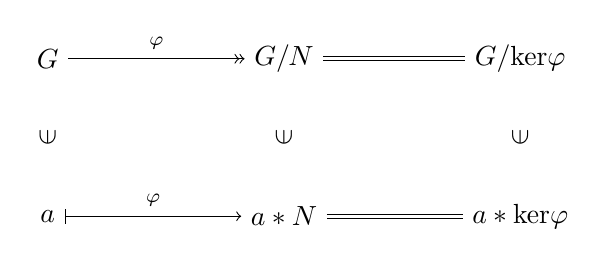
\begin{tikzpicture}[auto]
    \node[rotate=90] (a) at (0, 1) {$\in $};
    \node[rotate=90] (b) at (3, 1) {$\in $};
    \node[rotate=90] (c) at (6, 1) {$\in $};
    \node (a) at (0, 2) {$G$};
    \node (b) at (3, 2) {$G/N$};
    \node (c) at (6, 2) {$G/{\rm ker} \varphi $};
    \draw [->>] (a) to node {$\scriptstyle \varphi $} (b);
    \draw [double distance=1pt] (b) to node {$\scriptstyle $} (c);
    \node (a) at (0, 0) {$a$};
    \node (b) at (3, 0) {$a*N$};
    \node (c) at (6, 0) {$a*{\rm ker} \varphi $};
    \draw [|->] (a) to node {$\scriptstyle \varphi $} (b);
    \draw [double distance=1pt] (b) to node {$\scriptstyle $} (c);
  \end{tikzpicture}
\end{center}
\end{dfn}
\begin{proof}
群$(G,*)$の正規部分群$(N,*)$が与えられたとき、写像$\varphi:G \rightarrow G/N;a \mapsto a*N$について、$\forall a,b \in G$に対し、次のようになる。
\begin{align*}
\varphi(a*b) &= (a*b)*N\\
&= (a*b)*(N*N)\\
&= N*(a*b)*N\\
&= (a*N)*(b*N)\\
&= \varphi(a)*\varphi(b)
\end{align*}
これにより、その写像$\varphi$は群準同型写像である。\par
また、$\forall a*N$に対し、次のようになることから、
\begin{align*}
(a*N)*\left( 1_{(G,*)}*N \right) &= \varphi(a)*\varphi\left( 1_{(G,*)} \right)\\
&= \varphi\left( a*1_{(G,*)} \right)\\
&= \varphi(a) = a*N\\
&\left( 1_{(G,*)}*N \right)*(a*N) = \varphi\left( 1_{(G,*)} \right)*\varphi(a)\\
&= \varphi\left( 1_{(G,*)}*a \right)\\
&= \varphi(a) = a*N
\end{align*}
その群$(G/N,*)$の単位元は$1_{(G,*)}*N$である。したがって、$\forall a \in \ker\varphi$に対し、次のようになる。
\begin{align*}
\varphi(a) &= a*N\\
&= 1_{(G,*)}*N\\
&= N
\end{align*}
ここで、$\forall n \in N$に対し、$n = a*n'$なる元$n'$がその集合$N$に存在し次のようになるので、
\begin{align*}
a &= a*1_{(G,*)}\\
&= a*n'*{n'}^{- 1}\\
&= n*{n'}^{- 1} \in N
\end{align*}
$a \in N$が成り立つ。逆に、$\forall a \in N$が成り立つなら、次のようになるので、
\begin{align*}
\varphi(a) &= a*N\\
&= \left\{ a*n \in G \middle| n \in N \right\}\\
&= \left\{ a*n \in G \middle| a*n \in N \right\}\\
&= N
\end{align*}
$a \in \ker\varphi$が成り立つ。以上より、$\ker\varphi = N$が得られる。\par
最後に、$\forall a*N \in {G}/{N}$に対し、商群の定義より明らかに$\varphi(a) = a*N$なるその集合$G$の元$a$が存在するので、その写像$\varphi$は全射である。これにより、その写像$\varphi$は全射群準同型写像である。
\end{proof}
%\hypertarget{ux7fa4ux6e96ux540cux578bux5b9aux7406}{%
\subsubsection{群準同型定理}%\label{ux7fa4ux6e96ux540cux578bux5b9aux7406}}
\begin{thm}\label{3.1.2.8}
2つの群々$\left( G,*_{G} \right)$、$\left( H,*_{H} \right)$の間の群準同型写像$f:G \rightarrow H$について、$\forall a,b \in G$に対し、$f(a) = f(b)$が成り立つならそのときに限り、その群$\left( G,*_{G} \right)$の正規部分群$\left( \ker f,*_{G} \right)$を法としてその集合$G$の元々$a$、$b$が合同である、即ち、$a \equiv b\ \mathrm{mod}\left( \ker f,*_{G} \right)$が成り立つ。
\end{thm}
\begin{proof}
2つの群々$\left( G,*_{G} \right)$、$\left( H,*_{H} \right)$の間の群準同型写像$f:G \rightarrow H$について、$\forall a,b \in G$に対し、$f(a) = f(b)$が成り立つなら、その群準同型写像$f$の核$\ker f$を用いた組$\left( \ker f,*_{G} \right)$は定理\ref{3.1.2.6}よりその群$\left( G,*_{G} \right)$の正規部分群であり群準同型写像と核の定義より次のようになるので、
\begin{align*}
f\left( a^{- 1}*_{G}b \right) &= f\left( a^{- 1} \right)*_{H}f(b)\\
&= {f(a)}^{- 1}*_{H}f(b)\\
&= {f(b)}^{- 1}*_{H}f(b)\\
&= 1_{\left( H,*_{H} \right)}
\end{align*}
$a^{- 1}*_{G}b \in \ker f$が得られる。定理\ref{3.1.1.20}よりその正規部分群$\left( \ker f,*_{G} \right)$を法としてその集合$G$の元々$a$、$b$が合同である、即ち、$a \equiv b\ \mathrm{mod}\left( \ker f,*_{G} \right)$が成り立つ。
\end{proof}
\begin{thm}\label{3.1.2.9}
これの系として、2つの群々$\left( G,*_{G} \right)$、$\left( H,*_{H} \right)$の間の群準同型写像$f:G \rightarrow H$が単射であるならそのときに限り、その写像$f$の核$\ker f$が$\ker f = \left\{ 1_{\left( G,*_{G} \right)} \right\}$を満たす。
\end{thm}
\begin{proof}
2つの群々$\left( G,*_{G} \right)$、$\left( H,*_{H} \right)$の間の群準同型写像$f:G \rightarrow H$について、その群$\left( \left\{ 1_{\left( G,*_{G} \right)} \right\},*_{G} \right)$は、$1_{\left( G,*_{G} \right)} \in \left\{ 1_{\left( G,*_{G} \right)} \right\}$が成り立つかつ、$1_{\left( G,*_{G} \right)}*_{G}1_{\left( G,*_{G} \right)} \in \left\{ 1_{\left( G,*_{G} \right)} \right\}$が成り立つかつ、次のようになることから、
\begin{align*}
1_{\left( G,*_{G} \right)}^{- 1} &= 1_{\left( G,*_{G} \right)}^{- 1}*_{G}1_{\left( G,*_{G} \right)}\\
&= 1_{\left( G,*_{G} \right)}
\end{align*}
$1_{\left( G,*_{G} \right)}^{- 1} \in \left\{ 1_{\left( G,*_{G} \right)} \right\}$が成り立つので、定理\ref{3.1.1.6}よりその群$\left( G,*_{G} \right)$の部分群で、$\forall a \in G$に対し、次のようになるので、
\begin{align*}
1_{\left( G,*_{G} \right)} &= a*_{G}a^{- 1}\\
&= a*_{G}1_{\left( G,*_{G} \right)}*_{G}a^{- 1} \in \left\{ 1_{\left( G,*_{G} \right)} \right\}
\end{align*}
定理\ref{3.1.1.25}よりその群$\left( \left\{ 1_{\left( G,*_{G} \right)} \right\},*_{G} \right) \trianglelefteq \left( G,*_{G} \right)$が成り立つ。\par
その写像$f$の核$\ker f$が$\ker f = \left\{ 1_{\left( G,*_{G} \right)} \right\}$を満たすとき、2つの群々$\left( G,*_{G} \right)$、$\left( H,*_{H} \right)$の間の群準同型写像$f:G \rightarrow H$について、定理\ref{3.1.2.8}より次のようになる。
\begin{align*}
f(a) = f(b) &\Leftrightarrow a \equiv b\ \left( \mathrm{mod}\left\{ 1_{\left( G,*_{G} \right)} \right\} \right)\\
&\Leftrightarrow a^{- 1}*_{G}b \in \left\{ 1_{\left( G,*_{G} \right)} \right\}\\
&\Leftrightarrow a^{- 1}*_{G}b = 1_{\left( G,*_{G} \right)}\\
&\Leftrightarrow a*_{G}a^{- 1}*_{G}b = a*_{G}1_{\left( G,*_{G} \right)}\\
&\Leftrightarrow 1_{\left( G,*_{G} \right)}*_{G}b = a*_{G}1_{\left( G,*_{G} \right)}\\
&\Leftrightarrow a = b
\end{align*}
これにより、その写像$f$は単射である。\par
逆に、その写像$f$が単射であるなら、$\forall a,b \in G$に対し、次のようになる。
\begin{align*}
f(a) = f(b) &\Leftrightarrow a = b\\
&\Leftrightarrow a^{- 1}*_{G}a = a^{- 1}*_{G}b\\
&\Leftrightarrow a^{- 1}*_{G}b = 1_{\left( G,*_{G} \right)}\\
&\Leftrightarrow a^{- 1}*_{G}b \in \left\{ 1_{\left( G,*_{G} \right)} \right\}\\
&\Leftrightarrow a \equiv b\ \mathrm{mod}\left( \left\{ 1_{\left( G,*_{G} \right)} \right\},*_{G} \right)
\end{align*}
ここで、定理\ref{3.1.2.8}よりその写像$f$の核$\ker f$がその群$\left( G,*_{G} \right)$の単位元$1_{\left( G,*_{G} \right)}$のみからなる。
\end{proof}
\begin{thm}[群準同型定理]\label{3.1.2.10}
2つの群々$\left( G,*_{G} \right)$、$\left( H,*_{H} \right)$の間の群準同型写像$f:G \rightarrow H$について、写像$g:{G}/{\ker f} \rightarrow V(f);a*\ker f \mapsto f(a)$は群$\left( G/\ker f,*_{G} \right)$から群$\left( V(f),*_{H} \right)$への群同型写像でありこれらの2つの群々$\left( G/\ker f,*_{G} \right)$、$\left( V(f),*_{H} \right)$は群同型である、即ち、$\left( {G}/{\ker f},*_{G} \right) \cong \left( V(f),*_{H} \right)$が成り立つ。\par
この定理を群準同型定理という。この定理は、その群$\left( G,*_{G} \right)$からその商群$\left( {G}/{\ker f},*_{G} \right)$への自然な全射群準同型写像$\varphi$が用いられれば、次のように与えられる。
\begin{center}
  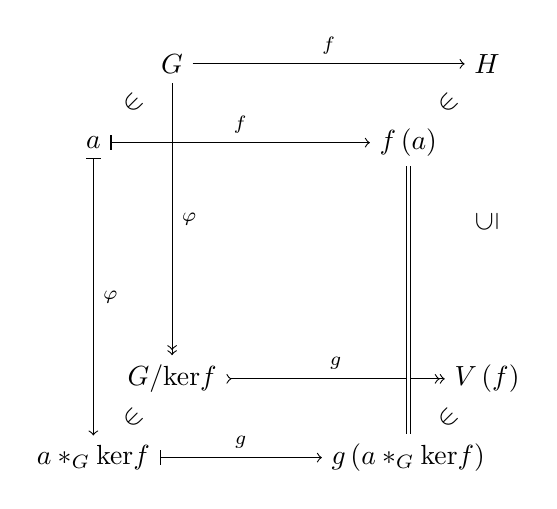
\begin{tikzpicture}[auto]
    \node (a) at (0, 0) {$a*_G {\rm ker} f$};
    \node (b) at (4, 0) {$g\left( a*_G {\rm ker} f\right) $};
    \node (c) at (0, 4) {$a$};
    \node (d) at (4, 4) {$f\left( a\right) $};
    \node (e) at (1, 1) {$G/{\rm ker} f$};
    \node (f) at (5, 1) {$V\left( f\right) $};
    \node (g) at (1, 5) {$G$};
    \node (h) at (5, 5) {$H$};
    \node[rotate=45] (i) at (0.5, 0.5) {$\in $};
    \node[rotate=45] (j) at (4.5, 0.5) {$\in $};
    \node[rotate=45] (k) at (0.5, 4.5) {$\in $};
    \node[rotate=45] (l) at (4.5, 4.5) {$\in $};
    \node[rotate=90] (m) at (5, 3) {$\subseteq $};
    \draw [|->] (a) to node {$\scriptstyle g$} (b);
    \draw [>->>] (e) to node {$\scriptstyle g$} (f);
    \draw [|->] (c) to node {$\scriptstyle \varphi $} (a);
    \draw [->>] (g) to node {$\scriptstyle \varphi $} (e);
    \draw [|->] (c) to node {$\scriptstyle f$} (d);
    \draw [->] (g) to node {$\scriptstyle f$} (h);
    \draw [double distance=1pt] (b) to node {$ $} (d);
  \end{tikzpicture} 
\end{center}
\end{thm}
\begin{proof}
2つの群々$\left( G,*_{G} \right)$、$\left( H,*_{H} \right)$の間の群準同型写像$f:G \rightarrow H$について、写像$g:{G}/{\ker f} \rightarrow V(f);a*_{G}\ker f \mapsto f(a)$が与えられるとき、$\forall a*_{G}\ker f,b*_{G}\ker f \in {G}/{\ker f}$に対し、$a*_{G}\ker f = b*_{G}\ker f$が成り立つなら、定理\ref{3.1.2.6}より$\left( \ker f,*_{G} \right) \trianglelefteq \left( G,*_{G} \right)$が成り立つので、$1_{\left( G,*_{G} \right)} \in \ker f$に注意すれば、$a*_{G}1_{\left( G,*_{G} \right)} \in a*_{G}\ker f = b*_{G}\ker f$が成り立つことにより、$\exists n \in \ker f$に対し、$a*_{G}1_{\left( G,*_{G} \right)} = b*_{G}n$が成り立つ。したがって、定理\ref{3.1.1.25}より次のようになる。
\begin{align*}
a*_{G}b^{- 1} &= a*_{G}1_{\left( G,*_{G} \right)}*_{G}b^{- 1}\\
&= b*_{G}n*_{G}b^{- 1} \in b*_{G}\ker f*_{G}b^{- 1} = \ker f
\end{align*}
ゆえに、次のようになる。
\begin{align*}
g\left( a*_{G}\ker f \right) &= f(a)\\
&= f(a)*_{H}1_{\left( H,*_{H} \right)}\\
&= f(a)*_{H}{f(b)}^{- 1}*_{H}f(b)\\
&= f(a)*_{H}f\left( b^{- 1} \right)*_{H}f(b)\\
&= f\left( a*_{G}b^{- 1} \right)*_{H}f(b)\\
&= 1_{\left( H,*_{H} \right)}*_{H}f(b)\\
&= f(b)\\
&= g\left( b*_{G}\ker f \right)
\end{align*}
ゆえに、その対応$g$は写像となっている。\par
その値域の定義より明らかにその写像$g$は全射である。また、$g\left( a*_{G}\ker f \right) = g\left( b*_{G}\ker f \right)$が成り立つなら、群$\left( \ker f,*_{G} \right)$はその群$\left( G,*_{G} \right)$の部分群であることにより次のようになる。
\begin{align*}
&\quad g\left( a*_{G}\ker f \right) = g\left( b*_{G}\ker f \right) \\
&\Leftrightarrow f(a) = f(b)\\
&\Leftrightarrow f(a)*_{H}{f(b)}^{- 1} = f(a)*_{H}f\left( b^{- 1} \right) = f\left( a*_{G}b^{- 1} \right) = 1_{\left( H,*_{H} \right)}\\
&\Leftrightarrow a*_{G}b^{- 1} \in \ker f\\
&\Leftrightarrow \left( a*_{G}b^{- 1} \right)^{- 1} = a^{- 1}*_{G}b \in \ker f
\end{align*}
ここで、定理\ref{3.1.1.18}よりその群$\left( G,*_{G} \right)$の部分群$\left( \ker f,*_{G} \right)$について、$a^{- 1}*_{G}b \in \ker f$が成り立つなら、$a*_{G}\ker f = b*_{G}\ker f$が成り立つのであったので、次のようになる。
\begin{align*}
g\left( a*_{G}\ker f \right) = g\left( b*_{G}\ker f \right) &\Leftrightarrow a^{- 1}*_{G}b \in \ker f\\
&\Rightarrow a*_{G}\ker f = b*_{G}\ker f
\end{align*}
したがって、その写像$g$は単射である。以上より、その写像$g$は全単射$g:{G}/{\ker f}\overset{\sim}{\rightarrow}V(f)$である。\par
その組$\left( \ker f,*_{G} \right)$はその群$\left( G,*_{G} \right)$の正規部分群であったので、$\forall a*_{G}\ker f,b*_{G}\ker f \in {G}/{\ker f}$に対し、次のようになる。
\begin{align*}
g\left( \left( a*_{G}\ker f \right)*_{G}\left( b*_{G}\ker f \right) \right) &= g\left( \ker f*_{G}a*_{G}b*_{G}\ker f \right)\\
&= g\left( \ker f*_{G}\left( a*_{G}b \right)*_{G}\ker f \right)\\
&= g\left( \left( a*_{G}b \right)*_{G}\ker f*_{G}\ker f \right)\\
&= g\left( \left( a*_{G}b \right)*_{G}\ker f \right)\\
&= f\left( a*_{G}b \right)\\
&= f(a)*_{H}f(b)\\
&= g\left( a*_{G}\ker f \right)*_{H}g\left( b*_{G}\ker f \right)
\end{align*}
これにより、その写像$g$は群準同型写像であり、その写像$g$は全単射だったので、その写像$g$は群同型写像である。\par
これにより、2つのそれらの群々$\left( G/\ker f,*_{G} \right)$、$\left( V(f),*_{H} \right)$は、その集合$G/\ker f$からその集合$V(f)$への群同型写像$g:{G}/{\ker f} \rightarrow V(f)$が存在するので、群同型である、即ち、$\left( {G}/{\ker f},*_{G} \right) \cong \left( V(f),*_{H} \right)$が成り立つ。\par
よって、その群$\left( G,*_{G} \right)$からその商群$\left( {G}/{\ker f},*_{G} \right)$への自然な全射群準同型写像$\varphi$が用いられれば、次のように与えられる。
\begin{center}
  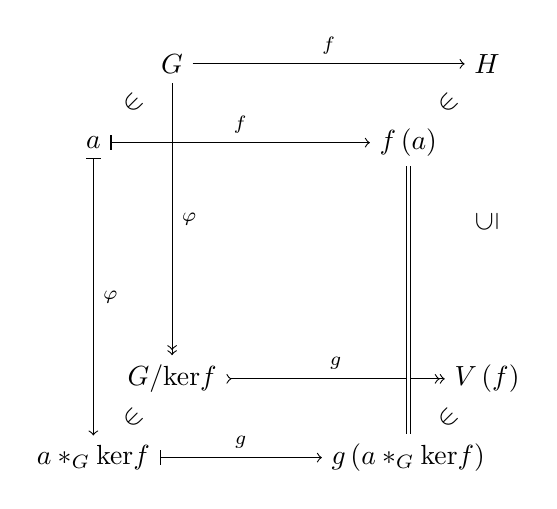
\begin{tikzpicture}[auto]
    \node (a) at (0, 0) {$a*_G {\rm ker} f$};
    \node (b) at (4, 0) {$g\left( a*_G {\rm ker} f\right) $};
    \node (c) at (0, 4) {$a$};
    \node (d) at (4, 4) {$f\left( a\right) $};
    \node (e) at (1, 1) {$G/{\rm ker} f$};
    \node (f) at (5, 1) {$V\left( f\right) $};
    \node (g) at (1, 5) {$G$};
    \node (h) at (5, 5) {$H$};
    \node[rotate=45] (i) at (0.5, 0.5) {$\in $};
    \node[rotate=45] (j) at (4.5, 0.5) {$\in $};
    \node[rotate=45] (k) at (0.5, 4.5) {$\in $};
    \node[rotate=45] (l) at (4.5, 4.5) {$\in $};
    \node[rotate=90] (m) at (5, 3) {$\subseteq $};
    \draw [|->] (a) to node {$\scriptstyle g$} (b);
    \draw [>->>] (e) to node {$\scriptstyle g$} (f);
    \draw [|->] (c) to node {$\scriptstyle \varphi $} (a);
    \draw [->>] (g) to node {$\scriptstyle \varphi $} (e);
    \draw [|->] (c) to node {$\scriptstyle f$} (d);
    \draw [->] (g) to node {$\scriptstyle f$} (h);
    \draw [double distance=1pt] (b) to node {$ $} (d);
  \end{tikzpicture} 
\end{center}
\end{proof}
\begin{dfn}
2つの群々$\left( G,*_{G} \right)$、$\left( H,*_{H} \right)$の間のある全射群準同型写像$f:G \twoheadrightarrow H$が存在するとき、その群$\left( H,*_{H} \right)$はその群$\left( G,*_{G} \right)$の群準同型像という。
\end{dfn}
\begin{thm}\label{3.1.2.11}
群$\left( H,*_{H} \right)$が群$\left( G,*_{G} \right)$の群準同型像であるならそのときに限り、その群$\left( H,*_{H} \right)$と群同型であるようなその群$\left( G,*_{G} \right)$のある商群が存在する。
\end{thm}
\begin{proof}
定義より群$\left( H,*_{H} \right)$が群$\left( G,*_{G} \right)$の群準同型像であるならそのときに限り、それらの群々$\left( G,*_{G} \right)$、$\left( H,*_{H} \right)$の間の全射群準同型写像$f:G \twoheadrightarrow H$が存在するのであった。このとき、群準同型定理と$V(f) = H$が成り立つことより写像$g:G/\ker f\overset{\sim}{\rightarrow}H$は群同型写像でありそれらの群々$\left( {G}/{\ker f},*_{G} \right)$、$\left( H,*_{H} \right)$は群同型である。したがって、その群$\left( H,*_{H} \right)$と群同型であるようなその群$\left( G,*_{G} \right)$のある商群が存在する。\par
逆に、その群$\left( H,*_{H} \right)$と群同型であるようなその群$\left( G,*_{G} \right)$のある商群が存在するなら、その群$\left( G,*_{G} \right)$のある正規部分群$\left( N,*_{G} \right)$を用いてその商群が$\left( {G}/{N},*_{G} \right)$とおかれれば、群同型写像$g:{G}/{N}\overset{\sim}{\rightarrow}H$が存在できる。また、写像$\varphi:G \rightarrow {G}/{N};a \mapsto a*_{G}N$は定理\ref{3.1.2.7}より全射群準同型写像で$\ker\varphi = N$が成り立つのであったので、次式のような写像$g \circ \varphi$を考えると、
\begin{center}
  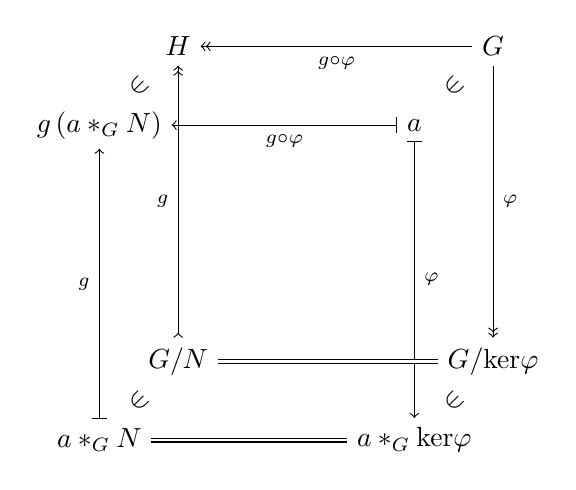
\begin{tikzpicture}[auto]
    \node[rotate=45] (x) at (7.5, 0.5) {$\in $};
    \node[rotate=45] (x) at (7.5, 4.5) {$\in $};
    \node[rotate=45] (x) at (3.5, 0.5) {$\in $};
    \node[rotate=45] (x) at (3.5, 4.5) {$\in $};
    \node (a) at (7, 0) {$a*_G {\rm ker} \varphi $};
    \node (c) at (7, 4) {$a$};
    \node (e) at (8, 1) {$G/{\rm ker} \varphi $};
    \node (g) at (8, 5) {$G$};
    \node (i) at (3, 0) {$a*_G N$};
    \node (j) at (3, 4) {$g\left( a*_G N\right) $};
    \node (k) at (4, 1) {$G/N$};
    \node (l) at (4, 5) {$H$};
    \draw [|->] (c) to node {$\scriptstyle \varphi $} (a);
    \draw [->>] (g) to node {$\scriptstyle \varphi $} (e);
    \draw [double distance=1pt] (a) to node {} (i);
    \draw [double distance=1pt] (e) to node {} (k);
    \draw [|->] (i) to node {$\scriptstyle g$} (j);
    \draw [>->>] (k) to node {$\scriptstyle g$} (l);
    \draw [|->] (c) to node {$\scriptstyle g\circ \varphi $} (j);
    \draw [->>] (g) to node {$\scriptstyle g\circ \varphi $} (l);
  \end{tikzpicture} 
\end{center}
これは全射群準同型写像$g \circ \varphi:G \twoheadrightarrow H$であるので、その群$\left( H,*_{H} \right)$はその群$\left( G,*_{G} \right)$の群準同型像である。
\end{proof}
%\hypertarget{ux7fa4ux540cux578bux5b9aux7406}{%
\subsubsection{群同型定理}%\label{ux7fa4ux540cux578bux5b9aux7406}}
\begin{thm}\label{3.1.2.12}
2つの群々$\left( G,*_{G} \right)$、$\left( H,*_{H} \right)$の間の全射群準同型写像$f:G \twoheadrightarrow H$について、その群$\left( G,*_{G} \right)$の部分群$\left( I,*_{G} \right)$と正規部分群$\left( M,*_{G} \right)$を用いた2つの組々$\left( V\left( f|I \right),*_{H} \right)$、$\left( V\left( f|M \right),*_{H} \right)$はそれぞれその群$\left( H,*_{H} \right)$の部分群、正規部分群である。\par
また、その群$\left( H,*_{H} \right)$の部分群$\left( J,*_{H} \right)$と正規部分群$\left( N,*_{H} \right)$を用いた2つの組々$\left( V\left( f^{- 1}|J \right),*_{G} \right)$、$\left( V\left( f^{- 1}|N \right),*_{G} \right)$はそれぞれその群$\left( G,*_{G} \right)$の部分群、正規部分群である。
\end{thm}
\begin{proof}
2つの群々$\left( G,*_{G} \right)$、$\left( H,*_{H} \right)$の間の全射群準同型写像$f:G \twoheadrightarrow H$について、その群$\left( G,*_{G} \right)$の部分群$\left( I,*_{G} \right)$と正規部分群$\left( M,*_{G} \right)$を用いた2つの組々$\left( V\left( f|I \right),*_{H} \right)$、$\left( V\left( f|M \right),*_{H} \right)$が与えられたとする。$f|I(a),f|I(b) \in V\left( f|I \right)$のとき、定理\ref{3.1.1.6}より$a,b \in I$が成り立つなら、$a*_{G}b \in I$も成り立つので、次のようになる。
\begin{align*}
f|I(a)*_{H}f|I(b) = f|I\left( a*_{G}b \right) \in V\left( f|I \right)
\end{align*}
$f|I\left( a^{- 1} \right) = {f|I(a)}^{- 1}$が成り立つことと定理\ref{3.1.1.6}より$a \in I$が成り立つなら、$a^{- 1} \in I$も成り立つので、次のようになる。
\begin{align*}
{f|I(a)}^{- 1} = f|I\left( a^{- 1} \right) \in V\left( f|I \right)
\end{align*}
したがって、組$\left( V\left( f|I \right),*_{H} \right)$は定理\ref{3.1.1.6}よりその群$\left( H,*_{H} \right)$の部分群である。\par
同様にして、群$\left( V\left( f|M \right),*_{H} \right)$はその群$\left( H,*_{H} \right)$の部分群であることが示され、$f|M\left( a^{- 1} \right) =$
${f|M(a)}^{- 1}$が成り立つことと定理\ref{3.1.1.25}より$h \in M$が成り立つなら、$\forall b \in G$に対し、$b*_{G}h*_{G}b^{- 1} \in M$も成り立つので、次のようになる。
\begin{align*}
f(b)*_{H}f|M(a)*_{H}{f(b)}^{- 1} &= f(b)*_{H}f(a)*_{H}f\left( b^{- 1} \right)\\
&= f\left( b*_{G}h*_{G}b^{- 1} \right) \in V\left( f|M \right)
\end{align*}
したがって、組$\left( V\left( f|M \right),*_{H} \right)$は定理\ref{3.1.1.25}よりその群$\left( H,*_{H} \right)$の正規部分群である。\par
また、その群$\left( H,*_{H} \right)$の部分群$\left( J,*_{H} \right)$と正規部分群$\left( N,*_{H} \right)$を用いた2つの集合たち$V\left( f^{- 1}|J \right)$、$V\left( f^{- 1}|N \right)$が与えられたとする。群準同型写像の定義と定理\ref{3.1.1.6}より$a,b \in J$が成り立つなら、$a*_{H}b \in J$も成り立つので、次のようになる。
\begin{align*}
a,b \in V\left( f^{- 1}|J \right) &\Rightarrow f(a),f(b) \in V\left( f|V\left( f^{- 1}|J \right) \right) \subseteq J\\
&\Rightarrow f(a)*_{H}f(b) = f\left( a*_{H}b \right) \in J\\
&\Rightarrow a*_{G}b \in V\left( f^{- 1}|J \right)
\end{align*}
$f\left( a^{- 1} \right) = {f(a)}^{- 1}$が成り立つことと定理\ref{3.1.1.6}より$a \in J$が成り立つなら、$a^{- 1} \in J$も成り立つので、次のようになる。
\begin{align*}
a \in V\left( f^{- 1}|J \right) &\Rightarrow f(a) \in V\left( f|V\left( f^{- 1}|J \right) \right) \subseteq J\\
&\Rightarrow {f(a)}^{- 1} = f\left( a^{- 1} \right) \in J\\
&\Rightarrow a^{- 1} \in V\left( f^{- 1}|J \right)
\end{align*}
したがって、組$\left( V\left( f^{- 1}|J \right),*_{G} \right)$はその群$\left( G,*_{G} \right)$の部分群である。\par
同様にして、組$\left( V\left( f^{- 1}|N \right),*_{G} \right)$はその群$\left( G,*_{G} \right)$の部分群であることが示され群準同型写像の定義と${f(a)}^{- 1} = f\left( a^{- 1} \right)$が成り立つことと正規部分群の定義より次のようになる。
\begin{align*}
b \in a*_{G}V\left( f^{- 1}|N \right) &\Leftrightarrow a^{- 1}*_{G}b \in a^{- 1}*_{G}a*_{G}V\left( f^{- 1}|N \right) = 1_{\left( G,*_{G} \right)}*_{G}V\left( f^{- 1}|N \right) = V\left( f^{- 1}|N \right)\\
&\Leftrightarrow f\left( a^{- 1}*_{G}b \right) \in V\left( f|V\left( f^{- 1}|N \right) \right) \subseteq N\\
&\Rightarrow f\left( a^{- 1} \right)*_{H}f(b) = {f(a)}^{- 1}*_{H}f(b) \in N\\
&\Leftrightarrow f(a)*_{H}{f(a)}^{- 1}*_{H}f(b) = 1_{\left( H,*_{H} \right)}*_{H}f(b) = f(b) \in f(a)*_{H}N\\
&\Leftrightarrow f(b) \in f(a)*_{H}N = N*_{H}f(a)\\
&\Leftrightarrow f(b)*_{H}{f(a)}^{- 1} \in N*_{H}f(a)*_{H}{f(a)}^{- 1} = N*_{H}1_{\left( H,*_{H} \right)} = N\\
&\Leftrightarrow f(b)*_{H}{f(a)}^{- 1} = f(b)*_{H}f\left( a^{- 1} \right) = f\left( b*_{G}a^{- 1} \right) \in N\\
&\Leftrightarrow b*_{G}a^{- 1} \in V\left( f^{- 1}|N \right)\\
&\Leftrightarrow b*_{G}a^{- 1}*_{G}a = b*_{G}1_{\left( G,*_{G} \right)} = b \in V\left( f^{- 1}|N \right)*_{G}a
\end{align*}
これにより、$a*_{G}V\left( f^{- 1}|N \right) \subseteq V\left( f^{- 1}|N \right)*_{G}a$が成り立つ。同様にして、$a*_{G}V\left( f^{- 1}|N \right) \supseteq V\left( f^{- 1}|N \right)*_{G}a$も成り立つことが示されるので、$a*_{G}V\left( f^{- 1}|N \right) = V\left( f^{- 1}|N \right)*_{G}a$が成り立ち、したがって、組$\left( V\left( f^{- 1}|N \right),*_{G} \right)$はその群$\left( G,*_{G} \right)$の正規部分群である。
\end{proof}
\begin{thm}[第1群同型定理]\label{3.1.2.13}
2つの群々$\left( G,*_{G} \right)$、$\left( H,*_{H} \right)$の間の全射群準同型写像$f:G \twoheadrightarrow H$について、その群$\left( G,*_{G} \right)$の部分群をなす$\ker f \subseteq I$が成り立つようなその集合$G$の部分集合全体の集合を$\varOmega_{\left( G,*_{G} \right)}'$、その群$\left( H,*_{H} \right)$の部分群をなすその集合$H$の部分集合全体の集合を$\varOmega_{\left( H,*_{H} \right)}$とおくと、次のことが成り立つ。
\begin{itemize}
\item
  次式のように写像$F:\varOmega_{\left( G,*_{G} \right)}' \rightarrow \varOmega_{\left( H,*_{H} \right)};I \mapsto V\left( f|I \right)$は全単射でその逆写像$F^{- 1}$が$F^{- 1}:\varOmega_{\left( H,*_{H} \right)} \rightarrow \varOmega_{\left( G,*_{G} \right)}';J \mapsto V\left( f^{- 1}|J \right)$と与えられる。
  \begin{center}
    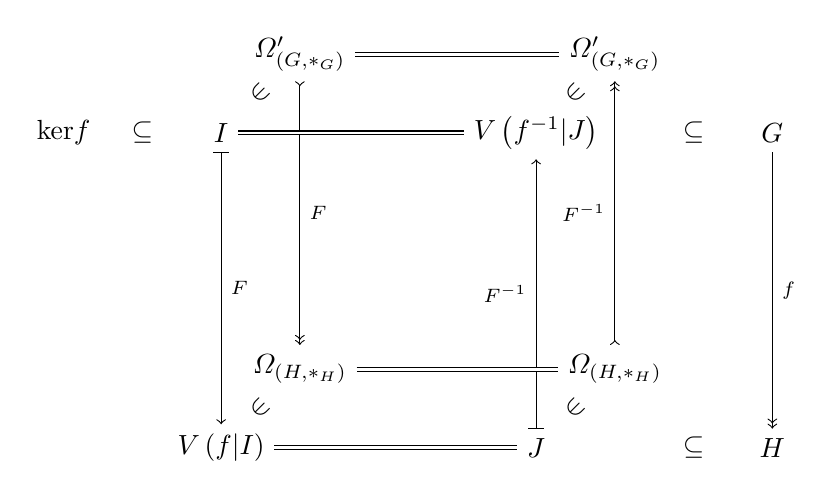
\begin{tikzpicture}[auto]
      \node[rotate=45] (x) at (2.5, 4.5) {$\in $};
      \node[rotate=45] (x) at (2.5, 0.5) {$\in $};
      \node[rotate=45] (x) at (6.5, 0.5) {$\in $};
      \node[rotate=45] (x) at (6.5, 4.5) {$\in $};
      \node (y) at (1, 4) {$\subseteq $};
      \node (y) at (8, 4) {$\subseteq $};
      \node (y) at (8, 0) {$\subseteq $};
      \node (a) at (3, 5) {$\varOmega_{\left(G,*_G \right)}' $};
      \node (b) at (3, 1) {$\varOmega_{\left(H,*_H \right)} $};
      \node (c) at (2, 4) {$I$};
      \node (d) at (2, 0) {$V\left( f|I\right) $};
      \node (e) at (6, 0) {$J$};
      \node (f) at (6, 4) {$V\left( f^{-1} |J\right) $};
      \node (g) at (7, 1) {$\varOmega_{\left(H,*_H \right)} $};
      \node (h) at (7, 5) {$\varOmega_{\left(G,*_G \right)}' $};
      \node (i) at (9, 4) {$G$};
      \node (j) at (9, 0) {$H$};
      \node (k) at (0, 4) {${\rm ker} f$};
      \draw [>->>] (a) to node {$\scriptstyle F$} (b);
      \draw [|->] (c) to node {$\scriptstyle F$} (d);
      \draw [>->>] (g) to node {$\scriptstyle F^{-1} $} (h);
      \draw [|->] (e) to node {$\scriptstyle F^{-1} $} (f);
      \draw [->>] (i) to node {$\scriptstyle f$} (j);
      \draw [double distance=1pt] (c) to node {} (f);
      \draw [double distance=1pt] (d) to node {} (e);
      \draw [double distance=1pt] (a) to node {} (h);
      \draw [double distance=1pt] (b) to node {} (g);
    \end{tikzpicture} 
  \end{center}
\item
  $\forall I \in \varOmega_{\left( G,*_{G} \right)}'$に対し、$\left( {I}/{\ker f},*_{G} \right) \cong \left( F(I),*_{H} \right)$が成り立つ。これは次式のようにも表される。
  \begin{center}
    \begin{tikzpicture}[auto]
      \node[rotate=45] (x) at (2.5, 4.5) {$\in $};
      \node[rotate=45] (x) at (2.5, 0.5) {$\in $};
      \node (y) at (1, 4) {$\subseteq $};
      \node (y) at (7, 4) {$\subseteq $};
      \node (y) at (7, 0) {$\subseteq $};
      \node (a) at (3, 5) {$\varOmega_{\left(G,*_G \right)}' $};
      \node (b) at (3, 1) {$\varOmega_{\left(H,*_H \right)} $};
      \node (c) at (2, 4) {$I$};
      \node (d) at (2, 0) {$V\left( f|I\right) $};
      \node (e) at (6, 0) {$J$};
      \node (f) at (12, 4) {$I/{\rm ker} f$};
      \node (i) at (8, 4) {$G$};
      \node (j) at (8, 0) {$H$};
      \node (k) at (0, 4) {${\rm ker} f$};
      \draw [>->>] (a) to node {$\scriptstyle F$} (b);
      \draw [|->] (c) to node {$\scriptstyle F$} (d);
      \draw [>->>] (f) to node {} (e);
      \draw [->>] (i) to node {$\scriptstyle f$} (j);
      \draw [double distance=1pt] (d) to node {} (e);
      \draw [->>] (c)[bend left=10] to node {} (f);
    \end{tikzpicture} 
  \end{center}
\end{itemize}
\begin{itemize}
\item
  $\forall I \in \varOmega_{\left( G,*_{G} \right)}'$に対し、その写像$F:\varOmega_{\left( G,*_{G} \right)}' \rightarrow \varOmega_{\left( H,*_{H} \right)};I \mapsto V\left( f|I \right)$が与えられたとき、$\left( I,*_{G} \right) \trianglelefteq \left( G,*_{G} \right)$が成り立つならそのときに限り、$\left( F(I),*_{H} \right) \trianglelefteq \left( H,*_{H} \right)$が成り立つ。
\item
  $\forall I \in \varOmega_{\left( G,*_{G} \right)}'$に対し、上記の写像$F:\varOmega_{\left( G,*_{G} \right)}' \rightarrow \varOmega_{\left( H,*_{H} \right)};I \mapsto V\left( f|I \right)$が与えられたとき、$\left( I,*_{G} \right) \trianglelefteq \left( G,*_{G} \right)$が成り立つなら、$\left( G/I,*_{G} \right) \cong \left( H/F(I),*_{H} \right)$が成り立つ。これは次式のようにも表される。
  \begin{center}
    \begin{tikzpicture}[auto]
      \node[rotate=45] (x) at (2.5, 4.5) {$\in $};
      \node[rotate=45] (x) at (2.5, 0.5) {$\in $};
      \node (y) at (1, 4) {$\subseteq $};
      \node (y) at (7, 4) {$\subseteq $};
      \node (y) at (7, 0) {$\subseteq $};
      \node (a) at (3, 5) {$\varOmega_{\left(G,*_G \right)}' $};
      \node (b) at (3, 1) {$\varOmega_{\left(H,*_H \right)} $};
      \node (c) at (2, 4) {$I$};
      \node (d) at (2, 0) {$V\left( f|I\right) $};
      \node (e) at (6, 0) {$J$};
      \node (g) at (12, 0) {$H/J$};
      \node (h) at (12, 4) {$G/I$};
      \node (i) at (8, 4) {$G$};
      \node (j) at (8, 0) {$H$};
      \node (k) at (0, 4) {${\rm ker} f$};
      \draw [>->>] (a) to node {$\scriptstyle F$} (b);
      \draw [|->] (c) to node {$\scriptstyle F$} (d);
      \draw [>->>] (h) to node {} (g);
      \draw [->>] (i) to node {$\scriptstyle f$} (j);
      \draw [double distance=1pt] (d) to node {} (e);
      \draw [->>] (i) to node {} (h);
      \draw [->>] (j) to node {} (g);
    \end{tikzpicture} 
  \end{center}
\end{itemize}\par
この定理を第1群同型定理という。
\end{thm}
\begin{proof}
2つの群々$\left( G,*_{G} \right)$、$\left( H,*_{H} \right)$の間の全射群準同型写像$f:G \twoheadrightarrow H$について、その群$\left( G,*_{G} \right)$の部分群をなすその集合$G$のその核$\ker f$を含む部分集合全体の集合を$\varOmega_{\left( G,*_{G} \right)}'$、その群$\left( H,*_{H} \right)$の部分群をなすその集合$H$の部分集合全体の集合を$\varOmega_{\left( H,*_{H} \right)}$とおく。次式のように写像$F:\varOmega_{\left( G,*_{G} \right)}' \rightarrow \varOmega_{\left( H,*_{H} \right)};I \mapsto V\left( f|I \right) = J$を考えよう。
\begin{center}
  \begin{tikzpicture}[auto]
    \node[rotate=45] (x) at (2.5, 4.5) {$\in $};
    \node[rotate=45] (x) at (2.5, 0.5) {$\in $};
    \node (y) at (1, 4) {$\subseteq $};
    \node (y) at (7, 4) {$\subseteq $};
    \node (y) at (7, 0) {$\subseteq $};
    \node (a) at (3, 5) {$\varOmega_{\left(G,*_G \right)}' $};
    \node (b) at (3, 1) {$\varOmega_{\left(H,*_H \right)} $};
    \node (c) at (2, 4) {$I$};
    \node (d) at (2, 0) {$V\left( f|I\right) $};
    \node (e) at (6, 0) {$J$};
    \node (i) at (8, 4) {$G$};
    \node (j) at (8, 0) {$H$};
    \node (k) at (0, 4) {${\rm ker} f$};
    \draw [->] (a) to node {$\scriptstyle F$} (b);
    \draw [|->] (c) to node {$\scriptstyle F$} (d);
    \draw [->>] (i) to node {$\scriptstyle f$} (j);
    \draw [double distance=1pt] (d) to node {} (e);
  \end{tikzpicture} 
\end{center}
$\forall I \in \varOmega_{\left( G,*_{G} \right)}'$に対し、$V\left( f|I \right) = J$とおくと、定理\ref{3.1.2.12}よりその群$\left( G,*_{G} \right)$の部分群$\left( I,*_{G} \right)$を用いた組$\left( J,*_{H} \right)$はその群$\left( H,*_{H} \right)$の部分群であったので、$F(I) = V\left( f|I \right) \in \varOmega_{\left( H,*_{H} \right)}$が成り立つ。したがって、写像$F:\varOmega_{\left( G,*_{G} \right)}' \rightarrow \varOmega_{\left( H,*_{H} \right)};I \mapsto V\left( f|I \right)$が定義できている。ここで、次式のように写像$E:\varOmega_{\left( H,*_{H} \right)} \rightarrow \varOmega_{\left( G,*_{G} \right)}';J \mapsto V\left( f^{- 1}|J \right) = I$を考えよう。
\begin{center}
  \begin{tikzpicture}[auto]
    \node[rotate=45] (x) at (2.5, 4.5) {$\in $};
    \node[rotate=45] (x) at (2.5, 0.5) {$\in $};
    \node[rotate=45] (x) at (6.5, 0.5) {$\in $};
    \node[rotate=45] (x) at (6.5, 4.5) {$\in $};
    \node (y) at (1, 4) {$\subseteq $};
    \node (y) at (8, 4) {$\subseteq $};
    \node (y) at (8, 0) {$\subseteq $};
    \node (a) at (3, 5) {$\varOmega_{\left(G,*_G \right)}' $};
    \node (b) at (3, 1) {$\varOmega_{\left(H,*_H \right)} $};
    \node (c) at (2, 4) {$I$};
    \node (d) at (2, 0) {$V\left( f|I\right) $};
    \node (e) at (6, 0) {$J$};
    \node (f) at (6, 4) {$V\left( f^{-1} |J\right) $};
    \node (g) at (7, 1) {$\varOmega_{\left(H,*_H \right)} $};
    \node (h) at (7, 5) {$\varOmega_{\left(G,*_G \right)}' $};
    \node (i) at (9, 4) {$G$};
    \node (j) at (9, 0) {$H$};
    \node (k) at (0, 4) {${\rm ker} f$};
    \draw [->] (a) to node {$\scriptstyle F$} (b);
    \draw [|->] (c) to node {$\scriptstyle F$} (d);
    \draw [->] (g) to node {$\scriptstyle E$} (h);
    \draw [|->] (e) to node {$\scriptstyle E$} (f);
    \draw [->>] (i) to node {$\scriptstyle f$} (j);
    \draw [double distance=1pt] (d) to node {} (e);
    \draw [double distance=1pt] (a) to node {} (h);
    \draw [double distance=1pt] (b) to node {} (g);
  \end{tikzpicture} 
\end{center}
$\forall J \in \varOmega_{\left( H,*_{H} \right)}$に対し、$V\left( f^{- 1}|J \right) = I$とおくと、$\left\{ 1_{\left( H,*_{H} \right)} \right\} \subseteq J$が成り立つことから、$\ker f = V\left( f^{- 1}|\left\{ 1_{\left( H,*_{H} \right)} \right\} \right) \subseteq V\left( f^{- 1}|J \right) = I$が成り立つかつ、定理\ref{3.1.2.12}よりその群$\left( H,*_{H} \right)$の部分群$\left( J,*_{H} \right)$を用いた組$\left( I,*_{G} \right)$はその群$\left( G,*_{G} \right)$の部分群であったので、$E(J) = V\left( f^{- 1}|J \right) \in \varOmega_{\left( G,*_{G} \right)}'$が成り立つ。したがって、写像$E:\varOmega_{\left( H,*_{H} \right)} \rightarrow \varOmega_{\left( G,*_{G} \right)}';J \mapsto V\left( f^{- 1}|J \right)$が考えられることができる。\par
まず、$E \circ F = I_{\varOmega_{\left( G,*_{G} \right)}'}$が成り立つことを示そう。このとき、$\forall I \in \varOmega_{\left( G,*_{G} \right)}'$に対し、$V\left( f^{- 1}|V\left( f|I \right) \right) \supseteq I$は明らかに成り立つ。逆に、$\forall a \in G$に対し、$a \in V\left( f^{- 1}|V\left( f|I \right) \right)$が成り立つなら、$V\left( f|V\left( f^{- 1}|V\left( f|I \right) \right) \right) \subseteq V\left( f|I \right)$が成り立つので、$f(a) \in V\left( f|V\left( f^{- 1}|V\left( f|I \right) \right) \right) \subseteq V\left( f|I \right)$が成り立ち、したがって、$f(a) = f(b)$なるその集合$I$の元$b$が存在する。ここで、定理\ref{3.1.2.8}よりこれが成り立つならそのときに限り、$a \equiv b\ \mathrm{mod}\left( \ker f,*_{G} \right)$が成り立つのであったので、$a*_{G}b^{- 1} \in \ker f$が成り立ち、その集合$\varOmega_{\left( G,*_{G} \right)}'$の定義より、$a*_{G}b^{- 1} \in I$が成り立つ。したがって、$b \in I$が成り立つことと定理\ref{3.1.1.6}より次のようになる。
\begin{align*}
\left( a*_{G}b^{- 1} \right)*_{G}b &= a*_{G}\left( b^{- 1}*_{G}b \right)\\
&= a*_{G}1_{\left( G,*_{G} \right)}\\
&= a \in I
\end{align*}
以上より、$a \in I$が成り立つので、$V\left( f^{- 1}|V\left( f|I \right) \right) \subseteq I$が成り立つ。したがって、$V\left( f^{- 1}|V\left( f|I \right) \right) = I$が成り立つので、$E \circ F(I) = I$が成り立つ。\par
次に、$F \circ G = I_{\varOmega_{\left( H,*_{H} \right)}}$が成り立つことを示そう。$\forall J \in \varOmega_{\left( H,*_{H} \right)}$に対し、その対応$f$は写像なので、もちろん、$V\left( f|V\left( f^{- 1}|J \right) \right) = J$は成り立つ。したがって、$F \circ G(J) = V\left( f|V\left( f^{- 1}|J \right) \right) = J$が成り立つ。\par
以上より、$E \circ F = I_{\varOmega_{\left( G,*_{G} \right)}'}$かつ$F \circ G = I_{\varOmega_{\left( H,*_{H} \right)}}$が成り立つので、その写像$F:\varOmega_{\left( G,*_{G} \right)}' \rightarrow \varOmega_{\left( H,*_{H} \right)}$は全単射でその写像$E$がその写像$F$の逆写像である。よって、次式のように写像$F:\varOmega_{\left( G,*_{G} \right)}' \rightarrow \varOmega_{\left( H,*_{H} \right)};I \mapsto V\left( f|I \right)$は全単射でその逆写像$F^{- 1}$が$F^{- 1}:\varOmega_{\left( H,*_{H} \right)} \rightarrow \varOmega_{\left( G,*_{G} \right)}';J \mapsto V\left( f^{- 1}|J \right)$と与えられる。\par
また、$\forall I \in \varOmega_{\left( G,*_{G} \right)}'$に対し、$F(I) = V\left( f|I \right) = J$とおくと、写像$f':I \rightarrow J;a \mapsto f(a)$は明らかに全射群準同型写像であるから、次式のように考えられると、
\begin{center}
  \begin{tikzpicture}[auto]
    \node[rotate=45] (x) at (2.5, 4.5) {$\in $};
    \node[rotate=45] (x) at (2.5, 0.5) {$\in $};
    \node[rotate=45] (x) at (6.5, 4.5) {$\in $};
    \node (a) at (3, 5) {$I$};
    \node (b) at (3, 1) {$I/{\rm ker} f' $};
    \node (c) at (2, 4) {$a$};
    \node (d) at (2, 0) {$a*_G {\rm ker} f' $};
    \node (f) at (6, 4) {$f\left( a\right) $};
    \node (g) at (7, 1) {$V\left( f'|I\right) $};
    \node (h) at (7, 5) {$J$};
    \draw [->>] (a) to node {} (b);
    \draw [|->] (c) to node {} (d);
    \draw [->>] (a) to node {$\scriptstyle f'$} (h);
    \draw [|->] (c) to node {$\scriptstyle f'$} (f);
    \draw [double distance=1pt] (g) to node {} (h);
  \end{tikzpicture} 
\end{center}
群準同型定理より次式が成り立つので、
\begin{center}
  \begin{tikzpicture}[auto]
    \node[rotate=45] (x) at (2.5, 4.5) {$\in $};
    \node[rotate=45] (x) at (2.5, 0.5) {$\in $};
    \node[rotate=45] (x) at (6.5, 4.5) {$\in $};
    \node (a) at (3, 5) {$I$};
    \node (b) at (3, 1) {$I/{\rm ker} f' $};
    \node (c) at (2, 4) {$a$};
    \node (d) at (2, 0) {$a*_G {\rm ker} f' $};
    \node (f) at (6, 4) {$f\left( a\right) $};
    \node (g) at (7, 1) {$V\left( f'|I\right) $};
    \node (h) at (7, 5) {$J$};
    \draw [->>] (a) to node {} (b);
    \draw [|->] (c) to node {} (d);
    \draw [->>] (a) to node {$\scriptstyle f'$} (h);
    \draw [|->] (c) to node {$\scriptstyle f'$} (f);
    \draw [double distance=1pt] (g) to node {} (h);
    \draw [>->>] (b) to node {} (g);
  \end{tikzpicture} 
\end{center}
$\left( {I}/{\ker f'},*_{G} \right) \cong \left( V\left( f'|I \right),*_{H} \right)$が得られる。$\ker f \subseteq I$より$V\left( f'|I \right) = V\left( f|I \right) = J$が成り立つかつ、$\ker f' = \ker f$が成り立つので、$\left( {I}/{\ker f},*_{G} \right) \cong \left( J,*_{H} \right)$が成り立つ。\par
$\forall I \in \varOmega_{\left( G,*_{G} \right)}'$に対し、その写像$F:\varOmega_{\left( G,*_{G} \right)}' \rightarrow \varOmega_{\left( H,*_{H} \right)};I \mapsto V\left( f|I \right)$が与えられたとき、定理\ref{3.1.2.12}より$\left( I,*_{G} \right) \trianglelefteq \left( G,*_{G} \right)$が成り立つならそのときに限り、$\left( F(I),*_{H} \right) \trianglelefteq \left( H,*_{H} \right)$が成り立つことが直ちに分かる。\par
$\forall I \in \varOmega_{\left( G,*_{G} \right)}'$に対し、上記の写像$F:\varOmega_{\left( G,*_{G} \right)}' \rightarrow \varOmega_{\left( H,*_{H} \right)};I \mapsto V\left( f|I \right)$が与えられたとき、$\left( I,*_{G} \right) \trianglelefteq \left( G,*_{G} \right)$が成り立つなら、$F(I) = V\left( f|I \right) = J$とおいて次式のように自然な全射群準同型写像$\varphi_{H}:H \twoheadrightarrow H/J$を考えると、
\begin{center}
  \begin{tikzpicture}[auto]
    \node[rotate=45] (x) at (2.5, 4.5) {$\in $};
    \node[rotate=45] (x) at (2.5, 0.5) {$\in $};
    \node (y) at (1, 4) {$\subseteq $};
    \node (y) at (7, 4) {$\subseteq $};
    \node (y) at (7, 0) {$\subseteq $};
    \node (a) at (3, 5) {$\varOmega_{\left(G,*_G \right)}' $};
    \node (b) at (3, 1) {$\varOmega_{\left(H,*_H \right)} $};
    \node (c) at (2, 4) {$I$};
    \node (d) at (2, 0) {$V\left( f|I\right) $};
    \node (e) at (6, 0) {$J$};
    \node (g) at (12, 0) {$H/J$};
    \node (i) at (8, 4) {$G$};
    \node (j) at (8, 0) {$H$};
    \node (k) at (0, 4) {${\rm ker} f$};
    \draw [>->>] (a) to node {$\scriptstyle F$} (b);
    \draw [|->] (c) to node {$\scriptstyle F$} (d);
    \draw [->>] (i) to node {$\scriptstyle f$} (j);
    \draw [double distance=1pt] (d) to node {} (e);
    \draw [->>] (j) to node {$\scriptstyle \varphi_H $} (g);
  \end{tikzpicture} 
\end{center}
$J = \ker\varphi_{H}$が成り立ち、$\varphi_{H} \circ f = \rho$とおくと、その写像$\rho$は次式のように全射群準同型写像で、
\begin{center}
  \begin{tikzpicture}[auto]
    \node[rotate=45] (x) at (2.5, 4.5) {$\in $};
    \node[rotate=45] (x) at (2.5, 0.5) {$\in $};
    \node (y) at (1, 4) {$\subseteq $};
    \node (y) at (7, 4) {$\subseteq $};
    \node (y) at (7, 0) {$\subseteq $};
    \node (a) at (3, 5) {$\varOmega_{\left(G,*_G \right)}' $};
    \node (b) at (3, 1) {$\varOmega_{\left(H,*_H \right)} $};
    \node (c) at (2, 4) {$I$};
    \node (d) at (2, 0) {$V\left( f|I\right) $};
    \node (e) at (6, 0) {$J$};
    \node (g) at (12, 0) {$H/J$};
    \node (i) at (8, 4) {$G$};
    \node (j) at (8, 0) {$H$};
    \node (k) at (0, 4) {${\rm ker} f$};
    \draw [>->>] (a) to node {$\scriptstyle F$} (b);
    \draw [|->] (c) to node {$\scriptstyle F$} (d);
    \draw [->>] (i) to node {$\scriptstyle f$} (j);
    \draw [double distance=1pt] (d) to node {} (e);
    \draw [->>] (j) to node {$\scriptstyle \varphi_H $} (g);
    \draw [->>] (i) to node {$\scriptstyle \rho $} (g);
  \end{tikzpicture} 
\end{center}
$\forall a \in G$に対し、$a \in \ker\rho$が成り立つならそのときに限り、$\rho(a) = f(a)*_{H}J = J$が成り立ち、これが成り立つならそのときに限り、$f(a) \in J$が成り立つ、即ち、$a \in V\left( f^{- 1}|J \right)$が成り立つ。ここで、上記の議論により$a \in F^{- 1}(J) = I$が成り立つので、$\ker\rho = I$が得られる。以上より、自然な全射群準同型写像$\varphi_{G}:G \twoheadrightarrow {G}/{\ker\rho}$を用いれば、次式のように与えられ、
\begin{center}
  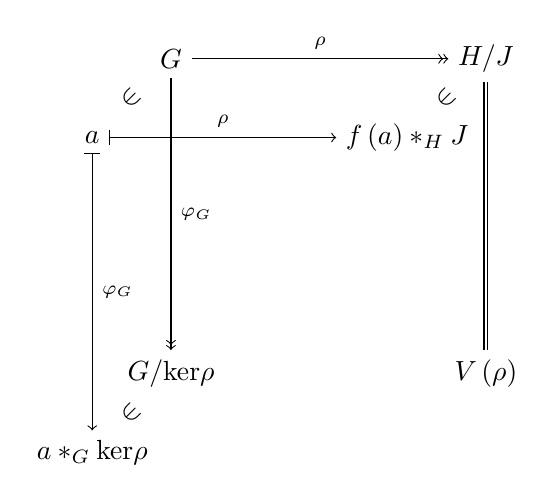
\begin{tikzpicture}[auto]
    \node[rotate=45] (x) at (4.5, 4.5) {$\in $};
    \node[rotate=45] (x) at (0.5, 0.5) {$\in $};
    \node[rotate=45] (x) at (0.5, 4.5) {$\in $};
    \node (c) at (4, 4) {$f\left( a\right) *_H J$};
    \node (e) at (5, 1) {$V\left( \rho \right) $};
    \node (g) at (5, 5) {$H/J$};
    \node (i) at (0, 0) {$a*_G {\rm ker} \rho $};
    \node (j) at (0, 4) {$a$};
    \node (k) at (1, 1) {$G/{\rm ker} \rho $};
    \node (l) at (1, 5) {$G$};
    \draw [->>] (l) to node {$\scriptstyle \rho $} (g);
    \draw [double distance=1pt] (g) to node {} (e);
    \draw [|->] (j) to node {$\scriptstyle \rho $} (c);
    \draw [|->] (j) to node {$\scriptstyle \varphi_G $} (i);
    \draw [->>] (l) to node {$\scriptstyle \varphi_G $} (k);
  \end{tikzpicture} 
\end{center}
$\ker\rho = I$が成り立つことに注意すれば、群準同型定理より次のようになるので、
\begin{center}
  \begin{tikzpicture}[auto]
    \node[rotate=45] (x) at (4.5, 4.5) {$\in $};
    \node[rotate=45] (x) at (0.5, 0.5) {$\in $};
    \node[rotate=45] (x) at (0.5, 4.5) {$\in $};
    \node (c) at (4, 4) {$f\left( a\right) *_H J$};
    \node (e) at (5, 1) {$H/J$};
    \node (g) at (5, 5) {$H/J$};
    \node (i) at (0, 0) {$a*_G I$};
    \node (j) at (0, 4) {$a$};
    \node (k) at (1, 1) {$G/I$};
    \node (l) at (1, 5) {$G$};
    \draw [->>] (l) to node {$\scriptstyle \rho $} (g);
    \draw [double distance=1pt] (g) to node {} (e);
    \draw [|->] (j) to node {$\scriptstyle \rho $} (c);
    \draw [|->] (j) to node {$\scriptstyle \varphi_G $} (i);
    \draw [->>] (l) to node {$\scriptstyle \varphi_G $} (k);
    \draw [>->>] (k) to node {} (e);
  \end{tikzpicture} 
\end{center}
$\left( {G}/{I},*_{G} \right) \cong \left( {H}/{J},*_{H} \right)$が成り立つ。
\end{proof}
\begin{thm}[第2群同型定理]\label{3.1.2.14}
群$(G,*)$の部分群$(H,*)$、正規部分群$(N,*)$が与えられたとする。このとき、次のことが成り立つ。
\begin{itemize}
\item
  群$(H*N,*)$はその群$(G,*)$の部分群である。
\item
  群$(H \cap N,*)$はその部分群$(H,*)$の正規部分群である、即ち、$(H \cap N,*) \trianglelefteq (H,*)$が成り立つ。
\item
  $\left( {H}/{(H \cap N)},* \right) \cong \left( {(H*N)}/{N},* \right)$が成り立つ。
\end{itemize}\par
この定理を第2群同型定理という。
\end{thm}
\begin{proof}
群$(G,*)$の部分群$(H,*)$、正規部分群$(N,*)$が与えられたとする。その群$(H,*)$自身もその群$(H,*)$の正規部分群であることに注意すれば、次のことが成り立つことは定理\ref{3.1.1.27}と定理\ref{3.1.1.28}より明らかである。
\begin{itemize}
\item
  群$(H*N,*)$はその群$(G,*)$の部分群である。
\item
  群$(H \cap N,*)$はその部分群$(H,*)$の正規部分群である。
\end{itemize}\par
このとき、$\ker f = N$が成り立つような群準同型写像$f$によるその群$(G,*)$の群準同型像$\left( G',*' \right)$が存在する。例えば、その群準同型写像$f$が自然な全射群準同型写像の場合などが挙げられる。ここで、その値域$V\left( f|H \right)$を$H'$とおくと、次のようになる。
\begin{center}
  \begin{tikzpicture}[auto]
    \node (y) at (3, 4) {$\subseteq $};
    \node (y) at (7, 4) {$\subseteq $};
    \node (y) at (7, 0) {$\subseteq $};
    \node (a) at (5, 4) {$V\left( f^{-1} |H'\right) $};
    \node (c) at (2, 4) {$H$};
    \node (d) at (2, 0) {$V\left( f|H\right) $};
    \node (e) at (6, 0) {$H'$};
    \node (i) at (8, 4) {$G$};
    \node (j) at (8, 0) {$G'$};
    \draw [->>] (c) to node {} (d);
    \draw [->>] (i) to node {$\scriptstyle f$} (j);
    \draw [double distance=1pt] (d) to node {} (e);
  \end{tikzpicture} 
\end{center}
$\forall a \in G$に対し、$a \in V\left( f^{- 1}|H' \right)$が成り立つなら、$f(a) \in V\left( f|H \right)$が成り立つので、$\exists h \in H$に対し、$f(a) = f(h)$が成り立つ。ここで、定理\ref{3.1.2.8}より$a \equiv h\ \mathrm{mod}\left( \ker f,* \right)$が成り立つ、即ち、$a \equiv h\ \mathrm{mod}(N,*)$が成り立つので、$h^{- 1}*a \in N$が成り立つ、即ち、次のようになる。
\begin{align*}
h*\left( h^{- 1}*a \right) &= \left( h*h^{- 1} \right)*a\\
&= 1_{(G,*)}*a\\
&= a \in h*N \subseteq H*N
\end{align*}
したがって、$V\left( f^{- 1}|H' \right) \subseteq H*N$が成り立つ。逆に、$\forall a \in G$に対し、$a \in H*N$が成り立つなら、$\exists h \in H\exists n \in N$に対し、$a = h*n$と書かれることができ、このとき、$n \in N = \ker f$が成り立つことに注意すれば、次のようになる。
\begin{align*}
f(a) &= f(h*n)\\
&= f(h)*'f(n)\\
&= f(h)*'1_{\left( G',*' \right)}\\
&= f(h)
\end{align*}
したがって、$f(a) \in V\left( f|H \right)$が得られるので、$a \in V\left( f^{- 1}|H' \right)$が成り立つ。したがって、$V\left( f^{- 1}|H' \right) \supseteq H*N$が成り立つ。以上より、$V\left( f^{- 1}|H' \right) = H*N$が得られ次式のようになる。
\begin{center}
  \begin{tikzpicture}[auto]
    \node (y) at (7, 4) {$\subseteq $};
    \node (y) at (7, 0) {$\subseteq $};
    \node (a) at (5, 4) {$V\left( f^{-1} |H'\right) $};
    \node (c) at (2, 4) {$H*N$};
    \node (e) at (6, 0) {$H'$};
    \node (i) at (8, 4) {$G$};
    \node (j) at (8, 0) {$G'$};
    \draw [->>] (i) to node {$\scriptstyle f$} (j);
    \draw [double distance=1pt] (c) to node {} (a);
  \end{tikzpicture} 
\end{center}
ここで、当然ながら$N \subseteq H*N$が成り立つので、第1群同型定理より次式のようになるので、
\begin{center}
  \begin{tikzpicture}[auto]
    \node (y) at (1, 4) {$\subseteq $};
    \node (y) at (7, 4) {$\subseteq $};
    \node (y) at (7, 0) {$\subseteq $};
    \node (a) at (5, 4) {$V\left( f^{-1} |H'\right) $};
    \node (c) at (2, 4) {$H*N$};
    \node (e) at (6, 0) {$H'$};
    \node (f) at (12, 4) {$\left( H*N\right) /N$};
    \node (i) at (8, 4) {$G$};
    \node (j) at (8, 0) {$G'$};
    \node (k) at (0, 4) {$N$};
    \draw [>->>] (f) to node {} (e);
    \draw [->>] (i) to node {$\scriptstyle f$} (j);
    \draw [double distance=1pt] (c) to node {} (a);
    \draw [->>] (c)[bend left=10] to node {} (f);
  \end{tikzpicture} 
\end{center}
$\left( {(H*N)}/{\ker f},* \right) = \left( {(H*N)}/{N},* \right) \cong \left( H',*' \right)$が成り立つ。\par
また、写像$f':H \rightarrow V\left( f|H \right);h \mapsto f(h)$は全射群準同型写像で、$\forall h \in G$に対し、$h \in \ker f'$が成り立つならそのときに限り、$h \in H$が成り立つかつ、$h \in \ker f$が成り立ち、したがって、これが成り立つならそのときに限り、$h \in H \cap N$が成り立つので、$\ker f' = H \cap N$が成り立つ。ここで、$(H,*) \trianglelefteq (H,*)$に注意すれば、定理\ref{3.1.1.28}より$(H \cap N,*) \trianglelefteq (H,*)$で第1群同型定理より次式のようになるので、
\begin{center}
  \begin{tikzpicture}[auto]
    \node (y) at (1, 4) {$\subseteq $};
    \node (c) at (2, 4) {$H$};
    \node (e) at (6, 0) {$H'$};
    \node (f) at (12, 4) {$H/\left( H\cap N\right) $};
    \node (i) at (8, 4) {$H$};
    \node (j) at (8, 0) {$V\left( f|H\right) $};
    \node (k) at (0, 4) {$H\cap N$};
    \draw [>->>] (f) to node {} (e);
    \draw [->>] (i) to node {$\scriptstyle f'$} (j);
    \draw [double distance=1pt] (c) to node {} (i);
    \draw [double distance=1pt] (e) to node {} (j);
    \draw [->>] (c)[bend left=10] to node {} (f);
  \end{tikzpicture} 
\end{center}
$\left( {H}/{(H \cap N)},* \right) \cong \left( H',*' \right)$が成り立つ。\par
以上より、$\left( {H}/{(H \cap N)},* \right) \cong \left( H',*' \right) \cong \left( {(H*N)}/{N},* \right)$が得られたので、$\left( {H}/{(H \cap N)},* \right) \cong \left( {(H*N)}/{N},* \right)$が成り立つ。
\end{proof}
\begin{thm}\label{3.1.2.15}
群々$\left( G,*_{G} \right)$、$\left( H,*_{H} \right)$の間の群準同型写像$f:G \rightarrow H$、その群$\left( G,*_{G} \right)$の正規部分群$\left( N,*_{G} \right)$が与えられたとき、$N \subseteq \ker f$が成り立つならそのときに限り、次式のような群準同型写像$\overline{f}$が存在する。
\begin{align*}
\overline{f}:{G}/{N} \rightarrow H;a*_{G}N \mapsto f(a)
\end{align*}
\end{thm}
\begin{proof}
群々$\left( G,*_{G} \right)$、$\left( H,*_{H} \right)$の間の群準同型写像$f:G \rightarrow H$、その群$\left( G,*_{G} \right)$の正規部分群$\left( N,*_{G} \right)$が与えられたとき、$N \subseteq \ker f$が成り立つなら、$\forall a,b \in N$に対し、$a*_{G}b^{- 1} \in N \subseteq \ker f$が成り立つので、次のようになる。
\begin{align*}
f(a) &= f(a)*_{H}1_{\left( H,*_{H} \right)}\\
&= f(a)*_{H}{f(b)}^{- 1}*_{H}f(b)\\
&= f(a)*_{H}f\left( b^{- 1} \right)*_{H}f(b)\\
&= f\left( a*_{G}b^{- 1} \right)*_{H}f(b)\\
&= 1_{\left( H,*_{H} \right)}*_{H}f(b)\\
&= f(b)
\end{align*}
したがって、$\forall f(a),f(b) \in H$に対し、$f(a) \neq f(b)$が成り立つなら、$a*_{G}b^{- 1} \notin N$が成り立つので、定理\ref{3.1.1.18}より$a*_{G}N \neq b*_{G}N$が成り立つ。対偶律により$\forall a*_{G}N,b*_{G}N \in {G}/{N}$に対し、$a*_{G}N = b*_{G}N$が成り立つなら、$f(a) = f(b)$が成り立つので、次式のような写像$\overline{f}$が存在する。
\begin{align*}
\overline{f}:{G}/{N} \rightarrow H;a*_{G}N \mapsto f(a)
\end{align*}
ここで、$\forall a*_{G}N,b*_{G}N \in {G}/{N}$に対し、定理\ref{3.1.1.29}より次のようになるので、
\begin{align*}
\overline{f}\left( a*_{G}N*_{G}b*_{G}N \right) &= \overline{f}\left( a*_{G}b*_{G}N \right)\\
&= f\left( a*_{G}b \right)\\
&= f(a)*_{H}f(b)\\
&= \overline{f}\left( a*_{G}N \right)*_{H}\overline{f}\left( b*_{G}N \right)
\end{align*}
その写像$\overline{f}$は群準同型写像である。\par
逆に、次式のような群準同型写像$\overline{f}$が存在するなら、
\begin{align*}
\overline{f}:{G}/{N} \rightarrow H;a*_{G}N \mapsto f(a)
\end{align*}
自然な全射群準同型写像$\varphi_{G}:G \twoheadrightarrow {G}/{N};a \mapsto a*_{G}N$を用いれば、定義より明らかに$f = \overline{f} \circ \varphi_{G}$が成り立つので、$\forall n \in N$に対し、定理\ref{3.1.2.1}より次のようになる。
\begin{align*}
f(h) &= \overline{f} \circ \varphi_{G}(n)\\
&= \overline{f}\left( n*_{G}N \right)\\
&= \overline{f}(N)\\
&= \overline{f}\left( 1_{\left( G,*_{G} \right)}*_{G}N \right)\\
&= f\left( 1_{\left( G,*_{G} \right)} \right)\\
&= 1_{\left( H,*_{H} \right)}
\end{align*}
これにより、$n \in \ker f$が成り立つので、$N \subseteq \ker f$が成り立つ。
\end{proof}
\begin{thm}[第3群同型定理]\label{3.1.2.16}
群$(G,*)$の正規部分群たち$(M,*)$、$(N,*)$が与えられ、$M \subseteq N$が成り立つとき、$\left( {G}/{N},* \right) \cong \left( {\left( {G}/{M} \right)}/{(N/M)},* \right)$が成り立つ。\par
この定理を第3群同型定理という。
\end{thm}
\begin{proof}
群$(G,*)$の正規部分群たち$(M,*)$、$(N,*)$が与えられ、$M \subseteq N$が成り立つとき、自然な全射群準同型写像$\varphi:G \twoheadrightarrow {G}/{N};a \mapsto a*N$を用いれば、定理\ref{3.1.2.7}より$M \subseteq N = \ker\varphi$が成り立つので、定理\ref{3.1.2.15}より次式のような群準同型写像$\overline{f}$が存在して
\begin{align*}
\overline{\varphi}:{G}/{M} \rightarrow {G}/{N};a*M \mapsto \varphi(a) = a*N
\end{align*}
次式のようになる。
\begin{center}
  \begin{tikzpicture}[auto]
    \node (a) at (0, 4) {$G/M$};
    \node (b) at (4, 4) {$G/N$};
    \node (c) at (0, 0) {$\left( G/M\right) /{\rm ker} \bar{\varphi } $};
    \node (d) at (4, 0) {$V\left( \bar{\varphi } |G/M\right) $};
    \node (e) at (4, 2) {\rotatebox{90}{$\subseteq $} };
    \node (f) at (2, 2) {$G$};
    \draw [->>] (f) to node {$\scriptstyle \varphi $} (b);
    \draw [->] (a) to node {$\scriptstyle \bar{\varphi } $} (b);
    \draw [->>] (a) to node {} (c);
  \end{tikzpicture} 
\end{center}
ここで、$\forall a*M \in \ker\overline{\varphi}$に対し、$\overline{\varphi}(a*M) = a*N = N$が成り立つならそのときに限り、$a \in N$が成り立つので、$a*M \in {N}/{M}$が成り立つ。したがって、$\ker\overline{\varphi} = {N}/{M}$が得られる。そこで、群準同型定理より次式のような写像$g:{\left( {G}/{M} \right)}/{\left( {N}/{M} \right)}\overset{\sim}{\rightarrow}V\left( \overline{\varphi}|{G}/{N} \right)$が存在する。
\begin{center}
  \begin{tikzpicture}[auto]
    \node (a) at (0, 4) {$G/M$};
    \node (b) at (4, 4) {$G/N$};
    \node (c) at (0, 0) {$\left( G/M\right) /\left( N/M\right) $};
    \node (d) at (4, 0) {$V\left( \bar{\varphi } |G/M\right) $};
    \node (e) at (4, 2) {\rotatebox{90}{$\subseteq $} };
    \node (f) at (2, 2) {$G$};
    \draw [->>] (f) to node {$\scriptstyle \varphi $} (b);
    \draw [->] (a) to node {$\scriptstyle \bar{\varphi } $} (b);
    \draw [->>] (a) to node {} (c);
    \draw [>->>] (c) to node {$\scriptstyle g$} (d);
  \end{tikzpicture} 
\end{center}
一方で、次式のような自然な全射群準同型写像$\varphi':G \twoheadrightarrow {G}/{M};a \mapsto a*M$が考えられれば、次のようになり
\begin{center}
  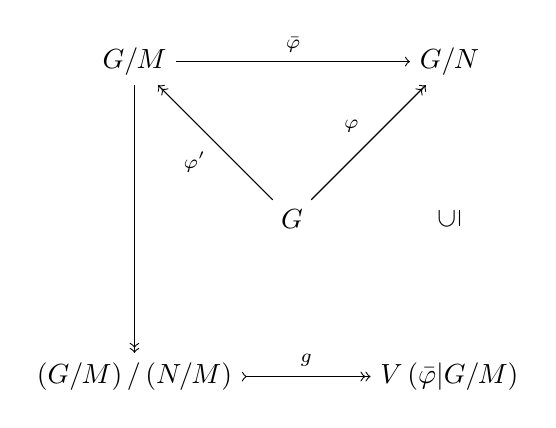
\begin{tikzpicture}[auto]
    \node (a) at (0, 4) {$G/M$};
    \node (b) at (4, 4) {$G/N$};
    \node (c) at (0, 0) {$\left( G/M\right) /\left( N/M\right) $};
    \node (d) at (4, 0) {$V\left( \bar{\varphi } |G/M\right) $};
    \node (e) at (4, 2) {\rotatebox{90}{$\subseteq $} };
    \node (f) at (2, 2) {$G$};
    \draw [->>] (f) to node {$\scriptstyle \varphi' $} (a);
    \draw [->>] (f) to node {$\scriptstyle \varphi $} (b);
    \draw [->] (a) to node {$\scriptstyle \bar{\varphi } $} (b);
    \draw [->>] (a) to node {} (c);
    \draw [>->>] (c) to node {$\scriptstyle g$} (d);
  \end{tikzpicture} 
\end{center}
$\varphi = \overline{\varphi} \circ \varphi'$が成り立つので、$\forall\overline{\varphi}(a*M) \in V\left( \overline{\varphi}|{G}/{M} \right)$に対し、次のようになるので、
\begin{align*}
\overline{\varphi}(a*M) &= \overline{\varphi}\left( \varphi'(a) \right)\\
&= \overline{\varphi} \circ \varphi'(a)\\
&= \varphi(a) \in V(\varphi)
\end{align*}
その写像$\varphi$が全射であることに注意すれば、$\overline{\varphi}(a*M) \in V\left( \overline{\varphi}|{G}/{M} \right)$が成り立つならそのときに限り、$\varphi(a) \in {G}/{N}$が成り立つので、次式のようになる。
\begin{center}
  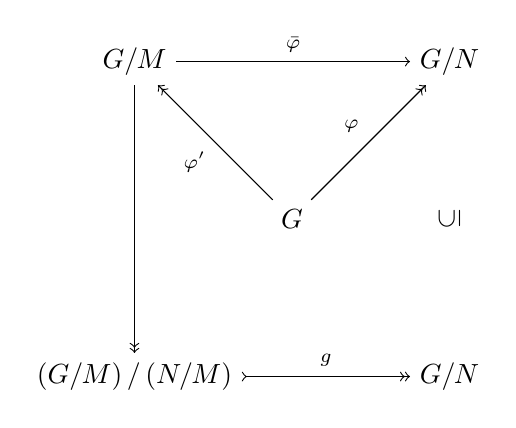
\begin{tikzpicture}[auto]
    \node (a) at (0, 4) {$G/M$};
    \node (b) at (4, 4) {$G/N$};
    \node (c) at (0, 0) {$\left( G/M\right) /\left( N/M\right) $};
    \node (d) at (4, 0) {$G/N$};
    \node (e) at (4, 2) {\rotatebox{90}{$\subseteq $} };
    \node (f) at (2, 2) {$G$};
    \draw [->>] (f) to node {$\scriptstyle \varphi' $} (a);
    \draw [->>] (f) to node {$\scriptstyle \varphi $} (b);
    \draw [->] (a) to node {$\scriptstyle \bar{\varphi } $} (b);
    \draw [->>] (a) to node {} (c);
    \draw [>->>] (c) to node {$\scriptstyle g$} (d);
  \end{tikzpicture} 
\end{center}
したがって、$\left( {G}/{N},* \right) \cong \left( {\left( {G}/{M} \right)}/{(N/M)},* \right)$が成り立つ。
\end{proof}
\begin{thebibliography}{50}
  \bibitem{1}
  松坂和夫, 代数系入門, 岩波書店, 1976. 新装版第2刷 p65-71 ISBN978-4-00-029873-5
  \bibitem{2}
  よしいず. "群の同型定理". MATHEMATICS.PDF. \url{https://mathematics-pdf.com/pdf/grp_iso_thm.pdf} (2021-8-8 15:30 取得)
  \bibitem{3}
  花木章秀. "群論". 信州大学. \url{http://math.shinshu-u.ac.jp/~hanaki/edu/group/group2011pre.pdf} (2021-8-8 16:00 取得)
\end{thebibliography}
\end{document}

\clearpage
\documentclass[dvipdfmx]{jsarticle}
\setcounter{section}{1}
\setcounter{subsection}{2}
\usepackage{xr}
\externaldocument{3.1.1}
\externaldocument{3.1.2}
\usepackage{amsmath,amsfonts,amssymb,array,comment,mathtools,url,docmute}
\usepackage{longtable,booktabs,dcolumn,tabularx,mathtools,multirow,colortbl,xcolor}
\usepackage[dvipdfmx]{graphics}
\usepackage{bmpsize}
\usepackage{amsthm}
\usepackage{enumitem}
\setlistdepth{20}
\renewlist{itemize}{itemize}{20}
\setlist[itemize]{label=•}
\renewlist{enumerate}{enumerate}{20}
\setlist[enumerate]{label=\arabic*.}
\setcounter{MaxMatrixCols}{20}
\setcounter{tocdepth}{3}
\newcommand{\rotin}{\text{\rotatebox[origin=c]{90}{$\in $}}}
\newcommand{\amap}[6]{\text{\raisebox{-0.7cm}{\begin{tikzpicture} 
  \node (a) at (0, 1) {$\textstyle{#2}$};
  \node (b) at (#6, 1) {$\textstyle{#3}$};
  \node (c) at (0, 0) {$\textstyle{#4}$};
  \node (d) at (#6, 0) {$\textstyle{#5}$};
  \node (x) at (0, 0.5) {$\rotin $};
  \node (x) at (#6, 0.5) {$\rotin $};
  \draw[->] (a) to node[xshift=0pt, yshift=7pt] {$\textstyle{\scriptstyle{#1}}$} (b);
  \draw[|->] (c) to node[xshift=0pt, yshift=7pt] {$\textstyle{\scriptstyle{#1}}$} (d);
\end{tikzpicture}}}}
\newcommand{\twomaps}[9]{\text{\raisebox{-0.7cm}{\begin{tikzpicture} 
  \node (a) at (0, 1) {$\textstyle{#3}$};
  \node (b) at (#9, 1) {$\textstyle{#4}$};
  \node (c) at (#9+#9, 1) {$\textstyle{#5}$};
  \node (d) at (0, 0) {$\textstyle{#6}$};
  \node (e) at (#9, 0) {$\textstyle{#7}$};
  \node (f) at (#9+#9, 0) {$\textstyle{#8}$};
  \node (x) at (0, 0.5) {$\rotin $};
  \node (x) at (#9, 0.5) {$\rotin $};
  \node (x) at (#9+#9, 0.5) {$\rotin $};
  \draw[->] (a) to node[xshift=0pt, yshift=7pt] {$\textstyle{\scriptstyle{#1}}$} (b);
  \draw[|->] (d) to node[xshift=0pt, yshift=7pt] {$\textstyle{\scriptstyle{#2}}$} (e);
  \draw[->] (b) to node[xshift=0pt, yshift=7pt] {$\textstyle{\scriptstyle{#1}}$} (c);
  \draw[|->] (e) to node[xshift=0pt, yshift=7pt] {$\textstyle{\scriptstyle{#2}}$} (f);
\end{tikzpicture}}}}
\renewcommand{\thesection}{第\arabic{section}部}
\renewcommand{\thesubsection}{\arabic{section}.\arabic{subsection}}
\renewcommand{\thesubsubsection}{\arabic{section}.\arabic{subsection}.\arabic{subsubsection}}
\everymath{\displaystyle}
\allowdisplaybreaks[4]
\usepackage{vtable}
\theoremstyle{definition}
\newtheorem{thm}{定理}[subsection]
\newtheorem*{thm*}{定理}
\newtheorem{dfn}{定義}[subsection]
\newtheorem*{dfn*}{定義}
\newtheorem{axs}[dfn]{公理}
\newtheorem*{axs*}{公理}
\renewcommand{\headfont}{\bfseries}
\makeatletter
  \renewcommand{\section}{%
    \@startsection{section}{1}{\z@}%
    {\Cvs}{\Cvs}%
    {\normalfont\huge\headfont\raggedright}}
\makeatother
\makeatletter
  \renewcommand{\subsection}{%
    \@startsection{subsection}{2}{\z@}%
    {0.5\Cvs}{0.5\Cvs}%
    {\normalfont\LARGE\headfont\raggedright}}
\makeatother
\makeatletter
  \renewcommand{\subsubsection}{%
    \@startsection{subsubsection}{3}{\z@}%
    {0.4\Cvs}{0.4\Cvs}%
    {\normalfont\Large\headfont\raggedright}}
\makeatother
\makeatletter
\renewenvironment{proof}[1][\proofname]{\par
  \pushQED{\qed}%
  \normalfont \topsep6\p@\@plus6\p@\relax
  \trivlist
  \item\relax
  {
  #1\@addpunct{.}}\hspace\labelsep\ignorespaces
}{%
  \popQED\endtrivlist\@endpefalse
}
\makeatother
\renewcommand{\proofname}{\textbf{証明}}
\usepackage{tikz,graphics}
\usepackage[dvipdfmx]{hyperref}
\usepackage{pxjahyper}
\hypersetup{
 setpagesize=false,
 bookmarks=true,
 bookmarksdepth=tocdepth,
 bookmarksnumbered=true,
 colorlinks=false,
 pdftitle={},
 pdfsubject={},
 pdfauthor={},
 pdfkeywords={}}
\begin{document}
%\hypertarget{ux5171ux5f79ux985e}{%
\subsection{共役類}%\label{ux5171ux5f79ux985e}}
%\hypertarget{ux81eaux5df1ux7fa4ux540cux578bux5199ux50cf}{%
\subsubsection{自己群同型写像}%\label{ux81eaux5df1ux7fa4ux540cux578bux5199ux50cf}}
\begin{dfn}
群$(G,*)$について、群同型写像$f:G\overset{\sim}{\rightarrow}G$をその群$(G,*)$の自己群同型写像という。このような写像全体の集合を$\mathrm{aut}(G,*)$とおく。
\end{dfn}\par
例えば、可換群$(G,*)$における写像$\bullet^{- 1}:G\overset{\sim}{\rightarrow}G;a \mapsto a^{- 1}$が挙げられる。
\begin{thm}\label{3.1.3.1}
群$(G,*)$について、その組$\left( \mathrm{aut}(G,*), \circ \right)$は群をなす。
\end{thm}
\begin{dfn}
群$(G,*)$について、その群$\left( \mathrm{aut}(G,*), \circ \right)$をその群$(G,*)$の自己群同型群という。
\end{dfn}
\begin{proof}
  群$(G,*)$が与えられたとき、その組$\left( \mathrm{aut}(G,*), \circ \right)$について、恒等写像$I_G :G\rightarrow G; a\mapsto a$を用いれば、$\forall f,g,h\in \mathrm{aut}(G,*)$に対し、写像の合成の結合律より$f\circ \left(g \circ h\right) =\left(f \circ g\right) \circ h$が成り立つ。さらに、$\forall f\in \mathrm{aut}(G,*)$に対し、$f\circ I_G =I_G \circ f =f$が成り立つ。最後に、$\forall f\in \mathrm{aut}(G,*)$に対し、その逆写像$f^{-1}$も存在して、$f^{-1}\in \mathrm{aut}(G,*)$なので、$f\circ f^{-1} =f^{-1} \circ f=I_G $が成り立つ。よって、示すべきことが示された。
\end{proof}
\begin{thm}\label{3.1.3.2}
群$(G,*)$について、$\forall s \in G$に対し、次式のように定義される写像$\sigma_{s}$は$\sigma_{s} \in \mathrm{aut}(G,*)$を満たす、即ち、自己群同型写像となる。
\begin{align*}
\sigma_{s}:G \rightarrow G;a \mapsto s^{- 1}*a*s
\end{align*}
\end{thm}
\begin{dfn}
群$(G,*)$について、上の自己群同型写像$\sigma_{s}$をその群$(G,*)$における内部自己群同型写像という。
\end{dfn}
\begin{proof}
群$(G,*)$について、$\forall s \in G$に対し、次式のように定義される写像$\sigma_{s}$において、
\begin{align*}
\sigma_{s}:G \rightarrow G;a \mapsto s^{- 1}*a*s
\end{align*}
$\forall a,b \in G$に対し、次のようになることから、
\begin{align*}
\sigma_{s}(a*b) &= s^{- 1}*a*b*s\\
&= s^{- 1}*a*1_{(G,*)}*b*s\\
&= s^{- 1}*a*s*s^{- 1}*b*s\\
&= \sigma_{s}(a)*\sigma_{s}(b)
\end{align*}
その写像$\sigma_{s}$は群準同型写像である。さらに、$\forall a \in G$に対し、次のようになることから、
\begin{align*}
\sigma_{s^{- 1}} \circ \sigma_{s}(a) &= \sigma_{s^{- 1}}\left( \sigma_{s}(a) \right)\\
&= \sigma_{s^{- 1}}\left( s^{- 1}*a*s \right)\\
&= \left( s^{- 1} \right)^{- 1}*s^{- 1}*a*s*s^{- 1}\\
&= 1_{(G,*)}*a*1_{(G,*)} = a\\
\sigma_{s} \circ \sigma_{s^{- 1}}(a) &= \sigma_{s}\left( \sigma_{s^{- 1}}(a) \right)\\
&= \sigma_{s}\left( \left( s^{- 1} \right)^{- 1}*a*s^{- 1} \right)\\
&= s^{- 1}*\left( s^{- 1} \right)^{- 1}*a*s^{- 1}*s\\
&= 1_{(G,*)}*a*1_{(G,*)} = a
\end{align*}
$\sigma_{s}^{- 1} = \sigma_{s^{- 1}}$が成り立つので、その写像$\sigma_{s}$はたしかに自己群同型写像となる。
\end{proof}
\begin{thm}\label{3.1.3.3}
群$(G,*)$について、$\forall z \in G$に対し、$\sigma_{z} = I_{G}$が成り立つならそのときに限り、その群$(G,*)$の中心を$Z(G)$として、$z \in Z(G)$が成り立つ。
\end{thm}
\begin{proof}
群$(G,*)$について、$\forall z \in G$に対し、$\sigma_{z} = I_{G}$が成り立つなら、$\forall a \in G$に対し、$z^{- 1}*a*z = a$が成り立ち、したがって、$z*a = a*z$が成り立つ。これにより、その群$(G,*)$の中心を$Z(G)$として、$z \in Z(G)$が成り立つ。\par
逆に、$z \in Z(G)$が成り立つなら、$\forall a\in G$に対し、$z*a=a*z$が成り立つので、次のようになる。
\begin{align*}
  \sigma_z (a) &=z^{-1} *a*z \\
  &=z^{-1} *z*a\\
  &=1_{(G,*)} *a=a
\end{align*}
よって、$\sigma_{z} = I_{G}$が成り立つ。
\end{proof}
\begin{thm}\label{3.1.3.4}
群$(G,*)$について、次のことは同値である。
\begin{itemize}
\item
  その群$(G,*)$は可換群である。
\item
  $\bullet^{- 1}:G\overset{\sim}{\rightarrow}G;a \mapsto a^{- 1} \in \mathrm{aut}(G,*)$が成り立つ。
\end{itemize}
\end{thm}
\begin{proof}
群$(G,*)$について、その群$(G,*)$は可換群であるなら、写像$\bullet^{- 1}:G\overset{\sim}{\rightarrow}G;a \mapsto a^{- 1}$について、これはもちろん、全単射である。さらに、$\forall a,b \in G$に対し、次のようになることから、
\begin{align*}
\bullet^{- 1}(a*b) &= (a*b)^{- 1}\\
&= b^{- 1}*a^{- 1}\\
&= a^{- 1}*b^{- 1}\\
&= \bullet^{- 1}(a)* \bullet^{- 1}(b)
\end{align*}
その写像$\bullet^{- 1}$は群同型写像となる。\par
逆に、$\bullet^{- 1}:G\overset{\sim}{\rightarrow}G;a \mapsto a^{- 1} \in \mathrm{aut}(G,*)$が成り立つなら、定理\ref{3.1.2.3}より次のようになることから、
\begin{align*}
a*b &= \left( \bullet^{- 1} \right)^{- 1} \circ \bullet^{- 1}(a*b)\\
&= \left( \bullet^{- 1} \right)^{- 1} \circ \left( \bullet^{- 1}(a)* \bullet^{- 1}(b) \right)\\
&= \left( \bullet^{- 1} \right)^{- 1} \circ \left( a^{- 1}*b^{- 1} \right)\\
&= \left( \bullet^{- 1} \right)^{- 1} \circ (b*a)^{- 1}\\
&= \left( \bullet^{- 1} \right)^{- 1} \circ \bullet^{- 1}(b*a)\\
&= b*a
\end{align*}
その群$(G,*)$は可換群である。
\end{proof}
%\hypertarget{ux5171ux5f79ux985e-1}{%
\subsubsection{共役類}%\label{ux5171ux5f79ux985e-1}}
\begin{thm}\label{3.1.3.5}
群$(G,*)$について、その集合$G$の2元$a$、$b$が与えられたとき、$\exists s \in G$に対し、$\sigma_{s}(a) = b$が成り立つことを$aR_{\sigma}b$とおくことにすると、その関係$R_{\sigma}$は同値関係となる。
\end{thm}
\begin{dfn}
群$(G,*)$について、その集合$G$の2元$a$、$b$が与えられたとき、$aR_{\sigma}b$が成り立つことをそれらの元々$a$、$b$は互いに共役であるという。さらに、その同値類$C_{R_{\sigma}}(a)$をその群$(G,*)$の共役類という。
\end{dfn}
\begin{proof}
群$(G,*)$について、その集合$G$の2元$a$、$b$が与えられたとき、$\exists s \in G$に対し、$\sigma_{s}(a) = b$が成り立つことを$aR_{\sigma}b$とおくことにする。このとき、$\forall a \in G$に対し、次式が成り立つことから、
\begin{align*}
a &= 1_{(G,*)}*a*1_{(G,*)}\\
&= 1_{(G,*)}^{- 1}*a*1_{(G,*)}\\
&= \sigma_{1_{(G,*)}}(a)
\end{align*}
$aR_{\sigma}a$が成り立つ。\par
$\forall a,b \in G$に対し、$aR_{\sigma}b$が成り立つなら、$\exists s \in G$に対し、$\sigma_{s}(a) = b$が成り立つ、即ち、$s^{- 1}*a*s = b$が成り立つので、$\exists s^{- 1} \in G$に対し、次のようになることから、
\begin{align*}
\sigma_{s^{- 1}}(b) &= \left( s^{- 1} \right)^{- 1}*b*s^{- 1}\\
&= \left( s^{- 1} \right)^{- 1}*s^{- 1}*a*s*s^{- 1}\\
&= 1_{(G,*)}*a*1_{(G,*)}\\
&= a
\end{align*}
$bR_{\sigma}a$が成り立つ。\par
$\forall a,b,c \in G$に対し、$aR_{\sigma}b$かつ$bR_{\sigma}c$が成り立つなら、$\exists s,t \in G$に対し、$\sigma_{s}(a) = b$かつ$\sigma_{t}(b) = c$が成り立つので、次のようになることから、
\begin{align*}
c &= \sigma_{t}(b)\\
&= \sigma_{t}\left( \sigma_{s}(a) \right)\\
&= \sigma_{t}\left( s^{- 1}*a*s \right)\\
&= t^{- 1}*s^{- 1}a*s*t\\
&= (s*t)^{- 1}*a*(s*t)\\
&= \sigma_{s*t}(a)
\end{align*}
$\exists s*t \in G$に対し、$\sigma_{s*t}(a) = c$が成り立つ。これにより、$aR_{\sigma}c$が成り立つ。\par
よって、その関係$R_{\sigma}$は同値関係となる。
\end{proof}
\begin{thm}\label{3.1.3.6}
有限な群$(G,*)$について、その集合$G$の1つの元$a$が与えられたとき、その元$a$の共役類の元の個数は自然数$\left( G:N\left( G,\left\{ a \right\} \right) \right)$に等しい、即ち、$\#{C_{R_{\sigma}}(a)} = \left( G:N\left( G,\left\{ a \right\} \right) \right)$が成り立つ。
\end{thm}
\begin{proof}
有限な群$(G,*)$について、その集合$G$の1つの元$a$が与えられたとき、次のようになることから、
\begin{align*}
C_{R_{\sigma}}(a) &= \left\{ b \in G \middle| aR_{\sigma}b \right\}\\
&= \left\{ b \in G \middle| \exists s \in G\left\lbrack \sigma_{s}(a) = s^{- 1}*a*s = b \right\rbrack \right\}\\
&= \left\{ s^{- 1}*a*s \in G \middle| s \in G \right\}
\end{align*}
正規化群$\left( N\left( G,\left\{ a \right\} \right),* \right)$について、次のような写像たち$f$、$g$が考えられよう。
\begin{align*}
f:C_{R_{\sigma}}(a) \rightarrow {G}/_l {N\left( G,\left\{ a \right\} \right)};s^{- 1}*a*s \mapsto s^{- 1}*N\left( G,\left\{ a \right\} \right),\\
g:{G}/_l {N\left( G,\left\{ a \right\} \right)} \rightarrow C_{R_{\sigma}}(a);s*N\left( G,\left\{ a \right\} \right) \mapsto s*a*s^{- 1}
\end{align*}\par
$\forall s^{- 1}*a*s,t^{- 1}*a*t \in C_{R_{\sigma}}(a)$に対し、$s^{- 1}*a*s = t^{- 1}*a*t$が成り立つとする。このとき、$a*s*t^{- 1} = s*t^{- 1}*a$が成り立つので、$s*t^{- 1} \in N\left( G,\left\{ a \right\} \right)$が成り立つ。したがって、次のようになり、
\begin{align*}
s*t^{- 1} \in N\left( G,\left\{ a \right\} \right) &\Leftrightarrow \left( s^{- 1} \right)^{- 1}*t^{- 1} \in N\left( G,\left\{ a \right\} \right)\\
&\Leftrightarrow t^{- 1} \in s^{- 1}*N\left( G,\left\{ a \right\} \right)\\
&\Leftrightarrow t^{- 1} \in C_{\equiv_{l}\ \mathrm{mod}\left( N\left( G,\left\{ a \right\} \right),* \right)}\left( s^{- 1} \right)\\
&\Leftrightarrow t^{- 1} \in C_{\equiv_{l}\ \mathrm{mod}\left( N\left( G,\left\{ a \right\} \right),* \right)}\left( s^{- 1} \right) \land t^{- 1} \equiv_{l}t^{- 1}\ \mathrm{mod}\left( N\left( G,\left\{ a \right\} \right),* \right)\\
&\Leftrightarrow t^{- 1} \in C_{\equiv_{l}\ \mathrm{mod}\left( N\left( G,\left\{ a \right\} \right),* \right)}\left( s^{- 1} \right) \land t^{- 1} \in C_{\equiv_{l}\ \mathrm{mod}\left( N\left( G,\left\{ a \right\} \right),* \right)}\left( t^{- 1} \right)\\
&\Leftrightarrow t^{- 1} \in C_{\equiv_{l}\ \mathrm{mod}\left( N\left( G,\left\{ a \right\} \right),* \right)}\left( s^{- 1} \right) \cap C_{\equiv_{l}\ \mathrm{mod}\left( N\left( G,\left\{ a \right\} \right),* \right)}\left( t^{- 1} \right)
\end{align*}
同値類の性質より$C_{\equiv_{l}\ \mathrm{mod}\left( N\left( G,\left\{ a \right\} \right),* \right)}\left( s^{- 1} \right) = C_{\equiv_{l}\ \mathrm{mod}\left( N\left( G,\left\{ a \right\} \right),* \right)}\left( t^{- 1} \right)$が成り立つので、定理\ref{3.1.1.13}より次のようになる。
\begin{align*}
f\left( s^{- 1}*a*s \right) &= s^{- 1}*N\left( G,\left\{ a \right\} \right)\\
&= C_{\equiv_{l}\ \mathrm{mod}\left( N\left( G,\left\{ a \right\} \right),* \right)}\left( s^{- 1} \right)\\
&= C_{\equiv_{l}\ \mathrm{mod}\left( N\left( G,\left\{ a \right\} \right),* \right)}\left( t^{- 1} \right)\\
&= t^{- 1}*N\left( G,\left\{ a \right\} \right)\\
&= f\left( t^{- 1}*a*t \right)
\end{align*}
これにより、その対応$f$は確かに写像となっている。\par
また、$\forall s*N\left( G,\left\{ a \right\} \right),t*N\left( G,\left\{ a \right\} \right) \in Q_{l}$に対し、$s*N\left( G,\left\{ a \right\} \right) = t*N\left( G,\left\{ a \right\} \right)$が成り立つとする。このとき、定理\ref{3.1.1.13}より$C_{\equiv_{l}\ \mathrm{mod}\left( N\left( G,\left\{ a \right\} \right),* \right)}(s) = C_{\equiv_{l}\ \mathrm{mod}\left( N\left( G,\left\{ a \right\} \right),* \right)}(t)$が成り立つので、$s \in C_{\equiv_{l}\ \mathrm{mod}\left( N\left( G,\left\{ a \right\} \right),* \right)}(t)$が成り立ち、したがって、$s \equiv_{l}t\ \mathrm{mod}\left( N\left( G,\left\{ a \right\} \right),* \right)$が成り立つ。これにより、$s^{- 1}*t \in N\left( G,\left\{ a \right\} \right)$が成り立つので、$s^{- 1}*t*a = a*s^{- 1}*t$が得られ、したがって、$s*a*s^{- 1} = t*a*t^{- 1}$が成り立つ。よって、次式が成り立つので、
\begin{align*}
g\left( s*N\left( G,\left\{ a \right\} \right) \right) &= s*a*s^{- 1}\\
&= t*a*t^{- 1}\\
&= g\left( t*N\left( G,\left\{ a \right\} \right) \right)
\end{align*}
その対応$g$は確かに写像となっている。\par
このとき、$\forall s^{- 1}*a*s \in C_{R_{\sigma}}(a)$に対し、次のようになるかつ、
\begin{align*}
g \circ f\left( s^{- 1}*a*s \right) &= g\left( s^{- 1}*N\left( G,\left\{ a \right\} \right) \right)\\
&= s^{- 1}*a*\left( s^{- 1} \right)^{- 1}\\
&= s^{- 1}*a*s
\end{align*}
$\forall s*N\left( G,\left\{ a \right\} \right) \in {G}/_l {N\left( G,\left\{ a \right\} \right)}$に対し、次のようになることから、
\begin{align*}
f \circ g\left( s*N\left( G,\left\{ a \right\} \right) \right) = f\left( s*a*s^{- 1} \right) = f\left( \left( s^{- 1} \right)^{- 1}*a*s^{- 1} \right) = s^{- 1}*N\left( G,\left\{ a \right\} \right)
\end{align*}
$g = f^{- 1}$が成り立つ。これにより、それらの集合たち$C_{R_{\sigma}}(a)$、${G}/_l {N\left( G,\left\{ a \right\} \right)} $との間に全単射な写像が存在するので、次のようになる。
\begin{align*}
\#{C_{R_{\sigma}}(a)} &= \#{G}/_l {N\left( G,\left\{ a \right\} \right)}\\
&= \left( G:N\left( G,\left\{ a \right\} \right) \right)
\end{align*}
\end{proof}
%\hypertarget{ux985eux7b49ux5f0f}{%
\subsubsection{類等式}%\label{ux985eux7b49ux5f0f}}
\begin{thm}\label{3.1.3.7}
有限な群$(G,*)$について、その集合$G$の1つの元$a$が与えられたとき、次のことは同値である。
\begin{itemize}
\item
  $C_{R_{\sigma}}(a) = \left\{ a \right\}$が成り立つ。
\item
  $\left( G:N\left( G,\left\{ a \right\} \right) \right) = 1$が成り立つ。
\item
  その群$(G,*)$の中心を$Z(G)$として$a \in Z(G)$が成り立つ。
\end{itemize}
\end{thm}
\begin{proof}
有限な群$(G,*)$について、その集合$G$の1つの元$a$が与えられたとき、$C_{R_{\sigma}}(a) = \left\{ a \right\}$が成り立つなら、定理\ref{3.1.3.6}より$\left( G:N\left( G,\left\{ a \right\} \right) \right) = 1$が成り立つ。\par
逆に、$\left( G:N\left( G,\left\{ a \right\} \right) \right) = 1$が成り立つなら、もちろん、集合$1_{(G,*)}*N\left( G,\left\{ a \right\} \right)$は正規化群$\left( N\left( G,\left\{ a \right\} \right),* \right)$を法とする左剰余類であるので、$N\left( G,\left\{ a \right\} \right) \subseteq G$が成り立つかつ、$\forall b \in G$に対し、$b*N\left( G,\left\{ a \right\} \right) = 1_{(G,*)}*N\left( G,\left\{ a \right\} \right) = N\left( G,\left\{ a \right\} \right)$が成り立つことから、$b = b*1_{(G,*)} \in b*N\left( G,\left\{ a \right\} \right) = N\left( G,\left\{ a \right\} \right)$が成り立ち、したがって、$G = N\left( G,\left\{ a \right\} \right)$が成り立つ。もちろん、$a \in C_{R_{\sigma}}(a)$が成り立つかつ、$\forall b \in C_{R_{\sigma}}(a)$に対し、$aR_{\sigma}b$が成り立つなら、$\exists s \in G$に対し、$s^{- 1}*a*s = b$が成り立ち、$s \in N\left( G,\left\{ a \right\} \right)$が成り立つので、$a*s = s*a$が成り立つことから、次のようになるので、
\begin{align*}
b &= s^{- 1}*a*s\\
&= s^{- 1}*s*a\\
&= 1_{(G,*)}*a = a
\end{align*}
$b \in \left\{ a \right\}$が成り立つ。これにより、$C_{R_{\sigma}}(a) = \left\{ a \right\}$が成り立つ。\par
また、$\left( G:N\left( G,\left\{ a \right\} \right) \right) = 1$が成り立つなら、上記の議論と同様にして、$G = N\left( G,\left\{ a \right\} \right)$が成り立つことが示される。ここで、$\forall b \in G$に対し、$b \in N\left( G,\left\{ a \right\} \right)$が成り立つので、$b*a = a*b$が成り立つ。これにより、$a \in Z(G)$が成り立つ。\par
逆に、$a \in Z(G)$が成り立つとき、もちろん、$a \in C_{R_{\sigma}}(a)$が成り立つかつ、$\forall b \in C_{R_{\sigma}}(a)$に対し、$aR_{\sigma}b$が成り立つなら、$\exists s \in G$に対し、$s^{- 1}*a*s = b$が成り立ち、$a \in Z(G)$が成り立つので、$a*s = s*a$が成り立つことから、次のようになるので、
\begin{align*}
b = s^{- 1}*a*s = s^{- 1}*s*a = 1_{(G,*)}*a = a
\end{align*}
$b \in \left\{ a \right\}$が成り立つ。これにより、$C_{R_{\sigma}}(a) = \left\{ a \right\}$が成り立つ。\par
以上の議論により、次のことは同値である。
\begin{itemize}
\item
  $C_{R_{\sigma}}(a) = \left\{ a \right\}$が成り立つ。
\item
  $\left( G:N\left( G,\left\{ a \right\} \right) \right) = 1$が成り立つ。
\item
  その群$(G,*)$の中心を$Z(G)$として$a \in Z(G)$が成り立つ。
\end{itemize}
\end{proof}
\begin{thm}[類等式]\label{3.1.3.8}
有限な群$(G,*)$について、その群$(G,*)$の中心$Z(G)$を用いて考えられれば、次式が成り立つ。
\begin{align*}
o(G,*) = o\left( Z(G),* \right) + \sum_{\scriptsize \begin{matrix} C_{R_{\sigma}}(a) \in {G}/{R_{\sigma}} \\a \notin Z(G) \end{matrix}} \left( G:N\left( G,\left\{ a \right\} \right) \right)
\end{align*}\par
この式を類等式という。
\end{thm}
\begin{proof}
有限な群$(G,*)$について、その群$(G,*)$の中心$Z(G)$を用いて考えられれば、定理\ref{3.1.3.4}と同値類に関する一定理より次式が成り立つ。
\begin{align*}
G &= \bigsqcup_{} {G}/{R_{\sigma}}\\
&= \bigsqcup_{C_{R_{\sigma}}(a) \in {G}/{R_{\sigma}}} {C_{R_{\sigma}}(a)}\\
&= \bigsqcup_{\scriptsize \begin{matrix} C_{R_{\sigma}}(a) \in {G}/{R_{\sigma}} \\a \in Z(G) \end{matrix}} {C_{R_{\sigma}}(a)} + \bigsqcup_{\scriptsize \begin{matrix} C_{R_{\sigma}}(a) \in {G}/{R_{\sigma}} \\a \notin Z(G) \end{matrix}} {C_{R_{\sigma}}(a)}
\end{align*}
定理\ref{3.1.1.42}、定理\ref{3.1.3.6}、定理\ref{3.1.3.7}より$a,b \in Z(G)$のとき、$a \neq b$が成り立つなら、$C_{R_{\sigma}}(a) = \left\{ a \right\} \neq \left\{ b \right\} = C_{R_{\sigma}}(b)$が成り立つことに注意すれば、したがって、次のようになる。
\begin{align*}
o(G,*) &= \#G\\
&= \#\left( \bigsqcup_{\scriptsize \begin{matrix} C_{R_{\sigma}}(a) \in {G}/{R_{\sigma}} \\a \in Z(G) \end{matrix}} {C_{R_{\sigma}}(a)} + \bigsqcup_{\scriptsize \begin{matrix} C_{R_{\sigma}}(a) \in {G}/{R_{\sigma}} \\a \notin Z(G) \end{matrix}} {C_{R_{\sigma}}(a)} \right)\\
&= \sum_{\scriptsize \begin{matrix} C_{R_{\sigma}}(a) \in {G}/{R_{\sigma}} \\a \in Z(G) \end{matrix}} {\#{C_{R_{\sigma}}(a)}} + \sum_{\scriptsize \begin{matrix} C_{R_{\sigma}}(a) \in {G}/{R_{\sigma}} \\a \notin Z(G) \end{matrix}} {\#{C_{R_{\sigma}}(a)}}\\
&= \sum_{\scriptsize \begin{matrix} C_{R_{\sigma}}(a) \in {G}/{R_{\sigma}} \\a \in Z(G) \end{matrix}} \left( G:N\left( G,\left\{ a \right\} \right) \right) + \sum_{\scriptsize \begin{matrix} C_{R_{\sigma}}(a) \in {G}/{R_{\sigma}} \\a \notin Z(G) \end{matrix}} \left( G:N\left( G,\left\{ a \right\} \right) \right)\\
&= \sum_{\scriptsize \begin{matrix} C_{R_{\sigma}}(a) \in {G}/{R_{\sigma}} \\a \in Z(G) \end{matrix}} 1 + \sum_{\scriptsize \begin{matrix} C_{R_{\sigma}}(a) \in {G}/{R_{\sigma}} \\a \notin Z(G) \end{matrix}} \left( G:N\left( G,\left\{ a \right\} \right) \right)\\
&= \#{Z(G)} + \sum_{\scriptsize \begin{matrix} C_{R_{\sigma}}(a) \in {G}/{R_{\sigma}} \\a \notin Z(G) \end{matrix}} \left( G:N\left( G,\left\{ a \right\} \right) \right)\\
&= o\left( Z(G),* \right) + \sum_{\scriptsize \begin{matrix} C_{R_{\sigma}}(a) \in {G}/{R_{\sigma}} \\a \notin Z(G) \end{matrix}} \left( G:N\left( G,\left\{ a \right\} \right) \right)
\end{align*}
\end{proof}
%\hypertarget{ux5171ux5f79ux90e8ux5206ux7fa4}{%
\subsubsection{共役部分群}%\label{ux5171ux5f79ux90e8ux5206ux7fa4}}
\begin{thm}\label{3.1.3.9}
群$(G,*)$について、その集合$G$の部分集合$S$が与えられたとき、$\forall s \in G$に対し、$V\left( \sigma_{s}|S \right) = s^{- 1}*S*s$が成り立つ。
\end{thm}
\begin{proof}
群$(G,*)$について、その集合$G$の部分集合$S$が与えられたとき、$\forall s \in G$に対し、次のようになることから従う。
\begin{align*}
V\left( \sigma_{s}|S \right) &= \left\{ a \in G \middle| \exists b \in S\left\lbrack a = \sigma_{s}(b) \right\rbrack \right\}\\
&= \left\{ a \in G \middle| \exists b \in S\left\lbrack a = s^{- 1}*b*s \right\rbrack \right\}\\
&= \left\{ s^{- 1}*b*s \in G \middle| b \in S \right\}\\
&= s^{- 1}*S*s
\end{align*}
\end{proof}
\begin{thm}\label{3.1.3.10}
群$(G,*)$について、その集合$G$の2つの部分集合たち$S$、$T$が与えられたとき、$\exists s \in G$に対し、$V\left( \sigma_{s}|S \right) = T$が成り立つことを$SR_{\sigma}T$とおくことにすると、その関係$R_{\sigma}$は同値関係となる。
\end{thm}
\begin{dfn}
群$(G,*)$について、その集合$G$の2つの部分集合たち$S$、$T$が与えられたとき、$SR_{\sigma}T$が成り立つことをそれらの集合たち$S$、$T$は互いに共役であるという。さらに、その同値類$C_{R_{\sigma}}(S)$をその群$(G,*)$の共役類という。
\end{dfn}
\begin{proof}
群$(G,*)$について、その集合$G$の2つの部分集合たち$S$、$T$が与えられたとき、$\exists s \in G$に対し、$V\left( \sigma_{s}|S \right) = T$が成り立つことを$aR_{\sigma}b$とおくことにする。このとき、$\forall S \in \mathfrak{P}(G)$に対し、定理\ref{3.1.3.9}より次式が成り立つことから、
\begin{align*}
S &= 1_{(G,*)}*S*1_{(G,*)}\\
&= 1_{(G,*)}^{- 1}*S*1_{(G,*)}\\
&= \sigma_{1_{(G,*)}}(S)
\end{align*}
$SR_{\sigma}S$が成り立つ。\par
$\forall S,T \in \mathfrak{P}(G)$に対し、$SR_{\sigma}T$が成り立つなら、$\exists s \in G$に対し、$V\left( \sigma_{s}|S \right) = T$が成り立つ、即ち、$s^{- 1}*S*s = T$が成り立つので、$\exists s^{- 1} \in G$に対し、次のようになることから、
\begin{align*}
V\left( \sigma_{s}^{- 1}|T \right) &= V\left( \sigma_{s^{- 1}}|T \right)\\
&= \left( s^{- 1} \right)^{- 1}*T*s^{- 1}\\
&= \left( s^{- 1} \right)^{- 1}*s^{- 1}*S*s*s^{- 1}\\
&= 1_{(G,*)}*S*1_{(G,*)}\\
&= S
\end{align*}
$TR_{\sigma}S$が成り立つ。\par
$\forall S,T,U \in \mathfrak{P}(G)$に対し、$SR_{\sigma}T$かつ$TR_{\sigma}U$が成り立つなら、$\exists s,t \in G$に対し、$V\left( \sigma_{s}|S \right) = T$かつ$V\left( \sigma_{t}|T \right) = U$が成り立つので、次のようになることから、
\begin{align*}
U &= V\left( \sigma_{t}|T \right)\\
&= V\left( \sigma_{t}|V\left( \sigma_{s}|S \right) \right)\\
&= V\left( \sigma_{t}|s^{- 1}*S*s \right)\\
&= t^{- 1}*s^{- 1}S*s*t\\
&= (s*t)^{- 1}*S*(s*t)\\
&= V\left( \sigma_{s*t}|S \right)
\end{align*}
$\exists s*t \in G$に対し、$V\left( \sigma_{s*t}|S \right) = U$が成り立つ。これにより、$SR_{\sigma}U$が成り立つ。\par
よって、その関係$R_{\sigma}$は同値関係となる。
\end{proof}
\begin{thm}\label{3.1.3.11}
群$(G,*)$の部分群$(H,*)$が与えられたとき、$\forall I \in C_{R_{\sigma}}(H)$に対し、その組$(I,*)$もその群$(G,*)$の部分群をなす。
\end{thm}
\begin{dfn}
群$(G,*)$の部分群$(H,*)$が与えられたとき、$I \in C_{R_{\sigma}}(H)$なる組$(I,*)$をその部分群$(H,*)$の共役部分群という。
\end{dfn}
\begin{proof}
群$(G,*)$の部分群$(H,*)$が与えられたとき、$\forall I \in C_{R_{\sigma}}(H)$に対し、$HR_{\sigma}I$が成り立つので、$\exists s \in G$に対し、$I = V\left( \sigma_{s}|H \right)$が成り立つ。その写像$\sigma_{s}$は全射であるので、よって、定理\ref{3.1.2.12}、定理\ref{3.1.3.2}よりその組$(I,*)$もその群$(G,*)$の部分群をなす。
\end{proof}
\begin{thm}\label{3.1.3.12}
群$(G,*)$について、次のことは同値である。
\begin{itemize}
\item
  $(N,*) \trianglelefteq (G,*)$が成り立つ。
\item
  $\forall n \in N$に対し、$C_{R_{\sigma}}(n) \subseteq N$が成り立つ。
\item
  その商集合${G}/{R_{\sigma}}$の部分集合$Q$が存在して、次式が成り立つ。
\begin{align*}
N = \bigsqcup_{} Q
\end{align*}
\item
  $C_{R_{\sigma}}(N) = \left\{ N \right\}$が成り立つ。
\end{itemize}
\end{thm}
\begin{proof}
群$(G,*)$について、$(N,*) \trianglelefteq (G,*)$が成り立つなら、$\forall n \in N\forall a \in G$に対し、$a \in C_{R_{\sigma}}(n)$が成り立つなら、$nR_{\sigma}a$が成り立つ、即ち、$\exists s \in G$に対し、$a = s^{- 1}*n*s$が成り立つ。ここで、$n \in N$が成り立つかつ、その部分群$(N,*)$が正規なので、$n*s = s*n$が成り立つことになり、したがって、次のようになる。
\begin{align*}
a &= s^{- 1}*n*s\\
&= s^{- 1}*s*n\\
&= 1_{(G,*)}*n\\
&= n \in N
\end{align*}
よって、$C_{R_{\sigma}}(n) \subseteq N$が成り立つ。\par
$\forall n \in N$に対し、$C_{R_{\sigma}}(n) \subseteq N$が成り立つなら、$\forall a \in G\forall n \in N$に対し、$a^{- 1}*n*a$\par
$\forall n \in N$に対し、$C_{R_{\sigma}}(n) \subseteq N$が成り立つなら、その商集合${G}/{R_{\sigma}}$の部分集合$Q$が次式のようにおかれれば、
\begin{align*}
Q = \left\{ C_{R_{\sigma}}(n) \in {G}/{R_{\sigma}} \middle| C_{R_{\sigma}}(n) \subseteq N \right\}
\end{align*}
$\bigsqcup_{} Q = \bigsqcup_{C_{R_{\sigma}}(n) \in Q} {C_{R_{\sigma}}(n)} \subseteq N$が成り立つ。一方で、仮定より$\forall n \in N$に対し、$C_{R_{\sigma}}(n) \in Q$が成り立つので、次のようになる。
\begin{align*}
n \in C_{R_{\sigma}}(n) \subseteq \bigsqcup_{C_{R_{\sigma}}(n) \in Q} {C_{R_{\sigma}}(n)} = \bigsqcup_{} Q
\end{align*}
これにより、$N \subseteq \bigsqcup_{} Q$が成り立つので、よって、$N = \bigsqcup_{} Q$が成り立つ。\par
その商集合${G}/{R_{\sigma}}$の部分集合$Q$が存在して、$N = \bigsqcup_{} Q$が成り立つとき、$\forall n \in N$に対し、$nR_{\sigma}n$が成り立つことから、$n \in C_{R_{\sigma}}(n)$が成り立つかつ、仮定より$\exists C_{R_{\sigma}}(a) \in Q$に対し、$n \in C_{R_{\sigma}}(a)$が成り立つことから、$C_{R_{\sigma}}(n) \cap C_{R_{\sigma}}(a) \neq \emptyset$、即ち、$C_{R_{\sigma}}(n) = C_{R_{\sigma}}(a)$が成り立つので、$C_{R_{\sigma}}(n) \in Q$が得られる。ゆえに、次式が成り立つ。
\begin{align*}
C_{R_{\sigma}}(n) &\subseteq \bigsqcup_{C_{R_{\sigma}}(n) \in Q} {C_{R_{\sigma}}(n)}\\
&= \bigsqcup_{} Q = N
\end{align*}
よって、$\forall n \in N$に対し、$C_{R_{\sigma}}(n) \subseteq N$が成り立つ。\par
$\forall n \in N$に対し、$C_{R_{\sigma}}(n) \subseteq N$が成り立つなら、もちろん、$N \in C_{R_{\sigma}}(N)$が成り立つ。一方で、$\forall I \in C_{R_{\sigma}}(N)$に対し、$NR_{\sigma}I$が成り立ち、定理\ref{3.1.3.9}より$\exists s \in G$に対し、$V\left( \sigma_{s}|S \right) = s^{- 1}*I*s = N$が成り立つ。ここで、$\forall a \in I$に対し、$s^{- 1}*a*s \in N$が成り立つので、$\exists n \in N$に対し、$s^{- 1}*a*s = n$が成り立つ、即ち、$aR_{\sigma}n$が成り立つ。これにより、$a \in C_{R_{\sigma}}(n)$が得られ、仮定より$C_{R_{\sigma}}(n) \subseteq N$が成り立つので、$a \in N$が成り立つ。ゆえに、$I \subseteq N$が成り立つ。逆に、$\forall n \in N$に対し、$s^{- 1}*I*s = N$が成り立つことから、$\exists n' \in I$に対し、$s^{- 1}*n'*s = n$が成り立つ。上記の議論により、$I \subseteq N$が成り立つので、$n' \in N$が成り立つ。ここで、次のようになることから、
\begin{align*}
n' = 1_{(G,*)}*n'*1_{(G,*)} = s*s^{- 1}*n'*s*s^{- 1} = s*n*s^{- 1} = \left( s^{- 1} \right)^{- 1}*n*s^{- 1}
\end{align*}
$n*s^{- 1} \in s^{- 1}*N$が成り立ち、$\exists n'' \in N$に対し、$n*s^{- 1} = s^{- 1}*n''$が成り立つ。これにより、次のようになることから、
\begin{align*}
n' = s*n*s^{- 1} = s*s^{- 1}*n'' = 1_{(G,*)}*n'' = n'' \in N
\end{align*}
ここで、$\exists I \in C_{R_{\sigma}}(N)\exists n \in N$に対し、$n \notin I$が成り立つと仮定すると、$\exists s \in G$に対し、$I = s^{- 1}*N*s$が成り立つので、$s^{- 1}*n*s \in I$が成り立つ。上記の議論により、$I \subseteq N$が成り立つので、$s^{- 1}*n*s \in N$が成り立つ。したがって、$n*s \in s*N$が成り立つので、$\exists n' \in N$に対し、$n*s = s*n'$が成り立つことから、次のようになるので、
\begin{align*}
s^{- 1}*n*s = s^{- 1}*s*n' = 1_{(G,*)}*n' = n' \in I
\end{align*}
\begin{align*}
n = s*n'*s^{- 1}
\end{align*}
$\exists C_{R_{\sigma}}(a) \in Q$に対し、$s^{- 1}*n*s \in C_{R_{\sigma}}(a)$が成り立つことになり、$\exists t \in G$に対し、$s^{- 1}*n*s = \sigma_{t}(a) = t^{- 1}*a*t$、即ち、次のようになるので、
\begin{align*}
n = s*t^{- 1}*a*t*s^{- 1} = \left( t*s^{- 1} \right)^{- 1}*a*t*s^{- 1} = \sigma_{t*s^{- 1}}(a)
\end{align*}
$n \in C_{R_{\sigma}}(a)$が成り立つ。これにより、$I \subseteq C_{R_{\sigma}}(a) \subseteq \bigsqcup_{} Q = N$が成り立つ。$\forall n \in N$に対し、$N = \bigsqcup_{} Q$より$\exists C_{R_{\sigma}}(a) \in Q$に対し、$n \in C_{R_{\sigma}}(a)$が成り立つので、$\exists s \in G$に対し、$n = s^{- 1}*a*s$が成り立ち、したがって、
\begin{align*}
C_{R_{\sigma}}(h)
\end{align*}
\begin{align*}
\forall s^{- 1}*h*s \in
\end{align*}
$\forall a \in G$に対し、$a \in s^{- 1}*H*s$が成り立つならそのときに限り、$\exists h \in H$に対し、$a = s^{- 1}*h*s$が成り立ち、が成り立つことに注意すれば、したがって、次のようになるので、
\begin{align*}
a = s^{- 1}*h*s = s^{- 1}*s*h = 1_{(G,*)}*h = h
\end{align*}
次のようになるので、
\begin{align*}
a \in s^{- 1}*H*s \Leftrightarrow \exists h \in H\left\lbrack a = s^{- 1}*h*s \right\rbrack
\end{align*}
\begin{align*}
\Leftrightarrow \exists h \in H\left\lbrack a = s^{- 1}*s*h \right\rbrack
\end{align*}
\begin{align*}
s^{- 1}*H*s = \left\{ s^{- 1}*h*s \in G \middle| h \in H \right\}
\end{align*}
\begin{align*}
= \left\{ s^{- 1}*s*h \in G \middle| h \in H \right\}
\end{align*}
\end{proof}
\begin{thm}\label{3.1.3.12}
群$(G,*)$について、次のことは同値である。
\begin{itemize}
\item
  $(N,*) \trianglelefteq (G,*)$が成り立つ。
\item
  $\forall n \in N$に対し、$C_{R_{\sigma}}(n) \subseteq N$が成り立つ。
\item
  その商集合${G}/{R_{\sigma}}$の部分集合$Q$が存在して、次式が成り立つ。
\begin{align*}
N = \bigsqcup_{} Q
\end{align*}
\item
  $C_{R_{\sigma}}(N) = \left\{ N \right\}$が成り立つ。
\end{itemize}
\end{thm}
\begin{proof}
群$(G,*)$について、$(N,*) \trianglelefteq (G,*)$が成り立つなら、$\forall n \in N\forall a \in G$に対し、$a \in C_{R_{\sigma}}(n)$が成り立つなら、$nR_{\sigma}a$が成り立つ、即ち、$\exists s \in G$に対し、$a = s*n*s^{- 1}$が成り立つ。ここで、$n \in N$が成り立つかつ、その部分群$(N,*)$が正規なので、$n*s = s*n$が成り立つことになり、したがって、次のようになる。
\begin{align*}
a = s*n*s^{- 1} = n*s*s^{- 1} = n*1_{(G,*)} = n \in N
\end{align*}
よって、$\forall n \in N$に対し、$C_{R_{\sigma}}(n) \subseteq N$が成り立つ。\par
$\forall n \in N$に対し、$C_{R_{\sigma}}(n) \subseteq N$が成り立つなら、$\forall a \in G\forall n \in N$に対し、$a*n*a^{- 1} = \sigma_{a}(n)$が成り立つので、$a*n*a^{- 1} \in C_{R_{\sigma}}(n)$が成り立つことから、$a*n*a^{- 1} \in N$が得られる。定理\ref{3.1.1.22}より$(N,*) \trianglelefteq (G,*)$が成り立つ。\par
$\forall n \in N$に対し、$C_{R_{\sigma}}(n) \subseteq N$が成り立つなら、その商集合${G}/{R_{\sigma}}$の部分集合$Q$が次式のようにおかれれば、
\begin{align*}
Q = \left\{ C_{R_{\sigma}}(n) \in {G}/{R_{\sigma}} \middle| C_{R_{\sigma}}(n) \subseteq N \right\}
\end{align*}
$\bigsqcup_{} Q = \bigsqcup_{C_{R_{\sigma}}(n) \in Q} {C_{R_{\sigma}}(n)} \subseteq N$が成り立つ。一方で、仮定より$\forall n \in N$に対し、$C_{R_{\sigma}}(n) \in Q$が成り立つので、次のようになる。
\begin{align*}
n \in C_{R_{\sigma}}(n) \subseteq \bigsqcup_{C_{R_{\sigma}}(n) \in Q} {C_{R_{\sigma}}(n)} = \bigsqcup_{} Q
\end{align*}
これにより、$N \subseteq \bigsqcup_{} Q$が成り立つので、よって、$N = \bigsqcup_{} Q$が成り立つ。\par
その商集合${G}/{R_{\sigma}}$の部分集合$Q$が存在して、$N = \bigsqcup_{} Q$が成り立つとき、$\forall n \in N$に対し、$nR_{\sigma}n$が成り立つことから、$n \in C_{R_{\sigma}}(n)$が成り立つかつ、仮定より$\exists C_{R_{\sigma}}(a) \in Q$に対し、$n \in C_{R_{\sigma}}(a)$が成り立つことから、$C_{R_{\sigma}}(n) \cap C_{R_{\sigma}}(a) \neq \emptyset$、即ち、$C_{R_{\sigma}}(n) = C_{R_{\sigma}}(a)$が成り立つので、$C_{R_{\sigma}}(n) \in Q$が得られる。ゆえに、次式が成り立つ。
\begin{align*}
C_{R_{\sigma}}(n) \subseteq \bigsqcup_{C_{R_{\sigma}}(n) \in Q} {C_{R_{\sigma}}(n)} = \bigsqcup_{} Q = N
\end{align*}
よって、$\forall n \in N$に対し、$C_{R_{\sigma}}(n) \subseteq N$が成り立つ。\par
$(N,*) \trianglelefteq (G,*)$が成り立つなら、$N = 1_{(G,*)}*N*1_{(G,*)}^{- 1}$より$\left\{ N \right\} \subseteq C_{R_{\sigma}}(N)$が成り立つ。一方で、$\forall H \in C_{R_{\sigma}}(N)$に対し、$HR_{\sigma}N$が成り立つので、$\exists s \in G$に対し、定理\ref{3.1.3.9}より$H = s*N*s^{- 1}$が成り立つ。ここで、その部分群$(N,*)$は正規なので、定理\ref{3.1.1.22}より$s*N*s^{- 1} = N$が成り立つことから、$H = N$が得られる。これにより、$C_{R_{\sigma}}(N) \subseteq \left\{ N \right\}$が得られ、よって、$C_{R_{\sigma}}(N) = \left\{ N \right\}$が成り立つ。\par
逆に、$C_{R_{\sigma}}(N) = \left\{ N \right\}$が成り立つなら、$\forall a \in G$に対し、定理\ref{3.1.3.9}より$a*N*a^{- 1} \in C_{R_{\sigma}}(N)$が成り立つ。ここで、仮定より$a*N*a^{- 1} = N$が成り立つので、定理\ref{3.1.1.22}より$(N,*) \trianglelefteq (G,*)$が成り立つ。
\end{proof}
\begin{thm}\label{3.1.3.13}
群$(G,*)$の部分集合$S$の正規化群$\left( N(G,S),* \right)$が与えられ、さらに、その正規化群$\left( N(G,S),* \right)$の指数$\left( G:N(G,S) \right)$が有限であるとする。このとき、次式が成り立つ。
\begin{align*}
\#{C_{R_{\sigma}}(S)} = \left( G:N(G,S) \right)
\end{align*}
\end{thm}
\begin{proof}
群$(G,*)$の部分集合$S$の正規化群$\left( N(G,S),* \right)$が与えられ、さらに、その正規化群$\left( N(G,S),* \right)$の指数$\left( G:N(G,S) \right)$が有限であるとする。このとき、その正規化群$\left( N(G,S),* \right)$の左剰余類全体の集合を$Q_{l}$とおくと、$\left( G:N(G,S) \right) = \#Q_{l}$が成り立つことから、それらの集合たち$C_{R_{\sigma}}(S)$、$Q_{l}$との間に全単射な写像が構成されればよい。そこで、定理\ref{3.1.3.9}より次のような写像たち$f$、$g$が考えられよう。
\begin{align*}
f:C_{R_{\sigma}}(S) \rightarrow Q_{l};s*S*s^{- 1} \mapsto s*N(G,S)
\end{align*}
\begin{align*}
g:Q_{l} \rightarrow C_{R_{\sigma}}(S);s*N(G,S) \mapsto s*S*s^{- 1}
\end{align*}\par
$\forall s*S*s^{- 1},t*S*t^{- 1} \in C_{R_{\sigma}}(S)$に対し、$s*S*s^{- 1} = t*S*t^{- 1}$が成り立つなら、$t^{- 1}*s*S = S*t^{- 1}*s$が成り立つので、$t^{- 1}*s \in N(G,S)$が成り立つ。ここで、左剰余類の定義より$s \in t*N(G,S)$が成り立つかつ、$t \equiv_{l}t\ \mathrm{mod}\left( N(G,S),* \right)$が成り立つことにより$t \in t*N(G,S)$が成り立つので、$s*N(G,S) \cap t*N(G,S) \neq \emptyset$が成り立つ。同値類の一定理より$s*N(G,S) = t*N(G,S)$が得られるので、次のようになることから、
\begin{align*}
f\left( s*S*s^{- 1} \right) = s*N(G,S) = t*N(G,S) = f\left( t*S*t^{- 1} \right)
\end{align*}
その対応$f$は確かに写像となっている。\par
$\forall s*N(G,S),t*N(G,S) \in Q_{l}$に対し、$s*N(G,S) = t*N(G,S)$が成り立つなら、$s \in s*N(G,S)$より$s \in t*N(G,S)$が得られる。したがって、$s \equiv_{l}t\ \mathrm{mod}\left( N(G,S),* \right)$が成り立つことから、$t^{- 1}*s \in N(G,S)$が得られ、したがって、$t^{- 1}*s*S = S*t^{- 1}*s$が成り立つ、即ち、$s*S*s^{- 1} = t*S*t^{- 1}$が成り立つ。これにより、次のようになることから、
\begin{align*}
g\left( s*N(G,S) \right) = s*S*s^{- 1} = t*S*t^{- 1} = g\left( t*N(G,S) \right)
\end{align*}
その対応$g$は確かに写像となっている。\par
このとき、$\forall s*S*s^{- 1} \in C_{R_{\sigma}}(S)$に対し、次のようになるかつ、
\begin{align*}
g \circ f\left( s*S*s^{- 1} \right) = g\left( s*N(G,S) \right) = s*S*s^{- 1}
\end{align*}
$\forall s*N(G,S) \in Q_{l}$に対し、次のようになるので、
\begin{align*}
f \circ g\left( s*N(G,S) \right) = f\left( s*S*s^{- 1} \right) = s*N(G,S)
\end{align*}
$g = f^{- 1}$が成り立つ。これにより、それらの集合たち$C_{R_{\sigma}}(S)$、$Q_{l}$との間に全単射な写像が存在するので、次のようになる。
\begin{align*}
\#{C_{R_{\sigma}}(S)} = \#Q_{l} = \left( G:N(G,S) \right)
\end{align*}

\end{proof}
\begin{thm}\label{3.1.3.14}
群$(G,*)$の有限な部分群$(N,*)$が与えられ、さらに、部分群の位数がその位数$o(N,*)$に等しいその群$(G,*)$のその部分群がその部分群$(N,*)$以外にないとするとき、$(N,*) \trianglelefteq (G,*)$が成り立つ。
\end{thm}
\begin{proof}
群$(G,*)$の有限な部分群$(N,*)$が与えられ、さらに、部分群の位数がその位数$o(N,*)$に等しいその群$(G,*)$のその部分群がその部分群$(N,*)$以外にないとする。$\forall a \in G$に対し、定理\ref{3.1.3.11}より組$\left( a*N*a^{- 1},* \right)$はその部分群$(N,*)$の共役部分群であり、さらに、定理\ref{3.1.3.9}より内部自己同型写像$\sigma_{a}$を用いれば、これらの集合たち$N$、$a*N*a^{- 1}$の間に全単射な写像が存在するので、$o(N,*) = o\left( a*N*a^{- 1},* \right)$が成り立つ。そこで、仮定より$(N,*) = \left( a*N*a^{- 1},* \right)$が成り立つことから、$N = a*N*a^{- 1}$が得られ、定理\ref{3.1.1.22}よりよって、$(N,*) \trianglelefteq (G,*)$が成り立つ。
\end{proof}
\begin{thm}\label{3.1.3.15}
群$(G,*)$の有限な部分群$(N,*)$が与えられ、
\end{thm}
\begin{thebibliography}{50}
  \bibitem{1}
  松坂和夫, 代数系入門, 岩波書店, 1976. 新装版第2刷 p65-71 ISBN978-4-00-029873-5
  \bibitem{2}
  よしいず. "群の同型定理". MATHEMATICS.PDF. \url{https://mathematics-pdf.com/pdf/grp_iso_thm.pdf} (2021-8-8 15:30 取得)
  \bibitem{3}
  花木章秀. "群論". 信州大学. \url{http://math.shinshu-u.ac.jp/~hanaki/edu/group/group2011pre.pdf} (2021-8-8 16:00 取得)
\end{thebibliography}
\end{document}

\clearpage
\documentclass[a4paper]{jsarticle}
\setcounter{section}{0}
\usepackage{amsmath,amsfonts,amssymb,array,comment,mathtools,url,docmute}
\usepackage{longtable,booktabs,dcolumn,tabularx,mathtools,multirow,colortbl,xcolor}
\usepackage[dvipdfmx]{graphics}
\usepackage{bmpsize}
\usepackage{amsthm}
\usepackage{enumitem}
\setlistdepth{20}
\renewlist{itemize}{itemize}{20}
\setlist[itemize]{label=•}
\renewlist{enumerate}{enumerate}{20}
\setlist[enumerate]{label=\arabic*.}
\setcounter{MaxMatrixCols}{20}
\setcounter{tocdepth}{3}
\newcommand{\rotin}{\text{\rotatebox[origin=c]{90}{$\in $}}}
\newcommand{\amap}[6]{\text{\raisebox{-0.7cm}{\begin{tikzpicture} 
  \node (a) at (0, 1) {$\textstyle{#2}$};
  \node (b) at (#6, 1) {$\textstyle{#3}$};
  \node (c) at (0, 0) {$\textstyle{#4}$};
  \node (d) at (#6, 0) {$\textstyle{#5}$};
  \node (x) at (0, 0.5) {$\rotin $};
  \node (x) at (#6, 0.5) {$\rotin $};
  \draw[->] (a) to node[xshift=0pt, yshift=7pt] {$\textstyle{\scriptstyle{#1}}$} (b);
  \draw[|->] (c) to node[xshift=0pt, yshift=7pt] {$\textstyle{\scriptstyle{#1}}$} (d);
\end{tikzpicture}}}}
\newcommand{\twomaps}[9]{\text{\raisebox{-0.7cm}{\begin{tikzpicture} 
  \node (a) at (0, 1) {$\textstyle{#3}$};
  \node (b) at (#9, 1) {$\textstyle{#4}$};
  \node (c) at (#9+#9, 1) {$\textstyle{#5}$};
  \node (d) at (0, 0) {$\textstyle{#6}$};
  \node (e) at (#9, 0) {$\textstyle{#7}$};
  \node (f) at (#9+#9, 0) {$\textstyle{#8}$};
  \node (x) at (0, 0.5) {$\rotin $};
  \node (x) at (#9, 0.5) {$\rotin $};
  \node (x) at (#9+#9, 0.5) {$\rotin $};
  \draw[->] (a) to node[xshift=0pt, yshift=7pt] {$\textstyle{\scriptstyle{#1}}$} (b);
  \draw[|->] (d) to node[xshift=0pt, yshift=7pt] {$\textstyle{\scriptstyle{#2}}$} (e);
  \draw[->] (b) to node[xshift=0pt, yshift=7pt] {$\textstyle{\scriptstyle{#1}}$} (c);
  \draw[|->] (e) to node[xshift=0pt, yshift=7pt] {$\textstyle{\scriptstyle{#2}}$} (f);
\end{tikzpicture}}}}
\renewcommand{\thesection}{第\arabic{section}部}
\renewcommand{\thesubsection}{\arabic{section}.\arabic{subsection}}
\renewcommand{\thesubsubsection}{\arabic{section}.\arabic{subsection}.\arabic{subsubsection}}
\everymath{\displaystyle}
\allowdisplaybreaks[4]
\usepackage{vtable}
\theoremstyle{definition}
\newtheorem{thm}{定理}[subsection]
\newtheorem*{thm*}{定理}
\newtheorem{dfn}{定義}[subsection]
\newtheorem*{dfn*}{定義}
\newtheorem{axs}[dfn]{公理}
\newtheorem*{axs*}{公理}
\renewcommand{\headfont}{\bfseries}
\makeatletter
  \renewcommand{\section}{%
    \@startsection{section}{1}{\z@}%
    {\Cvs}{\Cvs}%
    {\normalfont\huge\headfont\raggedright}}
\makeatother
\makeatletter
  \renewcommand{\subsection}{%
    \@startsection{subsection}{2}{\z@}%
    {0.5\Cvs}{0.5\Cvs}%
    {\normalfont\LARGE\headfont\raggedright}}
\makeatother
\makeatletter
  \renewcommand{\subsubsection}{%
    \@startsection{subsubsection}{3}{\z@}%
    {0.4\Cvs}{0.4\Cvs}%
    {\normalfont\Large\headfont\raggedright}}
\makeatother
\makeatletter
\renewenvironment{proof}[1][\proofname]{\par
  \pushQED{\qed}%
  \normalfont \topsep6\p@\@plus6\p@\relax
  \trivlist
  \item\relax
  {
  #1\@addpunct{.}}\hspace\labelsep\ignorespaces
}{%
  \popQED\endtrivlist\@endpefalse
}
\makeatother
\renewcommand{\proofname}{\textbf{証明}}
\usepackage{tikz,graphics}
\usepackage[dvipdfmx]{hyperref}
\usepackage{pxjahyper}
\hypersetup{
 setpagesize=false,
 bookmarks=true,
 bookmarksdepth=tocdepth,
 bookmarksnumbered=true,
 colorlinks=false,
 pdftitle={},
 pdfsubject={},
 pdfauthor={},
 pdfkeywords={}}
\begin{document}
\section{群論}
ここでは、群という集合に算法を入れた代数学的な構造について議論する。まず、群を導入し剰余類、正規部分群、Lagrangeの定理をみて、群準同型写像というものを導入し群同型定理を示す。そのあと、共役類や作用、直積、Sylowの定理を目標とする。
\end{document}
\clearpage
\documentclass[a4paper]{jsarticle}
\setcounter{section}{0}
\usepackage{amsmath,amsfonts,amssymb,array,comment,mathtools,url,docmute}
\usepackage{longtable,booktabs,dcolumn,tabularx,mathtools,multirow,colortbl,xcolor}
\usepackage[dvipdfmx]{graphics}
\usepackage{bmpsize}
\usepackage{amsthm}
\usepackage{enumitem}
\setlistdepth{20}
\renewlist{itemize}{itemize}{20}
\setlist[itemize]{label=•}
\renewlist{enumerate}{enumerate}{20}
\setlist[enumerate]{label=\arabic*.}
\setcounter{MaxMatrixCols}{20}
\setcounter{tocdepth}{3}
\newcommand{\rotin}{\text{\rotatebox[origin=c]{90}{$\in $}}}
\newcommand{\amap}[6]{\text{\raisebox{-0.7cm}{\begin{tikzpicture} 
  \node (a) at (0, 1) {$\textstyle{#2}$};
  \node (b) at (#6, 1) {$\textstyle{#3}$};
  \node (c) at (0, 0) {$\textstyle{#4}$};
  \node (d) at (#6, 0) {$\textstyle{#5}$};
  \node (x) at (0, 0.5) {$\rotin $};
  \node (x) at (#6, 0.5) {$\rotin $};
  \draw[->] (a) to node[xshift=0pt, yshift=7pt] {$\textstyle{\scriptstyle{#1}}$} (b);
  \draw[|->] (c) to node[xshift=0pt, yshift=7pt] {$\textstyle{\scriptstyle{#1}}$} (d);
\end{tikzpicture}}}}
\newcommand{\twomaps}[9]{\text{\raisebox{-0.7cm}{\begin{tikzpicture} 
  \node (a) at (0, 1) {$\textstyle{#3}$};
  \node (b) at (#9, 1) {$\textstyle{#4}$};
  \node (c) at (#9+#9, 1) {$\textstyle{#5}$};
  \node (d) at (0, 0) {$\textstyle{#6}$};
  \node (e) at (#9, 0) {$\textstyle{#7}$};
  \node (f) at (#9+#9, 0) {$\textstyle{#8}$};
  \node (x) at (0, 0.5) {$\rotin $};
  \node (x) at (#9, 0.5) {$\rotin $};
  \node (x) at (#9+#9, 0.5) {$\rotin $};
  \draw[->] (a) to node[xshift=0pt, yshift=7pt] {$\textstyle{\scriptstyle{#1}}$} (b);
  \draw[|->] (d) to node[xshift=0pt, yshift=7pt] {$\textstyle{\scriptstyle{#2}}$} (e);
  \draw[->] (b) to node[xshift=0pt, yshift=7pt] {$\textstyle{\scriptstyle{#1}}$} (c);
  \draw[|->] (e) to node[xshift=0pt, yshift=7pt] {$\textstyle{\scriptstyle{#2}}$} (f);
\end{tikzpicture}}}}
\renewcommand{\thesection}{第\arabic{section}部}
\renewcommand{\thesubsection}{\arabic{section}.\arabic{subsection}}
\renewcommand{\thesubsubsection}{\arabic{section}.\arabic{subsection}.\arabic{subsubsection}}
\everymath{\displaystyle}
\allowdisplaybreaks[4]
\usepackage{vtable}
\theoremstyle{definition}
\newtheorem{thm}{定理}[subsection]
\newtheorem*{thm*}{定理}
\newtheorem{dfn}{定義}[subsection]
\newtheorem*{dfn*}{定義}
\newtheorem{axs}[dfn]{公理}
\newtheorem*{axs*}{公理}
\renewcommand{\headfont}{\bfseries}
\makeatletter
  \renewcommand{\section}{%
    \@startsection{section}{1}{\z@}%
    {\Cvs}{\Cvs}%
    {\normalfont\huge\headfont\raggedright}}
\makeatother
\makeatletter
  \renewcommand{\subsection}{%
    \@startsection{subsection}{2}{\z@}%
    {0.5\Cvs}{0.5\Cvs}%
    {\normalfont\LARGE\headfont\raggedright}}
\makeatother
\makeatletter
  \renewcommand{\subsubsection}{%
    \@startsection{subsubsection}{3}{\z@}%
    {0.4\Cvs}{0.4\Cvs}%
    {\normalfont\Large\headfont\raggedright}}
\makeatother
\makeatletter
\renewenvironment{proof}[1][\proofname]{\par
  \pushQED{\qed}%
  \normalfont \topsep6\p@\@plus6\p@\relax
  \trivlist
  \item\relax
  {
  #1\@addpunct{.}}\hspace\labelsep\ignorespaces
}{%
  \popQED\endtrivlist\@endpefalse
}
\makeatother
\renewcommand{\proofname}{\textbf{証明}}
\usepackage{tikz,graphics}
\usepackage[dvipdfmx]{hyperref}
\usepackage{pxjahyper}
\hypersetup{
 setpagesize=false,
 bookmarks=true,
 bookmarksdepth=tocdepth,
 bookmarksnumbered=true,
 colorlinks=false,
 pdftitle={},
 pdfsubject={},
 pdfauthor={},
 pdfkeywords={}}
\begin{document}
\section{群論}
ここでは、群という集合に算法を入れた代数学的な構造について議論する。まず、群を導入し剰余類、正規部分群、Lagrangeの定理をみて、群準同型写像というものを導入し群同型定理を示す。そのあと、共役類や作用、直積、Sylowの定理を目標とする。
\end{document}
\clearpage
\setcounter{section}{2}
\documentclass[a4paper]{jsarticle}
\setcounter{section}{2}
\usepackage{amsmath,amsfonts,amssymb,array,comment,mathtools,url,docmute}
\usepackage{longtable,booktabs,dcolumn,tabularx,mathtools,multirow,colortbl,xcolor}
\usepackage[dvipdfmx]{graphics}
\usepackage{bmpsize}
\usepackage{amsthm}
\usepackage{enumitem}
\setlistdepth{20}
\renewlist{itemize}{itemize}{20}
\setlist[itemize]{label=•}
\renewlist{enumerate}{enumerate}{20}
\setlist[enumerate]{label=\arabic*.}
\setcounter{MaxMatrixCols}{20}
\setcounter{tocdepth}{3}
\newcommand{\rotin}{\text{\rotatebox[origin=c]{90}{$\in $}}}
\newcommand{\amap}[6]{\text{\raisebox{-0.7cm}{\begin{tikzpicture} 
  \node (a) at (0, 1) {$\textstyle{#2}$};
  \node (b) at (#6, 1) {$\textstyle{#3}$};
  \node (c) at (0, 0) {$\textstyle{#4}$};
  \node (d) at (#6, 0) {$\textstyle{#5}$};
  \node (x) at (0, 0.5) {$\rotin $};
  \node (x) at (#6, 0.5) {$\rotin $};
  \draw[->] (a) to node[xshift=0pt, yshift=7pt] {$\textstyle{\scriptstyle{#1}}$} (b);
  \draw[|->] (c) to node[xshift=0pt, yshift=7pt] {$\textstyle{\scriptstyle{#1}}$} (d);
\end{tikzpicture}}}}
\newcommand{\twomaps}[9]{\text{\raisebox{-0.7cm}{\begin{tikzpicture} 
  \node (a) at (0, 1) {$\textstyle{#3}$};
  \node (b) at (#9, 1) {$\textstyle{#4}$};
  \node (c) at (#9+#9, 1) {$\textstyle{#5}$};
  \node (d) at (0, 0) {$\textstyle{#6}$};
  \node (e) at (#9, 0) {$\textstyle{#7}$};
  \node (f) at (#9+#9, 0) {$\textstyle{#8}$};
  \node (x) at (0, 0.5) {$\rotin $};
  \node (x) at (#9, 0.5) {$\rotin $};
  \node (x) at (#9+#9, 0.5) {$\rotin $};
  \draw[->] (a) to node[xshift=0pt, yshift=7pt] {$\textstyle{\scriptstyle{#1}}$} (b);
  \draw[|->] (d) to node[xshift=0pt, yshift=7pt] {$\textstyle{\scriptstyle{#2}}$} (e);
  \draw[->] (b) to node[xshift=0pt, yshift=7pt] {$\textstyle{\scriptstyle{#1}}$} (c);
  \draw[|->] (e) to node[xshift=0pt, yshift=7pt] {$\textstyle{\scriptstyle{#2}}$} (f);
\end{tikzpicture}}}}
\renewcommand{\thesection}{第\arabic{section}部}
\renewcommand{\thesubsection}{\arabic{section}.\arabic{subsection}}
\renewcommand{\thesubsubsection}{\arabic{section}.\arabic{subsection}.\arabic{subsubsection}}
\everymath{\displaystyle}
\allowdisplaybreaks[4]
\usepackage{vtable}
\theoremstyle{definition}
\newtheorem{thm}{定理}[subsection]
\newtheorem*{thm*}{定理}
\newtheorem{dfn}{定義}[subsection]
\newtheorem*{dfn*}{定義}
\newtheorem{axs}[dfn]{公理}
\newtheorem*{axs*}{公理}
\renewcommand{\headfont}{\bfseries}
\makeatletter
  \renewcommand{\section}{%
    \@startsection{section}{1}{\z@}%
    {\Cvs}{\Cvs}%
    {\normalfont\huge\headfont\raggedright}}
\makeatother
\makeatletter
  \renewcommand{\subsection}{%
    \@startsection{subsection}{2}{\z@}%
    {0.5\Cvs}{0.5\Cvs}%
    {\normalfont\LARGE\headfont\raggedright}}
\makeatother
\makeatletter
  \renewcommand{\subsubsection}{%
    \@startsection{subsubsection}{3}{\z@}%
    {0.4\Cvs}{0.4\Cvs}%
    {\normalfont\Large\headfont\raggedright}}
\makeatother
\makeatletter
\renewenvironment{proof}[1][\proofname]{\par
  \pushQED{\qed}%
  \normalfont \topsep6\p@\@plus6\p@\relax
  \trivlist
  \item\relax
  {
  #1\@addpunct{.}}\hspace\labelsep\ignorespaces
}{%
  \popQED\endtrivlist\@endpefalse
}
\makeatother
\renewcommand{\proofname}{\textbf{証明}}
\usepackage{tikz,graphics}
\usepackage[dvipdfmx]{hyperref}
\usepackage{pxjahyper}
\hypersetup{
 setpagesize=false,
 bookmarks=true,
 bookmarksdepth=tocdepth,
 bookmarksnumbered=true,
 colorlinks=false,
 pdftitle={},
 pdfsubject={},
 pdfauthor={},
 pdfkeywords={}}
\begin{document}
\section{環論}
数学的構造のうち2つの算法を備えたものとして環が代表的でありこのような構造をもつ未知の数学的構造を整数や有理数などよく知られた数学的構造におきかえて調べることがしばしばされる。ここでは、まず、環を導入しこれから群にはなかった素元や因数分解など除法に関する話題を扱っていく。
\end{document}
\documentclass[dvipdfmx]{jsarticle}
\setcounter{section}{3}
\setcounter{subsection}{0}
\usepackage{amsmath,amsfonts,amssymb,array,comment,mathtools,url,docmute}
\usepackage{longtable,booktabs,dcolumn,tabularx,mathtools,multirow,colortbl,xcolor}
\usepackage[dvipdfmx]{graphics}
\usepackage{bmpsize}
\usepackage{amsthm}
\usepackage{enumitem}
\setlistdepth{20}
\renewlist{itemize}{itemize}{20}
\setlist[itemize]{label=•}
\renewlist{enumerate}{enumerate}{20}
\setlist[enumerate]{label=\arabic*.}
\setcounter{MaxMatrixCols}{20}
\setcounter{tocdepth}{3}
\newcommand{\rotin}{\text{\rotatebox[origin=c]{90}{$\in $}}}
\newcommand{\amap}[6]{\text{\raisebox{-0.7cm}{\begin{tikzpicture} 
  \node (a) at (0, 1) {$\textstyle{#2}$};
  \node (b) at (#6, 1) {$\textstyle{#3}$};
  \node (c) at (0, 0) {$\textstyle{#4}$};
  \node (d) at (#6, 0) {$\textstyle{#5}$};
  \node (x) at (0, 0.5) {$\rotin $};
  \node (x) at (#6, 0.5) {$\rotin $};
  \draw[->] (a) to node[xshift=0pt, yshift=7pt] {$\textstyle{\scriptstyle{#1}}$} (b);
  \draw[|->] (c) to node[xshift=0pt, yshift=7pt] {$\textstyle{\scriptstyle{#1}}$} (d);
\end{tikzpicture}}}}
\newcommand{\twomaps}[9]{\text{\raisebox{-0.7cm}{\begin{tikzpicture} 
  \node (a) at (0, 1) {$\textstyle{#3}$};
  \node (b) at (#9, 1) {$\textstyle{#4}$};
  \node (c) at (#9+#9, 1) {$\textstyle{#5}$};
  \node (d) at (0, 0) {$\textstyle{#6}$};
  \node (e) at (#9, 0) {$\textstyle{#7}$};
  \node (f) at (#9+#9, 0) {$\textstyle{#8}$};
  \node (x) at (0, 0.5) {$\rotin $};
  \node (x) at (#9, 0.5) {$\rotin $};
  \node (x) at (#9+#9, 0.5) {$\rotin $};
  \draw[->] (a) to node[xshift=0pt, yshift=7pt] {$\textstyle{\scriptstyle{#1}}$} (b);
  \draw[|->] (d) to node[xshift=0pt, yshift=7pt] {$\textstyle{\scriptstyle{#2}}$} (e);
  \draw[->] (b) to node[xshift=0pt, yshift=7pt] {$\textstyle{\scriptstyle{#1}}$} (c);
  \draw[|->] (e) to node[xshift=0pt, yshift=7pt] {$\textstyle{\scriptstyle{#2}}$} (f);
\end{tikzpicture}}}}
\renewcommand{\thesection}{第\arabic{section}部}
\renewcommand{\thesubsection}{\arabic{section}.\arabic{subsection}}
\renewcommand{\thesubsubsection}{\arabic{section}.\arabic{subsection}.\arabic{subsubsection}}
\everymath{\displaystyle}
\allowdisplaybreaks[4]
\usepackage{vtable}
\theoremstyle{definition}
\newtheorem{thm}{定理}[subsection]
\newtheorem*{thm*}{定理}
\newtheorem{dfn}{定義}[subsection]
\newtheorem*{dfn*}{定義}
\newtheorem{axs}[dfn]{公理}
\newtheorem*{axs*}{公理}
\renewcommand{\headfont}{\bfseries}
\makeatletter
  \renewcommand{\section}{%
    \@startsection{section}{1}{\z@}%
    {\Cvs}{\Cvs}%
    {\normalfont\huge\headfont\raggedright}}
\makeatother
\makeatletter
  \renewcommand{\subsection}{%
    \@startsection{subsection}{2}{\z@}%
    {0.5\Cvs}{0.5\Cvs}%
    {\normalfont\LARGE\headfont\raggedright}}
\makeatother
\makeatletter
  \renewcommand{\subsubsection}{%
    \@startsection{subsubsection}{3}{\z@}%
    {0.4\Cvs}{0.4\Cvs}%
    {\normalfont\Large\headfont\raggedright}}
\makeatother
\makeatletter
\renewenvironment{proof}[1][\proofname]{\par
  \pushQED{\qed}%
  \normalfont \topsep6\p@\@plus6\p@\relax
  \trivlist
  \item\relax
  {
  #1\@addpunct{.}}\hspace\labelsep\ignorespaces
}{%
  \popQED\endtrivlist\@endpefalse
}
\makeatother
\renewcommand{\proofname}{\textbf{証明}}
\usepackage{tikz,graphics}
\usepackage[dvipdfmx]{hyperref}
\usepackage{pxjahyper}
\hypersetup{
 setpagesize=false,
 bookmarks=true,
 bookmarksdepth=tocdepth,
 bookmarksnumbered=true,
 colorlinks=false,
 pdftitle={},
 pdfsubject={},
 pdfauthor={},
 pdfkeywords={}}
\begin{document}
%\hypertarget{ux74b0}{%
\subsection{環}%\label{ux74b0}}
%\hypertarget{ux74b0-1}{%
\subsubsection{環}%\label{ux74b0-1}}
\begin{axs}[環の公理]
空集合でない集合$R$に対し2つの算法それぞれ加法$+ :R \times R \rightarrow R;(a,b) \mapsto a + b$、乗法$\cdot :R \times R \rightarrow R;(a,b) \mapsto ab$が与えられたとする。このとき、次の条件たちを満たす集合$R$を環という\footnote{ここから先は心象するのがほぼ不可能な分野になりますので、定義をよく読んでおくことをお勧めします。}。
\begin{itemize}
\item
  集合$R$は加法について可換群$(R, + )$をなす。
\item
  $\forall a,b,c \in R$に対し、$(ab)c = a(bc)$が成り立つ、即ち、乗法について結合的である。
\item
  $\exists e \in R\forall a \in R$に対し、$ae = ea = a$が成り立つ、即ち、乗法について集合$R$の単位元$e$が存在する。
\item
  $\forall a,b,c \in R$に対し、$a(b + c) = ab + ac$かつ$(a + b)c = ac + bc$が成り立つ、即ち、乗法は加法に対して両側から分配的である。
\end{itemize}
さらに、次の条件も満たす環$R$を特に可換環という。
\begin{itemize}
\item
  $\forall a,b \in R$に対し、$ab = ba$が成り立つ、即ち、乗法は可換的である。
\end{itemize}
\end{axs}
\begin{dfn}
可換群$(R, + )$において、その単位元$1_{(R, + )}$を零元といい$0$と、逆元$a^{- 1}$を$- a$と、$\forall n \in \mathbb{Z}$に対し、元$a^{n}$を$na$と、乗法についての単位元$e$を$1$と書く。
\end{dfn}
\begin{thm}\label{3.3.1.1}
環$R$が与えられたとき、$\forall a \in R$に対し、$a0 = 0a = 0$が成り立つ。
\end{thm}
\begin{proof} 環$R$について、$\forall a \in R$に対し、次のようになるかつ、
\begin{align*}
0 &= a0 - a0\\
&= a(0 + 0) - a0\\
&= a0 + a0 - a0 = a0
\end{align*}
次のようになるので、
\begin{align*}
0 &= 0a - 0a\\
&= (0 + 0)a - 0a\\
&= 0a + 0a - 0a = 0a
\end{align*}
$a0 = 0a = 0$が成り立つ。
\end{proof}
\begin{dfn}
環$R$について、$0 = 1$が成り立つとき、$\forall a \in R$に対し、$a = 1a = 0a = 0$が成り立ち$R = \left\{ 0 \right\}$が得られる。これを零環という。以下、環の元が2つ以上現れるのであれば、その環は零環でないので、断りがない場合、そうする。
\end{dfn}
\begin{dfn}
環$R$について、$\exists a,b \in R$に対し、$a \neq 0$かつ$b \neq 0$が成り立つかつ、$ab = 0$が成り立つなら、それらの元々$a$、$b$をそれぞれ左零因子、右零因子といい、あわせて零因子という。これをもたない可換環を、即ち、その環$R$が可換環で、$\forall a,b \in R$に対し、$a \neq 0$かつ$b \neq 0$が成り立つなら、$ab \neq 0$が成り立つような環を整域という。
\end{dfn}
\begin{dfn}\label{体の定義}
環$R$について、$\exists a,b \in R$に対し、$ab = 1$が成り立つなら、その元$a$を環$R$の可逆元、単元といい、その元$b$を逆元といい、後に示すように$a^{- 1}$、$\frac{1}{a}$などと書くことができる。以下、その元$a^{-1}$はその群$\left(R,+\right)$における逆元ではなくその可逆元$a$の積における逆元を意味するものとする。これにより、可逆元からなる集合は乗法について群をなし、$0$以外の元全てが可逆元であるような環を斜体といい、乗法について可換的な斜体を体といい、可換的でない斜体を非可換体という。
\end{dfn}\par
斜体を体、体を可換体というときもある。
\begin{thm}\label{3.3.1.2}
環$R$の可逆元について、次のことが成り立つ。
\begin{itemize}
\item
  その環$R$が零環でなくその環$R$の元$a$が可逆元なら、これは$0$でない。
\item 
  その環$R$の元$a$が可逆元なら、一意的に逆元${a}^{-1}$が定まる。
\item
  その環$R$が斜体であるなら、零因子をもたない。
\end{itemize}
\end{thm}
\begin{proof}
環$R$について、$a \in R$が成り立ちその環$R$が零環でなくその元$a$が可逆元であり${a}^{-1} \in R$なる元${a}^{-1}$を$a$の逆元とする。$a = 0$が成り立つなら、$a{a}^{-1} = 0{a}^{-1} = 0 \neq 1$が成り立つので、可逆元の定義に矛盾する。よって$a \neq 0$が成り立つ。\par
また、その環$R$の元$a$が可逆元でその元$a^{- 1}$でないその元$a$の逆元$b$が与えられたとするとき、次式が成り立つので、
\begin{align*}
{a}^{-1} &= {a}^{-1}1\\
&= {a}^{-1}(ab)\\
&= \left( {a}^{-1}a \right)b\\
&= 1b = b
\end{align*}
仮定に矛盾する。よって、一意的に逆元${a}^{-1}$が定まる。\par
環$R$が斜体であるなら、$0$以外の元全てが可逆元であるので、$\forall a,b \in R$に対し、$a \neq 0$かつ$b \neq 0$が成り立つなら、${a}^{-1},{b}^{-1} \in R$が成り立ち、したがって、次のようになる。
\begin{align*}
ab{b}^{-1}{a}^{-1} &= a1{a}^{-1}\\
&= a{a}^{-1} = 1\\
{b}^{-1}{a}^{-1}ab &= {b}^{-1}1b\\
&= {b}^{-1}b = 1
\end{align*}
したがって、その元$ab$は可逆元であることになるので、$ab \neq 0$が成り立つ。ゆえに、その環$R$は零因子をもたない。
\end{proof}
\begin{thm}\label{3.3.1.3}
環$R$の性質として、次のことが成り立つ。
\begin{itemize}
  \item $\forall a\in R$に対し、$-(-a) =a$が成り立つ。
  \item $\forall a,b\in R$に対し、$a(-b)=(-a)b=-ab$が成り立つ。
  \item $\forall a,b\in R$に対し、$(-a)(-b)=ab$が成り立つ。
  \item $\forall a,b\in R$に対し、$a=0$または$b=0$が成り立つなら、$ab=0$が成り立つ。
  \item $\forall a,b\in R$に対し、$a=0$かつ$b=0$が成り立つなら、$a^2 +b^2 =0$が成り立つ。
  \item $\forall a\in R$に対し、その元$a$が可逆元なら、その元$-a$も可逆元で$(-a)^{-1} =-a^{-1}$が成り立つ。
  \item $\forall a\in R$に対し、それらの元々$a$、$b$が可逆元なら、その元$ab$も可逆元で$(ab)^{-1} =b^{-1} a^{-1}$が成り立つ。
\end{itemize}
\end{thm}
\begin{proof} 環$R$が与えられたとき、$\forall a\in R$に対し、次のようになる。
\begin{align*}
- ( - a) &= 0 - ( - a)\\
&= a - a - ( - a)\\
&= a + ( - a) - ( - a)\\
&= a + 0 = a
\end{align*}\par
$\forall a,b\in R$に対し、次のようになる。
\begin{align*}
a( - b) &= 0 + a( - b)\\
&= - ab + ab + a( - b)\\
&= - ab + a\left( b + ( - b) \right)\\
&= - ab + a0\\
&= - ab + 0\\
&= - ab
\end{align*}\par
$\forall a,b\in R$に対し、次のようになる。
\begin{align*}
( - a)b &= ( - a)b + 0\\
&= ( - a)b + ab - ab\\
&= \left( ( - a) + a \right)b - ab\\
&= 0b - ab\\
&= a - ab\\
&= - ab
\end{align*}\par
$\forall a,b\in R$に対し、次のようになる。
\begin{align*}
( - a)( - b) &= ( - a)( - b) + 0\\
&= ( - a)( - b) + ( - a)b - ( - a)b\\
&= ( - a)\left( ( - b) + b \right) - ( - ab)\\
&= ( - a)0 + ab\\
&= 0 + ab\\
&= ab
\end{align*}
$\forall a,b\in R$に対し、$a=0$または$b=0$が成り立つなら、次のようになるので、
\begin{align*}
a = 0 \vee b = 0 &\Rightarrow ab = 0 \vee ab = 0\\
&\Leftrightarrow ab = 0
\end{align*}
$ab=0$が成り立つ。\par
$\forall a,b\in R$に対し、$a=0$かつ$b=0$が成り立つなら、次のようになるので、
\begin{align*}
a = 0 \land b = 0 &\Rightarrow a^{2} = 0 \land b^{2} = 0\\
&\Rightarrow a^{2} + b^{2} = 0
\end{align*}
$a^2 +b^2 =0$が成り立つ。\par
$\forall a\in R$に対し、その元$a$が可逆元なら、次のようになるので、
\begin{align*}
\left( -a^{-1} \right) \left(-a\right) &= a^{-1} a =1\\
\left( -a\right) \left(-a^{-1} \right) &= aa^{-1} =1
\end{align*}
その元$-a$も可逆元で$(-a)^{-1} =-a^{-1}$が成り立つ。\par
$\forall a\in R$に対し、それらの元々$a$、$b$が可逆元なら、次のようになるので、
\begin{align*}
\left( b^{-1} a^{-1} \right) \left(ab\right) &= b^{-1} \left( a^{-1} a\right) b \\
&= b^{-1} 1 b =b^{-1} b =1\\
\left(ab\right)\left( b^{-1} a^{-1} \right) &= a\left( bb^{-1} \right) a^{-1} \\
&=a1a^{-1} =aa^{-1} =1
\end{align*}
その元$ab$も可逆元で$(ab)^{-1} =b^{-1} a^{-1}$が成り立つ。
\end{proof}
\subsubsection{環の例}
\begin{dfn}
環$R$が与えられたとき、空集合でない集合$S$を用いて$\forall f,g \in \mathfrak{F}(S,R)$に対し、次のように写像$f + g$、$fg$が定義される。
\begin{itemize}
\item
  $\forall a \in S$に対し、$(f + g)(a) = f(a) + g(a)$が成り立つ。
\item
  $\forall a \in S$に対し、$(fg)(a) = f(a)g(a)$が成り立つ。
\end{itemize}
\end{dfn}
\begin{thm}\label{3.3.1.4}
環$R$が与えられたとき、空集合でない集合$S$を用いた集合$\mathfrak{F}(S,R)$は環であり次式のように与えられる。
\begin{align*}
0&:S \rightarrow R;a \mapsto 0\\
1&:S \rightarrow R;a \mapsto 1\\
- f&:S \rightarrow R;a \mapsto - f(a)
\end{align*}
\end{thm}
\begin{proof}
環$R$が与えられたとき、空集合でない集合$S$を用いた集合$\mathfrak{F}(S,R)$について、次のようにおかれれば、
\begin{align*}
0&:S \rightarrow R;a \mapsto 0\\
1&:S \rightarrow R;a \mapsto 1\\
- f&:S \rightarrow R;a \mapsto - f(a)
\end{align*}
次のようになる。
\begin{align*}
\left( (f + g) + h \right)(a) &= (f + g)(a) + h(a)\\
&= \left( f(a) + g(a) \right) + h(a)\\
&= f(a) + \left( g(a) + h(a) \right)\\
&= f(a) + (g + h)(a)\\
&= \left( f + (g + h) \right)(a)\\
(f + 0)(a) &= f(a) + 0(a)\\
&= f(a) + 0 = f(a)\\
(0 + f)(a) &= 0(a) + f(a)\\
&= 0 + f(a) = f(a)\\
(f - f)(a) &= f(a) + ( - f)(a)\\
&= f(a) - f(a) = 0\\
( - f + f)(a) &= ( - f)(a) + f(a)\\
&= - f(a) + f(a) = 0\\
(f + g)(a) &= f(a) + g(a)\\
&= g(a) + f(a)\\
&= (g + f)(a)
\end{align*}
したがって、その組$\left( \mathfrak{F}(S,R), + \right)$は可換群をなす。\par
さらに、次のようになるので、
\begin{align*}
\left( (fg)h \right)(a) &= (fg)(a)h(a)\\
&= \left( f(a)g(a) \right)h(a)\\
&= f(a)\left( g(a)h(a) \right)\\
&= f(a)(gh)(a)\\
&= \left( f(gh) \right)(a)\\
(f1)(a) &= f(a)1(a)\\
&= f(a)1 = f(a)\\
(1f)(a) &= 1(a)f(a)\\
&= 1f(a) = f(a)\\
\left( f(g + h) \right)(a) &= f(a)(g + h)(a)\\
&= f(a)\left( g(a) + h(a) \right)\\
&= f(a)g(a) + f(a)h(a)\\
&= (fg)(a) + (fh)(a)\\
&= (fg + fh)(a)\\
\left( (f + g)h \right)(a) &= (f + g)(a)h(a)\\
&= \left( f(a) + g(a) \right)h(a)\\
&= f(a)h(a) + g(a)h(a)\\
&= (fh)(a) + (gh)(a)\\
&= (fh + gh)(a)
\end{align*}
よって、その集合$\mathfrak{F}(S,R)$は環である。
\end{proof}
\begin{thm}\label{3.3.1.5}
可換群$(G,*)$での自己準同型写像$f:G \rightarrow G$、即ち、$\forall a,b \in G$に対し、$f(a*b) = f(a)*f(b)$なる写像$f$全体の集合$\mathrm{end}(G,*)$が与えられたとき\footnote{自己準同型写像を英語でいうとendomorphismというそうです。終わりのendとは全く関係ございません。}、算法$*$、合成$\circ$がそれぞれ加法、乗法とみなされれば、その集合$\mathrm{end}(G,*)$は環であり次式のように与えられる。なお、$1_{(G,*)}$はその群$(G,*)$の単位元である。
\begin{align*}
0&:S \rightarrow R;a \mapsto 1_{(G,*)}\\
1&:S \rightarrow R;a \mapsto a\\
- f&:S \rightarrow R;a \mapsto {f(a)}^{- 1}
\end{align*}
\end{thm}
\begin{dfn}
この集合$\mathrm{end}(G,*)$をその可換群$(G,*)$の自己準同型環という。
\end{dfn}
\begin{proof}
可換群$(G,*)$での自己準同型写像$f:G \rightarrow G$、即ち、$\forall a,b \in G$に対し、$f(a*b) = f(a)*f(b)$なる写像$f$全体の集合$\mathrm{end}(G,*)$が与えられたとき、$\forall a,b \in G\forall f,g,h \in \mathfrak{F}(S,R)$に対し、次のようになるので、
\begin{align*}
(f*g)(a*b) &= f(a*b)*g(a*b)\\
&= f(a)*f(b)*g(a)*g(b)\\
&= f(a)*g(a)*f(b)*g(b)\\
&= (f*g)(a)*(f*g)(b)\\
f \circ g(a*b) &= f\left( g(a*b) \right)\\
&= f\left( g(a)*g(b) \right)\\
&= f\left( g(a) \right)*f\left( g(b) \right)\\
&= f \circ g(a)*f \circ g(b)
\end{align*}
$f*g,f \circ g \in \mathrm{end}(G,*)$が成り立つ。\par
さらに、次式のように与えられると、
\begin{align*}
0&:S \rightarrow R;a \mapsto 1_{(G,*)}\\
1&:S \rightarrow R;a \mapsto a\\
- f&:S \rightarrow R;a \mapsto {f(a)}^{- 1}
\end{align*}
次のようになるので、
\begin{align*}
\left( (f*g)*h \right)(a) &= (f*g)(a)*h(a)\\
&= \left( f(a)*g(a) \right)*h(a)\\
&= f(a)*\left( g(a)*h(a) \right)\\
&= f(a)*(g*h)(a)\\
&= \left( f*(g*h) \right)(a)\\
(f*0)(a) &= f(a)*0(a)\\
&= f(a)*1_{(G,*)} = f(a)\\
(0*f)(a) &= 0(a)*f(a)\\
&= 1_{(G,*)}*f(a) = f(a)\\
\left( f*( - f) \right)(a) &= f(a)*( - f)(a)\\
&= f(a)*{f(a)}^{- 1} = 1_{(G,*)}\\
\left( ( - f)*f \right)(a) &= ( - f)(a)*f(a)\\
&= {f(a)}^{- 1}*f(a) = 1_{(G,*)}\\
(f*g)(a) &= f(a)*g(a)\\
&= g(a)*f(a)\\
&= (g*f)(a)
\end{align*}
その組$\left( \mathrm{end}(G,*),* \right)$は可換群をなす。\par
さらに、合成$\circ$が結合的なのはいうまでもなく、次のようになるので、
\begin{align*}
f \circ 1(a) &= f\left( 1(a) \right) = f(a)\\
1 \circ f(a) &= 1\left( f(a) \right) = f(a)\\
f \circ (g*h)(a) &= f\left( (g*h)(a) \right)\\
&= f\left( g(a)*h(a) \right)\\
&= f\left( g(a) \right)*f\left( h(a) \right)\\
&= f \circ g(a)*f \circ h(a)\\
&= (f \circ g*f \circ h)(a)\\
(f*g) \circ h(a) &= (f*g)\left( h(a) \right)\\
&= f\left( h(a) \right)*g\left( h(a) \right)\\
&= f \circ h(a)*g \circ h(a)\\
&= (f \circ h*g \circ h)(a)
\end{align*}
算法$*$、合成$\circ$がそれぞれ加法、乗法とみなされれば、その集合$\mathrm{end}(G,*)$は環である。
\end{proof}
\begin{dfn}
環$R$が与えられたとき、$\forall a \in R$に対し、$a^{2} = a$が成り立つようなものをBoole環という。
\end{dfn}
\begin{thm}\label{3.3.1.6}
Boole環は可換環である。
\end{thm}
\begin{proof}
Boole環が与えられたとき、$\forall a,b \in R$に対し、次のようになる。
\begin{align*}
a + b &= (a + b)^{2}\\
&= (a + b)(a + b)\\
&= (a + b)a + (a + b)b\\
&= a^{2} + ba + ab + b^{2}\\
&= a + b + ab + ba
\end{align*}
したがって、次のようになる。
\begin{align*}
ab &= a + b + ab + ba - a - b - ba\\
&= a + b - a - b - ba\\
&= - ba
\end{align*}
特に、$b = 1$とすれば、$a = - a$が得られる。これにより、次のようになる。
\begin{align*}
ab &= - ba\\
&= b( - a)\\
&= ba
\end{align*}
\end{proof}
\begin{thm}\label{3.3.1.7}
集合$S$が与えられたとき、次のように和と積が定義されるとする。
\begin{align*}
+&:\mathfrak{P}(S)\mathfrak{\times P}(S)\mathfrak{\rightarrow P}(S);(A,B) \mapsto (A \cup B) \setminus (A \cap B)\\
\cdot &:\mathfrak{P}(S)\mathfrak{\times P}(S)\mathfrak{\rightarrow P}(S);(A,B) \mapsto A \cap B
\end{align*}
このとき、その集合$\mathfrak{P}(S)$はBoole環であり次のようになる。
\begin{align*}
0 = \emptyset,\ \ 1 = S,\ \  - A = A
\end{align*}
\end{thm}
\begin{proof}
集合$S$が与えられたとき、次のように和と積が定義されるとする。
\begin{align*}
+&:\mathfrak{P}(S)\mathfrak{\times P}(S)\mathfrak{\rightarrow P}(S);(A,B) \mapsto (A \cup B) \setminus (A \cap B)\\
\cdot &:\mathfrak{P}(S)\mathfrak{\times P}(S)\mathfrak{\rightarrow P}(S);(A,B) \mapsto A \cap B
\end{align*}\par
このとき、$\forall A,B,C \in \mathfrak{P}(S)$に対し、次のようおかれると、
\begin{align*}
D &= A \cap B \cap C\\
A' &= A \cap B \setminus D\\
B' &= B \cap C \setminus D\\
C' &= C \cap A \setminus D\\
A'' &= A \setminus \left( A' \sqcup D \sqcup C' \right)\\
B'' &= B \setminus \left( B' \sqcup D \sqcup A' \right)\\
C' &= C \setminus \left( C' \sqcup D \sqcup B' \right)
\end{align*}
次のようになるかつ、
\begin{align*}
(A + B) + C &= \left( (A \cup B) \setminus (A \cap B) \cup C \right) \setminus \left( (A \cup B) \setminus (A \cap B) \cap C \right)\\
&= \left( \left( A'' \sqcup C' \sqcup B'' \sqcup B' \sqcup A' \sqcup D \right) \setminus \left( A' \sqcup D \right) \cup \left( C' \sqcup C'' \sqcup B' \sqcup D \right) \right) \\
&\quad \setminus \left( \left( A'' \sqcup C' \sqcup B'' \sqcup B' \sqcup A' \sqcup D \right) \setminus \left( A' \sqcup D \right) \cap \left( C' \sqcup C'' \sqcup B' \sqcup D \right) \right)\\
&= \left( \left( A'' \sqcup C' \sqcup B'' \sqcup B' \right) \cup \left( C' \sqcup C'' \sqcup B' \sqcup D \right) \right) \\
&\quad \setminus \left( \left( A'' \sqcup C' \sqcup B'' \sqcup B' \right) \cap \left( C' \sqcup C'' \sqcup B' \sqcup D \right) \right)\\
&= \left( A'' \sqcup C' \sqcup B'' \sqcup B' \sqcup C'' \sqcup D \right) \setminus \left( C' \sqcup B' \right)\\
&= A'' \sqcup B'' \sqcup C'' \sqcup D
\end{align*}
次のようになるので、
\begin{align*}
A + (B + C) &= \left( A \cup (B \cup C) \setminus (B \cap C) \right) \setminus \left( A \cap (B \cup C) \setminus (B \cap C) \right)\\
&= \left( \left( A' \sqcup A'' \sqcup C' \sqcup D \right) \cup \left( B'' \sqcup A' \sqcup C'' \sqcup C' \sqcup B' \sqcup D \right) \setminus \left( B' \sqcup D \right) \right) \\
&\quad \setminus \left( \left( A' \sqcup A'' \sqcup C' \sqcup D \right) \cap \left( B'' \sqcup A' \sqcup C'' \sqcup C' \sqcup B' \sqcup D \right) \setminus \left( B' \sqcup D \right) \right)\\
&= \left( \left( A' \sqcup A'' \sqcup C' \sqcup D \right) \cup \left( B'' \sqcup A' \sqcup C'' \sqcup C' \right) \right) \\
&\quad \setminus \left( \left( A' \sqcup A'' \sqcup C' \sqcup D \right) \cap \left( B'' \sqcup A' \sqcup C'' \sqcup C' \right) \right)\\
&= \left( A' \sqcup A'' \sqcup C' \sqcup D \sqcup B'' \sqcup C'' \right) \setminus \left( A' \sqcup C' \right)\\
&= A'' \sqcup B'' \sqcup C'' \sqcup D
\end{align*}
次式が成り立つ。
\begin{align*}
(A + B) + C = A + (B + C)
\end{align*}
また、次のようになるので、
\begin{align*}
A + 0 &= (A \cup \emptyset) \setminus (A \cap \emptyset) = A \setminus \emptyset = A\\
0 + A &= (\emptyset \cup A) \setminus (\emptyset \cap A) = A \setminus \emptyset = A\\
A - A &= A\text{+}A = (A \cup A) \setminus (A \cap A) = A \setminus A = 0\\
- A + A &= A\text{+}A = (A \cup A) \setminus (A \cap A) = A \setminus A = 0\\
A + B &= (A \cup B) \setminus (A \cap B) = (B \cup A) \setminus (B \cap A) = B + A
\end{align*}
その組$\left( \mathfrak{P}(S), + \right)$は可換群をなす。\par
さらに、次のようになるので、
\begin{align*}
(AB)C &= (A \cap B) \cap C\\
&= A \cap (B \cap C)\\
&= A(BC)\\
A1 &= A \cap S = A\\
1A &= S \cap A = A\\
A(B + C) &= A \cap (B \cup C) \setminus (B \cap C)\\
&= \left( A \cap (B \cup C) \right) \setminus (B \cap C)\\
&= \left( (A \cap B) \cup (A \cap C) \right) \setminus (A \cap B \cap C)\\
&= \left( (A \cap B) \cup (A \cap C) \right) \setminus \left( (A \cap B) \cap (A \cap C) \right)\\
&= AB + AC\\
(A + B)C &= (A \cup B) \setminus (A \cap B) \cap C\\
&= \left( (A \cup B) \cap C \right) \setminus (A \cap B)\\
&= \left( (A \cap C) \cup (B \cap C) \right) \setminus (A \cap B \cap C)\\
&= \left( (A \cap C) \cup (B \cap C) \right) \setminus \left( (A \cap C) \cap (B \cap C) \right)\\
&= AC + BC
\end{align*}
その集合$\mathfrak{P}(S)$は環をなす。\par
さらに、$A^{2} = A \cap A = A$が成り立つので、その集合$\mathfrak{P}(S)$はBoole環をなし次のようになる。
\begin{align*}
0 = \emptyset,\ \ 1 = S,\ \  - A = A
\end{align*}
\end{proof}
%\hypertarget{ux4e8cux9805ux5b9aux7406}{%
\subsubsection{二項定理}%\label{ux4e8cux9805ux5b9aux7406}}
\begin{thm}\label{3.3.1.8}
環$R$の元の族たち$\left\{ a_{i} \right\}_{i \in \varLambda_{m}}$、$\left\{ b_{j} \right\}_{j \in \varLambda_{n}}$が与えられたとき、次式が成り立つ。
\begin{align*}
\left( \sum_{i \in \varLambda_{m}} a_{i} \right)\left( \sum_{j \in \varLambda_{n}} b_{j} \right) = \sum_{(i,j) \in \varLambda_{m} \times \varLambda_{n}} {a_{i}b_{j}}
\end{align*}
\end{thm}
\begin{proof}
環$R$の元の族たち$\left\{ a_{i} \right\}_{i \in \varLambda_{m}}$、$\left\{ b_{j} \right\}_{j \in \varLambda_{n}}$が与えられたとき、$n = 1$のとき、数学的帰納法により明らかに次のようになる。
\begin{align*}
\left( \sum_{i \in \varLambda_{m}} a_{i} \right)b_{1} &= \sum_{i \in \varLambda_{m}} {a_{i}b_{1}}\\
&= \sum_{(i,j) \in \varLambda_{m} \times \varLambda_{1}} {a_{i}b_{j}}
\end{align*}
$n = k$のとき、次式が成り立つと仮定しよう。
\begin{align*}
\left( \sum_{i \in \varLambda_{m}} a_{i} \right)\left( \sum_{j \in \varLambda_{k}} b_{j} \right) = \sum_{(i,j) \in \varLambda_{m} \times \varLambda_{k}} {a_{i}b_{j}}
\end{align*}
$n = k + 1$のとき、次のようになる。
\begin{align*}
\left( \sum_{i \in \varLambda_{m}} a_{i} \right)\left( \sum_{j \in \varLambda_{k + 1}} b_{j} \right) &= \left( \sum_{i \in \varLambda_{m}} a_{i} \right)\left( \sum_{j \in \varLambda_{k}} b_{j} + b_{k + 1} \right)\\
&= \left( \sum_{i \in \varLambda_{m}} a_{i} \right)\left( \sum_{j \in \varLambda_{k}} b_{j} \right) + \left( \sum_{i \in \varLambda_{m}} a_{i} \right)b_{k + 1}\\
&= \sum_{(i,j) \in \varLambda_{m} \times \varLambda_{k}} {a_{i}b_{j}} + \sum_{i \in \varLambda_{m}} {a_{i}b_{k + 1}}\\
&= \sum_{i \in \varLambda_{m}} {\sum_{j \in \varLambda_{k}} {a_{i}b_{j}}} + \sum_{i \in \varLambda_{m}} {a_{i}b_{k + 1}}\\
&= \sum_{i \in \varLambda_{m}} \left( \sum_{j \in \varLambda_{k}} {a_{i}b_{j}} + a_{i}b_{k + 1} \right)\\
&= \sum_{i \in \varLambda_{m}} {a_{i}\left( \sum_{j \in \varLambda_{k}} b_{j} + b_{k + 1} \right)}\\
&= \sum_{i \in \varLambda_{m}} {a_{i}\sum_{j \in \varLambda_{k + 1}} b_{j}}\\
&= \sum_{i \in \varLambda_{m}} {\sum_{j \in \varLambda_{k + 1}} {a_{i}b_{j}}}\\
&= \sum_{(i,j) \in \varLambda_{m} \times \varLambda_{k}} {a_{i}b_{j}}
\end{align*}\par
以上、数学的帰納法により次式が成り立つことが示された。
\begin{align*}
\left( \sum_{i \in \varLambda_{m}} a_{i} \right)\left( \sum_{j \in \varLambda_{n}} b_{j} \right) = \sum_{(i,j) \in \varLambda_{m} \times \varLambda_{n}} {a_{i}b_{j}}
\end{align*}
\end{proof}
\begin{dfn}
$k \leq n$なる非負整数に対し、次式のような有理数$\begin{pmatrix}
n \\
k \\
\end{pmatrix}$が定義される。この有理数$\begin{pmatrix}
n \\
k \\
\end{pmatrix}$を二項係数といい${}_{n}\mathrm{C}_{k}$とも書かれることがある。
\begin{align*}
\begin{pmatrix}
n \\
k \\
\end{pmatrix} = \frac{n!}{k!(n - k)!}
\end{align*}
\end{dfn}
\begin{thm}\label{3.3.1.9}
このとき、次のことが成り立つ。
\begin{itemize}
\item
  $k \leq n$なる非負整数に対し、$\begin{pmatrix}
  n \\
  k \\
  \end{pmatrix} = \begin{pmatrix}
  n \\
  n - k \\
  \end{pmatrix}$が成り立つ。
\item
  $1 \leq k \leq n - 1$なる非負整数に対し、$\begin{pmatrix}
  n \\
  k \\
  \end{pmatrix} = \begin{pmatrix}
  n - 1 \\
  k - 1 \\
  \end{pmatrix} + \begin{pmatrix}
  n - 1 \\
  k \\
  \end{pmatrix}$が成り立つ。
\item
  $k \leq n$なる非負整数に対し、$\begin{pmatrix}
  n \\
  k \\
  \end{pmatrix} \in \mathbb{N}$が成り立つ。
\end{itemize}
\end{thm}
\begin{proof} 
$k \leq n$なる非負整数に対し、次のようになる。
\begin{align*}
\begin{pmatrix}
n \\
k \\
\end{pmatrix} &= \frac{n!}{k!(n - k)!}\\
&= \frac{n!}{(n - k)!\left( n - (n - k) \right)!}\\
&= \begin{pmatrix}
n \\
n - k \\
\end{pmatrix}
\end{align*}
$1 \leq k \leq n - 1$なる非負整数に対し、次のようになる。
\begin{align*}
\begin{pmatrix}
n \\
k \\
\end{pmatrix} &= \frac{n!}{k!(n - k)!}\\
&= \frac{(n - 1)!}{(k - 1)!}\frac{n}{k(n - k)!}\\
&= \frac{(n - 1)!}{(k - 1)!}\left( \frac{k}{k(n - k)!} + \frac{n - k}{k(n - k)!} \right)\\
&= \frac{(n - 1)!}{(k - 1)!}\left( \frac{1}{(n - k)!} + \frac{1}{k(n - k - 1)!} \right)\\
&= \frac{(n - 1)!}{(k - 1)!(n - k)!} + \frac{(n - 1)!}{(k - 1)!k(n - k - 1)!}\\
&= \frac{(n - 1)!}{(k - 1)!\left( (n - 1) - (k - 1) \right)!} + \frac{(n - 1)!}{k!\left( (n - 1) - k \right)!}\\
&= \begin{pmatrix}
n - 1 \\
k - 1 \\
\end{pmatrix} + \begin{pmatrix}
n - 1 \\
k \\
\end{pmatrix}
\end{align*}\par
$k \leq n$なる非負整数に対し、$n = 0$のとき、次のようになる。
\begin{align*}
\begin{pmatrix}
0 \\
0 \\
\end{pmatrix} &= \frac{0!}{0!0!} = 1
\end{align*}
$n = 1$のとき、次のようになる。
\begin{align*}
\begin{pmatrix}
1 \\
0 \\
\end{pmatrix} = \frac{1!}{0!1!} = 1,\ \ \begin{pmatrix}
1 \\
1 \\
\end{pmatrix} = \frac{1!}{1!0!} = 1
\end{align*}
ここで、$n = l$のとき、$\begin{pmatrix}
l \\
k \\
\end{pmatrix} \in \mathbb{N}$が成り立つと仮定しよう。$n = l + 1$のとき、$1 \leq k \leq l$が成り立つなら、次のようになる。
\begin{align*}
\begin{pmatrix}
l + 1 \\
k \\
\end{pmatrix} = \begin{pmatrix}
l \\
k - 1 \\
\end{pmatrix} + \begin{pmatrix}
l \\
k \\
\end{pmatrix} \in \mathbb{N}
\end{align*}
$k = 0$が成り立つなら、次のようになる。
\begin{align*}
\begin{pmatrix}
l + 1 \\
0 \\
\end{pmatrix} = \frac{(l + 1)!}{0!(l + 1)!} = 1 \in \mathbb{N}
\end{align*}
$k = l + 1$が成り立つなら、次のようになる。
\begin{align*}
\begin{pmatrix}
l + 1 \\
l + 1 \\
\end{pmatrix} &= \frac{(l + 1)!}{(l + 1)!\left( (l + 1) - (l + 1) \right)!}\\
&= \frac{(l + 1)!}{(l + 1)!0!} = 1 \in \mathbb{N}
\end{align*}
以上、数学的帰納法により$\begin{pmatrix}
n \\
k \\
\end{pmatrix} \in \mathbb{N}$が成り立つことが示された。
\end{proof}
\begin{thm}[二項定理]\label{3.3.1.10}
環$R$について、$\forall a,b \in R\forall n \in \mathbb{N}$に対し、次式が成り立つ。
\begin{align*}
(a + b)^{n} &= \sum_{k \in \varLambda_{n} \cup \left\{ 0 \right\}} {\begin{pmatrix}
n \\
k \\
\end{pmatrix}a^{n - k}b^{k}}
\end{align*}\par
この定理を二項定理という。
\end{thm}
\begin{proof}
環$R$について、$\forall a,b \in R\forall n \in \mathbb{N}$に対し、$n = 1$のとき、次のようになる。
\begin{align*}
a + b &= \frac{1!}{0!1!}a^{1}b^{0} + \frac{1!}{1!0!}a^{0}b^{1}\\
&= \sum_{k \in \varLambda_{1} \cup \left\{ 0 \right\}} {\frac{n!}{k!(n - k)!}a^{n - k}b^{k}}
\end{align*}
$n = l$のとき、次式が成り立つと仮定しよう。
\begin{align*}
(a + b)^{l} = \sum_{k \in \varLambda_{l} \cup \left\{ 0 \right\}} {\begin{pmatrix}
l \\
k \\
\end{pmatrix}a^{l - k}b^{k}}
\end{align*}
$n = l + 1$のとき、次のようになる。
\begin{align*}
(a + b)^{l + 1} &= (a + b)(a + b)^{l}\\
&= (a + b)\sum_{k \in \varLambda_{l} \cup \left\{ 0 \right\}} {\begin{pmatrix}
l \\
k \\
\end{pmatrix}a^{l - k}b^{k}}\\
&= \sum_{k \in \varLambda_{l} \cup \left\{ 0 \right\}} {\begin{pmatrix}
l \\
k \\
\end{pmatrix}a^{l - k + 1}b^{k}} + \sum_{k \in \varLambda_{l} \cup \left\{ 0 \right\}} {\begin{pmatrix}
l \\
k \\
\end{pmatrix}a^{l - k}b^{k + 1}}\\
&= \sum_{k \in \varLambda_{l}} {\begin{pmatrix}
l \\
k \\
\end{pmatrix}a^{(l + 1) - k}b^{k}} + \begin{pmatrix}
l \\
0 \\
\end{pmatrix}a^{l + 1} + \sum_{k \in \varLambda_{l} \cup \left\{ 0 \right\}} {\begin{pmatrix}
l \\
k \\
\end{pmatrix}a^{l - k}b^{k + 1}}\\
&= \begin{pmatrix}
l \\
0 \\
\end{pmatrix}a^{l + 1} + \sum_{k \in \varLambda_{l}} {\begin{pmatrix}
l \\
k \\
\end{pmatrix}a^{(l + 1) - k}b^{k}} + \sum_{k \in \varLambda_{l + 1}} {\begin{pmatrix}
l \\
k - 1 \\
\end{pmatrix}a^{(l + 1) - k}b^{k}}\\
&= a^{l + 1} + \sum_{k \in \varLambda_{l}} {\left( \begin{pmatrix}
l \\
k \\
\end{pmatrix} + \begin{pmatrix}
l \\
k - 1 \\
\end{pmatrix} \right)a^{(l + 1) - k}b^{k}} + b^{l + 1}\\
&= \begin{pmatrix}
l + 1 \\
0 \\
\end{pmatrix}a^{l + 1} + \sum_{k \in \varLambda_{l}} {\begin{pmatrix}
l + 1 \\
k \\
\end{pmatrix}a^{(l + 1) - k}b^{k}} + \begin{pmatrix}
l + 1 \\
l + 1 \\
\end{pmatrix}b^{l + 1}\\
&= \sum_{k \in \varLambda_{l + 1} \cup \left\{ 0 \right\}} {\begin{pmatrix}
l \\
k \\
\end{pmatrix}a^{l - k}b^{k}}
\end{align*}
よって、数学的帰納法により$\forall a,b \in R\forall n \in \mathbb{N}$に対し、次式が成り立つことが示された。
\begin{align*}
(a + b)^{n} = \sum_{k \in \varLambda_{n} \cup \left\{ 0 \right\}} {\begin{pmatrix}
n \\
k \\
\end{pmatrix}a^{n - k}b^{k}}
\end{align*}
\end{proof}
\begin{thm}[多項定理]\label{3.3.1.11}
添数集合$\varLambda_{m}$によって添数づけられた環$R$の元の族$\left\{ a_{i} \right\}_{i \in \varLambda_{m}}$が与えられたとき、$\forall n \in \mathbb{N}$に対し、次式が成り立つ。
\begin{align*}
\left( \sum_{i \in \varLambda_{m}} a_{i} \right)^{n} = \sum_{\scriptsize \begin{matrix} \sum_{i \in \varLambda_{m}} k_{i} = n \\k_{i} \in \mathbb{N} \cup \left\{ 0 \right\} \end{matrix}} {\frac{n!}{\prod_{i \in \varLambda_{m}} {k_{i}!}}\prod_{i \in \varLambda_{m}} a_{i}^{k_{i}}}
\end{align*}\par
この定理を多項定理という。
\end{thm}
\begin{proof}
添数集合$\varLambda_{m}$によって添数づけられた環$R$の元の族$\left\{ a_{i} \right\}_{i \in \varLambda_{m}}$が与えられたとき、$\forall n \in \mathbb{N}$に対し、$m = 1$のときは明らかに次のようになる。
\begin{align*}
\left( \sum_{i \in \varLambda_{1}} a_{i} \right)^{n} &= a_{1}^{n} = \frac{n!}{n!}a_{1}^{n}\\
&= \sum_{k_{1} = n } {\frac{n!}{k_{1}!}a_{1}^{k_{1}}}\\
&= \sum_{\scriptsize \begin{matrix} \sum_{i \in \varLambda_{1}} k_{i} = n \\k_{i} \in \mathbb{N} \cup \left\{ 0 \right\} \end{matrix}} {\frac{n!}{\prod_{i \in \varLambda_{1}} {k_{i}!}}\prod_{i \in \varLambda_{1}} a_{i}^{k_{i}}}
\end{align*}
$m = k$のとき、次式が成り立つと仮定しよう。
\begin{align*}
\left( \sum_{i \in \varLambda_{k}} a_{i} \right)^{n} = \sum_{\scriptsize \begin{matrix} \sum_{i \in \varLambda_{k}} k_{i} = n \\k_{i} \in \mathbb{N} \cup \left\{ 0 \right\} \end{matrix}} {\frac{n!}{\prod_{i \in \varLambda_{k}} {k_{i}!}}\prod_{i \in \varLambda_{k}} a_{i}^{k_{i}}}
\end{align*}
$m = k + 1$のとき、$a = \sum_{i \in \varLambda_{k}} a_{i}$とおかれると、二項定理より次のようになる。
\begin{align*}
\left( \sum_{i \in \varLambda_{k + 1}} a_{i} \right)^{n} &= \left( \sum_{i \in \varLambda_{k}} a_{i} + a_{k + 1} \right)^{n}\\
&= \left( a + a_{k + 1} \right)^{n}\\
&= \sum_{k_{k + 1} \in \varLambda_{n} \cup \left\{ 0 \right\}} {\begin{pmatrix}
n \\
k_{k + 1} \\
\end{pmatrix}a^{n - k_{k + 1}}a_{k + 1}^{k_{k + 1}}}\\
&= \sum_{k_{k + 1} \in \varLambda_{n} \cup \left\{ 0 \right\}} {\frac{n!}{k_{k + 1}!\left( n - k_{k + 1} \right)!}\sum_{\scriptsize \begin{matrix} \sum_{i \in \varLambda_{k}} k_{i} = n - k_{k + 1} \\k_{i} \in \mathbb{N} \cup \left\{ 0 \right\} \end{matrix}} {\frac{\left( n - k_{k + 1} \right)!}{\prod_{i \in \varLambda_{k}} {k_{i}!}}\prod_{i \in \varLambda_{k}} a_{i}^{k_{i}}}a_{k + 1}^{k_{k + 1}}}\\
&= \sum_{k_{k + 1} \in \varLambda_{n} \cup \left\{ 0 \right\}} {\sum_{\scriptsize \begin{matrix} \sum_{i \in \varLambda_{k}} k_{i} = n - k_{k + 1} \\k_{i} \in \mathbb{N} \cup \left\{ 0 \right\} \end{matrix}} {\frac{n!}{k_{k + 1}!\left( n - k_{k + 1} \right)!}\frac{\left( n - k_{k + 1} \right)!}{\prod_{i \in \varLambda_{k}} {k_{i}!}}\prod_{i \in \varLambda_{k + 1}} a_{i}^{k_{i}}}}\\
&= \sum_{\scriptsize \begin{matrix} \sum_{i \in \varLambda_{k}} k_{i} + k_{k + 1} = n \\k_{i} \in \mathbb{N} \cup \left\{ 0 \right\} \\k_{k + 1} \in \varLambda_{n} \cup \left\{ 0 \right\} \end{matrix}} {\frac{\left( n - k_{k + 1} \right)!}{\left( n - k_{k + 1} \right)!}\frac{n!}{\prod_{i \in \varLambda_{k + 1}} {k_{i}!}}\prod_{i \in \varLambda_{k + 1}} a_{i}^{k_{i}}}\\
&= \sum_{\scriptsize \begin{matrix} \sum_{i \in \varLambda_{k + 1}} k_{i} = n \\k_{i} \in \mathbb{N} \cup \left\{ 0 \right\} \end{matrix}} {\frac{n!}{\prod_{i \in \varLambda_{k + 1}} {k_{i}!}}\prod_{i \in \varLambda_{k + 1}} a_{i}^{k_{i}}}
\end{align*}
よって、数学的帰納法により$\forall n \in \mathbb{N}$に対し、次式が成り立つことが示された。
\begin{align*}
\left( \sum_{i \in \varLambda_{m}} a_{i} \right)^{n} = \sum_{\scriptsize \begin{matrix} \sum_{i \in \varLambda_{m}} k_{i} = n \\k_{i} \in \mathbb{N} \cup \left\{ 0 \right\} \end{matrix}} {\frac{n!}{\prod_{i \in \varLambda_{m}} {k_{i}!}}\prod_{i \in \varLambda_{m}} a_{i}^{k_{i}}}
\end{align*}
\end{proof}
%\hypertarget{ux6574ux57df}{%
\subsubsection{整域}%\label{ux6574ux57df}}
\begin{dfn}
環$R$について、$\exists a,b \in R \setminus \left\{ 0 \right\}$に対し、$ab = 0$が成り立つなら、それらの元々$a$、$b$をそれぞれ左零因子、右零因子といい、あわせて零因子という。これをもたない可換環を整域という。
\end{dfn}\par
例えば、集合$\mathbb{Z}$が挙げられる。
\begin{dfn}[定義\ref{体の定義}の再掲]
環$R$について、$\exists a,b \in R$に対し、$ab = 1$が成り立つなら、その元$a$を環$R$の可逆元、単元といい、その元$b$を逆元といい、$a^{- 1}$などと書く。これにより、可逆元からなる集合は乗法について群をなし、$0$以外の元全てが可逆元であるような環を斜体といい、乗法について可換的な斜体を体といい、可換的でない斜体を非可換体という。
\end{dfn}\par
例えば、集合$\mathbb{Q}$、$\mathbb{R}$、$\mathbb{C}$などが挙げられる。斜体を体、体を可換体というときもある。
\begin{thm*}[定理\ref{3.3.1.2}の再掲]
環$R$について、元$a$が可逆元なら、これは$0$でなく一意的に逆元${a}^{-1}$が定まる。
\end{thm*}
\begin{thm}\label{3.3.1.12}
任意の体$K$は整域である。
\end{thm}
\begin{proof}
任意の体$K$について、可逆元からなる集合$K'$は乗法について群をなし、体の定義よりその群$\left( K', \cdot \right)$は可換群で$K' = K \setminus \left\{ 0 \right\}$が成り立つので、$\forall a,b \in K' = K \setminus \left\{ 0 \right\}$に対し、$ab \in K' = K \setminus \left\{ 0 \right\}$が成り立つ。したがって、その体$K$は整域である。
\end{proof}
\begin{thm}\label{3.3.1.13}
有限集合である整域は体である。
\end{thm}
\begin{proof}
有限集合である整域$R$について、$\forall c \in R \setminus \left\{ 0 \right\}$に対し、次式のような写像$f$が与えられたとき、
\begin{align*}
f:R \rightarrow R;a \mapsto ca
\end{align*}
$f(a) = f(b)$が成り立つなら、次のようになるので、
\begin{align*}
0 &= f(a) - f(b)\\
&= ca - cb\\
&= c(a - b)
\end{align*}
ここで、その可換環$R$は零因子をもたないので、$a - b = 0$が成り立つ。したがって、その写像$f$は単射である。ここで、その可換環$R$は有限集合であるから、その写像$f$は全単射である。したがって、$f(a) = ca = 1$なる元$a$が存在する。よって、有限集合である整域は体であることが示された。
\end{proof}
%\hypertarget{ux90e8ux5206ux74b0}{%
\subsubsection{部分環}%\label{ux90e8ux5206ux74b0}}
\begin{dfn}
環$R$が与えられたとき、これの部分集合もまた環となっており、しかも、その環$R$と同じ単位元をもつものをその環$R$の部分環という。特に、これが斜体、体となっているものをそれぞれその環$R$の部分斜体、部分体という。
\end{dfn}
\begin{thm}\label{3.3.1.14}
環$R$の部分集合$R'$が与えられたとき、これがその環$R$の部分環であるならそのときに限り、次のことをいづれも満たす。
\begin{itemize}
\item
  その部分集合$R'$がその環$R$の単位元$1$に属される。
\item
  $\forall a,b \in R'$に対し、$- a,a + b,ab \in R'$が成り立つ。
\end{itemize}
\end{thm}
\begin{proof}
環$R$の部分集合$R'$が与えられたとき、これがその環$R$の部分環であるなら、定義より次のことを満たす。
\begin{itemize}
\item
  その部分集合$R'$がその環$R$の単位元$1$に属される。
\item
  $\forall a,b \in R'$に対し、$- a,a + b,ab \in R'$が成り立つ。
\end{itemize}\par
逆に、その部分集合$R'$が上記のことを満たすなら、$\forall a,b,c \in R'$に対し、$- a \in R'$が成り立つので、$- a + a = 0 \in R'$が成り立つ。これにより、$a,b,c \in R$が成り立ち、次のことを満たすので、
\begin{align*}
(a + b) + c = a + (b + c),\ \ a + 0 = 0 + a,\ \ a + ( - a) = - a + a = 0,\ \ a + b = b + a
\end{align*}
その組$\left( R', + \right)$は可換群をなす。\par
さらに、次のことを満たすので、
\begin{align*}
(ab)c = a(bc),\ \ a1 = 1a = a,\ \ a(b + c) = ab + ac,\ \ (a + b)c = ac + bc
\end{align*}
その集合$R'$は環をなす。
\end{proof}
\begin{thebibliography}{50}
  \bibitem{1}
  松坂和夫, 代数系入門, 岩波書店, 1976. 新装版第2刷 p107-115 ISBN978-4-00-029873-5
  \bibitem{2}
  チャート研究所, チャート式 基礎からの数学II+B, 数研出版, 平成11年. 新課程第6刷 p14 ISBN978-4-410-10585-2
  \bibitem{3}
  理系のための備忘録. "二項係数nCmが整数になることの証明". 理系のための備忘録. \url{https://science-log.com/%E6%95%B0%E5%AD%A6/%E4%BA%8C%E9%A0%85%E4%BF%82%E6%95%B0n%EF%BD%83m%E3%81%8C%E6%95%B4%E6%95%B0%E3%81%AB%E3%81%AA%E3%82%8B%E3%81%93%E3%81%A8%E3%81%AE%E8%A8%BC%E6%98%8E/} (2021-8-20 12:00 閲覧)
\end{thebibliography}
\end{document}

\clearpage
\documentclass[dvipdfmx]{jsarticle}
\setcounter{section}{3}
\setcounter{subsection}{1}
\usepackage{xr}
\externaldocument{3.3.1}
\usepackage{amsmath,amsfonts,amssymb,array,comment,mathtools,url,docmute}
\usepackage{longtable,booktabs,dcolumn,tabularx,mathtools,multirow,colortbl,xcolor}
\usepackage[dvipdfmx]{graphics}
\usepackage{bmpsize}
\usepackage{amsthm}
\usepackage{enumitem}
\setlistdepth{20}
\renewlist{itemize}{itemize}{20}
\setlist[itemize]{label=•}
\renewlist{enumerate}{enumerate}{20}
\setlist[enumerate]{label=\arabic*.}
\setcounter{MaxMatrixCols}{20}
\setcounter{tocdepth}{3}
\newcommand{\rotin}{\text{\rotatebox[origin=c]{90}{$\in $}}}
\newcommand{\amap}[6]{\text{\raisebox{-0.7cm}{\begin{tikzpicture} 
  \node (a) at (0, 1) {$\textstyle{#2}$};
  \node (b) at (#6, 1) {$\textstyle{#3}$};
  \node (c) at (0, 0) {$\textstyle{#4}$};
  \node (d) at (#6, 0) {$\textstyle{#5}$};
  \node (x) at (0, 0.5) {$\rotin $};
  \node (x) at (#6, 0.5) {$\rotin $};
  \draw[->] (a) to node[xshift=0pt, yshift=7pt] {$\textstyle{\scriptstyle{#1}}$} (b);
  \draw[|->] (c) to node[xshift=0pt, yshift=7pt] {$\textstyle{\scriptstyle{#1}}$} (d);
\end{tikzpicture}}}}
\newcommand{\twomaps}[9]{\text{\raisebox{-0.7cm}{\begin{tikzpicture} 
  \node (a) at (0, 1) {$\textstyle{#3}$};
  \node (b) at (#9, 1) {$\textstyle{#4}$};
  \node (c) at (#9+#9, 1) {$\textstyle{#5}$};
  \node (d) at (0, 0) {$\textstyle{#6}$};
  \node (e) at (#9, 0) {$\textstyle{#7}$};
  \node (f) at (#9+#9, 0) {$\textstyle{#8}$};
  \node (x) at (0, 0.5) {$\rotin $};
  \node (x) at (#9, 0.5) {$\rotin $};
  \node (x) at (#9+#9, 0.5) {$\rotin $};
  \draw[->] (a) to node[xshift=0pt, yshift=7pt] {$\textstyle{\scriptstyle{#1}}$} (b);
  \draw[|->] (d) to node[xshift=0pt, yshift=7pt] {$\textstyle{\scriptstyle{#2}}$} (e);
  \draw[->] (b) to node[xshift=0pt, yshift=7pt] {$\textstyle{\scriptstyle{#1}}$} (c);
  \draw[|->] (e) to node[xshift=0pt, yshift=7pt] {$\textstyle{\scriptstyle{#2}}$} (f);
\end{tikzpicture}}}}
\renewcommand{\thesection}{第\arabic{section}部}
\renewcommand{\thesubsection}{\arabic{section}.\arabic{subsection}}
\renewcommand{\thesubsubsection}{\arabic{section}.\arabic{subsection}.\arabic{subsubsection}}
\everymath{\displaystyle}
\allowdisplaybreaks[4]
\usepackage{vtable}
\theoremstyle{definition}
\newtheorem{thm}{定理}[subsection]
\newtheorem*{thm*}{定理}
\newtheorem{dfn}{定義}[subsection]
\newtheorem*{dfn*}{定義}
\newtheorem{axs}[dfn]{公理}
\newtheorem*{axs*}{公理}
\renewcommand{\headfont}{\bfseries}
\makeatletter
  \renewcommand{\section}{%
    \@startsection{section}{1}{\z@}%
    {\Cvs}{\Cvs}%
    {\normalfont\huge\headfont\raggedright}}
\makeatother
\makeatletter
  \renewcommand{\subsection}{%
    \@startsection{subsection}{2}{\z@}%
    {0.5\Cvs}{0.5\Cvs}%
    {\normalfont\LARGE\headfont\raggedright}}
\makeatother
\makeatletter
  \renewcommand{\subsubsection}{%
    \@startsection{subsubsection}{3}{\z@}%
    {0.4\Cvs}{0.4\Cvs}%
    {\normalfont\Large\headfont\raggedright}}
\makeatother
\makeatletter
\renewenvironment{proof}[1][\proofname]{\par
  \pushQED{\qed}%
  \normalfont \topsep6\p@\@plus6\p@\relax
  \trivlist
  \item\relax
  {
  #1\@addpunct{.}}\hspace\labelsep\ignorespaces
}{%
  \popQED\endtrivlist\@endpefalse
}
\makeatother
\renewcommand{\proofname}{\textbf{証明}}
\usepackage{tikz,graphics}
\usepackage[dvipdfmx]{hyperref}
\usepackage{pxjahyper}
\hypersetup{
 setpagesize=false,
 bookmarks=true,
 bookmarksdepth=tocdepth,
 bookmarksnumbered=true,
 colorlinks=false,
 pdftitle={},
 pdfsubject={},
 pdfauthor={},
 pdfkeywords={}}
\begin{document}
%\hypertarget{ux74b0ux6e96ux540cux578bux5199ux50cf}{%
\subsection{環準同型写像}%\label{ux74b0ux6e96ux540cux578bux5199ux50cf}}
%\hypertarget{ideal}{%
\subsubsection{ideal}%\label{ideal}}
\begin{axs}[idealの公理]
環$R$が与えられたとき、これの空集合でない部分集合$J$が次のことを満たすとき、その集合$J$をその環$R$の左idealという。
\begin{itemize}
\item
  $\forall a,b \in J$に対し、$a + b \in J$が成り立つ。
\item
  $\forall a \in J\forall r \in R$に対し、$ra \in J$が成り立つ。
\end{itemize}
同様に、環$R$が与えられたとき、これの空集合でない部分集合$J$が次のことを満たすとき、その集合$J$をその環$R$の右idealという。
\begin{itemize}
\item
  $\forall a,b \in J$に対し、$a + b \in J$が成り立つ。
\item
  $\forall a \in J\forall r \in R$に対し、$ar \in J$が成り立つ。
\end{itemize}
さらに、環$R$の左idealであるかつ、右idealであるものをその環$R$のideal、両側idealという。
\end{axs}\par
例えば、集合$2\mathbb{Z}$はその集合$\mathbb{Z}$のidealである。
\begin{thm}\label{3.3.2.1}
環$R$の左ideal$J$が与えられたとき、組$(J, + )$は可換群をなし、これの単位元を$1_{(J, + )}$とおくと、次のことを満たす。
\begin{align*}
1_{(J, + )} = 0,\ \ a^{- 1} = - a
\end{align*}
同様に環$R$の右ideal$J$が与えられたとき、組$(J, + )$は可換群をなし、これの単位元を$1_{(J, + )}$とおくと、次のことを満たす。
\begin{align*}
1_{(J, + )} = 0,\ \ a^{- 1} = - a
\end{align*}
\end{thm}
\begin{proof}
環$R$の左ideal$J$が与えられたとき、$\forall a \in J$に対し、$- 1 \in R$より$( - 1)a = - a \in J$が成り立つ。したがって、$a - a = 0 \in J$が成り立つことになるので、次のようになる。
\begin{align*}
(a + b) + c &= a + (b + c)\\
0 + a &= a + 0 = a\\
a - a &= - a + a = 0\\
a + b &= b + a
\end{align*}
したがって、組$(J, + )$は可換群をなし、これの単位元を$1_{(J, + )}$とおくと、次のことを満たす。
\begin{align*}
1_{(J, + )} = 0,\ \ a^{- 1} = - a
\end{align*}
右idealについても同様にして、示される。
\end{proof}
\begin{thm}\label{3.3.2.2}
可換環$R$の左ideal$J$が与えられたとき、これはidealでもある。同様に、可換環$R$の右ideal$J$が与えられたとき、これはidealでもある。
\end{thm}
\begin{proof}
可換環$R$の左ideal$J$が与えられたとき、この部分集合$J$は定義より次のことを満たす。
\begin{itemize}
\item
  $\forall a,b \in J$に対し、$a + b \in J$が成り立つ。
\item
  $\forall a \in J\forall r \in R$に対し、$ra \in J$が成り立つ。
\end{itemize}
ここで、その環$R$は乗法について可換的なので、$ra = ar$が成り立つ。したがって、次のことを満たす。
\begin{itemize}
\item
  $\forall a,b \in J$に対し、$a + b \in J$が成り立つ。
\item
  $\forall a \in J\forall r \in R$に対し、$ra \in J$が成り立つ。
\end{itemize}
よって、その左ideal$J$はその環$R$の右idealでもあるので、その左idealはその環$R$のidealでもある。その環$R$の右idealについても同様にして示される。
\end{proof}
\begin{thm}\label{3.3.2.3}
添数集合$\varLambda_{n}$によって添数づけられた環$R$の元の族$\left\{ a_{i} \right\}_{i \in \varLambda_{n}}$が与えられたとき、その環$R$の元の族$\left\{ r_{i} \right\}_{i \in \varLambda_{n}}$を用いて$\sum_{i \in \varLambda_{n}} {r_{i}a_{i}}$の形で書かれるその環$R$の元全体の集合、即ち、集合$\sum_{i \in \varLambda_{n}} {Ra_{i}}$はその環$R$の左idealとなる。同様に、集合$\sum_{i \in \varLambda_{n}} {a_{i}R}$もその環$R$の右idealである。
\end{thm}
\begin{dfn}
そのような集合たち$\sum_{i \in \varLambda_{n}} {Ra_{i}}$、$\sum_{i \in \varLambda_{n}} {a_{i}R}$をそれぞれその元の族$\left\{ a_{i} \right\}_{i \in \varLambda_{n}}$から生成されたその環$R$の左ideal、右idealという。特に、$n = 1$のとき、その元$a_{1}$から生成されたその環$R$の単項左ideal、単項右idealという。特に、単項左idealであるかつ、単項右idealであるものを単項idealといい、ある整域$R$のidealが全て単項idealであるようなその整域$R$を単項ideal整域という。
\end{dfn}
\begin{dfn}
零元$0$から生成された環$R$の単項左ideal$R0$は明らかに単項右idealでもあり集合$0R$を零idealという。
\end{dfn}
\begin{proof}
添数集合$\varLambda_{n}$によって添数づけられた環$R$の元の族$\left\{ a_{i} \right\}_{i \in \varLambda_{n}}$が与えられたとき、その環$R$の元の族$\left\{ r_{i} \right\}_{i \in \varLambda_{n}}$を用いて$\sum_{i \in \varLambda_{n}} {r_{i}a_{i}}$の形で書かれるその環$R$の元全体の集合、即ち、集合$\sum_{i \in \varLambda_{n}} {Ra_{i}}$について、$\forall\sum_{i \in \varLambda_{n}} {r_{i}a_{i}} \in \sum_{i \in \varLambda_{n}} {Ra_{i}}$に対し、加法と乗法の定義より$\sum_{i \in \varLambda_{n}} {r_{i}a_{i}} \in R$が成り立つので、その集合$\sum_{i \in \varLambda_{n}} {Ra_{i}}$はその環$R$の部分集合である。さらに、$\forall\sum_{i \in \varLambda_{n}} {r_{i}a_{i}},\ \ \sum_{i \in \varLambda_{n}} {s_{i}a_{i}} \in \sum_{i \in \varLambda_{n}} {Ra_{i}}$に対し、次のようになり、
\begin{align*}
\sum_{i \in \varLambda_{n}} {r_{i}a_{i}} + \sum_{i \in \varLambda_{n}} {s_{i}a_{i}} &= \sum_{i \in \varLambda_{n}} \left( r_{i}a_{i} + s_{i}a_{i} \right)\\
&= \sum_{i \in \varLambda_{n}} {\left( r_{i} + s_{i} \right)a_{i}}
\end{align*}
$\forall i \in \varLambda_{n}$に対し、$r_{i} + s_{i} \in R$が成り立つので、$\sum_{i \in \varLambda_{n}} {r_{i}a_{i}} + \sum_{i \in \varLambda_{n}} {s_{i}a_{i}} \in \sum_{i \in \varLambda_{n}} {Ra_{i}}$が成り立つかつ、$\forall r \in R\forall\sum_{i \in \varLambda_{n}} {r_{i}a_{i}} \in \sum_{i \in \varLambda_{n}} {Ra_{i}}$に対し、次のようになり、
\begin{align*}
r\sum_{i \in \varLambda_{n}} {r_{i}a_{i}} &= \sum_{i \in \varLambda_{n}} {rr_{i}a_{i}}\\
&= \sum_{i \in \varLambda_{n}} {\left( rr_{i} \right)a_{i}}
\end{align*}
$\forall i \in \varLambda_{n}$に対し、$rr_{i} \in R$が成り立つので、$r\sum_{i \in \varLambda_{n}} {r_{i}a_{i}} \in \sum_{i \in \varLambda_{n}} {Ra_{i}}$が成り立つ。以上より、その集合$\sum_{i \in \varLambda_{n}} {Ra_{i}}$はその環$R$の左idealとなる。同様にして、集合$\sum_{i \in \varLambda_{n}} {a_{i}R}$もその環$R$の右idealであることが示される。
\end{proof}
\begin{thm}\label{3.3.2.4}
零環でない環$R$が斜体であるならそのときに限り、その環$R$は零ideal$0R$とその環$R$自身以外に左idealをもたない。\par
同様に、環$R$が斜体であるならそのときに限り、その環$R$は零ideal$R0$とその環$R$自身以外に右idealをもたない\footnote{ただ、その環$R$は零ideal$R0$とその環$R$自身以外にidealをもたないなら、その環$R$は斜体であるということは成り立たないということにお気をつけて…。}。
\end{thm}
\begin{proof}
零環でない環$R$が斜体であるとする。その環$R$の任意の左ideal$J$が与えられたとき、これが零idealでないなら、$a \neq 0$なるその左ideal$J$の元$a$が存在し、その環$R$は斜体なので、元$a^{-1}$がその環$R$に存在することになり、したがって、$a^{-1}a = 1 \in J$が成り立つ。したがって、$\forall a \in R$に対し、$a1 = a \in J$が成り立つことになり、よって、$R = J$が成り立つ。ゆえに、その環$R$は零ideal$0R$とその環$R$自身以外に左idealをもたない。\par
逆に、零環でない環$R$は零ideal$0R$とその環$R$自身以外に左idealをもたないとしよう。このとき、$\forall a \in R$に対し、$a \neq 0$が成り立つなら、これによって生成されたその環$R$の単項左ideal$Ra$は零idealでないので、$Ra = R$が成り立つことになる。したがって、$\forall a' \in R$に対し、$a'a \neq 1$が成り立つなら、$Ra \subset R$が成り立つので、対偶律より$a'a = 1$なるその環$R$の元$a'$が存在する。これが$0$であるなら、$1 = 0$となり矛盾しているので、$a' \neq 0$が成り立つ。同様にして、$a''a' = 1$なる元$a''$がその環$R$に存在することになり、したがって、次のようになる。
\begin{align*}
a'' &= a''1\\
&= a''\left( a'a \right)\\
&= \left( a''a' \right)a\\
&= 1a = a
\end{align*}
これにより、$a'a = aa' = 1$なる元$a'$がその環$R$に存在することになり、したがって、$\forall a \in R$に対し、$a \neq 0$が成り立つなら、これは可逆元であるから、その環$R$は斜体である。
\end{proof}
\begin{thm}\label{3.3.2.5}
環$R$の左idealたち$I$、$J$が与えられたとき、集合たち$I \cap J$、$I + J$もその環$R$の左idealである。\par
同様に、環$R$の右idealたち$I$、$J$が与えられたとき、集合たち$I \cap J$、$I + J$もその環$R$の右idealである。
\end{thm}
\begin{proof}
環$R$の左idealたち$I$、$J$が与えられたとき、集合$I \cap J$はもちろんその環$R$の部分集合であり、$\forall a,b \in I \cap J$に対し、$a,b \in I$かつ$a,b \in J$が成り立つので、$a + b \in I$かつ$a + b \in J$が成り立ち、したがって、$a + b \in I \cap J$が成り立つ。$\forall a \in I \cap J$に対し、$a \in I$かつ$a \in J_{2}$が成り立つので、$\forall r \in R$に対し、$ra \in I$かつ$ra \in J$が成り立ち、したがって、$ra \in I \cap J$が成り立つ。\par
$\forall a \in I\forall b \in J$に対し、$a + b \in I + J$が成り立つ。ここで、$a,b \in R$が成り立つので、$a + b \in R$が成り立ち、したがって、その集合$I + J$はその環$R$の部分集合である。このとき、$\forall a,b \in I\forall c,d \in J$に対し、$a + b \in I$かつ$c + d \in J$が成り立つので、$(a + c) + (b + d) = (a + b) + (c + d) \in I + J$が成り立つ。さらに、$\forall a \in I\forall b \in J\forall r \in R$に対し、$ra \in I$かつ$rb \in J$が成り立つので、$r(a + b) = ra + rb \in I + J$が成り立つ。\par
よって、環$R$の左idealたち$I$、$J$が与えられたとき、集合たち$I \cap J$、$I + J$もその環$R$の左idealである。\par
同様にして、環$R$の右idealたち$I$、$J$が与えられたとき、集合たち$I \cap J$、$I + J$もその環$R$の右idealであることが示される。
\end{proof}
%\hypertarget{ux5546ux74b0}{%
\subsubsection{商環}%\label{ux5546ux74b0}}
\begin{dfn}
環$R$とこれの1つのideal$J$を考え$a,b \in R$なる元々$a$、$b$について次のことを定義しよう。このようなことを元たち$a$、$b$がそのideal$J$を法として合同であるという。
\begin{align*}
a \equiv b\ \mathrm{mod}J \Leftrightarrow b - a \in J
\end{align*}
これは群論でいう可換群$(R, + )$の部分群$(J, + )$を法として合同であるという概念と一致する。ゆえに、次の定理\ref{3.3.2.6}、定理\ref{3.3.2.7}、定理\ref{3.3.2.8}が成り立つ。なお、より一般的な証明は群論の書籍などに参照されたい\footnote{たとえば、雪江明彦「群論入門」、松坂和夫「代数系入門」などが挙げられます。}。
\end{dfn}
\begin{thm}\label{3.3.2.6}
環$R$のideal$J$が与えられたとき、$J + J = J$が成り立つ。
\end{thm}
\begin{proof}
環$R$のideal$J$が与えられたとき、$\forall a + b \in J + J$に対し、$a,b \in J$が成り立つので、$a + b \in J$も成り立つ。一方で、$\forall a \in J$に対し、組$(J, + )$は単位元$0$、元$a$の逆元$- a$の可換群をなすので、$- a \in J$が成り立つ。したがって、$a - a = 0 \in J$が成り立ち、したがって、$a = 0 + a$が成り立つので、$a \in J + J$も成り立つ。以上より、$J + J = J$が得られる。
\end{proof}
\begin{thm}\label{3.3.2.7}
環$R$のideal$J$が与えられたとき、関係$\equiv \ \mathrm{mod}J $はその環$R$における同値関係である。
\end{thm}
\begin{proof}
環$R$のideal$J$が与えられたとき、$\forall a,b,c \in R$に対し、組$(J, + )$は単位元$0$、元$a$の逆元$- a$の可換群をなすので、次のようになる。
\begin{align*}
0 \in R &\Rightarrow 0 \in J\\
&\Leftrightarrow a - a \in J\\
&\Leftrightarrow a \equiv a\ \mathrm{mod}J \\
a \equiv b\ \mathrm{mod}J &\Leftrightarrow b - a \in J\\
&\Leftrightarrow - (b - a) = a - b \in J\\
&\Leftrightarrow b \equiv a\ \mathrm{mod}J \\
a \equiv b\ \mathrm{mod}J \land b \equiv c\ \mathrm{mod}J &\Leftrightarrow b - a \in J \land c - b \in J\\
&\Rightarrow (b - a) + (c - b) = c - a \in J\\
&\Leftrightarrow a \equiv c\ \mathrm{mod}J 
\end{align*}
\end{proof}
\begin{thm}\label{3.3.2.8}
環$R$のideal$J$が与えられたとき、同値関係$\equiv \ \mathrm{mod}J $によるその環$R$の元$a$の同値類$C_{\equiv \ \mathrm{mod}J }(a)$は集合$a + J$に等しい。
\end{thm}
\begin{dfn}
この集合$a + J$をそのideal$J$を法とする元$a$の剰余類という。
\end{dfn}
\begin{proof}
環$R$のideal$J$が与えられたとき、同値関係$\equiv \ \mathrm{mod}J $によるその環$R$の元$a$の同値類$C_{\equiv \ \mathrm{mod}J }(a)$について、次のようなり、
\begin{align*}
x \in C_{\equiv \ \mathrm{mod}J }(a) &\Leftrightarrow a \equiv x\ \mathrm{mod}J \\
&\Leftrightarrow x - a \in J
\end{align*}
ここで、$y = x - a$とすると、次式が成り立ち、
\begin{align*}
x &= 0 + x = (a - a) + x\\
&= a + (x - a)\\
&= a + y
\end{align*}
明らかに$y \in J$かつ$a + y \in R$が成り立つので、次式が成り立ち、
\begin{align*}
a + y \in C_{\equiv \ \mathrm{mod}J }(a) &\Leftrightarrow a + y \in R \land a \equiv a + y\ \mathrm{mod}J \\
&\Leftrightarrow a + y \in R \land (a + y) - a \in J\\
&\Leftrightarrow a + y \in R \land y \in J\\
&\Leftrightarrow a + y \in \left\{ a + y \in R \middle| y \in J \right\} = a + J
\end{align*}
したがって、次のようになる。
\begin{align*}
C_{\equiv \ \mathrm{mod}J }(a) &= \left\{ a + y \in R \middle| y \in J \right\}\\
&= a + J
\end{align*}
\end{proof}
\begin{dfn}
環$R$のideal$J$が与えられたとき、そのideal$J$を法とする剰余類たち$a + J$全体の集合を${R}/{J}$と書く、即ち、次式のようにおく。
\begin{align*}
{R}/{J} = \left\{ a + J \middle| a \in R \right\}
\end{align*}
\end{dfn}
\begin{thm}[idealを法とする剰余類分解]\label{3.3.2.7s}
環$R$のideal$J$が与えられたとき、次式が成り立つ。
\begin{align*}
R=\bigsqcup {R/J}
\end{align*}\par
この定理をidealを法とする剰余類分解という。
\end{thm}
\begin{proof}
環$R$のideal$J$が与えられたとき、定理\ref{3.3.2.7}よりその関係$\equiv \ \mathrm{mod}J$はその集合$R$における同値関係であるので、その関係$\equiv\ \mathrm{mod}J$による類別が次のようになる。
\begin{align*}
R=\bigsqcup {R}/{\equiv\ \mathrm{mod}J}=\bigsqcup {R/J}_l
\end{align*}
\end{proof}
\begin{thm}\label{3.3.2.9}
その組$\left( {R}/{J}, + \right)$は可換群をなす。このとき、その可換群$\left( {R}/{J}, + \right)$上での単位元は$0 + J = J$、その可換群$\left( {R}/{J}, + \right)$の任意の元$a + J$の逆元は$- a + J$となる。
\end{thm}
\begin{proof}
環$R$のideal$J$が与えられたとき、そのideal$J$を法とする剰余類たち$a + J$全体の集合${R}/{J}$において、$\forall a,b,c \in R$に対し、次のようになるかつ、
\begin{align*}
(a + J + b + J) + c + J &= (a + b + c) + (J + J + J)\\
&= a + J + (b + J + c + J)
\end{align*}
次のようになるかつ、
\begin{align*}
(0 + J) + (a + J) &= (0 + a) + (J + J) = a + J\\
(a + J) + (0 + J) &= (a + 0) + (J + J) = a + J
\end{align*}
次のようになるかつ、
\begin{align*}
(a + J) + ( - a + J) &= (a - a) + (J + J) = 0 + J = J\\
( - a + J) + (a + J) &= ( - a + a) + (J + J) = 0 + J = J
\end{align*}
次のようになるので、
\begin{align*}
(a + J) + (b + J) = (b + J) + (a + J)
\end{align*}
よって、その組$\left( {R}/{J}, + \right)$は可換群をなす。このとき、その可換群$\left( {R}/{J}, + \right)$上での単位元は$0 + J = J$、その可換群$\left( {R}/{J}, + \right)$の任意の元$a + J$の逆元は$- a + J$となる。
\end{proof}
\begin{thm}\label{3.3.2.10}
環$R$のideal$J$が与えられたとき、$a \equiv b\ \mathrm{mod}J $かつ$c \equiv d\ \mathrm{mod}J $が成り立つなら、$ac \equiv bd\ \mathrm{mod}J $が成り立つ。
\end{thm}
\begin{proof}
環$R$のideal$J$が与えられたとき、$a \equiv b\ \mathrm{mod}J $かつ$c \equiv d\ \mathrm{mod}J $が成り立つなら、$u = b - a$、$v = d - c$とおかれると、$u,v \in J$が成り立つので、したがって、次のようになる。
\begin{align*}
ac &= (b - u)(d - v)\\
&= bd + b( - v) + ( - u)d + ( - u)( - v)\\
&= bd + ( - b)v + u( - d) + uv
\end{align*}
ここで、$( - b)v,u( - d),uv \in J$が成り立つので、$( - b)v + u( - d) + uv \in J$が成り立つ。ゆえに、$ac - bd \in J$が成り立つので、$ac \equiv bd\ \mathrm{mod}J $が成り立つ。
\end{proof}
\begin{thm}\label{3.3.2.11}
環$R$のideal$J$が与えられたとき、$a + J = b + J$かつ$c + J = d + J$が成り立つなら、$ac + J = bd + J$が成り立つ。
\end{thm}
\begin{proof}
環$R$のideal$J$が与えられたとき、$a + J = b + J$かつ$c + J = d + J$が成り立つなら、、$a \equiv b\ \mathrm{mod}J $かつ$c \equiv d\ \mathrm{mod}J $が成り立つ。ここで、定理\ref{3.3.2.10}より$ac \equiv bd\ \mathrm{mod}J $が成り立つことになる。よって、$ac + J = bd + J$が成り立つ。
\end{proof}
\begin{thm}\label{3.3.2.12}
環$R$のideal$J$を法とする剰余類たち$a + J$全体の集合${R}/{J}$は次式のように加法と乗法が定義されれば、
\begin{align*}
+ &:{R}/{J} \times {R}/{J} \rightarrow {R}/{J};(a + J,b + J) \mapsto (a + b) + J\\
\cdot &:{R}/{J} \times {R}/{J} \rightarrow {R}/{J};(a + J,b + J) \mapsto ab + J
\end{align*}
環をなし、このとき、零元、単位元はそれぞれ$J$、$1 + J$となる。
\end{thm}
\begin{dfn}
この環${R}/{J}$をその環$R$のそのideal$J$による商環、剰余環という。
\end{dfn}
\begin{proof}
環$R$のideal$J$を法とする剰余類たち$a + J$全体の集合${R}/{J}$は次式のように加法と乗法が定義されれば、
\begin{align*}
+ &:{R}/{J} \times {R}/{J} \rightarrow {R}/{J};(a + J,b + J) \mapsto (a + b) + J\\
\cdot &:{R}/{J} \times {R}/{J} \rightarrow {R}/{J};(a + J,b + J) \mapsto ab + J
\end{align*}
定理\ref{3.3.2.9}よりその組$\left( {R}/{J}, + \right)$は可換群をなし、このとき、その可換群$\left( {R}/{J}, + \right)$上での単位元は$0 + J = J$、その可換群$\left( {R}/{J}, + \right)$の任意の元$a + J$の逆元は$- a + J$となる。さらに、$\forall a + J,b + J,c + J \in {R}/{J}$に対し、次のようになるので、
\begin{align*}
\left( (a + J)(b + J) \right)(c + J) &= (ab + J)(c + J)\\
&= (ab)c + J\\
&= a(bc) + J\\
&= (a + J)(bc + J)\\
&= (a + J)\left( (b + J)(c + J) \right)\\
(a + J)(1 + J) &= a1 + J\\
&= a + J\\
(1 + J)(a + J) &= 1a + J\\
&= a + J\\
(a + J)\left( (b + J) + (c + J) \right) &= (a + J)\left( (b + c) + J \right)\\
&= a(b + c) + J\\
&= (ab + ac) + J\\
&= (ab + J) + (ac + J)\\
&= (a + J)(b + J) + (a + J)(c + J)\\
\left( (a + J) + (b + J) \right)(c + J) &= \left( (a + b) + J \right)(c + J)\\
&= (a + b)c + J\\
&= (ac + bc) + J\\
&= (ac + J) + (bc + J)\\
&= (a + J)(c + J) + (b + J)(c + J)
\end{align*}
環$R$のideal$J$を法とする剰余類たち$a + J$全体の集合${R}/{J}$は環をなし、このとき、零元、単位元はそれぞれ$J$、$1 + J$となる。
\end{proof}
%\hypertarget{ux74b0ux6e96ux540cux578bux5199ux50cf-1}{%
\subsubsection{環準同型写像}%\label{ux74b0ux6e96ux540cux578bux5199ux50cf-1}}
\begin{dfn}
2つの環々$R$、$S$が与えられこれらの零元をそれぞれ$0_{R}$、$0_{S}$、単位元をそれぞれ$1_{R}$、$1_{S}$とするとき、次のことを満たすような写像$f:R \rightarrow S$をその環$R$からその環$S$への環準同型写像という。
\begin{itemize}
\item
  $\forall a,b \in R$に対し、$f(a + b) = f(a) + f(b)$が成り立つ。
\item
  $\forall a,b \in R$に対し、$f(ab) = f(a)f(b)$が成り立つ。
\item
  $f\left( 1_{R} \right) = 1_{S}$が成り立つ。
\end{itemize}
\end{dfn}
\begin{thm}\label{3.3.2.13}
2つの環々$R$、$S$、その環$R$からその環$S$への環準同型写像$f$が与えられこれらの2つの環々$R$、$S$の零元をそれぞれ$0_{R}$、$0_{S}$、単位元をそれぞれ$1_{R}$、$1_{S}$とするとき、次のことが成り立つ。
\begin{itemize}
\item
  $f\left( 0_{R} \right) = 0_{S}$が成り立つ。
\item
  $\forall a \in R$に対し、$f( - a) = - f(a)$が成り立つ。
\end{itemize}
\end{thm}
\begin{proof}
2つのの環々$R$、$S$、その環$R$からその環$S$への環準同型写像$f$が与えられこれらの2つの環々$R$、$S$の零元をそれぞれ$0_{R}$、$0_{S}$、単位元をそれぞれ$1_{R}$、$1_{S}$とするとき、次のようになる。
\begin{align*}
f\left( 0_{R} \right) &= f\left( 0_{R} \right) + 0_{S}\\
&= f\left( 0_{R} \right) + f\left( 0_{R} \right) - f\left( 0_{R} \right)\\
&= f\left( 0_{R} + 0_{R} \right) - f\left( 0_{R} \right)\\
&= f\left( 0_{R} \right) - f\left( 0_{R} \right) = 0_{S}
\end{align*}\par
また、$\forall a \in R$に対し、次のようになる。
\begin{align*}
f( - a) &= f( - a) + 0_{S}\\
&= f( - a) + f(a) - f(a)\\
&= f( - a + a) - f(a)\\
&= f\left( 0_{1} \right) - f(a)\\
&= 0_{S} - f(a)\\
&= - f(a)
\end{align*}
\end{proof}
\begin{thm}\label{3.3.2.14}
3つの環々$R$、$S$、$T$、その環$R$からその環$S$への環準同型写像$f$、その環$S$からその環$T$への環準同型写像$g$が与えられこれらの3つの環々$R$、$S$、$T$の単位元をそれぞれ$1_{R}$、$1_{S}$、$1_{T}$とするとき、その合成写像$g \circ f$も環準同型写像である。
\end{thm}
\begin{proof}
3つの環々$R$、$S$、$T$、その環$R$からその環$S$への環準同型写像$f$、その環$S$からその環$T$への環準同型写像$g$が与えられこれらの3つの環々$R$、$S$、$T$の単位元をそれぞれ$1_{R}$、$1_{S}$、$1_{T}$とするとき、$\forall a,b \in R$に対し、次のようになる。
\begin{align*}
g \circ f(a + b) &= g\left( f(a + b) \right)\\
&= g\left( f(a) + f(b) \right)\\
&= g\left( f(a) \right) + g\left( f(b) \right)\\
&= g \circ f(a) + g \circ f(b)\\
g \circ f(ab) &= g\left( f(ab) \right)\\
&= g\left( f(a)f(b) \right)\\
&= g\left( f(a) \right)g\left( f(b) \right)\\
&= g \circ f(a)g \circ f(b)\\
g \circ f\left( 1_{R} \right) &= g\left( f\left( 1_{R} \right) \right)\\
&= g\left( 1_{S} \right) = 1_{T}
\end{align*}
\end{proof}
\begin{dfn}
環準同型写像のうち、全射であるもの、単射であるもの、全単射であるものをそれぞれ全射環準同型写像、単射環準同型写像、環同型写像という。
\end{dfn}
\begin{thm}\label{3.3.2.15}
2つの環々$R$、$S$、その環$R$からその環$S$への環同型写像$f$が与えられこれらの2つの環々$R$、$S$の単位元をそれぞれ$1_{R}$、$1_{S}$とするとき、その写像$f$の逆写像$f^{- 1}$も環同型写像である。
\end{thm}
\begin{proof}
2つの環々$R$、$S$、その環$R$からその環$S$への環同型写像$f$が与えられこれらの2つの環々$R$、$S$の単位元をそれぞれ$1_{R}$、$1_{S}$とするとき、$\forall a,b \in S$に対し、次のようになる。
\begin{align*}
f^{- 1}(a + b) &= f^{- 1}\left( f \circ f^{- 1}(a) + f \circ f^{- 1}(b) \right)\\
&= f^{- 1}\left( f\left( f^{- 1}(a) \right) + f\left( f^{- 1}(b) \right) \right)\\
&= f^{- 1}\left( f\left( f^{- 1}(a) + f^{- 1}(b) \right) \right)\\
&= f^{- 1} \circ f\left( f^{- 1}(a) + f^{- 1}(b) \right)\\
&= f^{- 1}(a) + f^{- 1}(b)\\
f^{- 1}(ab) &= f^{- 1}\left( f \circ f^{- 1}(a)f \circ f^{- 1}(b) \right)\\
&= f^{- 1}\left( f\left( f^{- 1}(a) \right)f\left( f^{- 1}(b) \right) \right)\\
&= f^{- 1}\left( f\left( f^{- 1}(a)f^{- 1}(b) \right) \right)\\
&= f^{- 1} \circ f\left( f^{- 1}(a)f^{- 1}(b) \right)\\
&= f^{- 1}(a)f^{- 1}(b)\\
f^{- 1}\left( 1_{S} \right) &= 1_{R}
\end{align*}
\end{proof}
\begin{dfn}
2つの環々$R$、$S$は、その環$R$からその環$S$への環準同型写像$f:R\overset{\sim}{\rightarrow}S$が存在するとき、環同型であるといい$R \cong S$と書く。
\end{dfn}
\begin{thm}\label{3.3.2.16}
次のことが成り立つ、即ち、その関係$\cong$は同値関係である。
\begin{itemize}
\item
  $R \cong R$が成り立つ。
\item
  $R \cong S$が成り立つなら、$S \cong R$も成り立つ。
\item
  $R \cong S$かつ$S \cong T$が成り立つなら、$R \cong T$も成り立つ。
\end{itemize}
\end{thm}
\begin{proof}
環同型な3つの環々$R$、$S$、$T$が与えられこれらの単位元をそれぞれ$1_{R}$、$1_{S}$、$1_{T}$とする。\par
その環$R$の恒等写像$I_{R}$を考えると、$\forall a,b \in R$に対し、次のようになり、
\begin{align*}
I_{R}(a + b) &= a + b = I_{R}(a) + I_{R}(b)\\
I_{R}(ab) &= ab = I_{R}(a)I_{R}(b)\\
I_{R}\left( 1_{R} \right) &= 1_{R}
\end{align*}
恒等写像の逆写像はもとのその恒等写像自身であるので、この写像$I_{R}$は環同型写像である。よって、$R \cong R$が成り立つ。\par
$R \cong S$が成り立つなら、その環$R$からその環$S$への環同型写像$f$が存在し、環同型写像の逆対応は環同型写像であったので、その環$S$からその環$R$への環同型写像が存在し$S \cong R$が成り立つ。\par
$R \cong S$かつ$S \cong T$が成り立つなら、その環$R$からその環$S$への環同型写像$f$が存在するかつ、その環$S$からその環$T$への環同型写像$g$が存在し、ここで、その写像$g \circ f$も環準同型写像であり、さらに、これらの逆写像たち$f^{- 1}$、$g^{- 1}$も環同型写像たちであるので、その合成写像$f^{- 1} \circ g^{- 1}$も環準同型写像である。ここで、次のようになるので、
\begin{align*}
(g \circ f) \circ \left( f^{- 1} \circ g^{- 1} \right) &= g \circ \left( f \circ f^{- 1} \right) \circ g^{- 1}\\
&= g \circ I_{S} \circ g^{- 1}\\
&= g \circ g^{- 1} = I_{T}\\
\left( f^{- 1} \circ g^{- 1} \right) \circ (g \circ f) &= f^{- 1} \circ \left( g^{- 1} \circ g \right) \circ f\\
&= f^{- 1} \circ I_{S} \circ f\\
&= f^{- 1} \circ f = I_{R}
\end{align*}
その写像$f^{- 1} \circ g^{- 1}$はその写像$g \circ f$の逆写像でありその写像$g \circ f$は環同型写像となる。よって、$R \cong T$が成り立つ。
\end{proof}
\begin{thm}\label{3.3.2.17}
2つの環々$R$、$S$の間の環準同型写像$f:R \rightarrow S$の値域$V(f)$はその環$S$の部分環である。
\end{thm}
\begin{proof}
2つの環々$R$、$S$の間の環準同型写像$f:R \rightarrow S$の値域$V(f)$について、これらの環々の単位元をそれぞれ$1_{R}$、$1_{S}$とおくと、$f\left( 1_{R} \right) = 1_{S}$が成り立つのであったので、$1_{S} \in V(f)$が成り立つ。また、$\forall f(a),f(b) \in V(f)$に対し、$a,b \in R$なる元々$a$、$b$が存在し、$f( - a) \in V(f)$で$- f(a) = f( - a)$が成り立つので、$- f(a) \in V(f)$が成り立つ。さらに、$f(a + b) = f(a) + f(b) \in V(f)$が成り立つかつ、$f(ab) = f(a)f(b) \in V(f)$が成り立つので、その値域$V(f)$はその環$S$の部分環である。
\end{proof}
\begin{dfn}
2つの環々$R$、$S$の間の環準同型写像$f:R \rightarrow S$について、この環$S$の零元を$0_{S}$とおくと、$f(a) = 0_{S}$なるその環$R$の元々$a$全体の集合をその写像$f$の核といい、$\ker f$などと書く、即ち、次式のように定められる\footnote{なお、その環$S$が零環でないかぎり、その環$R$の単位元はその核$\ker f$に属しえませんので、$R = \ker f$が成り立つことはありません。}。
\begin{align*}
\ker f = \left\{ a \in R \middle| f(a) = 0_{S} \right\}
\end{align*}
\end{dfn}
\begin{thm}\label{3.3.2.18}
2つの環々$R$、$S$の間の環準同型写像$f:R \rightarrow S$の核$\ker f$はその環$R$のidealである。
\end{thm}
\begin{proof}
2つの環々$R$、$S$の間の環準同型写像$f:R \rightarrow S$の核$\ker f$について、この環$S$の零元を$0_{S}$とおくと、$\forall a,b \in \ker f$に対し、次のようになるので、
\begin{align*}
f(a + b) &= f(a) + f(b)\\
&= 0_{S} + 0_{S} = 0_{S}
\end{align*}
$a + b \in \ker f$が成り立つかつ、$\forall a \in \ker f\forall r \in R$に対し、次のようになるので、
\begin{align*}
f(ra) &= f(r)f(a)\\
&= f(r)0_{S} = 0_{S}
\end{align*}
$ra \in \ker f$が成り立つ。以上より、その核$\ker f$はその環$R$の左idealである。同様にして、その核$\ker f$はその環$R$の右idealであることが示される。
\end{proof}
%\hypertarget{ux81eaux7136ux306aux5168ux5c04ux74b0ux6e96ux540cux578bux5199ux50cf}{%
\subsubsection{自然な全射環準同型写像}%\label{ux81eaux7136ux306aux5168ux5c04ux74b0ux6e96ux540cux578bux5199ux50cf}}
\begin{thm}\label{3.3.2.19}
環$R$のideal$J$が与えられたとき、写像$\varphi:R \rightarrow {R}/{J};a \mapsto a + J$はその環$R$から商環${R}/{J}$への全射準同型写像であり$\ker\varphi = J$が成り立つ。
\end{thm}
\begin{dfn}
このように次式のような写像$\varphi$をその環$R$からその商環${R}/{J}$への自然な全射環準同型写像、標準的環準同型写像という。\
\begin{center}
  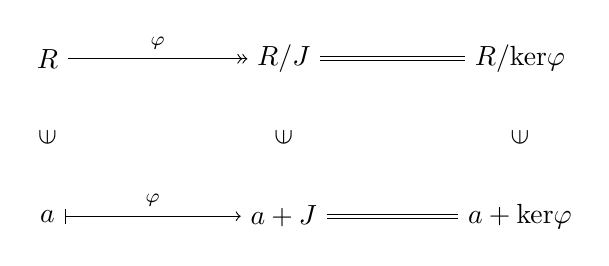
\begin{tikzpicture}[auto]
    \node[rotate=90] (a) at (0, 1) {$\in $};
    \node[rotate=90] (b) at (3, 1) {$\in $};
    \node[rotate=90] (c) at (6, 1) {$\in $};
    \node (a) at (0, 2) {$R$};
    \node (b) at (3, 2) {$R/J$};
    \node (c) at (6, 2) {$R/{\rm ker} \varphi $};
    \draw [->>] (a) to node {$\scriptstyle \varphi $} (b);
    \draw [double distance=1pt] (b) to node {$\scriptstyle $} (c);
    \node (a) at (0, 0) {$a$};
    \node (b) at (3, 0) {$a+J$};
    \node (c) at (6, 0) {$a+{\rm ker} \varphi $};
    \draw [|->] (a) to node {$\scriptstyle \varphi $} (b);
    \draw [double distance=1pt] (b) to node {$\scriptstyle $} (c);
  \end{tikzpicture}
\end{center}
\end{dfn}
\begin{proof}
環$R$のideal$J$が与えられたとき、写像$\varphi:R \rightarrow {R}/{J};a \mapsto a + J$について、$\forall a,b \in R$に対し、次のようになる。
\begin{align*}
\varphi(a + b) &= (a + b) + J\\
&= (a + J) + (b + J)\\
&= \varphi(a) + \varphi(b)\\
\varphi(ab) &= ab + J\\
&= (a + J)(b + J)\\
&= \varphi(a)\varphi(b)\\
\varphi(1) &= 1 + J
\end{align*}
これにより、その写像$\varphi$は環準同型写像である。\par
また、その商環${R}/{J}$の零元は$J$であるので、$\forall a \in \ker\varphi$に対し、次のようになる。
\begin{align*}
\varphi(a) = a + J = J
\end{align*}
ここで、$\forall b \in J$に対し、$b = a + b'$なる元$b'$がそのideal$J$に存在し次のようになるので、
\begin{align*}
a &= a + 0\\
&= a + b' - b'\\
&= b - b' \in J
\end{align*}
$a \in J$が成り立つ。逆に、$\forall a \in J$が成り立つなら、次のようになるので、
\begin{align*}
\varphi(a) &= a + J\\
&= \left\{ a + b \in R \middle| b \in J \right\}\\
&= \left\{ a + b \in R \middle| a + b \in J \right\}\\
&= J
\end{align*}
$a \in \ker\varphi$が成り立つ。以上より、$\ker\varphi = J$が得られる。\par
最後に、$\forall a + J \in {R}/{J}$に対し、商環の定義より明らかに$\varphi(a) = a + J$なるその環$R$の元$a$が存在するので、その写像$\varphi$は全射である。これにより、その写像$\varphi$は全射環準同型写像である。
\end{proof}
%\hypertarget{ux74b0ux6e96ux540cux578bux5b9aux7406}{%
\subsubsection{環準同型定理}%\label{ux74b0ux6e96ux540cux578bux5b9aux7406}}
\begin{thm}\label{3.3.2.20}
2つの環々$R$、$S$の間の環準同型写像$f:R \rightarrow S$が与えられたとき、その環$R$が斜体でそれらの環々$R$、$S$が零環でないなら、その写像$f$は単射環準同型写像である。
\end{thm}
\begin{proof}
2つの環々$R$、$S$の間の環準同型写像$f:R \rightarrow S$が与えられたとき、その環$R$が斜体でそれらの環々$R$、$S$が零環でないなら、その環$R$のidealは定理\ref{3.3.2.4}より零idealかその環$R$自身しかもたないことになる。ここで、その環$S$が零環でないので、その核$\ker f$はその環$R$自身になりえないので、その核$\ker f$は零idealであることになる。このとき、$\forall f(a),f(b) \in V(f)$に対し、$f(a) = f(b)$が成り立つなら、その環$S$の零元を$0_{S}$として次のようになり、
\begin{align*}
f(a) = f(b) &\Leftrightarrow f(a) - f(b) = f(a) + f( - b) = f(a - b) = 0_{S}\\
&\Leftrightarrow a - b \in \ker f\\
&\Leftrightarrow a - b \in R0\\
&\Leftrightarrow a - b = 0\\
&\Leftrightarrow a = b
\end{align*}
その写像$f$は単射である。よって、その環$R$が斜体でそれらの環々$R$、$S$が零環でないなら、その写像$f$は単射環準同型写像である。
\end{proof}
\begin{thm}[環準同型定理]\label{3.3.2.21}
2つの環々$R$、$S$の間の環準同型写像$f:R \rightarrow S$の核$\ker f$が与えられたとき、その環$R$からその商環${R}/{\ker f}$への自然な全射環準同型写像を$\varphi$とおいた次式のような写像$g$は環同型写像である。
\begin{center}
  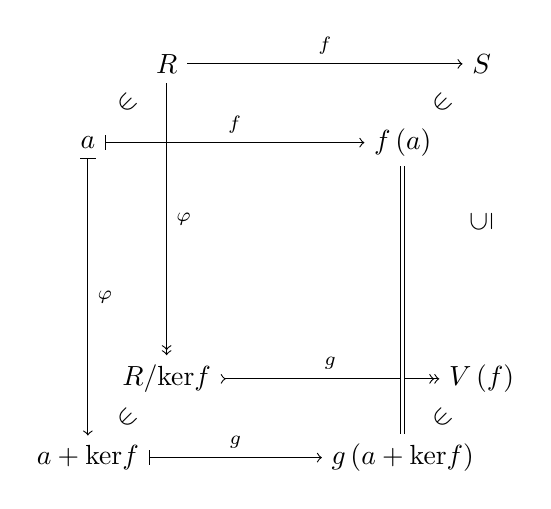
\begin{tikzpicture}[auto]
    \node (a) at (0, 0) {$a+{\rm ker} f$};
    \node (b) at (4, 0) {$g\left( a+{\rm ker} f\right) $};
    \node (c) at (0, 4) {$a$};
    \node (d) at (4, 4) {$f\left( a\right) $};
    \node (e) at (1, 1) {$R/{\rm ker} f$};
    \node (f) at (5, 1) {$V\left( f\right) $};
    \node (g) at (1, 5) {$R$};
    \node (h) at (5, 5) {$S$};
    \node[rotate=45] (i) at (0.5, 0.5) {$\in $};
    \node[rotate=45] (j) at (4.5, 0.5) {$\in $};
    \node[rotate=45] (k) at (0.5, 4.5) {$\in $};
    \node[rotate=45] (l) at (4.5, 4.5) {$\in $};
    \node[rotate=90] (m) at (5, 3) {$\subseteq $};
    \draw [|->] (a) to node {$\scriptstyle g$} (b);
    \draw [>->>] (e) to node {$\scriptstyle g$} (f);
    \draw [|->] (c) to node {$\scriptstyle \varphi $} (a);
    \draw [->>] (g) to node {$\scriptstyle \varphi $} (e);
    \draw [|->] (c) to node {$\scriptstyle f$} (d);
    \draw [->] (g) to node {$\scriptstyle f$} (h);
    \draw [double distance=1pt] (b) to node {$ $} (d);
  \end{tikzpicture} 
\end{center}
これにより、${R}/{\ker f} \cong V(f)$が成り立つ。\par
この定理を環準同型定理という。
\end{thm}
\begin{proof}
2つの環々$R$、$S$の間の環準同型写像$f:R \rightarrow S$の核$\ker f$が与えられたとき、その環$R$からその商環${R}/{\ker f}$への自然な全射環準同型写像を$\varphi$とおいた次式のような写像$g$について、
\begin{center}
  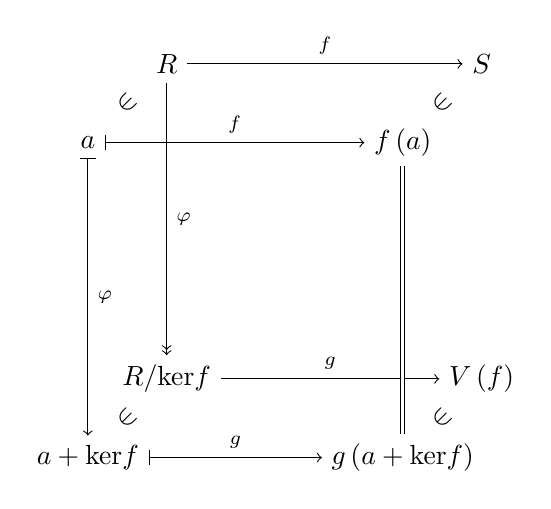
\begin{tikzpicture}[auto]
    \node (a) at (0, 0) {$a+{\rm ker} f$};
    \node (b) at (4, 0) {$g\left( a+{\rm ker} f\right) $};
    \node (c) at (0, 4) {$a$};
    \node (d) at (4, 4) {$f\left( a\right) $};
    \node (e) at (1, 1) {$R/{\rm ker} f$};
    \node (f) at (5, 1) {$V\left( f\right) $};
    \node (g) at (1, 5) {$R$};
    \node (h) at (5, 5) {$S$};
    \node[rotate=45] (i) at (0.5, 0.5) {$\in $};
    \node[rotate=45] (j) at (4.5, 0.5) {$\in $};
    \node[rotate=45] (k) at (0.5, 4.5) {$\in $};
    \node[rotate=45] (l) at (4.5, 4.5) {$\in $};
    \draw [|->] (a) to node {$\scriptstyle g$} (b);
    \draw [->] (e) to node {$\scriptstyle g$} (f);
    \draw [|->] (c) to node {$\scriptstyle \varphi $} (a);
    \draw [->>] (g) to node {$\scriptstyle \varphi $} (e);
    \draw [|->] (c) to node {$\scriptstyle f$} (d);
    \draw [->] (g) to node {$\scriptstyle f$} (h);
    \draw [double distance=1pt] (b) to node {$ $} (d);
  \end{tikzpicture}
\end{center}
この環$R$の単位元を$1_{R}$、この環$S$の零元を$0_{S}$、単位元を$1_{S}$とおくと、その値域の定義より明らかにその写像$g$は全射である。また、$g\left( a + \ker f \right) = g\left( b + \ker f \right)$が成り立つなら、その核$\ker f$はその環$R$のidealであることにより次のようになる。
\begin{align*}
g\left( a + \ker f \right) = g\left( b + \ker f \right) &\Leftrightarrow f(a) = f(b)\\
&\Leftrightarrow f(a) - f(b) = 0_{S}\\
&\Leftrightarrow f(a) + f( - b) = 0_{S}\\
&\Leftrightarrow f(a - b) = 0_{S}\\
&\Leftrightarrow a - b \in \ker f\\
&\Leftrightarrow b - a \in \ker f
\end{align*}
ここで、$b - a \in \ker f$が成り立つなら、$a \equiv b\ \left( \mathrm{mod}{\ker f} \right)$が成り立ち、したがって、$a + \ker f = b + \ker f$が成り立つので、その写像$g$は単射である。以上より、その写像$g$は全単射である。\par
その組$\left( \ker f, + \right)$は群をなすのであったので、$\forall a + \ker f,b + \ker f \in {R}/{\ker f}$に対し、次のようになる。
\begin{align*}
g\left( \left( a + \ker f \right) + \left( b + \ker f \right) \right) &= g\left( (a + b) + \ker f \right)\\
&= f(a + b)\\
&= f(a) + f(b)\\
&= g\left( a + \ker f \right) + g\left( b + \ker f \right)\\
g\left( \left( a + \ker f \right)\left( b + \ker f \right) \right) &= g\left( ab + \ker f \right)\\
&= f(ab)\\
&= f(a)f(b)\\
&= g\left( a + \ker f \right)g\left( b + \ker f \right)\\
g\left( 1_{R} + \ker f \right) &= f\left( 1_{R} \right) = 1_{S}
\end{align*}
これにより、その写像$g$は環準同型写像であり、その写像$g$は全単射だったので、その写像$g$は環同型写像である。\par
これにより、2つのそれらの環々${R}/{\ker f}$、$V(f)$は、その環${R}/{\ker f}$からその環$V(f)$への環同型写像$g:{R}/{\ker f} \rightarrow V(f)$が存在するので、環同型である、即ち、${R}/{\ker f} \cong V(f)$が成り立つ。
\end{proof}
%\hypertarget{ux74b0ux540cux578bux5b9aux7406}{%
\subsubsection{環同型定理}%\label{ux74b0ux540cux578bux5b9aux7406}}
\begin{thm}\label{3.3.2.22}
2つの環々$R$、$S$の間の全射環準同型写像$f:R \twoheadrightarrow S$について、その環$R$の左ideal$I$、右ideal$J$を用いた2つの集合たち$V\left( f|I \right)$、$V\left( f|J \right)$はそれぞれその環$S$の左ideal、右idealである。また、その環$S$の左ideal$I$、右ideal$J$を用いた2つの集合たち$V\left( f^{- 1}|I \right)$、$V\left( f^{- 1}|J \right)$はそれぞれその環$R$の左ideal、右idealである。
\end{thm}
\begin{proof}
2つの環々$R$、$S$の間の全射環準同型写像$f:R \twoheadrightarrow S$について、その環$R$の左ideal$I$が与えられたとき、$\forall f(a),\ f(b) \in V\left( f|I \right)$に対し、定義より$a + b \in I$も成り立つので、次のようになる。
\begin{align*}
f(a) + f(b) = f(a + b) \in V\left( f|I \right)
\end{align*}
$\forall f(a) \in V\left( f|I \right)\forall s \in S$に対し、その写像$f$は全射であるから、$\exists r \in R$に対し、$f(r) = s$が成り立ち、定義より$ra \in I$も成り立つので、次のようになる。
\begin{align*}
sf(a) &= f(r)f(a)\\
&= f(ra)\\
&= f(ra) \in V\left( f|I \right)
\end{align*}
したがって、集合$V\left( f|I \right)$はその環$S$の左idealである。同様にして、その環$R$の右ideal$J$が与えられたとき、集合$V\left( f|J \right)$はその環$S$の右idealであることが示される。\par
また、その環$S$の左ideal$I$が与えられたとき、環準同型写像の定義と左idealの定義より、$\forall a,b \in V\left( f^{- 1}|I \right)$に対し、次のようになる。
\begin{align*}
a,b \in V\left( f^{- 1}|I \right) &\Rightarrow f(a),f(b) \in V\left( f|V\left( f^{- 1}|I \right) \right) \subseteq I\\
&\Rightarrow f(a) + f(b) = f(a + b) \in I\\
&\Rightarrow a + b \in V\left( f^{- 1}|I \right)
\end{align*}
$f( - a) = - f(a)$が成り立つことと左idealの定義より、$\forall a \in V\left( f^{- 1}|I \right)\forall r \in R$に対し、次のようになる。
\begin{align*}
a \in V\left( f^{- 1}|I \right) &\Rightarrow f(a) \in V\left( f|V\left( f^{- 1}|I \right) \right) \subseteq I\\
&\Rightarrow f(r)f(a) = f(ra) \in I\\
&\Rightarrow ra \in V\left( f^{- 1}|I \right)
\end{align*}
したがって、集合$V\left( f^{- 1}|I \right)$はその環$R$の左idealである。同様にして、その環$S$の右ideal$J$が与えられたとき、集合$V\left( f^{- 1}|J \right)$はその環$R$の右idealであることが示される。
\end{proof}
\begin{thm}[環同型定理]\label{3.3.2.23}
2つの環々$R$、$S$の間の全射環準同型写像$f:R \twoheadrightarrow S$について、その核$\ker f$を含むその環$R$の左ideal全体の集合を$\mathfrak{I}_{R}'$、その環$S$の左ideal全体の集合を$\mathfrak{I}_{S}$とおくと、次のことが成り立つ。右idealについても同様である。この定理を環同型定理という。
\begin{itemize}
\item
  次式のように写像$F:\mathfrak{I}_{R}' \rightarrow \mathfrak{I}_{S};I \mapsto V\left( f|I \right) = J$は全単射でその逆写像$F^{- 1}$が$F^{- 1}:\mathfrak{I}_{S} \rightarrow \mathfrak{I}_{R}';J \mapsto V\left( f^{- 1}|J \right) = I$と与えられる。これは次式のようにも表される。
\begin{center}
  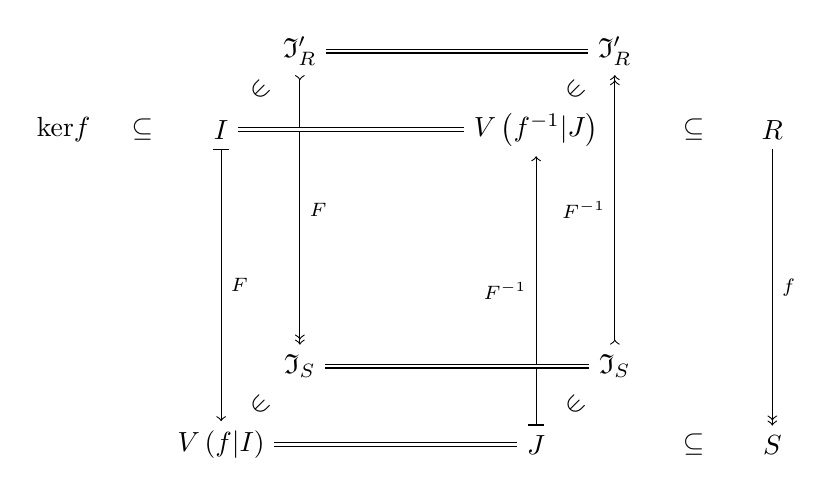
\begin{tikzpicture}[auto]
    \node[rotate=45] (x) at (2.5, 4.5) {$\in $};
    \node[rotate=45] (x) at (2.5, 0.5) {$\in $};
    \node[rotate=45] (x) at (6.5, 0.5) {$\in $};
    \node[rotate=45] (x) at (6.5, 4.5) {$\in $};
    \node (y) at (1, 4) {$\subseteq $};
    \node (y) at (8, 4) {$\subseteq $};
    \node (y) at (8, 0) {$\subseteq $};
    \node (a) at (3, 5) {${\mathfrak I}_R' $};
    \node (b) at (3, 1) {${\mathfrak I}_S $};
    \node (c) at (2, 4) {$I$};
    \node (d) at (2, 0) {$V\left( f|I\right) $};
    \node (e) at (6, 0) {$J$};
    \node (f) at (6, 4) {$V\left( f^{-1} |J\right) $};
    \node (g) at (7, 1) {${\mathfrak I}_S $};
    \node (h) at (7, 5) {${\mathfrak I}_R' $};
    \node (i) at (9, 4) {$R$};
    \node (j) at (9, 0) {$S$};
    \node (k) at (0, 4) {${\rm ker} f$};
    \draw [>->>] (a) to node {$\scriptstyle F$} (b);
    \draw [|->] (c) to node {$\scriptstyle F$} (d);
    \draw [>->>] (g) to node {$\scriptstyle F^{-1} $} (h);
    \draw [|->] (e) to node {$\scriptstyle F^{-1} $} (f);
    \draw [->>] (i) to node {$\scriptstyle f$} (j);
    \draw [double distance=1pt] (c) to node {} (f);
    \draw [double distance=1pt] (d) to node {} (e);
    \draw [double distance=1pt] (a) to node {} (h);
    \draw [double distance=1pt] (b) to node {} (g);
  \end{tikzpicture}
\end{center}
\item
  $\forall I \in \mathfrak{I}_{R}'$に対し、$F(I) = V\left( f|I \right) = J$とおくと、次式のようになり、さらに、${I}/{\ker f} \cong J$が成り立つ。
\begin{center}
  \begin{tikzpicture}[auto]
    \node[rotate=45] (x) at (2.5, 4.5) {$\in $};
    \node[rotate=45] (x) at (2.5, 0.5) {$\in $};
    \node (y) at (1, 4) {$\subseteq $};
    \node (y) at (7, 4) {$\subseteq $};
    \node (y) at (7, 0) {$\subseteq $};
    \node (a) at (3, 5) {${\mathfrak I}_R' $};
    \node (b) at (3, 1) {${\mathfrak I}_S $};
    \node (c) at (2, 4) {$I$};
    \node (d) at (2, 0) {$V\left( f|J\right) $};
    \node (e) at (6, 0) {$J$};
    \node (f) at (12, 4) {$I/{\rm ker} f$};
    \node (i) at (8, 4) {$R$};
    \node (j) at (8, 0) {$S$};
    \node (k) at (0, 4) {${\rm ker} f$};
    \draw [>->>] (a) to node {$\scriptstyle F$} (b);
    \draw [|->] (c) to node {$\scriptstyle F$} (d);
    \draw [>->>] (f) to node {} (e);
    \draw [->>] (i) to node {$\scriptstyle f$} (j);
    \draw [double distance=1pt] (d) to node {} (e);
    \draw [->>] (c)[bend left=10] to node {} (f);
  \end{tikzpicture}
\end{center}
\item
  $\forall I \in \mathfrak{I}_{R}'$に対し、その写像$F:\mathfrak{I}_{R}' \rightarrow \mathfrak{I}_{S};I \mapsto V\left( f|I \right)$が与えられたとき、$F(I) = V\left( f|I \right) = J$とおくと、その左ideal$I$がその環$R$のidealであるならそのときに限り、その左ideal$J$がその環$S$のidealである。
\item
  $\forall I \in \mathfrak{I}_{R}'$に対し、その写像$F:\mathfrak{I}_{R}' \rightarrow \mathfrak{I}_{S};I \mapsto V\left( f|I \right)$が与えられたとき、$F(I) = V\left( f|I \right) = J$とおくと、その左ideal$I$がその環$R$のidealであるなら、次式のようになり、さらに、${R}/{I} \cong {S}/{J}$が成り立つ。
\begin{center}
  \begin{tikzpicture}[auto]
    \node[rotate=45] (x) at (2.5, 4.5) {$\in $};
    \node[rotate=45] (x) at (2.5, 0.5) {$\in $};
    \node (y) at (1, 4) {$\subseteq $};
    \node (y) at (7, 4) {$\subseteq $};
    \node (y) at (7, 0) {$\subseteq $};
    \node (a) at (3, 5) {${\mathfrak I}_R' $};
    \node (b) at (3, 1) {${\mathfrak I}_S $};
    \node (c) at (2, 4) {$I$};
    \node (d) at (2, 0) {$V\left( f|I\right) $};
    \node (e) at (6, 0) {$J$};
    \node (g) at (12, 0) {$S/J$};
    \node (h) at (12, 4) {$R/I$};
    \node (i) at (8, 4) {$R$};
    \node (j) at (8, 0) {$S$};
    \node (k) at (0, 4) {${\rm ker} f$};
    \draw [>->>] (a) to node {$\scriptstyle F$} (b);
    \draw [|->] (c) to node {$\scriptstyle F$} (d);
    \draw [>->>] (h) to node {} (g);
    \draw [->>] (i) to node {$\scriptstyle f$} (j);
    \draw [double distance=1pt] (d) to node {} (e);
    \draw [->>] (i) to node {} (h);
    \draw [->>] (j) to node {} (g);
  \end{tikzpicture} 
\end{center}
\end{itemize}
\end{thm}
\begin{proof}
2つの環々$R$、$S$の間の全射環準同型写像$f:R \twoheadrightarrow S$について、その核$\ker f$を含むその環$R$の左ideal全体の集合を$\mathfrak{I}_{R}'$、その環$S$の左ideal全体の集合を$\mathfrak{I}_{S}$とおきその環$S$の零元を$0_{S}$とおく。次式のように写像$F:\mathfrak{I}_{R}' \rightarrow \mathfrak{I}_{S};I \mapsto V\left( f|I \right) = J$を考えよう。
\begin{center}
  \begin{tikzpicture}[auto]
    \node[rotate=45] (x) at (2.5, 4.5) {$\in $};
    \node[rotate=45] (x) at (2.5, 0.5) {$\in $};
    \node (y) at (1, 4) {$\subseteq $};
    \node (y) at (7, 4) {$\subseteq $};
    \node (y) at (7, 0) {$\subseteq $};
    \node (a) at (3, 5) {${\mathfrak I}_R' $};
    \node (b) at (3, 1) {${\mathfrak I}_S $};
    \node (c) at (2, 4) {$I$};
    \node (d) at (2, 0) {$V\left( f|I\right) $};
    \node (e) at (6, 0) {$J$};
    \node (i) at (8, 4) {$R$};
    \node (j) at (8, 0) {$S$};
    \node (k) at (0, 4) {${\rm ker} f$};
    \draw [->] (a) to node {$\scriptstyle F$} (b);
    \draw [|->] (c) to node {$\scriptstyle F$} (d);
    \draw [->>] (i) to node {$\scriptstyle f$} (j);
    \draw [double distance=1pt] (d) to node {} (e);
  \end{tikzpicture} 
\end{center}
$\forall I \in \mathfrak{I}_{R}'$に対し、定理\ref{3.3.2.22}よりその集合$V\left( f|I \right)$はその環$S$の左idealであるので、$V\left( f|I \right) \in \mathfrak{I}_{S}$が成り立つ。したがって、写像$F:\mathfrak{I}_{R}' \rightarrow \mathfrak{I}_{S};I \mapsto V\left( f|I \right)$が定義できている。ここで、次式のように写像$G:\mathfrak{I}_{S} \rightarrow \mathfrak{I}_{R}';J \mapsto V\left( f^{- 1}|J \right) = I$を考えよう。
\begin{center}
  \begin{tikzpicture}[auto]
    \node[rotate=45] (x) at (2.5, 4.5) {$\in $};
    \node[rotate=45] (x) at (2.5, 0.5) {$\in $};
    \node[rotate=45] (x) at (6.5, 0.5) {$\in $};
    \node[rotate=45] (x) at (6.5, 4.5) {$\in $};
    \node (y) at (1, 4) {$\subseteq $};
    \node (y) at (8, 4) {$\subseteq $};
    \node (y) at (8, 0) {$\subseteq $};
    \node (a) at (3, 5) {${\mathfrak I}_R' $};
    \node (b) at (3, 1) {${\mathfrak I}_S $};
    \node (c) at (2, 4) {$I$};
    \node (d) at (2, 0) {$V\left( f|I\right) $};
    \node (e) at (6, 0) {$J$};
    \node (f) at (6, 4) {$V\left( f^{-1} |J\right) $};
    \node (g) at (7, 1) {${\mathfrak I}_S $};
    \node (h) at (7, 5) {${\mathfrak I}_R' $};
    \node (i) at (9, 4) {$R$};
    \node (j) at (9, 0) {$S$};
    \node (k) at (0, 4) {${\rm ker} f$};
    \draw [->] (a) to node {$\scriptstyle F$} (b);
    \draw [|->] (c) to node {$\scriptstyle F$} (d);
    \draw [->] (g) to node {$\scriptstyle G$} (h);
    \draw [|->] (e) to node {$\scriptstyle G$} (f);
    \draw [->>] (i) to node {$\scriptstyle f$} (j);
    \draw [double distance=1pt] (d) to node {} (e);
    \draw [double distance=1pt] (a) to node {} (h);
    \draw [double distance=1pt] (b) to node {} (g);
  \end{tikzpicture} 
\end{center}
$\forall J \in \mathfrak{I}_{S}$に対し、定理\ref{3.3.2.22}よりその集合$V\left( f^{- 1}|J \right)$はその環$R$の左idealであるかつ、$\forall a \in J$に対し、$- a \in J$が成り立ち、したがって、$a - a = 0_{S} \in J$が成り立つことから、$\ker f = V\left( f^{- 1}|\left\{ 0_{S} \right\} \right) \subseteq V\left( f^{- 1}|J \right)$が成り立つので、$V\left( f^{- 1}|J \right) \in \mathfrak{I}_{R}'$が成り立つ。したがって、写像$G:\mathfrak{I}_{S} \rightarrow \mathfrak{I}_{R}';J \mapsto V\left( f^{- 1}|J \right)$が定義できている。\par
まず、$G \circ F = I_{\mathfrak{I}_{R}'}$が成り立つことを示そう。このとき、$\forall I \in \mathfrak{I}_{R}'$に対し、$V\left( f^{- 1}|V\left( f|I \right) \right) \supseteq I$は明らかに成り立つ。逆に、$\forall a \in R$に対し、$a \in V\left( f^{- 1}|V\left( f|I \right) \right)$が成り立つなら、$V\left( f|V\left( f^{- 1}|V\left( f|I \right) \right) \right) = V\left( f|I \right)$が成り立つので、$f(a) \in V\left( f|I \right)$が成り立ち、$\exists a \in I$に対し、$f(a) = f(b)$が成り立つ。したがって、次のようになり、
\begin{align*}
f(a) = f(b) &\Leftrightarrow f(a) - f(b) = f(a) + f( - b) = f(a - b) = 0_{S}\\
&\Leftrightarrow a - b \in \ker f
\end{align*}
したがって、次のようになる。
\begin{align*}
(a - b) + b &= a + 0\\
&= a \in I
\end{align*}
以上より、$V\left( f^{- 1}|V\left( f|I \right) \right) \subseteq I$が成り立つ。したがって、$G \circ F(I) = V\left( f^{- 1}|V\left( f|I \right) \right) = I$が成り立つので、$G \circ F = I_{\mathfrak{I}_{R}'}$が得られた。\par
次に、$F \circ G = I_{\mathfrak{I}_{S}}$が成り立つことを示そう。もちろん、$\forall J \in \mathfrak{I}_{S}$に対し、$V\left( f|V\left( f^{- 1}|J \right) \right) \subseteq J$は成り立つ。逆に、$\forall a \in S$に対し、$a \in J$が成り立つなら、その写像$f$は全射であるので、$\exists b \in R$に対し、$f(b) = a$が成り立つ。$a \in J$より$V\left( f^{- 1}|\left\{ a \right\} \right) \subseteq V\left( f^{- 1}|J \right)$が成り立つので、$b \in V\left( f^{- 1}|\left\{ a \right\} \right) \subseteq V\left( f^{- 1}|J \right)$が成り立ち、したがって、$f(b) = a \in V\left( f|V\left( f^{- 1}|J \right) \right)$が成り立つ。以上より、$J \subseteq V\left( f|V\left( f^{- 1}|J \right) \right)$が成り立つ。したがって、$F \circ G(J) = V\left( f|V\left( f^{- 1}|J \right) \right) = J$が成り立つので、$F \circ G = I_{\mathfrak{I}_{S}}$が得られた。\par
以上より、$G \circ F = I_{\mathfrak{I}_{R}'}$かつ$F \circ G = I_{\mathfrak{I}_{S}}$が成り立つ。このようなその写像$G:\mathfrak{I}_{S} \rightarrow \mathfrak{I}_{R}'$が存在するので、その写像$F:\mathfrak{I}_{R}' \rightarrow \mathfrak{I}_{S}$は全単射でその写像$G$はその写像$F$の逆写像である。よって、その写像$F:\mathfrak{I}_{R}' \rightarrow \mathfrak{I}_{S};I \mapsto V\left( f|I \right) = J$は全単射でその逆写像$F^{- 1}$が$F^{- 1}:\mathfrak{I}_{S} \rightarrow \mathfrak{I}_{R}';J \mapsto V\left( f^{- 1}|J \right) = I$と与えられる。\par
また、$\forall I \in \mathfrak{I}_{R}'$に対し、写像$f':I \rightarrow V\left( f|I \right);a \mapsto f(a)$を考え$F(I) = V\left( f|I \right) = J$とおくと、この写像$f'$は明らかに全射環準同型写像であるから、次式のように考えられると、
\begin{center}
  \begin{tikzpicture}[auto]
    \node[rotate=45] (x) at (2.5, 4.5) {$\in $};
    \node[rotate=45] (x) at (2.5, 0.5) {$\in $};
    \node[rotate=45] (x) at (6.5, 4.5) {$\in $};
    \node (a) at (3, 5) {$I$};
    \node (b) at (3, 1) {$I/{\rm ker} f' $};
    \node (c) at (2, 4) {$a$};
    \node (d) at (2, 0) {$a+{\rm ker} f' $};
    \node (f) at (6, 4) {$f\left( a\right) $};
    \node (g) at (7, 1) {$V\left( f'|I\right) $};
    \node (h) at (7, 5) {$J$};
    \draw [->>] (a) to node {} (b);
    \draw [|->] (c) to node {} (d);
    \draw [->>] (a) to node {$\scriptstyle f'$} (h);
    \draw [|->] (c) to node {$\scriptstyle f'$} (f);
    \draw [double distance=1pt] (g) to node {} (h);
  \end{tikzpicture} 
\end{center}
環準同型定理より次式が成り立つので、
\begin{center}
  \begin{tikzpicture}[auto]
    \node[rotate=45] (x) at (2.5, 4.5) {$\in $};
    \node[rotate=45] (x) at (2.5, 0.5) {$\in $};
    \node[rotate=45] (x) at (6.5, 4.5) {$\in $};
    \node (a) at (3, 5) {$I$};
    \node (b) at (3, 1) {$I/{\rm ker} f' $};
    \node (c) at (2, 4) {$a$};
    \node (d) at (2, 0) {$a+{\rm ker} f' $};
    \node (f) at (6, 4) {$f\left( a\right) $};
    \node (g) at (7, 1) {$V\left( f'|I\right) $};
    \node (h) at (7, 5) {$J$};
    \draw [->>] (a) to node {} (b);
    \draw [|->] (c) to node {} (d);
    \draw [->>] (a) to node {$\scriptstyle f'$} (h);
    \draw [|->] (c) to node {$\scriptstyle f'$} (f);
    \draw [double distance=1pt] (g) to node {} (h);
    \draw [>->>] (b) to node {} (g);
  \end{tikzpicture} 
\end{center}
次式のようになり、
\begin{center}
  \begin{tikzpicture}[auto]
    \node[rotate=45] (x) at (2.5, 4.5) {$\in $};
    \node[rotate=45] (x) at (2.5, 0.5) {$\in $};
    \node (y) at (1, 4) {$\subseteq $};
    \node (y) at (7, 4) {$\subseteq $};
    \node (y) at (7, 0) {$\subseteq $};
    \node (a) at (3, 5) {${\mathfrak I}_R' $};
    \node (b) at (3, 1) {${\mathfrak I}_S $};
    \node (c) at (2, 4) {$I$};
    \node (d) at (2, 0) {$V\left( f|I\right) $};
    \node (e) at (6, 0) {$J$};
    \node (f) at (12, 4) {$I/{\rm ker} f'$};
    \node (i) at (8, 4) {$R$};
    \node (j) at (8, 0) {$S$};
    \node (k) at (0, 4) {${\rm ker} f$};
    \node (l) at (12, 0) {$V\left( f'|I\right) $};
    \draw [>->>] (a) to node {$\scriptstyle F$} (b);
    \draw [|->] (c) to node {$\scriptstyle F$} (d);
    \draw [>->>] (f) to node {} (l);
    \draw [->>] (i) to node {$\scriptstyle f$} (j);
    \draw [double distance=1pt] (d) to node {} (e);
    \draw [->>] (c)[bend left=10] to node {} (f);
  \end{tikzpicture} 
\end{center}
${I}/{\ker f'} \cong V\left( f'|I \right)$が得られる。ここで、$V\left( f'|I \right) = V\left( f|I \right) = J$が成り立つかつ、$\ker f' = \ker f$が成り立つので、次式のようになり、
\begin{center}
  \begin{tikzpicture}[auto]
    \node[rotate=45] (x) at (2.5, 4.5) {$\in $};
    \node[rotate=45] (x) at (2.5, 0.5) {$\in $};
    \node (y) at (1, 4) {$\subseteq $};
    \node (y) at (7, 4) {$\subseteq $};
    \node (y) at (7, 0) {$\subseteq $};
    \node (a) at (3, 5) {${\mathfrak I}_R' $};
    \node (b) at (3, 1) {${\mathfrak I}_S $};
    \node (c) at (2, 4) {$I$};
    \node (d) at (2, 0) {$V\left( f|J\right) $};
    \node (e) at (6, 0) {$J$};
    \node (f) at (12, 4) {$I/{\rm ker} f$};
    \node (i) at (8, 4) {$R$};
    \node (j) at (8, 0) {$S$};
    \node (k) at (0, 4) {${\rm ker} f$};
    \draw [>->>] (a) to node {$\scriptstyle F$} (b);
    \draw [|->] (c) to node {$\scriptstyle F$} (d);
    \draw [>->>] (f) to node {} (e);
    \draw [->>] (i) to node {$\scriptstyle f$} (j);
    \draw [double distance=1pt] (d) to node {} (e);
    \draw [->>] (c)[bend left=10] to node {} (f);
  \end{tikzpicture}
\end{center}
${I}/{\ker f} \cong J$が成り立つ。\par
$\forall I \in \mathfrak{I}_{R}'$に対し、その写像$F:\mathfrak{I}_{R}' \rightarrow \mathfrak{I}_{S};I \mapsto V\left( f|I \right)$が与えられたとき、$F(I) = V\left( f|I \right) = J$とおくと、定理\ref{3.3.2.22}よりその左ideal$I$がその環$R$のidealであるならそのときに限り、その左ideal$J$がその環$S$のidealであることが直ちに分かる。\par
$\forall I \in \mathfrak{I}_{R}'$に対し、その写像$F:\mathfrak{I}_{R}' \rightarrow \mathfrak{I}_{S};I \mapsto V\left( f|I \right)$が与えられたとき、$F(I) = V\left( f|I \right) = J$とおくと、その左ideal$I$がその環$R$のidealであるなら、上記の議論により集合$J$はその環$S$のidealで次式のように自然な全射環準同型写像$\varphi_{S}:S \twoheadrightarrow {S}/{J}$を考えると、
\begin{center}
  \begin{tikzpicture}[auto]
    \node[rotate=45] (x) at (2.5, 4.5) {$\in $};
    \node[rotate=45] (x) at (2.5, 0.5) {$\in $};
    \node (y) at (1, 4) {$\subseteq $};
    \node (y) at (7, 4) {$\subseteq $};
    \node (y) at (7, 0) {$\subseteq $};
    \node (a) at (3, 5) {${\mathfrak I}_R' $};
    \node (b) at (3, 1) {${\mathfrak I}_S $};
    \node (c) at (2, 4) {$I$};
    \node (d) at (2, 0) {$V\left( f|I\right) $};
    \node (e) at (6, 0) {$J$};
    \node (g) at (12, 0) {$S/J$};
    \node (i) at (8, 4) {$R$};
    \node (j) at (8, 0) {$S$};
    \node (k) at (0, 4) {${\rm ker} f$};
    \draw [>->>] (a) to node {$\scriptstyle F$} (b);
    \draw [|->] (c) to node {$\scriptstyle F$} (d);
    \draw [->>] (i) to node {$\scriptstyle f$} (j);
    \draw [double distance=1pt] (d) to node {} (e);
    \draw [->>] (j) to node {$\scriptstyle \varphi_S $} (g);
  \end{tikzpicture} 
\end{center}
$J = \ker\varphi_{S}$が成り立ち、$\varphi_{S} \circ f = \rho$とおくと、その写像$\rho$は次式のように全射環準同型写像で、
\begin{center}
  \begin{tikzpicture}[auto]
    \node[rotate=45] (x) at (2.5, 4.5) {$\in $};
    \node[rotate=45] (x) at (2.5, 0.5) {$\in $};
    \node (y) at (1, 4) {$\subseteq $};
    \node (y) at (7, 4) {$\subseteq $};
    \node (y) at (7, 0) {$\subseteq $};
    \node (a) at (3, 5) {${\mathfrak I}_R' $};
    \node (b) at (3, 1) {${\mathfrak I}_S $};
    \node (c) at (2, 4) {$I$};
    \node (d) at (2, 0) {$V\left( f|I\right) $};
    \node (e) at (6, 0) {$J$};
    \node (g) at (12, 0) {$S/J$};
    \node (i) at (8, 4) {$R$};
    \node (j) at (8, 0) {$S$};
    \node (k) at (0, 4) {${\rm ker} f$};
    \draw [>->>] (a) to node {$\scriptstyle F$} (b);
    \draw [|->] (c) to node {$\scriptstyle F$} (d);
    \draw [->>] (i) to node {$\scriptstyle f$} (j);
    \draw [double distance=1pt] (d) to node {} (e);
    \draw [->>] (j) to node {$\scriptstyle \varphi_S $} (g);
    \draw [->>] (i) to node {$\scriptstyle \rho $} (g);
  \end{tikzpicture} 
\end{center}
$\forall a \in R$に対し、$a \in \ker\rho$が成り立つならそのときに限り、$\rho(a) = f(a) + J = J$が成り立ち、これが成り立つならそのときに限り、$f(a) \in J$が成り立つ、即ち、$a \in V\left( f^{- 1}|J \right)$が成り立つ。ここで、上記の議論により$a \in F^{- 1}(J) = I$が成り立つので、$\ker\rho = I$が得られる。以上より、自然な全射環準同型写像$\varphi_{R}:R \twoheadrightarrow {R}/{\ker\rho}$を用いれば、次式のように与えられ、
\begin{center}
  \begin{tikzpicture}[auto]
    \node[rotate=45] (x) at (2.5, 4.5) {$\in $};
    \node[rotate=45] (x) at (2.5, 0.5) {$\in $};
    \node[rotate=45] (x) at (6.5, 4.5) {$\in $};
    \node (a) at (3, 5) {$R$};
    \node (b) at (3, 1) {$R/{\rm ker} \rho $};
    \node (c) at (2, 4) {$a$};
    \node (d) at (2, 0) {$a+{\rm ker} \rho $};
    \node (f) at (6, 4) {$f\left( a\right) +J$};
    \node (g) at (7, 1) {$V\left( \rho \right) $};
    \node (h) at (7, 5) {$S/J$};
    \draw [->>] (a) to node {$\scriptstyle \varphi_R $} (b);
    \draw [|->] (c) to node {$\scriptstyle \varphi_R $} (d);
    \draw [->>] (a) to node {$\scriptstyle \rho $} (h);
    \draw [|->] (c) to node {$\scriptstyle \rho $} (f);
    \draw [double distance=1pt] (g) to node {} (h);
  \end{tikzpicture} 
\end{center}
$\ker\rho = I$かつ${S}/{J} = V(\rho)$が成り立つことに注意すれば、環準同型定理より次のようになるので、
\begin{center}
  \begin{tikzpicture}[auto]
    \node[rotate=45] (x) at (2.5, 4.5) {$\in $};
    \node[rotate=45] (x) at (2.5, 0.5) {$\in $};
    \node[rotate=45] (x) at (6.5, 4.5) {$\in $};
    \node (a) at (3, 5) {$R$};
    \node (b) at (3, 1) {$R/I$};
    \node (c) at (2, 4) {$a$};
    \node (d) at (2, 0) {$a+I$};
    \node (f) at (6, 4) {$f\left( a\right) +J$};
    \node (g) at (7, 1) {$S/J$};
    \node (h) at (7, 5) {$S/J$};
    \draw [->>] (a) to node {$\scriptstyle \varphi_R $} (b);
    \draw [|->] (c) to node {$\scriptstyle \varphi_R $} (d);
    \draw [->>] (a) to node {$\scriptstyle \rho $} (h);
    \draw [|->] (c) to node {$\scriptstyle \rho $} (f);
    \draw [double distance=1pt] (g) to node {} (h);
    \draw [>->>] (b) to node {} (g);
  \end{tikzpicture} 
\end{center}
次式が成り立ち
\begin{center}
  \begin{tikzpicture}[auto]
    \node[rotate=45] (x) at (2.5, 4.5) {$\in $};
    \node[rotate=45] (x) at (2.5, 0.5) {$\in $};
    \node (y) at (1, 4) {$\subseteq $};
    \node (y) at (7, 4) {$\subseteq $};
    \node (y) at (7, 0) {$\subseteq $};
    \node (a) at (3, 5) {${\mathfrak I}_R' $};
    \node (b) at (3, 1) {${\mathfrak I}_S $};
    \node (c) at (2, 4) {$I$};
    \node (d) at (2, 0) {$V\left( f|I\right) $};
    \node (e) at (6, 0) {$J$};
    \node (g) at (12, 0) {$S/J$};
    \node (h) at (12, 4) {$R/I$};
    \node (i) at (8, 4) {$R$};
    \node (j) at (8, 0) {$S$};
    \node (k) at (0, 4) {${\rm ker} f$};
    \draw [>->>] (a) to node {$\scriptstyle F$} (b);
    \draw [|->] (c) to node {$\scriptstyle F$} (d);
    \draw [>->>] (h) to node {} (g);
    \draw [->>] (i) to node {$\scriptstyle f$} (j);
    \draw [double distance=1pt] (d) to node {} (e);
    \draw [->>] (i) to node {} (h);
    \draw [->>] (j) to node {} (g);
  \end{tikzpicture} 
\end{center}
${R}/{I} \cong {S}/{J}$が成り立つ。
\end{proof}
%\hypertarget{ux6975ux5927ideal}{%
\subsubsection{極大ideal}%\label{ux6975ux5927ideal}}
\begin{dfn}
環$R$のこれ自身でない左ideal$J$を含むその環$R$の左idealがその環$R$とその左ideal$J$以外に存在しないとき、その左ideal$J$をその環$R$の極大左idealという。同様に、環$R$のこれ自身でない右ideal$J$を含むその環$R$の右idealがその環$R$とその右ideal$J$以外に存在しないとき、その右ideal$J$をその環$R$の極大右idealという。
\end{dfn}
\begin{thm}\label{3.3.2.24}
可換環$R$が与えられたとき、その環$R$の極大左idealと極大右idealとは一致する。
\end{thm}
\begin{dfn}
可換環$R$での極大左idealを単に極大idealという。
\end{dfn}
\begin{proof}
可換環$R$が与えられたとき、その環$R$の極大左ideal$J$について、$\forall a \in J\forall r \in R$に対し、$ra = ar \in J$が成り立つので、その極大左ideal$J$はその環$R$の右idealでもある。ここで、これを含むその環$R$自身、その右ideal$J$自身でないその環$R$の右ideal$J'$が存在したとすれば、その環は乗法について可換的なので、$\forall a \in J'\forall r \in R$に対し、$ar = ra \in J'$が成り立つので、その右ideal$J'$はその環$R$の左idealでもあり$J \subset J'$が成り立つが、これはその左ideal$J$がその環$R$の極大左idealであることに矛盾する。したがって、その極大左ideal$J$はその環$R$の極大右idealでもある。極大右idealについても同様にして示される。
\end{proof}
\begin{thm}\label{3.3.2.25}
環$R$のこれ自身でないideal$J$が与えられたとき、次のことは同値である。
\begin{itemize}
\item
  その商環${R}/{J}$は斜体である。
\item
  そのideal$J$はその環$R$の極大左idealである。
\item
  そのideal$J$はその環$R$の極大右idealである。
\end{itemize}
\end{thm}
\begin{proof}
環$R$のこれ自身でないideal$J$が与えられたとき、その商環${R}/{J}$が斜体であるならそのときに限り、定理\ref{3.3.2.4}よりその商環${R}/{J}$はこれ自身か零ideal以外の左idealをもたないので、これが成り立つならそのときに限り、自然な全射環準同型写像$\varphi:R \rightarrow {R}/{J}$は全射であるから、定理\ref{3.3.2.23}より次のようになる。
\begin{align*}
V\left( \varphi^{- 1}|{R}/{J} \right) = R,\ \ V\left( \varphi^{- 1}|\left( {R}/{J} \right)0 \right) = J
\end{align*}
これがその左ideal$J$を含むその環$R$の左ideal全てであるから、そのideal$J$はその環$R$の極大左idealである。ゆえに、次のことは同値である。
\begin{itemize}
\item
  その商環${R}/{J}$は斜体である。
\item
  そのideal$J$はその環$R$の極大左idealである。
\end{itemize}
同様にして次のことは同値であることが示される。
\begin{itemize}
\item
  その商環${R}/{J}$は斜体である。
\item
  そのideal$J$はその環$R$の極大左idealである。
\end{itemize}
\end{proof}
\begin{thm}\label{3.3.2.26}
可換環$R$のこれ自身でないideal$J$が与えられたとき、その商環${R}/{J}$が斜体であるならそのときに限り、そのideal$J$はその環$R$の極大idealである。
\end{thm}
\begin{proof}
可換環$R$のこれ自身でないideal$J$が与えられたとき、その商環${R}/{J}$が斜体であるならそのときに限り、定理\ref{3.3.2.25}よりそのideal$J$はその環$R$の極大左idealであった。ここで、定理\ref{3.3.2.24}よりその極大左ideal$J$はその環$R$の極大idealでもある。
\end{proof}
%\hypertarget{ux7d20ideal}{%
\subsubsection{素ideal}%\label{ux7d20ideal}}
\begin{dfn}
可換環$R$のideal$P$がその環$R$自身でなく、$\forall a,b \in R$に対し、$ab \in P$が成り立つなら、$a \in P$または$b \in P$が成り立つとき、そのideal$P$をその環$R$の素idealという。
\end{dfn}
\begin{thm}\label{3.3.2.27}
可換環$R$のideal$P$が与えられたとき、そのideal$P$がその環$R$の素idealであるならそのときに限り、その商環${R}/{P}$は整域である。
\end{thm}
\begin{proof}
可換環$R$のideal$P$が与えられたとき、その商環${R}/{P}$はもちろん可換環である。そのideal$P$がその環$R$の素idealであるなら、$\exists a + P,b + P \in {R}/{P}$に対し、$a + P \neq P$かつ$b + P \neq P$が成り立つかつ、$(a + P)(b + P) = P$が成り立つと仮定しよう。このとき、次のようになるので、
\begin{align*}
(a + P)(b + P) = ab + P = P
\end{align*}
$ab \equiv 0\ \mathrm{mod}P $が成り立つ、即ち、$ab \in P$が成り立つので、$a \in P$または$b \in P$が成り立つ。ここで、$a \in P$とすれば、$a \equiv 0\ \mathrm{mod}P $が成り立つ、即ち、$a + P = P$が成り立つことになるが、これは仮定に矛盾する。$b \in P$についても同様であるから、$a + P \neq P$かつ$b + P \neq P$が成り立つかつ、$(a + P)(b + P) = P$が成り立つことは矛盾している。したがって、$\forall a + P,b + P \in {R}/{P}$に対し、$a + P \neq P$かつ$b + P \neq P$が成り立つなら、$(a + P)(b + P) \neq P$が成り立つことになる、即ち、その商環${R}/{P}$は整域である。\par
逆に、その商環${R}/{P}$が整域であるとすると、$\forall a,b \in P$に対し、$a \notin P$かつ$b \notin P$が成り立つなら、$a \equiv 0\ \mathrm{mod}P $または$b \equiv 0\ \mathrm{mod}P $が成り立たないので、$a + P \neq P$かつ$b + P \neq P$が成り立ち、したがって、$(a + P)(b + P) \neq P$が成り立つことになる。ゆえに、$ab + P \neq P$が成り立つので、$ab \equiv 0\ \mathrm{mod}P $が成り立たない、即ち、$ab \notin P$が成り立つことになる。対偶律よりそのideal$P$は素idealでもある。
\end{proof}
\begin{thm}\label{3.3.2.28}
可換環$R$の極大idealは素idealである。
\end{thm}
\begin{proof} 可換環$R$の極大ideal$P$が与えられたとき、定理\ref{3.3.2.26}よりその商環${R}/{P}$は斜体であり、さらに、零因子をもたない。また、その環$R$は乗法について可換的で、もちろん、その商環${R}/{P}$も可換的であるので、その商環${R}/{P}$は整域である。定理\ref{3.3.2.27}よりよって、可換環$R$の極大ideal$P$は素idealである。
\end{proof}
%\hypertarget{ux5546ux306eux4f53}{%
\subsubsection{商の体}%\label{ux5546ux306eux4f53}}
\begin{thm}\label{3.3.2.29}
体$K$の部分環$K'$が与えられたとき、その環$K'$は整域である。
\end{thm}
\begin{proof}
体$K$の部分環$K'$が与えられたとき、$\forall a,b \in K'$に対し、$a,b \in K$が成り立つので、$ab = ba$が成り立つ。したがって、その環$K'$は可換環である。さらに、その環$K'$が零因子をもつとすれば、その零因子はその体$K$の元でもあるので、体の定義に矛盾する。したがって、その環$K'$は零因子をもたない。ゆえに、その環$K'$は整域である。
\end{proof}
\begin{thm}\label{3.3.2.30}
零環でない環$R$から体$K$への単射環準同型写像$f:R \rightarrow K$が存在するなら、その環$R$は整域である。
\end{thm}
\begin{proof}
零環でない環$R$から体$K$への単射環準同型写像$f:R \rightarrow K$が存在するなら、その値域$V(f)$は定理\ref{3.3.2.17}よりその体$K$の部分環であり、定理\ref{3.3.2.29}よりその環$V(f)$は整域である。ここで、写像$f':R \rightarrow V(f);a \mapsto f(a)$は全単射で、さらに、環同型写像でもある。したがって、環同型写像${f'}^{- 1}:V(f) \rightarrow R$が存在し$\forall a,b \in R$に対し、次のようになる。
\begin{align*}
ab &= f^{- 1} \circ f(ab)\\
&= f^{- 1}\left( f(ab) \right)\\
&= f^{- 1}\left( f(a)f(b) \right)\\
&= f^{- 1}\left( f(b)f(a) \right)\\
&= f^{- 1}\left( f(ba) \right)\\
&= f^{- 1} \circ f(ba) = ba
\end{align*}
ゆえに、その環$R$は可換環である。\par
さらに、その環$R$が零因子をもつと仮定すると、$\exists a,b \in R$に対し、$a \neq 0$かつ$b \neq 0$が成り立つなら、$ab = 0$が成り立つことになる。このとき、$f(a) \neq 0$かつ$f(b) \neq 0$が成り立ち、したがって、$f(a)f(b) = f(ab) = f(0) = 0$が成り立つによりその環$V(f)$は零因子をもつことになるが、これはその環$V(f)$が整域であることに矛盾する。ゆえに、その環$R$は零因子をもたない。\par
以上よりよって、その環$R$は整域である。
\end{proof}
\begin{dfn}
2つの環々$R_{1}$、$R_{2}$の間の単射環準同型写像$f:R_{1} \rightarrow R_{2}$が与えられたとき、その値域$V(f)$はその環$R_{2}$の部分環となるのであった。ここで、その値域$V(f)$をその環$R_{1}$と同一視するとき、その写像$f$をその環$R_{1}$のその環$R_{2}$への埋め込みという。このような埋め込みが存在するとき、その環$R_{1}$はその環$R_{2}$へ埋め込み可能であるという。
\end{dfn}
\begin{dfn}
体$K$の部分環$K'$が与えられたとき、$\forall a,b \in K'$に対し、$a\frac{1}{b}$を$\frac{a}{b}$と書く。
\end{dfn}
\begin{thm}\label{3.3.2.31}
体$K$の部分環$K'$が与えられたとき、$\forall a,b,c,d \in K'$に対し、定義可能であるかぎり次式が成り立つ。
\begin{align*}
\frac{a}{b} + \frac{c}{d} = \frac{ad + bc}{bd},\ \ \frac{a}{b}\frac{c}{d} = \frac{ac}{bd}
\end{align*}
\end{thm}
\begin{proof}
体$K$の部分環$K'$が与えられたとき、$\forall a,b,c,d \in K'$に対し、定義可能であるかぎり次のようになる。
\begin{align*}
\frac{a}{b} + \frac{c}{d} &= a\frac{1}{b} + c\frac{1}{d}\\
&= ad\frac{1}{d}\frac{1}{b} + cb\frac{1}{b}\frac{1}{d}\\
&= ad\frac{1}{bd} + cb\frac{1}{db}\\
&= ad\frac{1}{bd} + bc\frac{1}{bd}\\
&= (ad + bc)\frac{1}{bd}\\
&= \frac{ad + bc}{bd}\\
\frac{a}{b}\frac{c}{d} &= a\frac{1}{b}c\frac{1}{d}\\
&= ac\frac{1}{b}\frac{1}{d}\\
&= ac\frac{1}{db}ac\frac{1}{bd}\\
&= \frac{ac}{bd}
\end{align*}
\end{proof}
\begin{thm}\label{3.3.2.32}
体$K$の部分環$K'$が与えられたとき、次式のようにして定義される集合$L$は
\begin{align*}
L = \left\{ \frac{a}{b} \in K \middle| a,b \in K' \right\}
\end{align*}
その体$K$の部分体である。さらに、その集合$L$はその部分環$K'$を含むその体$K$の部分体たちのうち順序関係$\subseteq$の意味で最小なものである。
\end{thm}
\begin{dfn}
その集合$L$をその部分環$K'$のその体$K$における商の体、分数体という。
\end{dfn}
\begin{proof}
体$K$の部分環$K'$が与えられたとき、次式のようにして定義される集合$L$について、
\begin{align*}
L = \left\{ \frac{a}{b} \in K \middle| a,b \in K',\ \ b \neq 0 \right\}
\end{align*}
定理\ref{3.3.1.14}より$1 \in K'$が成り立つので、$\frac{1}{1} = 1 \in L$が成り立つ。さらに、$\forall\frac{a}{b},\frac{c}{d} \in L$に対し、$- a \in K'$が成り立つので、$- \frac{a}{b} = \frac{- a}{b} \in L$が成り立つかつ、定理\ref{3.3.2.31}より$\frac{a}{b} + \frac{c}{d},\frac{a}{b}\frac{c}{d} \in L$が成り立つので、定理\ref{3.3.1.14}よりその集合$L$はその体$K$の部分環である。さらに、$\forall\frac{a}{b},\frac{c}{d} \in L$に対し、次のようになることから、
\begin{align*}
\frac{a}{b}\frac{c}{d} = \frac{ac}{bd} = \frac{ca}{db} = \frac{c}{d}\frac{a}{b}
\end{align*}
その部分環$L$は可換環である。ここで、$\forall\frac{a}{b} \in L$に対し、$\frac{a}{b} \neq 0$が成り立つなら、$a \neq 0$かつ$\frac{1}{b} \neq 0$が成り立つ。$a \in K$が成り立つので、元$\frac{1}{a}$がその体$K$に存在し$\frac{b}{a} \in L$が成り立つ。ゆえに、その部分環$L$は斜体である。よって、その集合$L$はその体$K$の部分体である。\par
さらに、$\forall a \in K'$に対し、$a = \frac{a}{1} \in L$が成り立つので、$K' \subseteq L$が成り立つ。ここで、その集合$L$はその部分環$K'$を含むその体$K$の部分体$K''$が与えられたとき、$\forall\frac{a}{b} \in L$に対し、$a,b \in K'$が成り立つので、$a,b \in K''$が成り立ち、$b \neq 0$より体の定義より$\frac{1}{b} \in K''$が成り立つことになる。定理\ref{3.3.1.14}より$\frac{a}{b} = a\frac{1}{b} \in K''$が成り立つことになるので、$L \subseteq K''$が成り立つ。よって、その集合$L$はその部分環$K'$を含むその体$K$の部分体たちのうち順序関係$\subseteq$の意味で最小なものである。
\end{proof}
%\hypertarget{ux6574ux57dfux304bux3089ux306eux57cbux3081ux8fbcux307fux306bux3088ux308bux4f53ux306eux69cbux6210}{%
\subsubsection{整域からの埋め込みによる体の構成}%\label{ux6574ux57dfux304bux3089ux306eux57cbux3081ux8fbcux307fux306bux3088ux308bux4f53ux306eux69cbux6210}}
\begin{thm}\label{3.3.2.33}
整域$R$が与えられたとき、次のことを満たすような体$L$と環準同型写像$\varphi:R \rightarrow L$が存在する。
\begin{itemize}
\item
  その写像$\varphi$はその整域$R$のその体$L$への埋め込みである。
\item
  $\forall l \in L$に対し、その整域$R$の元々$a$、$b$が存在して$b \neq 0$が成り立つかつ、$l = \frac{\varphi(a)}{\varphi(b)}$が成り立つ。
\end{itemize}\par
詳しくいえば、その体$L$は、集合$R \times R \setminus \left\{ 0 \right\}$の元々$\left( a,b \right)$、$\left( c,d \right)$に対し、$ad = cb$が成り立つとき、$\left( a,b \right)D\left( c,d \right)$と関係$D$が定義されたときの商集合${\left( R \times R \setminus \left\{ 0 \right\} \right)}/{D}$で、$\forall C_{D}(a,b),C_{D}(c,d) \in {\left( R \times R \setminus \left\{ 0 \right\} \right)}/{D}$に対し、次式のように定義される。
\begin{align*}
C_{D}(a,b) + C_{D}(c,d) = C_{D}(ad + bc,bd),\ \ C_{D}(a,b)C_{D}(c,d) = C_{D}(ac,bd)
\end{align*}
このときの零元、単位元はそれぞれ$C_{D}(0,1)$、$C_{D}(1,1)$である。また、その写像$\varphi$も次式のように定義される。
\begin{align*}
\varphi:R \rightarrow L;a \mapsto C_{D}(a,1)
\end{align*}
\end{thm}
\begin{dfn}
このときの体$L$をその整域$R$の商の体、分数体という。
\end{dfn}
\begin{proof}
整域$R$が与えられたとき、集合$R \times R \setminus \left\{ 0 \right\}$の元々$(a,b)$、$(c,d)$に対し、$ad = cb$が成り立つとき、$(a,b)D(c,d)$と関係$D$が定義される。このとき、$ab = ab$が成り立つので、$(a,b)D(a,b)$が成り立つ。$(a,b)D(c,d)$が成り立つなら、$ad = cb$が成り立つならそのときに限り、$cb = ad$が成り立つので、$(c,d)D(a,b)$が成り立つ。最後に、$(a,b)D(c,d)$かつ$(c,d)D(e,f)$が成り立つなら、$ad = cb$かつ$cf = ed$が成り立つので、$adf = cbf = cfb = edb$が成り立ち、したがって、$adf - edb = (af - eb)d = 0$が成り立つ。ここで、その環$R$は整域であるから、$d \neq 0$より$af - eb = 0$が成り立つ。ゆえに、$af = eb$が得られ$(a,b)D(e,f)$が成り立つので、その関係$D$は同値関係である。\par
したがって、商集合${\left( R \times R \setminus \left\{ 0 \right\} \right)}/{D}$が得られる。ここで、$\forall C_{D}(a,b),C_{D}(c,d) \in {\left( R \times R \setminus \left\{ 0 \right\} \right)}/{D}$に対し、次式のように定義されるとする。
\begin{align*}
C_{D}(a,b) + C_{D}(c,d) = C_{D}(ad + bc,bd),\ \ C_{D}(a,b)C_{D}(c,d) = C_{D}(ac,bd)
\end{align*}
このとき、$C_{D}(a,b) = C_{D}\left( a',b' \right)$かつ$C_{D}(c,d) = C_{D}\left( c',d' \right)$が成り立つなら、次のようになることから、
\begin{align*}
(ad + bc)b'd' &= ab'dd' + bb'cd'\\
&= a'bdd' + bb'c'd\\
&= \left( a'd' + b'c' \right)bd\\
acb'd' &= ab'cd'\\
&= a'bc'd\\
&= a'c'bd
\end{align*}
次式が成り立つ。
\begin{align*}
C_{D}(a,b) + C_{D}(c,d) &= C_{D}(ad + bc,bd)\\
&= C_{D}\left( a'd' + b'c',b'd' \right)\\
&= C_{D}\left( a',b' \right) + C_{D}\left( c',d' \right)\\
C_{D}(a,b)C_{D}(c,d) &= C_{D}(ac,bd)\\
&= C_{D}\left( a'c',b'd' \right)\\
&= C_{D}\left( a',b' \right)C_{D}\left( c',d' \right)
\end{align*}\par
ここで、$\forall C_{D}(a,b),C_{D}(c,d),C_{D}(e,f) \in {\left( R \times R \setminus \left\{ 0 \right\} \right)}/{D}$に対し、次のようになるので、
\begin{align*}
\left( C_{D}(a,b) + C_{D}(c,d) \right) + C_{D}(e,f) &= C_{D}(ad + bc,bd) + C_{D}(e,f)\\
&= C_{D}\left( (ad + bc)f + bde,bdf \right)\\
&= C_{D}(adf + cfb + ebd,bdf)\\
&= C_{D}\left( dfa + (cf + de)b,bdf \right)\\
&= C_{D}(a,b) + C_{D}(cf + de,df)\\
&= C_{D}(a,b) + \left( C_{D}(c,d) + C_{D}(e,f) \right)\\
C_{D}(a,b) + C_{D}(0,1) &= C_{D}(a1 + b0,b1) = C_{D}(a,b)\\
C_{D}(0,1) + C_{D}(a,b) &= C_{D}(0b + 1a,1b) = C_{D}(a,b)\\
C_{D}(a,b) + C_{D}( - a,b) &= C_{D}\left( ab - ba,b^{2} \right) = C_{D}(0,1)\\
C_{D}( - a,b) + C_{D}(a,b) &= C_{D}\left( - ab + ba,b^{2} \right) = C_{D}(0,1)\\
C_{D}(a,b) + C_{D}(c,d) &= C_{D}(ad + bc,bd)\\
&= C_{D}(cb + da,db)\\
&= C_{D}(c,d) + C_{D}(a,b)
\end{align*}
その組$\left( {\left( R \times R \setminus \left\{ 0 \right\} \right)}/{D}, + \right)$は可換群をなす。さらに、次のようになるので、
\begin{align*}
\left( C_{D}(a,b)C_{D}(c,d) \right)C_{D}(e,f) &= C_{D}(ac,bd)C_{D}(e,f)\\
&= C_{D}\left( (ac)e,(bd)f \right)\\
&= C_{D}\left( a(ce),b(df) \right)\\
&= C_{D}(a,b)C_{D}(ce,df)\\
&= C_{D}(a,b)\left( C_{D}(c,d)C_{D}(e,f) \right)\\
C_{D}(a,b)\left( C_{D}(c,d) + C_{D}(e,f) \right) &= C_{D}(a,b)C_{D}(cf + de,df)\\
&= C_{D}\left( a(cf + de),bdf \right)\\
&= C_{D}(acf + ade,bdf)\\
&= C_{D}\left( acbf + aebd,b^{2}df \right)\\
&= C_{D}(ac,bd) + C_{D}(ae,bf)\\
&= C_{D}(a,b)C_{D}(c,d) + C_{D}(a,b)C_{D}(e,f)\\
\left( C_{D}(a,b) + C_{D}(c,d) \right)C_{D}(e,f) &= C_{D}(ad + bc,bd)C_{D}(e,f)\\
&= C_{D}\left( (ad + bc)e,bdf \right)\\
&= C_{D}(aed + ceb,bdf)\\
&= C_{D}\left( aedf + cebf,bdf^{2} \right)\\
&= C_{D}(ae,bf) + C_{D}(ce,df)\\
&= C_{D}(a,b)C_{D}(e,f) + C_{D}(c,d)C_{D}(e,f)\\
C_{D}(a,b)C_{D}(1,1) &= C_{D}(a1,b1) = C_{D}(a,b)\\
C_{D}(1,1)C_{D}(a,b) &= C_{D}(1a,1b) = C_{D}(a,b)\\
C_{D}(a,b)C_{D}(c,d) &= C_{D}(ac,bd)\\
&= C_{D}(ca,db)\\
&= C_{D}(c,d)C_{D}(a,b)
\end{align*}
その集合${\left( R \times R \setminus \left\{ 0 \right\} \right)}/{D}$は可換環をなす。\par
さらに、$\forall C_{D}(a,b) \in {\left( R \times R \setminus \left\{ 0 \right\} \right)}/{D}$に対し、$C_{D}(a,b) \neq C_{D}(0,1)$が成り立つなら、$a = a1 \neq 0b = b$が成り立つので、$a \in R \setminus \left\{ 0 \right\}$が成り立ち、したがって、$C_{D}(b,a) \in {\left( R \times R \setminus \left\{ 0 \right\} \right)}/{D}$なるものが存在する。ここで、次のようになるので、
\begin{align*}
C_{D}(a,b)C_{D}(b,a) &= C_{D}(ab,ba)\\
&= C_{D}(ab,ab)\\
&= C_{D}(1,1)\\
C_{D}(b,a)C_{D}(a,b) &= C_{D}(ba,ab)\\
&= C_{D}(ab,ab)\\
&= C_{D}(1,1)
\end{align*}
その元$C_{D}(a,b)$は可逆元である。よって、その集合${\left( R \times R \setminus \left\{ 0 \right\} \right)}/{D}$は体をなす。\par
ここで、その集合${\left( R \times R \setminus \left\{ 0 \right\} \right)}/{D}$が$L$とおかれ次式のように写像$\varphi$が定義されると、
\begin{align*}
\varphi:R \rightarrow L;a \mapsto C_{D}(a,1)
\end{align*}
$\forall C_{D}\left( a,1 \right),C_{D}\left( c,1 \right) \in V(\varphi)$に対し、$C_{D}\left( a,1 \right) = C_{D}\left( c,1 \right)$が成り立つなら、$a = a1 = c1 = c$が得られるので、その写像$\varphi$は単射である。さらに、$\forall a,b \in R$に対し、次のようになるので、
\begin{align*}
\varphi(a + b) &= C_{D}(a + b,1)\\
&= C_{D}(a1 + b1,1)\\
&= C_{D}(a,1) + C_{D}(b,1)\\
&= \varphi(a) + \varphi(b)\\
\varphi(ab) &= C_{D}(ab,1)\\
&= C_{D}(a,1)C_{D}(b,1)\\
&= \varphi(a)\varphi(b)
\end{align*}
その写像$\varphi$は単射環準同型写像である。ゆえに、その写像$\varphi$はその整域$R$のその体$L$への埋め込みである。\par
さらに、$\forall C_{D}(a,b) \in L$に対し、その整域の元々$a$、$b$が存在して$b \neq 0$が成り立つかつ、次のようになる。
\begin{align*}
C_{D}(a,b) &= C_{D}(a1,1b)\\
&= C_{D}(a,1)C_{D}(1,b)\\
&= C_{D}(a,1)\frac{1}{C_{D}(b,1)}\\
&= \frac{C_{D}(a,1)}{C_{D}(b,1)} = \frac{\varphi(a)}{\varphi(b)}
\end{align*}
\end{proof}
\begin{thm}\label{3.3.2.34}
整域$R$から体$K$への埋め込み$f:R \rightarrow K$が与えられたとき、その整域$R$の商の体$L$のその体$K$への埋め込み$f^{*}:L \rightarrow K$でその埋め込み$f$の延長となっているものがただ1つ存在する。
\end{thm}
\begin{proof}
整域$R$から体$K$への埋め込み$f:R \rightarrow K$が与えられたとき、定理\ref{3.3.2.33}より次式のような写像$f^{*}:L \rightarrow K$が定義されると、
\begin{align*}
f^{*}:L \rightarrow K;\frac{a}{b} \mapsto \frac{f(a)}{f(b)}
\end{align*}
$\forall\frac{a}{b},\frac{c}{d} \in L$に対し、定理\ref{3.3.2.31}より次のようになるので、
\begin{align*}
f^{*}\left( \frac{a}{b} + \frac{c}{d} \right) &= f^{*}\left( \frac{ad + bc}{bd} \right)\\
&= \frac{f(ad + bc)}{f(bd)}\\
&= \frac{f(a)f(d) + f(b)f(c)}{f(b)f(d)}\\
&= \frac{f(a)}{f(b)} + \frac{f(c)}{f(d)}\\
&= f^{*}\left( \frac{a}{b} \right) + f^{*}\left( \frac{c}{d} \right)\\
f^{*}\left( \frac{a}{b}\frac{c}{d} \right) &= f^{*}\left( \frac{ac}{bd} \right)\\
&= \frac{f(ac)}{f(bd)}\\
&= \frac{f(a)f(c)}{f(b)f(d)}\\
&= \frac{f(a)}{f(b)}\frac{f(c)}{f(d)}\\
&= f^{*}\left( \frac{a}{b} \right)f^{*}\left( \frac{c}{d} \right)\\
f^{*}(1) &= f^{*}\left( \frac{1}{1} \right)\\
&= \frac{f(1)}{f(1)} = \frac{1}{1} = 1
\end{align*}
その写像$f^{*}$は環準同型写像である。さらに、$\forall f^{*}\left( \frac{a}{b} \right),f^{*}\left( \frac{c}{d} \right) \in V\left( f^{*} \right)$に対し、$f^{*}\left( \frac{a}{b} \right) = f^{*}\left( \frac{c}{d} \right)$が成り立つなら、次のようになるので、
\begin{align*}
f^{*}\left( \frac{a}{b} \right) = f^{*}\left( \frac{c}{d} \right) &\Leftrightarrow \frac{f(a)}{f(b)} = \frac{f(c)}{f(d)}\\
&\Leftrightarrow f(a)f(d) = f(b)f(c)\\
&\Leftrightarrow f(ad) = f(bc)\\
&\Rightarrow ad = bc\\
&\Leftrightarrow \frac{a}{b} = \frac{c}{d}
\end{align*}
その写像$f^{*}$は単射環準同型写像である。したがって、その写像$f^{*}$はその整域$R$の商の体$L$のその体$K$への埋め込みである。\par
さらに、$\forall\frac{a}{1} \in L$に対し、次のようになるので、
\begin{align*}
f^{*}\left( \frac{a}{1} \right) = \frac{f(a)}{f(1)} = \frac{f(a)}{1}
\end{align*}
確かにその写像$f^{*}$はその埋め込み$f$の延長となっている。\par
最後に、その整域$R$の商の体$L$のその体$K$への埋め込み$f^{*}:L \rightarrow K$でその埋め込み$f$の延長となっているものがこの写像$f^{*}$のほかに存在すると仮定しこれを$f^{**}$とおこう。このとき、$\forall\frac{a}{b} \in L$に対し、その写像$f^{**}$は環準同型写像であるから、次のようになる。
\begin{align*}
f^{**}\left( \frac{a}{b} \right) &= f^{**}\left( \frac{a}{1}\frac{1}{b} \right)\\
&= f^{**}\left( \frac{a}{1} \right)f^{**}\left( \frac{1}{b} \right)
\end{align*}
ここで、次式が成り立つので、
\begin{align*}
f^{**}\left( \frac{1}{b} \right)f^{**}\left( \frac{b}{1} \right) &= f^{**}\left( \frac{1}{b}\frac{b}{1} \right)\\
&= f^{**}\left( \frac{b}{b} \right)\\
&= f^{**}(1) = 1\\
f^{**}\left( \frac{b}{1} \right)f^{**}\left( \frac{1}{b} \right) &= f^{**}\left( \frac{b}{1}\frac{1}{b} \right)\\
&= f^{**}\left( \frac{b}{b} \right)\\
&= f^{**}(1) = 1
\end{align*}
次のようになる。
\begin{align*}
f^{**}\left( \frac{a}{b} \right) &= f^{**}\left( \frac{a}{1} \right)\frac{1}{f^{**}\left( \frac{b}{1} \right)}\\
&= \frac{f^{**}\left( \frac{a}{1} \right)}{f^{**}\left( \frac{b}{1} \right)}
\end{align*}
さらに、その写像$f^{**}$はその埋め込み$f$の延長となっているので、次のようになる。
\begin{align*}
f^{**}\left( \frac{a}{b} \right) &= \frac{f^{**}\left( \frac{a}{1} \right)}{f^{**}\left( \frac{b}{1} \right)}\\
&= \frac{f(a)}{f(b)}\\
&= f^{*}\left( \frac{a}{b} \right)
\end{align*}
したがって、$f^{**} = f^{*}$が成り立つことになるが、これは仮定に矛盾している。よって、その整域$R$の商の体$L$のその体$K$への埋め込み$f^{*}:L \rightarrow K$でその埋め込み$f$の延長となっているものがただ1つ存在する。
\end{proof}
\begin{thebibliography}{50}
  \bibitem{1}
  松坂和夫, 代数系入門, 岩波書店, 1976. 新装版第2刷 p57-58,65-73,123-128,130-134 ISBN978-4-00-029873-5
\end{thebibliography}
\end{document}

\clearpage
\documentclass[dvipdfmx]{jsarticle}
\setcounter{section}{3}
\setcounter{subsection}{2}
\usepackage{xr}
\externaldocument{3.3.1}
\externaldocument{3.3.2}
\usepackage{amsmath,amsfonts,amssymb,array,comment,mathtools,url,docmute}
\usepackage{longtable,booktabs,dcolumn,tabularx,mathtools,multirow,colortbl,xcolor}
\usepackage[dvipdfmx]{graphics}
\usepackage{bmpsize}
\usepackage{amsthm}
\usepackage{enumitem}
\setlistdepth{20}
\renewlist{itemize}{itemize}{20}
\setlist[itemize]{label=•}
\renewlist{enumerate}{enumerate}{20}
\setlist[enumerate]{label=\arabic*.}
\setcounter{MaxMatrixCols}{20}
\setcounter{tocdepth}{3}
\newcommand{\rotin}{\text{\rotatebox[origin=c]{90}{$\in $}}}
\newcommand{\amap}[6]{\text{\raisebox{-0.7cm}{\begin{tikzpicture} 
  \node (a) at (0, 1) {$\textstyle{#2}$};
  \node (b) at (#6, 1) {$\textstyle{#3}$};
  \node (c) at (0, 0) {$\textstyle{#4}$};
  \node (d) at (#6, 0) {$\textstyle{#5}$};
  \node (x) at (0, 0.5) {$\rotin $};
  \node (x) at (#6, 0.5) {$\rotin $};
  \draw[->] (a) to node[xshift=0pt, yshift=7pt] {$\textstyle{\scriptstyle{#1}}$} (b);
  \draw[|->] (c) to node[xshift=0pt, yshift=7pt] {$\textstyle{\scriptstyle{#1}}$} (d);
\end{tikzpicture}}}}
\newcommand{\twomaps}[9]{\text{\raisebox{-0.7cm}{\begin{tikzpicture} 
  \node (a) at (0, 1) {$\textstyle{#3}$};
  \node (b) at (#9, 1) {$\textstyle{#4}$};
  \node (c) at (#9+#9, 1) {$\textstyle{#5}$};
  \node (d) at (0, 0) {$\textstyle{#6}$};
  \node (e) at (#9, 0) {$\textstyle{#7}$};
  \node (f) at (#9+#9, 0) {$\textstyle{#8}$};
  \node (x) at (0, 0.5) {$\rotin $};
  \node (x) at (#9, 0.5) {$\rotin $};
  \node (x) at (#9+#9, 0.5) {$\rotin $};
  \draw[->] (a) to node[xshift=0pt, yshift=7pt] {$\textstyle{\scriptstyle{#1}}$} (b);
  \draw[|->] (d) to node[xshift=0pt, yshift=7pt] {$\textstyle{\scriptstyle{#2}}$} (e);
  \draw[->] (b) to node[xshift=0pt, yshift=7pt] {$\textstyle{\scriptstyle{#1}}$} (c);
  \draw[|->] (e) to node[xshift=0pt, yshift=7pt] {$\textstyle{\scriptstyle{#2}}$} (f);
\end{tikzpicture}}}}
\renewcommand{\thesection}{第\arabic{section}部}
\renewcommand{\thesubsection}{\arabic{section}.\arabic{subsection}}
\renewcommand{\thesubsubsection}{\arabic{section}.\arabic{subsection}.\arabic{subsubsection}}
\everymath{\displaystyle}
\allowdisplaybreaks[4]
\usepackage{vtable}
\theoremstyle{definition}
\newtheorem{thm}{定理}[subsection]
\newtheorem*{thm*}{定理}
\newtheorem{dfn}{定義}[subsection]
\newtheorem*{dfn*}{定義}
\newtheorem{axs}[dfn]{公理}
\newtheorem*{axs*}{公理}
\renewcommand{\headfont}{\bfseries}
\makeatletter
  \renewcommand{\section}{%
    \@startsection{section}{1}{\z@}%
    {\Cvs}{\Cvs}%
    {\normalfont\huge\headfont\raggedright}}
\makeatother
\makeatletter
  \renewcommand{\subsection}{%
    \@startsection{subsection}{2}{\z@}%
    {0.5\Cvs}{0.5\Cvs}%
    {\normalfont\LARGE\headfont\raggedright}}
\makeatother
\makeatletter
  \renewcommand{\subsubsection}{%
    \@startsection{subsubsection}{3}{\z@}%
    {0.4\Cvs}{0.4\Cvs}%
    {\normalfont\Large\headfont\raggedright}}
\makeatother
\makeatletter
\renewenvironment{proof}[1][\proofname]{\par
  \pushQED{\qed}%
  \normalfont \topsep6\p@\@plus6\p@\relax
  \trivlist
  \item\relax
  {
  #1\@addpunct{.}}\hspace\labelsep\ignorespaces
}{%
  \popQED\endtrivlist\@endpefalse
}
\makeatother
\renewcommand{\proofname}{\textbf{証明}}
\usepackage{tikz,graphics}
\usepackage[dvipdfmx]{hyperref}
\usepackage{pxjahyper}
\hypersetup{
 setpagesize=false,
 bookmarks=true,
 bookmarksdepth=tocdepth,
 bookmarksnumbered=true,
 colorlinks=false,
 pdftitle={},
 pdfsubject={},
 pdfauthor={},
 pdfkeywords={}}
\begin{document}
%\hypertarget{ux591aux9805ux5f0fux74b0}{%
\subsection{多項式環}%%\label{ux591aux9805ux5f0fux74b0}}
%\hypertarget{ux975eux8ca0ux6574ux6570ux5168ux4f53ux306eux96c6ux5408ux304bux3089ux96f6ux74b0ux3067ux306aux3044ux53efux63dbux74b0ux3078ux306eux5199ux50cf}{%
\subsubsection{非負整数全体の集合から零環でない可換環への写像}%%\label{ux975eux8ca0ux6574ux6570ux5168ux4f53ux306eux96c6ux5408ux304bux3089ux96f6ux74b0ux3067ux306aux3044ux53efux63dbux74b0ux3078ux306eux5199ux50cf}}
\begin{dfn}
非負整数、即ち、負でない整数全体の集合$\mathbb{N} \cup \left\{ 0 \right\}$から零環でない可換環$R$への写像全体の集合$\widetilde{P}$が与えられたとき、元の列の定義と同じようにして、$\forall f \in \widetilde{P}$に対し、次式のように書かれる。
\begin{align*}
f = \left( f(n) \right)_{n \in \mathbb{N} \cup \left\{ 0 \right\}} = \left( f(0),f(1),f(2),\cdots \right)
\end{align*}
\end{dfn}
\begin{dfn}
集合$\mathbb{N} \cup \left\{ 0 \right\}$から零環でない可換環$R$への写像全体の集合$\widetilde{P}$が与えられたとき、$\forall f,g \in \widetilde{P}$に対し、次式のように定義される。
\begin{align*}
f + g = \left( f(n) + g(n) \right)_{n \in \mathbb{N} \cup \left\{ 0 \right\}},\ \ fg = \left( \sum_{i + j = n} {f(i)g(j)} \right)_{n \in \mathbb{N} \cup \left\{ 0 \right\}}
\end{align*}
\end{dfn}
\begin{dfn}
次式のように定義される写像をKroneckerの$\delta $という。
\begin{align*}
\mathbb{Z}\times \mathbb{Z} \rightarrow \mathbb{Z} ; \begin{pmatrix}
  i\\
  j\\
\end{pmatrix} \mapsto \delta_{i}^{j} =\left\{ \begin{matrix}
  1 & \mathrm{if} & i = j \\
  0 & \mathrm{otherwise} & \\
\end{matrix} \right. 
\end{align*}
\end{dfn}
\begin{dfn}
集合$\mathbb{N} \cup \left\{ 0 \right\}$から零環でない可換環$R$への写像全体の集合$\widetilde{P}$が与えられたとき、$\forall a \in R$に対し、次式のようにその集合$\widetilde{P}$の元$\overline{a}$が定義される。
\begin{align*}
\overline{a} = \left( a\delta_{n}^{0} \right)_{n \in \mathbb{N} \cup \left\{ 0 \right\}}
\end{align*}
\end{dfn}
\begin{thm}\label{3.3.3.1}
集合$\mathbb{N} \cup \left\{ 0 \right\}$から零環でない可換環$R$への写像全体の集合$\widetilde{P}$は可換環をなす。このとき、零元、単位元はそれぞれ$\overline{0}$、$\overline{1}$と、その元$f$に対する元$- f$は次式のように与えられる。
\begin{align*}
- f = \left( - f(n) \right)_{n \in \mathbb{N} \cup \left\{ 0 \right\}}
\end{align*}
\end{thm}
\begin{proof}
集合$\mathbb{N} \cup \left\{ 0 \right\}$から零環でない可換環$R$への写像全体の集合$\widetilde{P}$が与えられたとき、$\forall f,g,h \in \widetilde{P}$に対し、その元$f$に対する元$- f$は次式のようにおかれると、
\begin{align*}
- f = \left( - f(n) \right)_{n \in \mathbb{N} \cup \left\{ 0 \right\}}
\end{align*}
次のようになる。
\begin{align*}
(f + g) + h &= \left( \left( f(n) \right)_{n \in \mathbb{N} \cup \left\{ 0 \right\}} + \left( g(n) \right)_{n \in \mathbb{N} \cup \left\{ 0 \right\}} \right) + \left( h(n) \right)_{n \in \mathbb{N} \cup \left\{ 0 \right\}}\\
&= \left( f(n) + g(n) \right)_{n \in \mathbb{N} \cup \left\{ 0 \right\}} + \left( h(n) \right)_{n \in \mathbb{N} \cup \left\{ 0 \right\}}\\
&= \left( \left( f(n) + g(n) \right) + h(n) \right)_{n \in \mathbb{N} \cup \left\{ 0 \right\}}\\
&= \left( f(n) + \left( g(n) + h(n) \right) \right)_{n \in \mathbb{N} \cup \left\{ 0 \right\}}\\
&= \left( f(n) \right)_{n \in \mathbb{N} \cup \left\{ 0 \right\}} + \left( g(n) + h(n) \right)_{n \in \mathbb{N} \cup \left\{ 0 \right\}}\\
&= \left( f(n) \right)_{n \in \mathbb{N} \cup \left\{ 0 \right\}} + \left( \left( g(n) \right)_{n \in \mathbb{N} \cup \left\{ 0 \right\}} + \left( h(n) \right)_{n \in \mathbb{N} \cup \left\{ 0 \right\}} \right)\\
&= f + (g + h)\\
f + \overline{0} &= \left( f(n) \right)_{n \in \mathbb{N} \cup \left\{ 0 \right\}} + (0)_{n \in \mathbb{N} \cup \left\{ 0 \right\}}\\
&= \left( f(n) + 0 \right)_{n \in \mathbb{N} \cup \left\{ 0 \right\}}\\
&= \left( f(n) \right)_{n \in \mathbb{N} \cup \left\{ 0 \right\}} = f\\
\overline{0} + f &= (0)_{n \in \mathbb{N} \cup \left\{ 0 \right\}} + \left( f(n) \right)_{n \in \mathbb{N} \cup \left\{ 0 \right\}}\\
&= \left( 0 + f(n) \right)_{n \in \mathbb{N} \cup \left\{ 0 \right\}}\\
&= \left( f(n) \right)_{n \in \mathbb{N} \cup \left\{ 0 \right\}} = f\\
f - f &= \left( f(n) \right)_{n \in \mathbb{N} \cup \left\{ 0 \right\}} + \left( - f(n) \right)_{n \in \mathbb{N} \cup \left\{ 0 \right\}}\\
&= \left( f(n) - f(n) \right)_{n \in \mathbb{N} \cup \left\{ 0 \right\}}\\
&= (0)_{n \in \mathbb{N} \cup \left\{ 0 \right\}} = \overline{0}\\
- f + f &= \left( - f(n) \right)_{n \in \mathbb{N} \cup \left\{ 0 \right\}} + \left( f(n) \right)_{n \in \mathbb{N} \cup \left\{ 0 \right\}}\\
&= \left( - f(n) + f(n) \right)_{n \in \mathbb{N} \cup \left\{ 0 \right\}}\\
&= (0)_{n \in \mathbb{N} \cup \left\{ 0 \right\}} = \overline{0}\\
f + g &= \left( f(n) \right)_{n \in \mathbb{N} \cup \left\{ 0 \right\}} + \left( g(n) \right)_{n \in \mathbb{N} \cup \left\{ 0 \right\}}\\
&= \left( f(n) + g(n) \right)_{n \in \mathbb{N} \cup \left\{ 0 \right\}}\\
&= \left( g(n) + f(n) \right)_{n \in \mathbb{N} \cup \left\{ 0 \right\}}\\
&= \left( g(n) \right)_{n \in \mathbb{N} \cup \left\{ 0 \right\}} + \left( f(n) \right)_{n \in \mathbb{N} \cup \left\{ 0 \right\}}\\
&= g + f
\end{align*}
以上より、その組$\left( \widetilde{P}, + \right)$は可換群をなす。\par
さらに、$\forall f,g,h \in \widetilde{P}$に対し、次のようになる。
\begin{align*}
(fg)h &= \left( \left( f(n) \right)_{n \in \mathbb{N} \cup \left\{ 0 \right\}}\left( g(n) \right)_{n \in \mathbb{N} \cup \left\{ 0 \right\}} \right)\left( h(n) \right)_{n \in \mathbb{N} \cup \left\{ 0 \right\}}\\
&= \left( \sum_{i + j = n} {f(i)g(j)} \right)_{n \in \mathbb{N} \cup \left\{ 0 \right\}}\left( h(n) \right)_{n \in \mathbb{N} \cup \left\{ 0 \right\}}\\
&= \left( \sum_{k\text{+}l = n} {\sum_{i + j = k} {f(i)g(j)}h(l)} \right)_{n \in \mathbb{N} \cup \left\{ 0 \right\}}\\
&= \left( \sum_{\scriptsize \begin{matrix} i + j = k \\k + l = n \end{matrix}} {f(i)g(j)h(l)} \right)_{n \in \mathbb{N} \cup \left\{ 0 \right\}}\\
&= \left( \sum_{i + j + k = n } {f(i)g(j)h(k)} \right)_{n \in \mathbb{N} \cup \left\{ 0 \right\}}\\
&= \left( \sum_{\scriptsize \begin{matrix} i + j = k \\k + l = n \end{matrix}} {f(l)g(i)h(j)} \right)_{n \in \mathbb{N} \cup \left\{ 0 \right\}}\\
&= \left( \sum_{k\text{+}l = n} {f(l)\sum_{i + j = k} {g(i)h(j)}} \right)_{n \in \mathbb{N} \cup \left\{ 0 \right\}}\\
&= \left( f(n) \right)_{n \in \mathbb{N} \cup \left\{ 0 \right\}}\left( \sum_{i + j = n} {g(i)h(j)} \right)_{n \in \mathbb{N} \cup \left\{ 0 \right\}}\\
&= \left( f(n) \right)_{n \in \mathbb{N} \cup \left\{ 0 \right\}}\left( \left( g(n) \right)_{n \in \mathbb{N} \cup \left\{ 0 \right\}}\left( h(n) \right)_{n \in \mathbb{N} \cup \left\{ 0 \right\}} \right) = f(gh)\\
f\overline{1} &= \left( f(n) \right)_{n \in \mathbb{N} \cup \left\{ 0 \right\}}\left( \delta_{n}^{0} \right)_{n \in \mathbb{N} \cup \left\{ 0 \right\}}\\
&= \left( \sum_{i + j = n}  f(i)\delta_{j}^{0} \right)_{n \in \mathbb{N} \cup \left\{ 0 \right\}}\\
&= \left( \sum_{\scriptsize \begin{matrix} i + j = n \\ j = 0 \end{matrix}} {f(i)\delta_{j}^{0}} + \sum_{\scriptsize \begin{matrix} i + j = n \\j \neq 0 \end{matrix}} f(i)\delta_{j}^{0} \right)_{n \in \mathbb{N} \cup \left\{ 0 \right\}}\\
&= \left( \sum_{\scriptsize \begin{matrix} i + j = n \\ j = 0 \end{matrix}} {f(i)} + \sum_{\scriptsize \begin{matrix} i + j = n \\j \neq 0 \end{matrix}} 0 \right)_{n \in \mathbb{N} \cup \left\{ 0 \right\}}\\
&= \left( \sum_{\scriptsize \begin{matrix} i = n \\j = 0 \end{matrix}} {f(i)} + 0 \right)_{n \in \mathbb{N} \cup \left\{ 0 \right\}}\\
&= \left( \sum_{i = n } {f(i)} \right)_{n \in \mathbb{N} \cup \left\{ 0 \right\}}\\
&= \left( f(n) \right)_{n \in \mathbb{N} \cup \left\{ 0 \right\}} = f\\
\overline{1}f &= \left( f(i)\delta_{n}^{0} \right)_{n \in \mathbb{N} \cup \left\{ 0 \right\}}\left( f(n) \right)_{n \in \mathbb{N} \cup \left\{ 0 \right\}}\\
&= \left( \sum_{i + j = n}  \delta_{j}^{0} f(i) \right)_{n \in \mathbb{N} \cup \left\{ 0 \right\}}\\
&= \left( \sum_{\scriptsize \begin{matrix} i + j = n \\j = 0 \end{matrix}} {\delta_{j}^{0}f(i)} + \sum_{\scriptsize \begin{matrix} i + j = n \\j \neq 0 \end{matrix}} \delta_{j}^{0}f(i) \right)_{n \in \mathbb{N} \cup \left\{ 0 \right\}}\\
&= \left( \sum_{\scriptsize \begin{matrix} i + j = n \\j = 0 \end{matrix}} {f(i)} + \sum_{\scriptsize \begin{matrix} i + j = n \\j \neq 0 \end{matrix}} 0 \right)_{n \in \mathbb{N} \cup \left\{ 0 \right\}}\\
&= \left( \sum_{\scriptsize \begin{matrix} i = n \\j = 0\\ \end{matrix}} {f(i)} + 0 \right)_{n \in \mathbb{N} \cup \left\{ 0 \right\}}\\
&= \left( \sum_{i = n } {f(i)} \right)_{n \in \mathbb{N} \cup \left\{ 0 \right\}}\\
&= \left( f(n) \right)_{n \in \mathbb{N} \cup \left\{ 0 \right\}} = f\\
(f + g)h &= \left( \left( f(n) \right)_{n \in \mathbb{N} \cup \left\{ 0 \right\}} + \left( g(n) \right)_{n \in \mathbb{N} \cup \left\{ 0 \right\}} \right)\left( h(n) \right)_{n \in \mathbb{N} \cup \left\{ 0 \right\}}\\
&= \left( f(n) + g(n) \right)_{n \in \mathbb{N} \cup \left\{ 0 \right\}}\left( h(n) \right)_{n \in \mathbb{N} \cup \left\{ 0 \right\}}\\
&= \left( \sum_{i + j = n} {\left( f(i) + g(i) \right)h(j)} \right)_{n \in \mathbb{N} \cup \left\{ 0 \right\}}\\
&= \left( \sum_{i + j = n} {f(i)h(j)} + \sum_{i + j = n} {g(i)h(j)} \right)_{n \in \mathbb{N} \cup \left\{ 0 \right\}}\\
&= \left( \sum_{i + j = n} {f(i)h(j)} \right)_{n \in \mathbb{N} \cup \left\{ 0 \right\}} + \left( \sum_{i + j = n} {g(i)h(j)} \right)_{n \in \mathbb{N} \cup \left\{ 0 \right\}}\\
&= \left( f(n) \right)_{n \in \mathbb{N} \cup \left\{ 0 \right\}}\left( h(n) \right)_{n \in \mathbb{N} \cup \left\{ 0 \right\}} + \left( g(n) \right)_{n \in \mathbb{N} \cup \left\{ 0 \right\}}\left( h(n) \right)_{n \in \mathbb{N} \cup \left\{ 0 \right\}}\\
&= fh + gh\\
f(g + h) &= \left( f(n) \right)_{n \in \mathbb{N} \cup \left\{ 0 \right\}}\left( \left( g(n) \right)_{n \in \mathbb{N} \cup \left\{ 0 \right\}} + \left( h(n) \right)_{n \in \mathbb{N} \cup \left\{ 0 \right\}} \right)\\
&= \left( f(n) \right)_{n \in \mathbb{N} \cup \left\{ 0 \right\}}\left( g(n) + h(n) \right)_{n \in \mathbb{N} \cup \left\{ 0 \right\}}\\
&= \left( \sum_{i + j = n} {f(i)\left( g(j) + h(j) \right)} \right)_{n \in \mathbb{N} \cup \left\{ 0 \right\}}\\
&= \left( \sum_{i + j = n} {f(i)g(j)} + \sum_{i + j = n} {f(i)h(j)} \right)_{n \in \mathbb{N} \cup \left\{ 0 \right\}}\\
&= \left( \sum_{i + j = n} {f(i)g(j)} \right)_{n \in \mathbb{N} \cup \left\{ 0 \right\}} + \left( \sum_{i + j = n} {f(i)h(j)} \right)_{n \in \mathbb{N} \cup \left\{ 0 \right\}}\\
&= \left( f(n) \right)_{n \in \mathbb{N} \cup \left\{ 0 \right\}}\left( g(n) \right)_{n \in \mathbb{N} \cup \left\{ 0 \right\}} + \left( f(n) \right)_{n \in \mathbb{N} \cup \left\{ 0 \right\}}\left( h(n) \right)_{n \in \mathbb{N} \cup \left\{ 0 \right\}}\\
&= fg + fh\\
fg &= \left( f(n) \right)_{n \in \mathbb{N} \cup \left\{ 0 \right\}}\left( g(n) \right)_{n \in \mathbb{N} \cup \left\{ 0 \right\}}\\
&= \left( \sum_{i + j = n} {f(i)g(j)} \right)_{n \in \mathbb{N} \cup \left\{ 0 \right\}}\\
&= \left( \sum_{i + j = n} {g(i)f(j)} \right)_{n \in \mathbb{N} \cup \left\{ 0 \right\}}\\
&= \left( g(n) \right)_{n \in \mathbb{N} \cup \left\{ 0 \right\}}\left( f(n) \right)_{n \in \mathbb{N} \cup \left\{ 0 \right\}} = gf
\end{align*}
よって、集合$\mathbb{N} \cup \left\{ 0 \right\}$から零環でない可換環$R$への写像全体の集合$\widetilde{P}$は可換環をなす。このとき、零元、単位元はそれぞれ$\overline{0}$、$\overline{1}$と、その元$f$に対する元$- f$は次式のように与えられる。
\begin{align*}
- f = \left( - f(n) \right)_{n \in \mathbb{N} \cup \left\{ 0 \right\}}
\end{align*}
\end{proof}
\begin{dfn}
集合$\mathbb{N} \cup \left\{ 0 \right\}$から零環でない可換環$R$への写像全体の集合$\widetilde{P}$が与えられたとき、次式のようにその集合$\widetilde{P}$の元$X$が定義される。
\begin{align*}
X = \left( \delta_{n}^{1} \right)_{n \in \mathbb{N} \cup \left\{ 0 \right\}}
\end{align*}
\end{dfn}
\begin{thm}\label{3.3.3.2}
集合$\mathbb{N} \cup \left\{ 0 \right\}$から零環でない可換環$R$への写像全体の集合$\widetilde{P}$が与えられたとき、$X^{0} = \overline{1}$とおかれれば、$\forall i \in \mathbb{N} \cup \left\{ 0 \right\}$に対し、次式が成り立つ。
\begin{align*}
X^{i} = \left( \delta_{n}^{i} \right)_{n \in \mathbb{N} \cup \left\{ 0 \right\}}
\end{align*}
\end{thm}
\begin{proof}
集合$\mathbb{N} \cup \left\{ 0 \right\}$から零環でない可換環$R$への写像全体の集合$\widetilde{P}$が与えられたとき、$X^{0} = \overline{1}$とおかれれば、次式が成り立つ。
\begin{align*}
X^{0} = \left( \delta_{n}^{0} \right)_{n \in \mathbb{N} \cup \left\{ 0 \right\}},\ \ X^{1} = \left( \delta_{n}^{1} \right)_{n \in \mathbb{N} \cup \left\{ 0 \right\}}
\end{align*}
ここで、$i = k$のとき、次式が成り立つと仮定しよう。
\begin{align*}
X^{k} = \left( \delta_{n}^{k} \right)_{n \in \mathbb{N} \cup \left\{ 0 \right\}}
\end{align*}
$i = k + 1$のとき、次のようになる。
\begin{align*}
X^{k + 1} &= X^{k}X\\
&= \left( \delta_{n}^{k} \right)_{n \in \mathbb{N} \cup \left\{ 0 \right\}}\left( \delta_{n}^{1} \right)_{n \in \mathbb{N} \cup \left\{ 0 \right\}}\\
&= \left( \sum_{i + j = n}  \delta_{i}^{k} \delta_{j}^{1} \right)_{n \in \mathbb{N} \cup \left\{ 0 \right\}}\\
&= \left( \sum_{\scriptsize \begin{matrix} i + j = n \\ i = k \land j = 1 \end{matrix}} \delta_{i}^{k} \delta_{j}^{1} + \sum_{\scriptsize \begin{matrix} i + j = n \\ \neg(i = k \land j = 1) \end{matrix}}  \delta_{i}^{k} \delta_{j}^{1} \right)_{n \in \mathbb{N} \cup \left\{ 0 \right\}}\\
&= \left( \sum_{\scriptsize \begin{matrix} i + j = n \\ i = k \land j = 1 \end{matrix}} 1 + \sum_{\scriptsize \begin{matrix} i + j = n \\ \neg(i = k \land j = 1) \end{matrix}} 0 \right)_{n \in \mathbb{N} \cup \left\{ 0 \right\}}\\
&= \left( \delta_{n}^{k+1} + 0\right)_{n \in \mathbb{N} \cup \left\{ 0 \right\}}\\
&= \left( \delta_{n}^{k+1} \right)_{n \in \mathbb{N} \cup \left\{ 0 \right\}}
\end{align*}
以上、数学的帰納法により$\forall i \in \mathbb{N} \cup \left\{ 0 \right\}$に対し、次式が成り立つ。
\begin{align*}
X^{i} = \left( \delta_{n}^{i} \right)_{n \in \mathbb{N} \cup \left\{ 0 \right\}}
\end{align*}
\end{proof}
\begin{thm}\label{3.3.3.3}
集合$\mathbb{N} \cup \left\{ 0 \right\}$から零環でない可換環$R$への写像全体の集合$\widetilde{P}$が与えられたとき、$\forall a \in R\forall i \in \mathbb{N} \cup \left\{ 0 \right\}$に対し、次式が成り立つ。
\begin{align*}
\overline{a}X^{i} = \left( a\delta_{n}^{i} \right)_{n \in \mathbb{N} \cup \left\{ 0 \right\}}
\end{align*}
\end{thm}
\begin{proof}
集合$\mathbb{N} \cup \left\{ 0 \right\}$から零環でない可換環$R$への写像全体の集合$\widetilde{P}$が与えられたとき、$\forall a \in R\forall i \in \mathbb{N} \cup \left\{ 0 \right\}$に対し、定理\ref{3.3.3.2}より次のようになる。
\begin{align*}
\overline{a}X^{i} &= \left( a\delta_{n}^{0} \right)_{n \in \mathbb{N} \cup \left\{ 0 \right\}}\left( \delta_{n}^{i} \right)_{n \in \mathbb{N} \cup \left\{ 0 \right\}}\\
&= \left( \sum_{k + j = n}  a\delta_{k}^{0}\delta_{j}^{i} \right)_{n \in \mathbb{N} \cup \left\{ 0 \right\}}\\
&= \left( \sum_{\scriptsize \begin{matrix} k + j = n \\k = 0 \land j = i \end{matrix}}  a\delta_{k}^{0}\delta_{j}^{i} + \sum_{\scriptsize \begin{matrix} k + j = n \\ \neg(k = 0 \land j = i) \end{matrix}}  a\delta_{k}^{0}\delta_{j}^{i} \right)_{n \in \mathbb{N} \cup \left\{ 0 \right\}}\\
&= \left( \sum_{\scriptsize \begin{matrix} k + j = n \\k = 0 \land j = i \end{matrix}} a + \sum_{\scriptsize \begin{matrix} k + j = n \\ \neg(k = 0 \land j = i) \end{matrix}} 0 \right)_{n \in \mathbb{N} \cup \left\{ 0 \right\}}\\
&= \left( a\sum_{\scriptsize \begin{matrix} k + j = n \\k = 0 \land j = i \end{matrix}}  1 + \sum_{\scriptsize \begin{matrix} k + j = n \\ \neg(k = 0 \land j = i) \end{matrix}} 0 \right)_{n \in \mathbb{N} \cup \left\{ 0 \right\}}\\
&= \left( a\delta_{n}^{i} + 0 \right)_{n \in \mathbb{N} \cup \left\{ 0 \right\}}\\
&= \left( a\delta_{n}^{i} \right)_{n \in \mathbb{N} \cup \left\{ 0 \right\}}
\end{align*}
\end{proof}
%\hypertarget{ux591aux9805ux5f0fux74b0-1}{%
\subsubsection{多項式環}%%\label{ux591aux9805ux5f0fux74b0-1}}
\begin{dfn}
集合$\mathbb{N} \cup \left\{ 0 \right\}$から零環でない可換環$R$への写像全体の集合$\widetilde{P}$が与えられたとき、ある非負整数$N$が存在して、$\forall n \in \mathbb{N} \cup \left\{ 0 \right\}$に対し、$N < n$が成り立つなら、$f(n) = 0$が成り立つようなその集合$\widetilde{P}$の元$f$全体の集合は$R[ X]$と書かれるとする。
\end{dfn}
\begin{thm}\label{3.3.3.4}
集合$\mathbb{N} \cup \left\{ 0 \right\}$から零環でない可換環$R$への写像全体の集合$\widetilde{P}$が与えられたとき、ある非負整数$N$が存在して、$\forall n \in \mathbb{N} \cup \left\{ 0 \right\}$に対し、$N < n$が成り立つなら、$f(n) = 0$が成り立つようなその集合$\widetilde{P}$の元$f$全体の集合$R[ X]$はその集合$\widetilde{P}$の部分環で乗法について可換的である。
\end{thm}
\begin{proof}
集合$\mathbb{N} \cup \left\{ 0 \right\}$から零環でない可換環$R$への写像全体の集合$\widetilde{P}$が与えられたとき、ある非負整数$N$が存在して、$\forall n \in \mathbb{N} \cup \left\{ 0 \right\}$に対し、$N < n$が成り立つなら、$f(n) = 0$が成り立つようなその集合$\widetilde{P}$の元$f$全体の集合$R[ X]$について、$\forall f,g \in R[ X]$に対し、ある非負整数$M$が存在して、$\forall n \in \mathbb{N} \cup \left\{ 0 \right\}$に対し、$M < n$が成り立つなら、$f(n) = 0$が成り立つかつ、ある非負整数$N$が存在して、$\forall n \in \mathbb{N} \cup \left\{ 0 \right\}$に対し、$N < n$が成り立つなら、$g(n) = 0$が成り立つとする。このとき、$M \leq N$が成り立つと仮定しても一般性は失われない。\par
もちろん、$\forall n \in \mathbb{N} \cup \left\{ 0 \right\}$に対し、$M < n$が成り立つなら、$- f(n) = 0$が成り立つので、$- f \in R[ X]$が成り立つ。さらに、$\forall n \in \mathbb{N} \cup \left\{ 0 \right\}$に対し、$M \leq N < n$が成り立つなら、$f(n) = 0$かつ$g(n) = 0$が成り立つので、$f(n) + g(n) = 0$が成り立ち、したがって、$f + g \in R[ X]$が成り立つ。最後に、$\forall n \in \mathbb{N} \cup \left\{ 0 \right\}$に対し、$M + N + 1 < n$が成り立つなら、$i + j = n$が成り立つとき、$i,j \in \mathbb{N} \cup \left\{ 0 \right\}$が成り立つことから、$0 \leq i$かつ$0 \leq j$が成り立ち、したがって、$0 \leq i \leq n - j \leq n$かつ$0 \leq j \leq n - i \leq n$が成り立つ。ここで、$i \leq M$かつ$j \leq N$が成り立つと仮定すると、$i + j \leq M + N$が成り立ち、したがって、$M + N + 1 < n = i + j \leq M + N$が成り立つことになり、$1 < 0$が得られるが、これは矛盾している。したがって、$M < i$または$N < j$が成り立つことになる。このとき、次のようになる。
\begin{align*}
\sum_{i + j = n} {f(i)g(j)} &= \sum_{\scriptsize \begin{matrix} i + j = n \\M < i \land j \leq N \end{matrix}} {f(i)g(j)} + \sum_{\scriptsize \begin{matrix} i + j = n \\M < i \land N < j \end{matrix}} {f(i)g(j)} + \sum_{\scriptsize \begin{matrix} i + j = n \\i \leq M \land N < j \end{matrix}} {f(i)g(j)}\\
&= \sum_{\scriptsize \begin{matrix} i + j = n \\M < i \land j \leq N \end{matrix}} {0g(j)} + \sum_{\scriptsize \begin{matrix} i + j = n \\M < i \land N < j \end{matrix}} 0 + \sum_{\scriptsize \begin{matrix} i + j = n \\i \leq M \land N < j \end{matrix}} {f(i)0} = 0
\end{align*}
したがって、$fg \in R[ X]$が成り立つ。さらに、もちろん、$\overline{1} \in R[ X]$が成り立つので、定理\ref{3.3.1.14}よりその集合$R[ X]$はその集合$\widetilde{P}$の部分環である。\par
ここで、その集合$\widetilde{P}$は可換環であるかつ、その集合$R[ X]$はその集合$\widetilde{P}$の部分集合であるから、その集合$R[ X]$は乗法について可換的である。
\end{proof}
\begin{thm}\label{3.3.3.5}
集合$\mathbb{N} \cup \left\{ 0 \right\}$から零環でない可換環$R$への写像全体の集合$\widetilde{P}$が与えられたとき、ある非負整数$N$が存在して、$\forall n \in \mathbb{N} \cup \left\{ 0 \right\}$に対し、$N < n$が成り立つなら、$f(n) = 0$が成り立つようなその集合$\widetilde{P}$の元$f$全体の集合$R[ X]$の元$f$が与えられたとき、次式が成り立つ。
\begin{align*}
f = \sum_{n \in \varLambda_{N} \cup \left\{ 0 \right\}} {\overline{f(n)}X^{n}}
\end{align*}
\end{thm}
\begin{dfn}
集合$\mathbb{N} \cup \left\{ 0 \right\}$から零環でない可換環$R$への写像全体の集合$\widetilde{P}$が与えられたとき、ある非負整数$N$が存在して、$\forall n \in \mathbb{N} \cup \left\{ 0 \right\}$に対し、$N < n$が成り立つなら、$f(n) = 0$が成り立つようなその集合$\widetilde{P}$の元$f$全体の集合$R[ X]$をその可換環$R$上の多項式環といい、このとき、その可換環$R$をその多項式環$R[ X]$の係数環、写像$X$を変数、不定元、その多項式環$R[ X]$の元をその可換環$R$上の変数$X$の多項式という。
\end{dfn}
\begin{dfn}
集合$\mathbb{N} \cup \left\{ 0 \right\}$から零環でない可換環$R$への写像全体の集合$\widetilde{P}$が与えられたとき、上記の議論に倣って、$\forall f \in \widetilde{P}$に対し、その写像$f$は次式のように書かれる。
\begin{align*}
f = \sum_{n \in \mathbb{N} \cup \left\{ 0 \right\}} {\overline{f(n)}X^{n}}
\end{align*}
このとき、冪級数のようにみえることから、この集合$\widetilde{P}$の元を形式的冪級数という。
\end{dfn}
\begin{proof}
集合$\mathbb{N} \cup \left\{ 0 \right\}$から零環でない可換環$R$への写像全体の集合$\widetilde{P}$が与えられたとき、ある非負整数$N$が存在して、$\forall n \in \mathbb{N} \cup \left\{ 0 \right\}$に対し、$N < n$が成り立つなら、$f(n) = 0$が成り立つようなその集合$\widetilde{P}$の元$f$全体の集合$R[ X]$の元$f$が与えられたとき、定理\ref{3.3.3.3}より次のようになる。
\begin{align*}
f &= \left( f(n) \right)_{n \in \mathbb{N} \cup \left\{ 0 \right\}}\\
&= \left( f(n) + \sum_{i \in \varLambda_{N} \cup \left\{ 0 \right\} \setminus \left\{ n \right\}} 0 \right)_{n \in \mathbb{N} \cup \left\{ 0 \right\}}\\
&= \left( \sum_{i \in \varLambda_{N} \cup \left\{ 0 \right\}}  f(n) \delta_{n}^{i} \right)_{n \in \mathbb{N} \cup \left\{ 0 \right\}}\\
&= \sum_{i \in \varLambda_{N} \cup \left\{ 0 \right\}} \left( f(n) \delta_{n}^{i} \right)_{n \in \mathbb{N} \cup \left\{ 0 \right\}}\\
&= \sum_{i \in \varLambda_{N} \cup \left\{ 0 \right\}} \left( f(i) \delta_{n}^{i} \right)_{n \in \mathbb{N} \cup \left\{ 0 \right\}}\\
&= \sum_{i \in \varLambda_{N} \cup \left\{ 0 \right\}} {\overline{f(i)}X^{i}}\\
&= \sum_{n \in \varLambda_{N} \cup \left\{ 0 \right\}} {\overline{f(n)}X^{n}}
\end{align*}
\end{proof}
\begin{thm}\label{3.3.3.6}
零環でない可換環$R$上の多項式環$R[ X]$が与えられたとき、次式のような写像$\varphi$はその可換環$R$からその多項式環$R[ X]$への埋め込みである。
\begin{align*}
\varphi:R \rightarrow R[ X];a \mapsto \overline{a}
\end{align*}
\end{thm}
\begin{proof}
零環でない可換環$R$上の多項式環$R[ X]$が与えられたとき、次式のような写像$\varphi$が定義されるとする。
\begin{align*}
\varphi:R \rightarrow R[ X];a \mapsto \overline{a}
\end{align*}\par
このとき、$\overline{a} = \overline{b}$が成り立つなら、$\forall n \in \mathbb{N} \cup \left\{ 0 \right\}$に対し、$n = 1$のとき、$a = b$、それ以外のとき、$0 = 0$が成り立つことになる。したがって、$a = b$が得られるので、その写像$\varphi$は単射である。\par
さらに、$\forall a,b \in R$に対し、次のようになる。
\begin{align*}
\varphi(a + b) &= \overline{a + b}\\
&= \left( (a + b) \delta_{n}^{0} \right)_{n \in \mathbb{N} \cup \left\{ 0 \right\}}\\
&= \left( a\delta_{n}^{0} \right)_{n \in \mathbb{N} \cup \left\{ 0 \right\}} + \left( b\delta_{n}^{0} \right)_{n \in \mathbb{N} \cup \left\{ 0 \right\}}\\
&= \overline{a} + \overline{b}\\
&= \varphi(a) + \varphi(b)\\
\varphi(ab) &= \overline{ab}\\
&= \left( ab \delta_{n}^{0} \right)_{n \in \mathbb{N} \cup \left\{ 0 \right\}}\\
&= \left( ab \sum_{\scriptsize \begin{matrix} i + j = n \\i = j = 0 \end{matrix}} 1 + 0 \right)_{n \in \mathbb{N} \cup \left\{ 0 \right\}}\\
&= \left( \sum_{\scriptsize \begin{matrix} i + j = n \\i = j = 0 \end{matrix}} {ab\delta_{i}^{0} \delta_{j}^{0}} + \sum_{\scriptsize \begin{matrix} i + j = n \\\neg(i = j = 0) \end{matrix}} {ab\delta_{i}^{0} \delta_{j}^{0}} \right)_{n \in \mathbb{N} \cup \left\{ 0 \right\}}\\
&= \left( \sum_{i + j = n } {a\delta_{i}^{0} b\delta_{j}^{0}} \right)_{n \in \mathbb{N} \cup \left\{ 0 \right\}}\\
&= \left( a\delta_{n}^{0} \right)_{n \in \mathbb{N} \cup \left\{ 0 \right\}}\left( b\delta_{n}^{0}\right)_{n \in \mathbb{N} \cup \left\{ 0 \right\}}\\
&= \overline{a}\overline{b}\\
&= \varphi(a)\varphi(b)
\end{align*}
もちろん、$\varphi(1) = \overline{1}$が成り立つので、その写像$\varphi$は環準同型写像である。\par
よって、その写像$\varphi$はその可換環$R$からその多項式環$R[ X]$への埋め込みである。
\end{proof}
%\hypertarget{ux6b21ux6570}{%
\subsubsection{次数}%%\label{ux6b21ux6570}}
\begin{dfn}
可換環$R$上の多項式環$R[ X]$の元$f$が次式のように与えられたとき、
\begin{align*}
f = \sum_{n \in \varLambda_{N} \cup \left\{ 0 \right\}} {\overline{f(n)}X^{n}}
\end{align*}
$\overline{f(N)} \neq \overline{0}$かつ$N \neq 0$が成り立つなら、その非負整数$N$をその多項式$f$の次数といい$\deg f$と書く。このときの多項式$f$を$N$次多項式という。さらに、多項式$\overline{0}$の次数$\deg\overline{0}$は$- \infty$と定義される。その次数$\deg f$が$0$または$- \infty$に等しいとき、その多項式$f$を定数という。その$N$次多項式$f$において、その多項式環$R[ X]$の各元$\overline{f(n)}X^{n}$、$\overline{f(n)}$をそれぞれその多項式$f$の項、係数といい、特に、項$\overline{f(N)}X^{N}$、係数$\overline{f(N)}$をそれぞれその多項式$f$の主項、主係数といい、ここでは、${f}_{\mathrm{l.c.}} $と書くことにする。特に、主係数が$\overline{1}$であるような多項式をmonicという。
\end{dfn}
\begin{thm}\label{3.3.3.7}
可換環$R$上の多項式環$R[ X]$が与えられたとき、$\forall f,g \in R[ X]$に対し、次のことが成り立つ。
\begin{itemize}
\item
  $\deg(f + g) \leq \deg f + \deg g$が成り立つ。特に、$\deg f < \deg g$が成り立つなら、$\deg(f + g) = \deg g$が成り立つ。
\item
  $0 \leq \deg f$かつ$0 \leq \deg g$が成り立つなら、$\deg{fg} \leq \deg f + \deg g$が成り立つ。
\item
  特に、その可換環$R$が整域であるとき、$0 \leq \deg f$かつ$0 \leq \deg g$が成り立つなら、$\deg{fg} = \deg f + \deg g$が成り立つ。
\end{itemize}
\end{thm}
\begin{proof}
可換環$R$上の多項式環$R[ X]$が与えられたとき、$\forall f,g \in R[ X]$に対し$\deg f < \deg g$が成り立つなら、次のようになるので、
\begin{align*}
f + g &= \sum_{n \in \varLambda_{\deg f} \cup \left\{ 0 \right\}} {\overline{f(n)}X^{n}} + \sum_{n \in \varLambda_{\deg g} \cup \left\{ 0 \right\}} {\overline{g(n)}X^{n}}\\
&= \sum_{n \in \varLambda_{\deg f} \cup \left\{ 0 \right\}} {\overline{f(n)}X^{n}} + \sum_{n \in \varLambda_{\deg f} \cup \left\{ 0 \right\}} {\overline{g(n)}X^{n}} + \sum_{n \in \varLambda_{\deg g} \setminus \varLambda_{\deg f}} {\overline{g(n)}X^{n}}\\
&= \sum_{n \in \varLambda_{\deg f} \cup \left\{ 0 \right\}} {\left( \overline{f(n)} + \overline{g(n)} \right)X^{n}} + \sum_{n \in \varLambda_{\deg g} \setminus \varLambda_{\deg f}} {\overline{g(n)}X^{n}}
\end{align*}
${g}_{\mathrm{l.c.}} \neq \overline{0}$より$\deg(f + g) = \deg g$が成り立つ。\par
$\deg f = \deg g$が成り立つなら、これが$k$とおかれると、次のようになるので、
\begin{align*}
f + g &= \sum_{n \in \varLambda_{\deg f} \cup \left\{ 0 \right\}} {\overline{f(n)}X^{n}} + \sum_{n \in \varLambda_{\deg g} \cup \left\{ 0 \right\}} {\overline{g(n)}X^{n}}\\
&= \sum_{n \in \varLambda_{k} \cup \left\{ 0 \right\}} {\overline{f(n)}X^{n}} + \sum_{n \in \varLambda_{k} \cup \left\{ 0 \right\}} {\overline{g(n)}X^{n}}\\
&= \sum_{n \in \varLambda_{k} \cup \left\{ 0 \right\}} {\left( \overline{f(n)} + \overline{g(n)} \right)X^{n}}
\end{align*}
$\deg(f + g) \leq \deg f + \deg g$が成り立つ。\par
$0 \leq \deg f$かつ$0 \leq \deg g$が成り立つなら、定理\ref{3.3.1.8}、定理\ref{3.3.3.5}より次のようになる。
\begin{align*}
fg &= \left( \sum_{n \in \varLambda_{\deg f} \cup \left\{ 0 \right\}} {\overline{f(n)}X^{n}} \right)\left( \sum_{n \in \varLambda_{\deg g} \cup \left\{ 0 \right\}} {\overline{g(n)}X^{n}} \right)\\
&= \sum_{(m,n) \in \varLambda_{\deg f} \cup \left\{ 0 \right\} \times \varLambda_{\deg g} \cup \left\{ 0 \right\}} {\overline{f(m)}X^{m}\overline{g(n)}X^{n}}\\
&= \sum_{(m,n) \in \varLambda_{\deg f} \cup \left\{ 0 \right\} \times \varLambda_{\deg g} \cup \left\{ 0 \right\}} {\overline{f(m)}\ \overline{g(n)}X^{m + n}}
\end{align*}
よって、$\deg{fg} \leq \deg f + \deg g$が成り立つ。\par
特に、その可換環$R$が整域であるとき、${f}_{\mathrm{l.c.}} \neq 0$かつ${g}_{\mathrm{l.c.}} \neq 0$が成り立つので、${f}_{\mathrm{l.c.}}\ {g}_{\mathrm{l.c.}} \neq 0$が成り立つ。したがって、$\deg{fg} = \deg f + \deg g$が成り立つ。
\end{proof}
\begin{thm}\label{3.3.3.8} 整域$R$上の多項式環$R[ X]$は整域である。
\end{thm}
\begin{proof} 定理\ref{3.3.3.7}より整域$R$上の多項式環$R[ X]$が与えられたとき、$\forall f,g \in R[ X]$に対し、$f \neq \overline{0}$かつ$g \neq \overline{0}$が成り立つなら、$0 \leq \deg f$かつ$0 \leq \deg g$が成り立つことになり、$0 \leq \deg{fg} = \deg f + \deg g$が成り立つ。ゆえに、$fg \neq \overline{0}$が成り立つので、その多項式環$R[ X]$は整域である。
\end{proof}
%\hypertarget{ux591aux9805ux5f0fux5199ux50cf}{%
\subsubsection{多項式写像}%%\label{ux591aux9805ux5f0fux5199ux50cf}}
\begin{dfn}
可換環$R$の部分環$R'$上の多項式環$R'[ X]$の元$f$が与えられたとき、その可換環$R$の元$c$を用いた次式のようなその可換環$R$の元$s_{c}(f)$をその多項式$f$の変数$X$にその元$c$を代入した元という。
\begin{align*}
s_{c}(f) = \sum_{n \in \varLambda_{\deg f} \cup \left\{ 0 \right\}} {f(n)c^{n}}
\end{align*}
\end{dfn}
\begin{dfn}
可換環$R$の部分環$R'$上の多項式環$R'[ X]$の元$f$が与えられたとき、次式のように定義される写像$P_{f}$をその多項式$f$から定まるその可換環$R$からその可換環$R$への多項式写像という。
\begin{align*}
P_{f}:R \rightarrow R;c \mapsto \sum_{n \in \varLambda_{\deg f} \cup \left\{ 0 \right\}} {f(n)c^{n}}
\end{align*}
\end{dfn}
\begin{thm}\label{3.3.3.9}
可換環$R$の部分環$R'$上の多項式環$R'[ X]$の元$f$が与えられたとき、$\forall c \in R$に対し、次式のように定義される写像$s_{c}$は環準同型写像である\footnote{なお、その写像$s_{c}$は単射であるとは限りません。}。
\begin{align*}
s_{c}:R'[ X] \rightarrow R;f \mapsto \sum_{n \in \varLambda_{\deg f} \cup \left\{ 0 \right\}} {f(n)c^{n}}
\end{align*}
これにより、可換環$R$の部分環$R'$上の多項式環$R'[ X]$の元$f$が与えられたとき、これから明らかにその多項式$f$から定まるその可換環$R$からその可換環$R$への多項式写像へ移す写像も環準同型写像である。
\end{thm}
\begin{proof}
可換環$R$の部分環$R'$上の多項式環$R'[ X]$の元$f$が与えられたとき、$\forall c \in R$に対し、次式のように定義される写像$s_{c}$について、
\begin{align*}
s_{c}:R'[ X] \rightarrow R;f \mapsto \sum_{n \in \varLambda_{\deg f} \cup \left\{ 0 \right\}} {f(n)c^{n}}
\end{align*}
$\forall f,g \in R'[ X]$に対し、$\deg f \leq \deg g$が成り立つとしても一般性は失われなく次のようになる。
\begin{align*}
s_{c}(f + g) &= s_{c}\left( \left( f(n) \right)_{n \in \mathbb{N} \cup \left\{ 0 \right\}} + \left( g(n) \right)_{n \in \mathbb{N} \cup \left\{ 0 \right\}} \right)\\
&= s_{c}\left( f(n) + g(n) \right)_{n \in \mathbb{N} \cup \left\{ 0 \right\}}\\
&= \sum_{n \in \varLambda_{\deg g} \cup \left\{ 0 \right\}} {\left( f(n) + g(n) \right)c^{n}}\\
&= \sum_{n \in \varLambda_{\deg g} \cup \left\{ 0 \right\}} {f(n)c^{n}} + \sum_{n \in \varLambda_{\deg g} \cup \left\{ 0 \right\}} {g(n)c^{n}}\\
&= \sum_{n \in \varLambda_{\deg f} \cup \left\{ 0 \right\}} {f(n)c^{n}} + \sum_{n \in \varLambda_{\deg g} \setminus \varLambda_{\deg f}} {f(n)c^{n}} + \sum_{n \in \varLambda_{\deg g} \cup \left\{ 0 \right\}} {g(n)c^{n}}\\
&= \sum_{n \in \varLambda_{\deg f} \cup \left\{ 0 \right\}} {f(n)c^{n}} + \sum_{n \in \varLambda_{\deg g} \setminus \varLambda_{\deg f}} 0 + \sum_{n \in \varLambda_{\deg g} \cup \left\{ 0 \right\}} {g(n)c^{n}}\\
&= \sum_{n \in \varLambda_{\deg f} \cup \left\{ 0 \right\}} {f(n)c^{n}} + \sum_{n \in \varLambda_{\deg g} \cup \left\{ 0 \right\}} {g(n)c^{n}} = s_{c}(f) + s_{c}(g)\\
s_{c}(fg) &= s_{c}\left( \left( f(n) \right)_{n \in \mathbb{N} \cup \left\{ 0 \right\}}\left( g(n) \right)_{n \in \mathbb{N} \cup \left\{ 0 \right\}} \right)\\
&= s_{c}\left( \sum_{i + j = n} {f(i)g(j)} \right)_{n \in \mathbb{N} \cup \left\{ 0 \right\}}\\
&= \sum_{n \in \varLambda_{\deg g} \cup \left\{ 0 \right\}} {\sum_{i + j = n} {f(i)g(j)}c^{n}}\\
&= \sum_{m + n \in \varLambda_{\deg g} \cup \left\{ 0 \right\}} {f(m)g(n)c^{m + n}}\\
&= \sum_{m + n \in \varLambda_{\deg g} \cup \left\{ 0 \right\}} {f(m)g(n)c^{m + n}} + \sum_{m + n \in \varLambda_{\deg f + \deg g} \setminus \varLambda_{\deg g}} 0\\
&= \sum_{m + n \in \varLambda_{\deg g} \cup \left\{ 0 \right\}} {f(m)g(n)c^{m + n}} + \sum_{m + n \in \varLambda_{\deg f + \deg g} \setminus \varLambda_{\deg g}} {f(m)g(n)c^{m + n}}\\
&= \sum_{m + n \in \varLambda_{\deg f + \deg g} \cup \left\{ 0 \right\}} {f(m)g(n)c^{m + n}}\\
&= \sum_{(m,n) \in \varLambda_{\deg f} \cup \left\{ 0 \right\} \times \varLambda_{\deg g} \cup \left\{ 0 \right\}} {f(m)c^{m}g(n)c^{n}}\\
&= \left( \sum_{n \in \varLambda_{\deg f} \cup \left\{ 0 \right\}} {f(n)c^{n}} \right)\left( \sum_{n \in \varLambda_{\deg g} \cup \left\{ 0 \right\}} {g(n)c^{n}} \right) = s_{c}(f)s_{c}(g)
\end{align*}
さらに、もちろん、$s_{c}\left( \overline{1} \right) = 1$が成り立つので、よって、その写像$s_{c}$は環準同型写像である。
\end{proof}
\begin{thm}\label{3.3.3.10}
定理\ref{3.3.3.9}、定理\ref{3.3.2.17}より可換環$R$の部分環$R'$上の多項式環$R'[ X]$の元$f$が与えられたとき、$\forall c \in R$に対し、次式のように定義される環準同型写像$s_{c}$の値域$V\left( s_{c} \right)$はその環$R$の部分環であるのであった。
\begin{align*}
s_{c}:R'[ X] \rightarrow R;f \mapsto \sum_{n \in \varLambda_{\deg f} \cup \left\{ 0 \right\}} {f(n)c^{n}}
\end{align*}
このとき、その値域$V\left( s_{c} \right)$はその環$R'$の全ての元とその元$c$に属されるその環$R$の部分環のうち、順序関係$\subseteq$の意味で最小なものである。
\end{thm}
\begin{proof} 
定理\ref{3.3.3.9}、定理\ref{3.3.2.17}より可換環$R$の部分環$R'$上の多項式環$R'[ X]$の元$f$が与えられたとき、$\forall c \in R$に対し、次式のように定義される環準同型写像$s_{c}$の値域$V\left( s_{c} \right)$はその環$R$の部分環であるのであった。
\begin{align*}
s_{c}:R'[ X] \rightarrow R;f \mapsto \sum_{n \in \varLambda_{\deg f} \cup \left\{ 0 \right\}} {f(n)c^{n}}
\end{align*}
もちろん、$\forall a \in R'$に対し、次のようになるので、
\begin{align*}
s_{c}\left( \overline{a} \right) = a,\ \ s_{c}(X) = c
\end{align*}
その値域$V\left( s_{c} \right)$はその環$R'$の全ての元とその元$c$に属されるその環$R$の部分環である。このとき、その環$R'$の全ての元とその元$c$に属されるその環$R$の部分環$R''$が与えられたとき、$\forall f \in R'[ X]$に対し、$f(n) \in R'$が成り立つので、$f(n),c \in R''$が成り立つかつ、定理\ref{3.3.1.14}より$f(n)c^{n}$が成り立ち、したがって、$\sum_{n \in \varLambda_{\deg f} \cup \left\{ 0 \right\}} {f(n)c^{n}} \in R''$が成り立つ。ゆえに、$V\left( s_{c} \right) \subseteq R''$が成り立つことになり、したがって、その値域$V\left( s_{c} \right)$はその環$R'$の全ての元とその元$c$に属されるその環$R$の部分環のうち、順序関係$\subseteq$の意味で最小なものである。
\end{proof}
%\hypertarget{ux9664ux6cd5ux306eux5b9aux7406}{%
\subsubsection{除法の定理}%%\label{ux9664ux6cd5ux306eux5b9aux7406}}
\begin{thm}\label{3.3.3.11}
体$K$上の多項式環$K[ X]$が与えられたとき、$\forall f \in K[ X]$に対し、元$f$がその多項式環$K[ X]$の可逆元であるならそのときに限り、$\deg f = 0$が成り立つ。
\end{thm}
\begin{proof}
体$K$上の多項式環$K[ X]$が与えられたとき、$\forall f \in K[ X]$に対し、元$f$がその多項式環$K[ X]$の可逆元であるなら、定理\ref{3.3.3.8}より$fg = \overline{1}$なる多項式$g$がその多項式環$K[ X]$に存在するが、定理\ref{3.3.3.7}より$\deg f = \deg g = 0$が成り立つことになる。\par
逆に、$\deg f = 0$が成り立つなら、$f = \overline{f(0)} \neq \overline{0}$が成り立つことになる。ここで、定理\ref{3.3.3.6}より$\overline{f(0)}\overline{f(0)}^{-1} = \overline{f(0)\frac{1}{f(0)}} = \overline{1}$が成り立つので、その元$f$がその多項式環$K[ X]$の可逆元である。
\end{proof}
\begin{thm}[除法の定理]\label{3.3.3.12}
体$K$上の多項式環$K[ X]$が与えられたとき、$\forall f,g \in K[ X]$に対し、$1 \leq \deg g$が成り立つなら、次式が成り立つような$\deg r < \deg g$なる多項式たち$q$、$r$がその多項式環$K[ X]$に一意的に存在する。
\begin{align*}
f = gq + r
\end{align*}\par
この定理を除法の定理という。
\end{thm}
\begin{proof}
体$K$上の多項式環$K[ X]$が与えられたとき、$\forall f,g \in K[ X]$に対し、$1 \leq \deg g$が成り立つとする。$\deg f < \deg g$のとき、$q = \overline{0}$、$r = f$とおかれればよくて、$\deg g \leq \deg f$が成り立つなら、${g}_{\mathrm{l.c.}} \neq \overline{0}$で$0 \leq \deg f - \deg g$が成り立ち、$h = \frac{{f}_{\mathrm{l.c.}}}{{g}_{\mathrm{l.c.}}}X^{\deg f - \deg g}$とおかれると、次のようになるので、
\begin{align*}
gh &= \sum_{i \in \varLambda_{\deg g} \cup \left\{ 0 \right\}} {\overline{g(i)}X^{i}}\frac{{f}_{\mathrm{l.c.}}}{{g}_{\mathrm{l.c.}}}X^{\deg f - \deg g}\\
&= \sum_{i \in \varLambda_{\deg g} \cup \left\{ 0 \right\}} {\frac{\overline{g(i)}\ {f}_{\mathrm{l.c.}}}{{g}_{\mathrm{l.c.}}}X^{\deg f - \deg g + i}}\\
&= \sum_{i \in \left( \varLambda_{\deg f} \cup \left\{ 0 \right\} \right) \setminus \varLambda_{\deg f - \deg g - 1}} {\frac{\overline{g(i)}\ {f}_{\mathrm{l.c.}}}{{g}_{\mathrm{l.c.}}}X^{i}}
\end{align*}
多項式$gh$の主項は${f}_{\mathrm{l.c.}}X^{\deg f}$である。\par
ここで、$\deg f = 1$のとき、次のようになるので、明らかである。
\begin{align*}
f &= \overline{f(0)} + \overline{f(1)}X\\
&= \overline{f(0)} + \frac{\overline{f(1)}}{\overline{g(1)}}\left( \overline{g(0)} + \overline{g(1)}X - \overline{g(0)} \right)\\
&= \overline{f(0)} - \frac{\overline{f(1)}\ \overline{g(0)}}{\overline{g(1)}} + \frac{\overline{f(1)}}{\overline{g(1)}}\left( \overline{g(0)} + \overline{g(1)}X \right)
\end{align*}\par
$\deg f = k$のとき、$f = gq + r$が成り立つような$\deg r < \deg g$なる多項式たち$q$、$r$がその多項式環$K[ X]$に存在すると仮定しよう。$\deg f = k + 1$のとき、次のようになる。
\begin{align*}
f - gh &= \sum_{i \in \varLambda_{k + 1} \cup \left\{ 0 \right\}} {\overline{f(i)}X^{i}} - \sum_{i \in \left( \varLambda_{k + 1} \cup \left\{ 0 \right\} \right) \setminus \varLambda_{k + 1 - \deg g - 1}} {\frac{\overline{g(i)}\ \overline{f(k + 1)}}{{g}_{\mathrm{l.c.}}}X^{i}}\\
&= \sum_{i \in \left( \varLambda_{k + 1} \cup \left\{ 0 \right\} \right) \setminus \left\{ k + 1 \right\}} {\overline{f(i)}X^{i}} + \overline{f(k + 1)}X^{k + 1} \\
&\quad - \sum_{i \in \left( \varLambda_{k + 1} \cup \left\{ 0 \right\} \right) \setminus \left( \varLambda_{k - \deg g} \cup \left\{ k + 1 \right\} \right)} {\frac{\overline{g(i)}\ \overline{f(k + 1)}}{{g}_{\mathrm{l.c.}}}X^{i}} - \overline{f(k + 1)}X^{k + 1}\\
&= \sum_{i \in \left( \varLambda_{k + 1} \cup \left\{ 0 \right\} \right) \setminus \left\{ k + 1 \right\}} {\overline{f(i)}X^{i}} - \sum_{i \in \left( \varLambda_{k + 1} \cup \left\{ 0 \right\} \right) \setminus \left( \varLambda_{k - \deg g} \cup \left\{ k + 1 \right\} \right)} {\frac{\overline{g(i)}\ \overline{f(k + 1)}}{{g}_{\mathrm{l.c.}}}X^{i}}\\
&= \sum_{i \in \varLambda_{k} \cup \left\{ 0 \right\}} {\overline{f(i)}X^{i}} - \sum_{i \in \left( \varLambda_{k} \cup \left\{ 0 \right\} \right) \setminus \varLambda_{k - \deg g}} {\frac{\overline{g(i)}\ \overline{f(k + 1)}}{{g}_{\mathrm{l.c.}}}X^{i}}
\end{align*}
これにより、$\deg(f - gh) < k$が成り立つので、$f - gh = gq' + r'$が成り立つような$\deg r' < \deg g$なる多項式たち$q'$、$r'$がその多項式環$K[ X]$に存在することになる。したがって、次のようになる。
\begin{align*}
f &= f - gh + gh\\
&= gq' + r' + gh\\
&= g\left( q' + h \right) + r'
\end{align*}
よって、$f = gq + r$が成り立つような$\deg r < \deg g$なる多項式たち$q$、$r$がその多項式環$K[ X]$に存在する。\par
次にそのような多項式たち$q$、$r$の一意性について、議論しよう。$f = gq + r = gq' + r'$かつ$\deg r < \deg g$かつ$\deg r < \deg g$なる多項式たち$q$、$q'$、$r$、$r'$がその多項式環$K[ X]$に存在するとする。このとき、次のようになる。
\begin{align*}
\deg\left( r - r' \right) &= \deg\left( f - gq - f + gq' \right)\\
&= \deg\left( gq' - gq \right)\\
&= \deg{g\left( q' - q \right)}\\
&= \deg g + \deg\left( q' - q \right)
\end{align*}
ここで、$\deg r < \deg g$かつ$\deg r' < \deg g$が成り立つので、$\deg\left( r - r' \right) = \deg g + \deg\left( q' - q \right) < \deg g$が成り立つことになる。したがって、$\deg\left( q' - q \right) < 0$、即ち、$q' - q = \overline{0}$が成り立つので、$q' = q$が得られる。このとき、次のようになるので、
\begin{align*}
r &= f - gq\\
&= f - gq' = r'
\end{align*}
$q = q'$かつ$r = r'$が得られる。よって、$f = gq + r$が成り立つような$\deg r < \deg g$なる多項式たち$q$、$r$がその多項式環$K[ X]$に一意的に存在する。
\end{proof}
\begin{thm}\label{3.3.3.13}
体$K$上の多項式環$K[ X]$は単項ideal整域である。
\end{thm}
\begin{proof}
体$K$上の多項式環$K[ X]$のideal$J$が与えられたとき、これが零idealなら単項idealである。ここで、そのideal$J$が$\overline{0}$以外の体$K$の元$a$に属されるなら、その環$K$は体なので、$\frac{1}{a} \in K$なる元$\frac{1}{a}$が存在して$\overline{\frac{1}{a}a} = \overline{1} \in J$が成り立つことになり、したがって、定数全てがそのideal$J$に属する。ゆえに、$J = K\overline{1}$が成り立ちそのideal$J$は単項idealである。ここで、そのideal$J$は零idealではなく$\overline{0}$以外の定数に属されないものとする。そのideal$J$のうち$\overline{0}$でない多項式たちのうち最も次数が低いものを$g$とすると$1 \leq \deg g$が成り立ち、したがって、$\forall f \in J$に対し、除法の定理より$f = gq + r$かつ$\deg r < \deg g$なる多項式たち$q$、$r$がその多項式環$K[ X]$に存在する。ここで、$- q \in K[ X]$より$f - gq \in J$が成り立つので、$r \in J$が成り立つ。ここで、$r \neq \overline{0}$が成り立つと仮定すると、その多項式$r$は定数でなく$\deg r < \deg g$が成り立つことになるが、その多項式$g$のおき方に矛盾する。したがって、$r = \overline{0}$が成り立つ。これにより、$\forall f \in J\exists q \in K[ X]$に対し、$f = gq$が成り立つので、そのideal$J$は単項idealである。
\end{proof}
\begin{dfn}
体$K$上の多項式環$K[ X]$の商の体をその体$K$上の有理式体といい、これの元をその体$K$上の変数$X$の有理式、分数式という。
\end{dfn}
\begin{thebibliography}{50}
  \bibitem{1}
  松坂和夫, 代数系入門, 岩波書店, 1976. 新装版第2刷 p135-142,150 ISBN978-4-00-029873-5
\end{thebibliography}
\end{document}

\clearpage
\documentclass[dvipdfmx]{jsarticle}
\setcounter{section}{3}
\setcounter{subsection}{2}
\usepackage{xr}
\externaldocument{3.3.2}
\externaldocument{3.3.3}
\usepackage{amsmath,amsfonts,amssymb,array,comment,mathtools,url,docmute}
\usepackage{longtable,booktabs,dcolumn,tabularx,mathtools,multirow,colortbl,xcolor}
\usepackage[dvipdfmx]{graphics}
\usepackage{bmpsize}
\usepackage{amsthm}
\usepackage{enumitem}
\setlistdepth{20}
\renewlist{itemize}{itemize}{20}
\setlist[itemize]{label=•}
\renewlist{enumerate}{enumerate}{20}
\setlist[enumerate]{label=\arabic*.}
\setcounter{MaxMatrixCols}{20}
\setcounter{tocdepth}{3}
\newcommand{\rotin}{\text{\rotatebox[origin=c]{90}{$\in $}}}
\newcommand{\amap}[6]{\text{\raisebox{-0.7cm}{\begin{tikzpicture} 
  \node (a) at (0, 1) {$\textstyle{#2}$};
  \node (b) at (#6, 1) {$\textstyle{#3}$};
  \node (c) at (0, 0) {$\textstyle{#4}$};
  \node (d) at (#6, 0) {$\textstyle{#5}$};
  \node (x) at (0, 0.5) {$\rotin $};
  \node (x) at (#6, 0.5) {$\rotin $};
  \draw[->] (a) to node[xshift=0pt, yshift=7pt] {$\textstyle{\scriptstyle{#1}}$} (b);
  \draw[|->] (c) to node[xshift=0pt, yshift=7pt] {$\textstyle{\scriptstyle{#1}}$} (d);
\end{tikzpicture}}}}
\newcommand{\twomaps}[9]{\text{\raisebox{-0.7cm}{\begin{tikzpicture} 
  \node (a) at (0, 1) {$\textstyle{#3}$};
  \node (b) at (#9, 1) {$\textstyle{#4}$};
  \node (c) at (#9+#9, 1) {$\textstyle{#5}$};
  \node (d) at (0, 0) {$\textstyle{#6}$};
  \node (e) at (#9, 0) {$\textstyle{#7}$};
  \node (f) at (#9+#9, 0) {$\textstyle{#8}$};
  \node (x) at (0, 0.5) {$\rotin $};
  \node (x) at (#9, 0.5) {$\rotin $};
  \node (x) at (#9+#9, 0.5) {$\rotin $};
  \draw[->] (a) to node[xshift=0pt, yshift=7pt] {$\textstyle{\scriptstyle{#1}}$} (b);
  \draw[|->] (d) to node[xshift=0pt, yshift=7pt] {$\textstyle{\scriptstyle{#2}}$} (e);
  \draw[->] (b) to node[xshift=0pt, yshift=7pt] {$\textstyle{\scriptstyle{#1}}$} (c);
  \draw[|->] (e) to node[xshift=0pt, yshift=7pt] {$\textstyle{\scriptstyle{#2}}$} (f);
\end{tikzpicture}}}}
\renewcommand{\thesection}{第\arabic{section}部}
\renewcommand{\thesubsection}{\arabic{section}.\arabic{subsection}}
\renewcommand{\thesubsubsection}{\arabic{section}.\arabic{subsection}.\arabic{subsubsection}}
\everymath{\displaystyle}
\allowdisplaybreaks[4]
\usepackage{vtable}
\theoremstyle{definition}
\newtheorem{thm}{定理}[subsection]
\newtheorem*{thm*}{定理}
\newtheorem{dfn}{定義}[subsection]
\newtheorem*{dfn*}{定義}
\newtheorem{axs}[dfn]{公理}
\newtheorem*{axs*}{公理}
\renewcommand{\headfont}{\bfseries}
\makeatletter
  \renewcommand{\section}{%
    \@startsection{section}{1}{\z@}%
    {\Cvs}{\Cvs}%
    {\normalfont\huge\headfont\raggedright}}
\makeatother
\makeatletter
  \renewcommand{\subsection}{%
    \@startsection{subsection}{2}{\z@}%
    {0.5\Cvs}{0.5\Cvs}%
    {\normalfont\LARGE\headfont\raggedright}}
\makeatother
\makeatletter
  \renewcommand{\subsubsection}{%
    \@startsection{subsubsection}{3}{\z@}%
    {0.4\Cvs}{0.4\Cvs}%
    {\normalfont\Large\headfont\raggedright}}
\makeatother
\makeatletter
\renewenvironment{proof}[1][\proofname]{\par
  \pushQED{\qed}%
  \normalfont \topsep6\p@\@plus6\p@\relax
  \trivlist
  \item\relax
  {
  #1\@addpunct{.}}\hspace\labelsep\ignorespaces
}{%
  \popQED\endtrivlist\@endpefalse
}
\makeatother
\renewcommand{\proofname}{\textbf{証明}}
\usepackage{tikz,graphics}
\usepackage[dvipdfmx]{hyperref}
\usepackage{pxjahyper}
\hypersetup{
 setpagesize=false,
 bookmarks=true,
 bookmarksdepth=tocdepth,
 bookmarksnumbered=true,
 colorlinks=false,
 pdftitle={},
 pdfsubject={},
 pdfauthor={},
 pdfkeywords={}}
\begin{document}
%%\hypertarget{ux7d20ux5143}{%
\subsection{素元}%\label{ux7d20ux5143}}
%%\hypertarget{ux5272ux308aux5207ux308cux308b}{%
\subsubsection{割り切れる}%\label{ux5272ux308aux5207ux308cux308b}}
\begin{dfn}
整域$R$の元々$a$、$b$が与えられ$a = bq$なるその整域$R$の元$q$が存在するとき、その元$a$はその元$b$で割り切られる、整除されるなどといい、$b|a$と書く。さらに、その元$a$をその元$b$の倍元、その元$b$をその元$a$の約元という。
\end{dfn}
\begin{thm}\label{3.3.4.1}
整域$R$が与えられたとき、$\forall a,b,c$に対し、次のことが成り立つ。
\begin{itemize}
\item
  $a|a$が成り立つ。
\item
  $a|0$が成り立つ。
\item
  $1|a$が成り立つ。
\item
  $a \neq 0$が成り立つなら、$0|a$が成り立たない。
\item
  その元$b$が可逆元であるなら、$b|a$が成り立つ。
\item
  $b|a$かつ$c|b$が成り立つなら、$c|a$が成り立つ。
\item
  $c|a$かつ$c|b$が成り立つなら、$c|a + b$が成り立つ。
\item
  $b|a$が成り立つなら、$b|ac$が成り立つ。
\end{itemize}
\end{thm}
\begin{proof}
整域$R$が与えられたとき、$\forall a,b,c$に対し、$a = a1$、$0 = a0$、$a = 1a$が成り立つことから、$a|a$、$a|0$、$1|a$が成り立つ。\par
$a \neq 0$が成り立つかつ、$0|a$が成り立つと仮定すると、$a = 0q$となる元$q$がその整域$R$に存在することになるが、$0q = 0$より$a \neq 0$が成り立つことに矛盾している。よって、$a \neq 0$が成り立つなら、$0|a$が成り立たない。\par
その元$b$が可逆元であるなら、$bb^{-1} = 1$なる元$b^{-1}$がその整域$R$に存在するので、$a = 1a = bb^{-1}a $より$b|a$が成り立つ。\par
$b|a$かつ$c|b$が成り立つなら、$a = bq$、$b = cr$なる元々$q$、$r$がその整域$R$に存在することになる。このとき、$a = bq = crq$より$c|a$が成り立つ。\par
$c|a$かつ$c|b$が成り立つなら、$a = cq$、$b = cr$なる元々$q$、$r$がその整域$R$に存在することになる。ここで、$a + b = cq + cr = c(q + r)$より$c|a + b$が成り立つ。\par
$b|a$が成り立つなら、$a = bq$なる元$q$がその整域$R$に存在することになる。このとき、$ac = bqc$より$b|ac$が成り立つ。
\end{proof}
\begin{thm}\label{3.3.4.2}
整域$R$が与えられたとき、$\forall a \in R$に対し、$a|1$が成り立つならそのときに限り、その元$a$は可逆元である。
\end{thm}
\begin{proof}
整域$R$が与えられたとき、$\forall a \in R$に対し、$a|1$が成り立つなら、$1 = aa'$なるその整域$R$の元$a'$が存在する。このとき、その環$R$は整域なので、$aa' = a'a = 1$が成り立つので、その元$a$は可逆元である。逆に、その元$a$が可逆元であるなら、これの逆元$a^{-1}$がその整域$R$に存在して$1 = aa^{-1}$が成り立つので、$a|1$が成り立つ。
\end{proof}
\begin{dfn}
整域$R$が与えられたとき、$b|a$かつ$a|b$が成り立つことをそれらの元々$a$、$b$は同伴であるといい、$aAb$と書くことにする。
\end{dfn}
\begin{thm}\label{3.3.4.3} その関係$A$は同値関係である。
\end{thm}
\begin{proof}
整域$R$が与えられたとき、$b|a$かつ$a|b$が成り立つことを$aAb$と書くことにする。このとき、もちろん、$\forall a \in R$に対し、$a|a$かつ$a|a$が成り立つので、$aAa$が成り立つ。$\forall a,b \in R$に対し、$b|a$かつ$a|b$が成り立つなら、もちろん、$a|b$かつ$b|a$が成り立つので、$aAb$が成り立つなら、$bAa$が成り立つ。$\forall a,b,c$に対し、$a|b$かつ$b|c$が成り立つなら、$a|c$が成り立つので、$aAb$かつ$bAc$が成り立つなら、$a|b$かつ$b|a$かつ$b|c$かつ$c|b$が成り立つので、$a|c$かつ$c|a$が成り立ち、したがって、$aAc$が成り立つ。\par
よって、その関係$A$は同値関係である。
\end{proof}
\begin{thm}\label{3.3.4.4}
整域$R$が与えられたとき、$\forall a,b \in R$に対し、$aAb$が成り立つならそのときに限り、ある可逆元$q$がその整域$R$に存在して$a = bq$が成り立つ。
\end{thm}\par
これにより、例えば、$\forall a,b \in \mathbb{Z}$に対し、$aAb$が成り立つならそのときに限り、可逆元である整数が$\pm 1$のみであるから、$a = \pm b$が成り立つ。$\forall a,b \in \mathbb{Q}$に対し、$aAb$が成り立つならそのときに限り、可逆元である有理数が$0$以外の有理数すべてであるから、$\exists q \in \mathbb{Q} \setminus \left\{ 0 \right\}$に対し、$a = bq$が成り立つ。
\begin{proof}
整域$R$が与えられたとき、$\forall a,b \in R$に対し、$aAb$が成り立つなら、$a = bq$かつ$b = ar$なる元々$a$、$b$がその整域$R$に存在することになる。このとき、$a = bq = arq$が成り立つので、定理\ref{3.3.4.1}より$a \neq 0$が成り立つことによりこれの逆元$a^{-1}$がその整域$R$に存在して$1 = a^{-1}a = a^{-1}arq = rq$が成り立つ。ここで、その整域$R$は乗法について可換的であるので、それらの元々$q$、$r$は可逆元である。よって、ある可逆元$q$がその整域$R$に存在して$a = bq$が成り立つ。\par
逆に、ある可逆元$q$がその整域$R$に存在して$a = bq$が成り立つなら、ある元$q^{-1}$が存在して$b = bqq^{-1} = aq^{-1}$が成り立つ。以上より、$b|a$かつ$a|b$が成り立つので、$aAb$が成り立つ。
\end{proof}
%%\hypertarget{ux7d20ux5143-1}{%
\subsubsection{素元}%\label{ux7d20ux5143-1}}
\begin{dfn}
整域$R$の元$p$が与えられたとき、次のことを満たすとき、その元$p$を素元という。
\begin{itemize}
\item
  その元$p$は$0$でない。
\item
  その元$p$は可逆元でない。
\item
  $q|p$が成り立つなら、$qA1$または$qAp$が成り立つ。
\end{itemize}
\end{dfn}\par
例えば、素元な整数は素数かこれの符号を変えたものである。
\begin{thm}\label{3.3.4.5}
整域$R$の素元$p$が与えられたとき、これに同伴な元も素元である。
\end{thm}
\begin{proof}
整域$R$の素元$p$が与えられたとき、$pAq$なる元$q$について、定理\ref{3.3.4.1}より$q \neq 0$が成り立つ。また、その元$q$が可逆元であると仮定すると、定理\ref{3.3.4.4}よりある可逆元$r$がその整域$R$に存在して$p = qr$が成り立つ。ここで、次のようになることから、
\begin{align*}
pr^{-1}q^{-1} = qrr^{-1}q^{-1} = q1q^{-1} = qq^{-1} = 1
\end{align*}
その元$p$も可逆元であるが、これは素元の定義に矛盾する。したがって、その元$q$は可逆元でない。$r|q$が成り立つなら、定理\ref{3.3.4.4}よりある可逆元$a$が存在して$q = ar$が成り立つことになる。ここで、定理\ref{3.3.4.1}より$r|p$が成り立つので、$rA1$または$rAp$が成り立つ。ここで、その関係$A$は同値関係であるから、$rA1$または$rAq$が成り立つ。よって、その元$q$も素元である。
\end{proof}
\begin{dfn}
添数集合$\varLambda_{n}$によって添数づけられた整域$R$の元の族$\left\{ a_{i} \right\}_{i \in \varLambda_{n}}$が与えられたとき、これの任意の元が割り切られるその整域$R$の元をその族$\left\{ a_{i} \right\}_{i \in \varLambda_{n}}$の公約元という。さらに、その整域$R$の元$d$がその族$\left\{ a_{i} \right\}_{i \in \varLambda_{n}}$の公約元でその族$\left\{ a_{i} \right\}_{i \in \varLambda_{n}}$の任意の公約元$e$に対し、$e|d$が成り立つとき、その公約元$d$をその族$\left\{ a_{i} \right\}_{i \in \varLambda_{n}}$の最大公約元という。
\end{dfn}
\begin{thm}\label{3.3.4.6}
添数集合$\varLambda_{n}$によって添数づけられた整域$R$の元の族$\left\{ a_{i} \right\}_{i \in \varLambda_{n}}$が与えられたとき、この族$\left\{ a_{i} \right\}_{i \in \varLambda_{n}}$の最大公約元$d$が存在すれば、$\forall e \in R$に対し、$eAd$が成り立つならそのときに限り、その元$e$もその族$\left\{ a_{i} \right\}_{i \in \varLambda_{n}}$の最大公約元である。
\end{thm}
\begin{proof}
添数集合$\varLambda_{n}$によって添数づけられた整域$R$の元の族$\left\{ a_{i} \right\}_{i \in \varLambda_{n}}$が与えられたとき、この族$\left\{ a_{i} \right\}_{i \in \varLambda_{n}}$の最大公約元$d$が存在するとする。$\forall e \in R$に対し、$eAd$が成り立つなら、ある可逆元$q$が存在して$d = eq$が成り立つ。このとき、$\forall i \in \varLambda_{n}$に対し、$d|a_{i}$が成り立ち、$\exists d_{i} \in R$に対し、$a_{i} = dd_{i} = eqd_{i}$が成り立つので、その元$e$もその族$\left\{ a_{i} \right\}_{i \in \varLambda_{n}}$の公約元である。さらに、その族$\left\{ a_{i} \right\}_{i \in \varLambda_{n}}$の任意の公約元$c$に対し、$c|d$が成り立つので、$\exists d_{c} \in R$に対し、$d = cd_{c}$が成り立ち、したがって、$e = eqq^{-1} = dq^{-1} = c{d_{c}}q^{-1}$が成り立つ。これにより、その元$e$もその族$\left\{ a_{i} \right\}_{i \in \varLambda_{n}}$の最大公約元でもある。\par
逆に、その整域$R$の元$e$もその族$\left\{ a_{i} \right\}_{i \in \varLambda_{n}}$の最大公約元であるなら、最大公約元の定義より$d|e$かつ$e|d$が成り立つので、$eAd$が成り立つ。
\end{proof}
\begin{thm}\label{3.3.4.7}
添数集合$\varLambda_{n}$によって添数づけられた単項ideal整域$R$の元の族$\left\{ a_{i} \right\}_{i \in \varLambda_{n}}$が与えられたとき、この族$\left\{ a_{i} \right\}_{i \in \varLambda_{n}}$の最大公約元$d$は存在して$Rd = \sum_{i \in \varLambda_{n}} {Ra_{i}}$が成り立つ。
\end{thm}
\begin{proof}
添数集合$\varLambda_{n}$によって添数づけられた単項ideal整域$R$の元の族$\left\{ a_{i} \right\}_{i \in \varLambda_{n}}$が与えられたとき、定理\ref{3.3.2.3}より集合$\sum_{i \in \varLambda_{n}} {Ra_{i}}$はその整域$R$のidealであるので、その整域$R$のある元$d$が存在して$Rd = \sum_{i \in \varLambda_{n}} {Ra_{i}}$が成り立つ。ここで、もちろん、$d \in Rd$が成り立つので、その整域$R$のある元々$r_{i}$を用いて$d = \sum_{i \in \varLambda_{n}} {r_{i}a_{i}}$が成り立つ。これにより、$\forall i \in \varLambda_{n}$に対し、$a_{i} \in Rd = \sum_{i \in \varLambda_{n}} {Ra_{i}}$が成り立つので、その元$a_{i}$はその元$d$の倍元となり、したがって、その元$d$がその族$\left\{ a_{i} \right\}_{i \in \varLambda_{n}}$の公約元でもある。ここで、その族$\left\{ a_{i} \right\}_{i \in \varLambda_{n}}$の任意の公約元$e$が与えられたとき、$\forall i \in \varLambda_{n}$に対し、$a_{i} = ee_{i}$なるその整域$R$の元$e_{i}$が存在するので、次のようになる。
\begin{align*}
d = \sum_{i \in \varLambda_{n}} {r_{i}a_{i}} = \sum_{i \in \varLambda_{n}} {r_{i}ee_{i}} = e\sum_{i \in \varLambda_{n}} {r_{i}e_{i}}
\end{align*}
これにより、$e|d$が成り立つので、その元$d$がその族$\left\{ a_{i} \right\}_{i \in \varLambda_{n}}$の最大公約元となる。よって、この族$\left\{ a_{i} \right\}_{i \in \varLambda_{n}}$の最大公約元$d$は存在して$Rd = \sum_{i \in \varLambda_{n}} {Ra_{i}}$が成り立つ。
\end{proof}
\begin{dfn}
単項ideal整域$R$の部分集合$\left\{ a,b \right\}$が与えられたとき、$1$がこの集合$\left\{ a,b \right\}$の最大公約元であるとき、それらの元々$a$、$b$は互いに素であるという。
\end{dfn}
\begin{thm}\label{3.3.4.8}
単項ideal整域$R$の素元$p$が与えられたとき、$\forall a \in R$に対し、$p|a$が成り立たないなら、それらの元々$p$、$a$は互いに素である。
\end{thm}
\begin{proof}
単項ideal整域$R$の素元$p$が与えられたとき、$\forall a \in R$に対し、$p|a$が成り立たないなら、集合$\left\{ p,a \right\}$の最大公約元$d$は$d|p$を満たすので、素元の定義より$dA1$または$dAp$が成り立つ。ここで、$dAp$が成り立つとすれば、$d|a$が成り立つので、$p|d$が成り立つことと定理\ref{3.3.4.1}より$p|a$が成り立つことになるが、これは仮定に矛盾する。したがって、$dA1$が成り立つことになる。このとき、定理\ref{3.3.4.6}より$1$もその集合$\left\{ p,a \right\}$の最大公約元であるから、それらの元々$p$、$a$は互いに素である。
\end{proof}
\begin{thm}\label{3.3.4.9}
単項ideal整域$R$の素元$p$と添数集合$\varLambda_{n}$によって添数づけられたその整域$R$の元の族$\left\{ a_{i} \right\}_{i \in \varLambda_{n}}$が与えられたとき、$p|\prod_{i \in \varLambda_{n}} a_{i}$が成り立つなら、$\exists i \in \varLambda_{n}$に対し、$p|a_{i}$が成り立つ。
\end{thm}
\begin{proof}
単項ideal整域$R$の素元$p$と添数集合$\varLambda_{n}$によって添数づけられたその整域$R$の元の族$\left\{ a,b \right\}$が与えられたとき、$p|ab$が成り立つかつ、$p|a$が成り立たないなら、定理\ref{3.3.4.8}よりそれらの元々$p$、$a$は互いに素であるので、定理\ref{3.3.4.7}より$R = Rp + Ra$が成り立ち、したがって、$\exists r,s \in R$に対し、$1 = rp + sa$が成り立つ。このとき、$\exists c \in R$に対し、$ab = pc$が成り立って次のようになるので、
\begin{align*}
b &= (rp + sa)b\\
&= rpb + sab\\
&= rpb + spc\\
&= (rb + sc)p
\end{align*}
$p|b$が成り立つ。以上より、$p|ab$が成り立つなら、$p|a$または$p|b$が成り立つ。これにより、添数集合$\varLambda_{n}$によって添数づけられたその整域$R$の元の族$\left\{ a_{i} \right\}_{i \in \varLambda_{n}}$についても同様に成り立つ。
\end{proof}
\begin{thm}\label{3.3.4.10}
単項ideal整域$R$の0でない元の列$\left( a_{n} \right)_{n \in \mathbb{N}}$が与えられたとき、$\forall n \in \mathbb{N}$に対し、$a_{n + 1}|a_{n}$が成り立つなら、$\exists n_{0} \in \mathbb{N}\forall n \in \mathbb{N}$に対し、$n_{0} \leq n$が成り立つなら、$a_{n_{0}}Aa_{n}$が成り立つ。
\end{thm}
\begin{proof}
単項ideal整域$R$の0でない元の列$\left( a_{n} \right)_{n \in \mathbb{N}}$が与えられたとき、$\forall n \in \mathbb{N}$に対し、$a_{n + 1}|a_{n}$が成り立つとする。このとき、$\forall a,b \in \bigcup_{n \in \mathbb{N}} {Ra_{n}}$に対し、ある自然数たち$i$、$j$が存在して$a \in Ra_{i}$かつ$b \in Ra_{j}$が成り立つ。ここで、$i \leq j$が成り立つなら、仮定より$a_{j}|a_{i}$が成り立つので、$a_{j}|a$が成り立つ。以上より、$a_{j}|a$かつ$a_{j}|b$が成り立つので、定理\ref{3.3.4.1}より$a_{j}|a + b$が成り立つことになり、したがって、$a + b \in \bigcup_{n \in \mathbb{N}} {Ra_{n}}$が成り立つ。さらに、$\forall a \in \bigcup_{n \in \mathbb{N}} {Ra_{n}}\forall r \in R$に対し、ある自然数$i$が存在して$a \in Ra_{i}$が成り立つ。ここで、その集合$Ra_{i}$はidealであったので、$ra \in Ra_{i}$が成り立つ。これにより、$ra \in \bigcup_{n \in \mathbb{N}} {Ra_{n}}$が成り立つ。以上より、その集合$\bigcup_{n \in \mathbb{N}} {Ra_{n}}$はその整域$R$のidealである。\par
ここで、その整域$R$は単項ideal整域であるから、$Rd = \bigcup_{n \in \mathbb{N}} {Ra_{n}}$なる元$d$がその集合$R$に存在するので、$\forall n \in \mathbb{N}$に対し、$a_{n} \in Rd$が成り立ち、したがって、$d|a_{n}$が成り立つ。一方で、$d \in \bigcup_{n \in \mathbb{N}} {Ra_{n}}$が成り立つので、$\exists n_{0} \in \mathbb{N}$に対し、$d \in Ra_{n_{0}}$、即ち、$a_{n_{0}}|d$が成り立つので、$\forall n \in \mathbb{N}$に対し、$n_{0} \leq n$が成り立つなら、定理\ref{3.3.4.1}より$a_{n}|d$が成り立つ。以上より、$d|a_{n}$かつ$a_{n}|d$が成り立つので、$a_{n}Ad$が成り立つかつ、$a_{n_{0}}Ad$が成り立つ。ここで、その関係$A$は同値関係であるので、$a_{n_{0}}A_{n}$が成り立つ。\par
よって、$\forall n \in \mathbb{N}$に対し、$a_{n + 1}|a_{n}$が成り立つなら、$\exists n_{0} \in \mathbb{N}\forall n \in \mathbb{N}$に対し、$n_{0} \leq n$が成り立つなら、$a_{n_{0}}Aa_{n}$が成り立つ。
\end{proof}
\begin{thm}[素元分解の基本定理]\label{3.3.4.11}
単項ideal整域$R$が与えられたとき、$\forall a \in R$に対し、その元$a$が可逆元でないかつ、$0$でないなら、その整域$R$の素元の族$\left\{ p_{i} \right\}_{i \in \varLambda_{n}}$が存在して$a = \prod_{i \in \varLambda_{n}} p_{i}$が成り立つ。しかも、そのような族が$\left\{ p_{i} \right\}_{i \in \varLambda_{m}}$、$\left\{ q_{i} \right\}_{i \in \varLambda_{n}}$と与えられたとき、$m = n$が成り立ち、$\exists s:\varLambda_{n}\overset{\sim}{\rightarrow}\varLambda_{m}\forall i \in \varLambda_{n}$に対し、$p_{i}Aq_{s(i)}$が成り立つ。\par
この定理を素元分解の基本定理といい、その族$\left\{ p_{i} \right\}_{i \in \varLambda_{n}}$を求めることをその元$a$を素元分解するという。
\end{thm}
\begin{proof}
単項ideal整域$R$が与えられたとき、$\exists a \in R$に対し、その元$a$が可逆元でないかつ、$0$でないかつ、その整域$R$の素元の任意の族$\left\{ p_{i} \right\}_{i \in \varLambda_{n}}$に対し、$a = \prod_{i \in \varLambda_{n}} p_{i}$が成り立たないと仮定しよう。このとき、仮定よりその元$a$は素元でないことになるので、$\exists b \in R$に対し、$b|a$かつ$\neg bA1$かつ$\neg aAb$が成り立つ。このとき、定理\ref{3.3.4.2}よりその元$b$は可逆元ではなく、$\exists c \in R$に対し、$a = bc$が成り立つかつ、その元$c$は可逆元でない。ゆえに、その元$a$と同伴でない元々$b$、$c$を用いて$a = bc$が成り立つ。ここで、これらの元々$b$、$c$がどちらも素元たちの積で表されることができるとすれば、その元$a$もそうなり仮定に反する。したがって、これらの元々$b$、$c$どちらかは素元たちの積で表されることができないことになる。このとき、その元$b$またはその元$c$は可逆元でないかつ、$0$でないかつ、その整域$R$の素元の任意の族$\left\{ p_{i} \right\}_{i \in \varLambda_{n}}$に対し、$b = \prod_{i \in \varLambda_{n}} p_{i}$が成り立たない。ここで、$a = a_{1}$かつ$b = a_{2}$または$a = a_{1}$かつ$c = a_{2}$とおかれるとし、$\forall k \in \mathbb{N}$に対し、その元$a_{k}$が可逆元でないかつ、$0$でないかつ、その整域$R$の素元の任意の族$\left\{ p_{i} \right\}_{i \in \varLambda_{n}}$に対し、$a_{k} = \prod_{i \in \varLambda_{n}} p_{i}$が成り立たないとすると、同様にして、$a_{k + 1}|a_{k}$かつその元$a_{k + 1}$が可逆元でないかつ、$0$でないかつ、その整域$R$の素元の任意の族$\left\{ p_{i} \right\}_{i \in \varLambda_{n}}$に対し、$a_{k + 1} = \prod_{i \in \varLambda_{n}} p_{i}$が成り立たないようなもの$a_{k + 1}$が存在することが示される。このようにしてその整域$R$の元の列$\left\{ a_{n} \right\}_{n \in \mathbb{N}}$が得られる。このとき、$\forall n \in \mathbb{N}$に対し、$a_{n + 1}|a_{n}$が成り立つかつ、$\forall n_{0} \in \mathbb{N}\exists n \in \mathbb{N}$に対し、$n_{0} \leq n$が成り立つかつ、$a_{n_{0}}Aa_{n}$が成り立たないことになる。しかしながら、これは定理\ref{3.3.4.10}に矛盾する。よって、$\forall a \in R$に対し、その元$a$が可逆元でないかつ、$0$でないなら、その整域$R$の素元の族$\left\{ p_{i} \right\}_{i \in \varLambda_{n}}$が存在して$a = \prod_{i \in \varLambda_{n}} p_{i}$が成り立つ。\par
上記の議論により、$\forall a \in R$に対し、その元$a$が可逆元でないかつ、$0$でないなら、その整域$R$の素元の族$\left\{ p_{i} \right\}_{i \in \varLambda_{n}}$が存在して$a = \prod_{i \in \varLambda_{n}} p_{i}$が成り立つのであった。このとき、そのような族が$\left\{ p_{i} \right\}_{i \in \varLambda_{m}}$、$\left\{ q_{i} \right\}_{i \in \varLambda_{n}}$と与えられたなら、$p_{1}|\prod_{i \in \varLambda_{n}} q_{i}$が成り立つ。定理\ref{3.3.4.9}より$\exists i' \in \varLambda_{n}$に対し、$p_{1}|q_{i'}$が成り立つ。ここで、$\exists s:\varLambda_{m} \rightarrow \varLambda_{n}$に対し、$s(1) = i'$とすれば、$p_{1}|q_{s(1)}$が成り立ちその元$p_{1}$は可逆元でなく定理\ref{3.3.4.2}、定理\ref{3.3.4.8}より$p_{1}Aq_{s(1)}$が成り立つ。$\exists k + 1 \in \varLambda_{m}$に対し、$p_{k}Aq_{s(k)}$が成り立つようなその族$\left\{ q_{i} \right\}_{i \in \varLambda_{n}}$の元$q_{s(k)}$が存在すると仮定すると、ある可逆元$\varepsilon_{k}$がその整域$R$に存在して$p_{k} = \varepsilon_{k}q_{s(k)}$が成り立つ。したがって、次のようになる。
\begin{align*}
0 &= a - a\\
&= \prod_{i \in \varLambda_{n}} p_{i} - \prod_{i \in \varLambda_{n}} q_{i}\\
&= \prod_{i \in \varLambda_{k}} p_{i}\prod_{i \in \varLambda_{m} \setminus \varLambda_{k}} p_{i} - \prod_{s(i) \in \varLambda_{k}} q_{i}\prod_{s(i) \in \varLambda_{n} \setminus \varLambda_{k}} q_{i}\\
&= \prod_{i \in \varLambda_{k}} p_{i}\prod_{i \in \varLambda_{m} \setminus \varLambda_{k}} p_{i} - \prod_{i \in \varLambda_{k}} {\varepsilon_{i}p_{i}}\prod_{s(i) \in \varLambda_{n} \setminus \varLambda_{k}} q_{i}\\
&= \prod_{i \in \varLambda_{k}} p_{i}\prod_{i \in \varLambda_{m} \setminus \varLambda_{k}} p_{i} - \prod_{i \in \varLambda_{k}} \varepsilon_{i}\prod_{i \in \varLambda_{k}} p_{i}\prod_{s(i) \in \varLambda_{n} \setminus \varLambda_{k}} q_{i}\\
&= \prod_{i \in \varLambda_{k}} p_{i}\left( \prod_{i \in \varLambda_{m} \setminus \varLambda_{k}} p_{i} - \prod_{i \in \varLambda_{k}} \varepsilon_{i}\prod_{s(i) \in \varLambda_{n} \setminus \varLambda_{k}} q_{i} \right)
\end{align*}
ここで、$\prod_{i \in \varLambda_{k}} p_{i} \neq 0$が成り立つので、$\prod_{i \in \varLambda_{m} \setminus \varLambda_{k}} p_{i} = \prod_{i \in \varLambda_{k}} \varepsilon_{i}\prod_{s(i) \in \varLambda_{n} \setminus \varLambda_{k}} q_{i}$が成り立つことになる。ここで、$k \geq n$が成り立つと仮定すると、次式が成り立つことになる。
\begin{align*}
\prod_{i \in \varLambda_{m} \setminus \varLambda_{k}} p_{i} = \prod_{i \in \varLambda_{n}} \varepsilon_{i}
\end{align*}
しかしながら、これは素元の定義に矛盾している。したがって、$k < n$が成り立つことになり、したがって、$p_{k + 1}|\prod_{i \in \varLambda_{k}} \varepsilon_{i}\prod_{s(i) \in \varLambda_{n} \setminus \varLambda_{k}} q_{s(i)}$が成り立つ。定理\ref{3.3.4.9}より$\exists i' \in \varLambda_{n} \setminus \varLambda_{k}$に対し、$p_{k + 1}|q_{i'}$が成り立つ。ここで、$s(k + 1) = i'$とすれば、$p_{k + 1}|q_{s(k + 1)}$が成り立ちその元$p_{k + 1}$は可逆元でなく定理\ref{3.3.4.2}、定理\ref{3.3.4.8}より$p_{k + 1}Aq_{s(k + 1)}$が成り立つ。\par
以上、数学的帰納法により$\forall k \in \varLambda_{m}$に対し、$p_{k}Aq_{s(k)}$が成り立つようなその族$\left\{ q_{i} \right\}_{i \in \varLambda_{n}}$の元$q_{s(k)}$が存在する。このとき、$m \leq n$が成り立つことになる。$m < n$が成り立つと仮定すると、$k = m$のとき、次式が成り立つことになる。
\begin{align*}
1 = \prod_{i \in \varLambda_{n}} \varepsilon_{i}\prod_{i \in \varLambda_{n} \setminus \varLambda_{m}} q_{s(i)}
\end{align*}
しかしながら、これは素元の定義に矛盾している。以上より、$m = n$が成り立つことになる。このとき、その写像$s$は全単射である。\par
よって、そのような族が$\left\{ p_{i} \right\}_{i \in \varLambda_{m}}$、$\left\{ q_{i} \right\}_{i \in \varLambda_{n}}$と与えられたとき、$m = n$が成り立ち、$\exists s:\varLambda_{n}\overset{\sim}{\rightarrow}\varLambda_{m}\forall i \in \varLambda_{n}$に対し、$p_{i}Aq_{s(i)}$が成り立つ。
\end{proof}
\begin{thm}\label{3.3.4.12}
整域$R$が与えられたとき、$\forall a,b \in R$に対し、$a \neq 0$かつ$b \neq 0$が成り立つなら、$b|a$が成り立つならそのときに限り、$Ra \subseteq Rb$が成り立つ。特に、$aAb$が成り立つならそのときに限り、$Ra = Rb$が成り立つ。
\end{thm}
\begin{proof}
整域$R$が与えられたとき、$\forall a,b \in R$に対し、$a \neq 0$かつ$b \neq 0$が成り立つとする。$b|a$が成り立つなら、$\exists q \in R$に対し、$a = bq$が成り立つので、$\forall ra \in Ra$に対し、$ra = rbq = rqb$が成り立つので、$ra \in Rb$が成り立つ。逆に、$Ra \subseteq Rb$が成り立つなら、$a \in Ra$より$a \in Rb$が成り立つことになる。したがって、$\exists q \in R$に対し、$a = qb = bq$が成り立つ。よって、$b|a$が成り立つ。\par
特に、$aAb$が成り立つならそのときに限り、$b|a$かつ$a|b$が成り立つので、これが成り立つならそのときに限り、$Ra \subseteq Rb$かつ$Rb \subseteq Ra$が成り立つ。これが成り立つならそのときに限り、$Ra = Rb$が成り立つ。
\end{proof}
\begin{thm}\label{3.3.4.13}
単項ideal整域$R$が与えられたとき、$\forall p \in R$に対し、$p \neq 0$が成り立つなら、次のことは同値である。
\begin{itemize}
\item
  その元$p$は素元である。
\item
  ideal$Rp$はその整域$R$の素idealである。
\item
  ideal$Rp$はその整域$R$の極大idealである。
\end{itemize}
\end{thm}
\begin{proof}
単項ideal整域$R$が与えられたとき、$\forall p \in R$に対し、$p \neq 0$が成り立つとする。その元$p$は素元であるなら、その元$p$は可逆元でなく$1 \notin Rp$が成り立つので、$Rp \neq R$が成り立つ。さらに、$\forall a,b \in R$に対し、$ab \in Rp$が成り立つなら、$p|ab$が成り立つことになる。ここで、定理\ref{3.3.4.9}より$p|a$または$p|b$が成り立つことになり、したがって、$a \in Rp$または$b \in Rp$が成り立つので、そのideal$Rp$は素idealである。\par
ideal$Rp$がその整域$R$の素idealであるなら、$\forall a,b \in R$に対し、$ab \in Rp$が成り立つなら、$a \in Rp$または$b \in Rp$が成り立つことになる。ここで、$Rp \subseteq J$なる任意のidealに対し、あるその整域$R$の元$q$が存在して$J = Rq$が成り立つ。このとき、定理\ref{3.3.4.12}より$q|p$が成り立つことになるので、$\exists s \in R$に対し、$p = qs$が成り立つ。$\forall rq \in J = Rq$に対し、$rqs = rp$が成り立つので、$rq \in Rp$または$s \in Rp$が成り立つ。ここで、$rq \in Rp$が成り立つなら、$Rq \subseteq Rp$が得られるので、$Rp = J = Rq$が成り立つ。$s \in Rp$が成り立つなら、$\exists t \in R$に対し、$s = tp$が成り立つことになるので、$p = qs = qtp$が成り立つ。したがって、$p(1 - qt) = 0$が成り立ち、$p \neq 0$より$qt = 1$が成り立つことになる。このとき、その元$q$は可逆元であるので、$\forall u \in R$に対し、$u = uq^{-1}q \in Rq$が成り立つことになり、したがって、$J = Rq = R$が成り立つ。これにより、そのideal$Rp$はその整域$R$の極大idealである。\par
ideal$Rp$がその整域$R$の極大idealであるとする。なら、$Rp \subseteq J$なる任意のidealに対し、$J = Rp$または$J = R$が成り立つ。ここで、その元$p$が可逆元であるとすれば、$\forall r \in R$に対し、$r = rp^{-1}p \in Rp$が成り立つので、$Rp = R$が成り立つことになるが、これは極大idealの定義に矛盾する。したがって、その元$p$は可逆元ではない。ここで、$\forall q \in R$に対し、$q|p$が成り立つなら、定理\ref{3.3.4.12}より$Rp \subseteq Rq$が成り立つ。このとき、そのideal$Rp$がその整域$R$の極大idealであるので、$Rq = Rp$または$Rq = R$が成り立つ。$Rq = Rp$が成り立つなら、定理\ref{3.3.4.12}より$qAp$が成り立つ。$Rq = R$が成り立つなら、$1 \in Rq$が成り立つので、その元$q$は可逆元で定理\ref{3.3.4.1}、定理\ref{3.3.4.2}より$qA1$が成り立つ。以上より、その元$p$は可逆元ではなく、$\forall q \in R$に対し、$q|p$が成り立つなら、$qA1$または$qAp$が成り立つ。したがって、この元$p$は素元である。
\end{proof}
\begin{thm}\label{3.3.4.14}
単項ideal整域$R$が与えられたとき、$\forall p \in R$に対し、その元$p$が素元であるなら、商環${R}/{Rp}$は体である。
\end{thm}
\begin{proof}
単項ideal整域$R$が与えられたとき、$\forall p \in R$に対し、その元$p$が素元であるなら、定理\ref{3.3.4.13}よりideal$Rp$はその整域$R$の素idealであり定理\ref{3.3.2.27}より商環${R}/{Rp}$は整域である。さらに、定理\ref{3.3.4.13}よりideal$Rp$はその整域$R$の極大idealであり定理\ref{3.3.2.26}よりその商環${R}/{Rp}$は斜体である。以上より、その商環${R}/{Rp}$は体である。
\end{proof}
%%\hypertarget{euclidux6574ux57df}{%
\subsubsection{Euclid整域}%\label{euclidux6574ux57df}}
\begin{dfn} 整域$R$と次式のような写像$d$が与えられたとき、
\begin{align*}
d:R \setminus \left\{ 0 \right\} \rightarrow \mathbb{N} \cup \left\{ 0 \right\}
\end{align*}
$\forall a,b \in R$に対し、$a \neq 0$かつ$b \neq 0$が成り立つなら、$\exists q,r \in R$に対し、次式が成り立つようなその整域$R$を写像$d$を大きさとするEuclid整域といいその写像$d$をEuclid写像という。このとき、その元$q$をその元$a$をその元$b$で割った商、その元$r$をその元$a$をその元$b$で割った余り、剰余という。
\end{dfn}\par
例えば、集合$\mathbb{Z}$、体$K$上の多項式環$K[ X]$などが挙げられる。
\begin{align*}
a = bq + r \land \left( r = 0 \vee d(r) < d(b) \right)
\end{align*}
\begin{thm}\label{3.3.4.15}
写像$d$を大きさとするEuclid整域$R$は単項ideal整域である。
\end{thm}
\begin{proof}
写像$d$を大きさとするEuclid整域$R$が与えられたとき、その整域$R$の任意のideal$J$に対し、これが零idealであるなら、これは単項idealである。そのideal$J$が零元でないその整域$R$の元に属されるなら、これらのうち、Euclid写像$d$の像が最も小さいもの$a$がとられると、定義より$\forall b \in J$に対し、次式が成り立つようなその整域$R$の元々$q$、$r$が存在する。
\begin{align*}
b = aq + r \land \left( r = 0 \vee d(r) < d(a) \right)
\end{align*}
このとき、$- qa \in J$より$r = b - qa \in J$が成り立つので、$d(r) < d(a)$が成り立つとすれば、その元$a$のおき方に矛盾するので、$r = 0$が成り立つ。したがって、$\forall b \in J$に対し、$b = aq = qa$が成り立つので、$J = Ra$が成り立つ。よって、その整域$R$は単項ideal整域である。
\end{proof}
\begin{thm}\label{3.3.4.16}
写像$d$を大きさとするEuclid整域$R$が与えられたとき、$\forall a,b \in R$に対し、$a \neq 0$かつ$b \neq 0$が成り立つなら、$\exists q,r \in R$に対し、次式が成り立つのであった。
\begin{align*}
a = bq + r \land \left( r = 0 \vee d(r) < d(b) \right)
\end{align*}
このとき、族$\left\{ a,b \right\}$の最大公約元は族$\left\{ b,r \right\}$の最大公約元の同伴である。
\end{thm}
\begin{proof}
写像$d$を大きさとするEuclid整域$R$が与えられたとき、$\forall a,b \in R$に対し、$a \neq 0$かつ$b \neq 0$が成り立つなら、$\exists q,r \in R$に対し、次式が成り立つのであった。
\begin{align*}
a = bq + r \land \left( r = 0 \vee d(r) < d(b) \right)
\end{align*}
このとき、族$\left\{ a,b \right\}$の最大公約元$d$が与えられたとき、$d|a$かつ$d|b$が成り立つのであった。このとき、$d|a - bq$が成り立つので、$d|r$が成り立つことになる。これにより、その元$d$はその族$\left\{ b,r \right\}$の公約元であり、族$\left\{ b,r \right\}$の最大公約元$e$が与えられたとき、最大公約元の定義よりしたがって、$d|e$が成り立つ。一方で、$e|b$かつ$e|r$が成り立ち、したがって、$e|bq + r$が成り立つので、$e|a$が成り立つことになる。これにより、その元$e$はその族$\left\{ a,b \right\}$の公約元であり、最大公約元の定義よりしたがって、$e|d$が成り立つ。以上より、$dAe$が成り立つので、族$\left\{ a,b \right\}$の最大公約元は族$\left\{ b,r \right\}$の最大公約元の同伴である。
\end{proof}
\begin{thm}\label{3.3.4.17}
写像$d$を大きさとするEuclid整域$R$が与えられたとき、$\forall a_{1},a_{2} \in R$に対し、$a_{1} \neq 0$かつ$a_{2} \neq 0$が成り立つなら、その整域$R$の元の列$\left( a_{n} \right)_{n \in \mathbb{N}}$が、$\forall n \in \mathbb{N}$に対し、次式のように与えられると、
\begin{align*}
a_{n} = a_{n + 1}q_{n} + a_{n + 2} \land \left( a_{n + 2} = 0 \vee d\left( a_{n + 2} \right) < d\left( a_{n + 1} \right) \right)
\end{align*}
$\exists n_{0} \in \mathbb{N}$に対し、$a_{n_{0} + 2} = 0$が成り立つ。
\end{thm}
\begin{proof}
写像$d$を大きさとするEuclid整域$R$が与えられたとき、$\forall a_{1},a_{2} \in R$に対し、$a_{1} \neq 0$かつ$a_{2} \neq 0$が成り立つなら、その整域$R$の元の列$\left( a_{n} \right)_{n \in \mathbb{N}}$が、$\forall n \in \mathbb{N}$に対し、次式のように与えられたとする。
\begin{align*}
a_{n} = a_{n + 1}q_{n} + a_{n + 2} \land \left( a_{n + 2} = 0 \vee d\left( a_{n + 2} \right) < d\left( a_{n + 1} \right) \right)
\end{align*}
$\forall n \in \mathbb{N}$に対し、$a_{n + 2} \neq 0$が成り立つと仮定すると、$\forall n \in \mathbb{N}$に対し、$d\left( a_{n + 2} \right) < d\left( a_{n + 1} \right)$が成り立つことになるので、$\forall n \in \mathbb{N}\exists m \in V(d) \subseteq \mathbb{N} \cup \left\{ 0 \right\}$に対し、$m < d\left( a_{n + 1} \right)$が成り立つ、即ち、$\exists n \in \mathbb{N}\forall m \in V(d) \subseteq \mathbb{N} \cup \left\{ 0 \right\}$に対し、$d\left( a_{n + 1} \right) \leq m$が成り立たないことになるが、$\forall N \in \mathfrak{P}\left( \mathbb{N} \cup \left\{ 0 \right\} \right)$に対し、最小元$\min N$がその集合$N$に存在することに矛盾する。したがって、$\exists n_{0} \in \mathbb{N}$に対し、$a_{n_{0} + 2} = 0$が成り立つ。
\end{proof}
\begin{thm}[Euclid互除法]\label{3.3.4.17e}
写像$d$を大きさとするEuclid整域$R$が与えられたとき、$\forall a_{1},a_{2} \in R$に対し、$a_{1} \neq 0$かつ$a_{2} \neq 0$が成り立つなら、その整域$R$の元の列$\left( a_{n} \right)_{n \in \mathbb{N}}$が、$\forall n \in \mathbb{N}$に対し、次式のように与えられると、
\begin{align*}
a_{n} = a_{n + 1}q_{n} + a_{n + 2} \land \left( a_{n + 2} = 0 \vee d\left( a_{n + 2} \right) < d\left( a_{n + 1} \right) \right)
\end{align*}
$\exists n \in \mathbb{N}$に対し、$a_{n + 2} = 0$が成り立つのであった。このような自然数のうち最も小さいものを$n_{0}$とおくと、族$\left\{ a_{1},a_{2} \right\}$の最大公約元は元$a_{n_{0} + 1}$に同伴である。この定理をEuclid互除法という。
\end{thm}
\begin{proof}
写像$d$を大きさとするEuclid整域$R$が与えられたとき、$\forall a_{1},a_{2} \in R$に対し、$a_{1} \neq 0$かつ$a_{2} \neq 0$が成り立つなら、その整域$R$の元の列$\left( a_{n} \right)_{n \in \mathbb{N}}$が、$\forall n \in \mathbb{N}$に対し、次式のように与えられると、
\begin{align*}
a_{n} = a_{n + 1}q_{n} + a_{n + 2} \land \left( a_{n + 2} = 0 \vee d\left( a_{n + 2} \right) < d\left( a_{n + 1} \right) \right)
\end{align*}
$\exists n \in \mathbb{N}$に対し、$a_{n + 2} = 0$が成り立つのであった。このような自然数のうち最も小さいものを$n_{0}$とおく。$\forall n \in \mathbb{N}$に対し、族$\left\{ a_{n},a_{n + 1} \right\}$の最大公約元の1つを$g_{n}$とおくと、定理\ref{3.3.4.16}より族$\left\{ a_{1},a_{2} \right\}$の最大公約元$g_{1}$は族$\left\{ a_{2},a_{3} \right\}$の最大公約元$g_{2}$の同伴であるので、$g_{1}Ag_{2}$が成り立つ。ここで、$n = k \leq n_{0} - 1$のとき、$g_{1}Ag_{k}$が成り立つと仮定すると、$n = k + 1 \leq n_{0}$のとき、$a_{k} = a_{k + 1}q_{k} + a_{k + 2} \land \left( a_{k + 2} = 0 \vee d\left( a_{k + 2} \right) < d\left( a_{k + 1} \right) \right)$が成り立ち、定理\ref{3.3.4.16}より$g_{k}Ag_{k + 1}$が成り立つので、$g_{1}Ag_{k + 1}$が成り立つ。以上、数学的帰納法により$\forall n \in \varLambda_{n_{0}}$に対し、$g_{1}Ag_{n}$が成り立つ。特に、$g_{1}Ag_{n_{0}}$が成り立ち、ここで、$a_{n_{0}} = a_{n_{0} + 1}q_{n_{0}}$が成り立つので、その元$a_{n_{0} + 1}$がその族$\left\{ a_{n_{0}},a_{n_{0} + 1} \right\}$の公約元である。$\exists q \in R$に対し、$a_{n_{0} + 1} = qg_{n_{0}}$が成り立つので、$g_{n_{0}}|a_{n_{0} + 1}$が成り立つことになり、したがって、$g_{n_{0}}Aa_{n_{0} + 1}$が成り立つ。以上より、$g_{1}Aa_{n_{0} + 1}$が成り立つので、族$\left\{ a_{1},a_{2} \right\}$の最大公約元は元$a_{n_{0} + 1}$に同伴である。
\end{proof}
%%\hypertarget{ux65e2ux7d04ux591aux9805ux5f0f}{%
\subsubsection{既約多項式}%\label{ux65e2ux7d04ux591aux9805ux5f0f}}
\begin{dfn}
体$K$上の多項式環$K[ X]$が与えられたとき、これの素元をその多項式環$K[ X]$における既約多項式という。特に、$f \in K[ X]$なる多項式$f$が素元であるなら、その多項式$f$は既約であるという。逆に、$f \in K[ X]$なる多項式$f$が零元でないかつ、素元でないなら、その多項式$f$は可約であるという。
\end{dfn}
\begin{thm}\label{3.3.4.18}
体$K$上の多項式環$K[ X]$が与えられたとき、$\forall p \in K[ X]$に対し、その多項式$p$が既約でないならそのときに限り、$\deg p < 1$が成り立つ、または、$\exists f,g \in K[ X]$に対し、次式が成り立つ。
\begin{align*}
p = fg \land 1 \leq \deg f \land 1 \leq \deg g
\end{align*}
\end{thm}
\begin{proof}
体$K$上の多項式環$K[ X]$が与えられたとき、$\forall p \in K[ X]$に対し、その多項式$p$が既約でないなら、その多項式$p$は零元であるか可逆元である、または、$\exists f \in K[ X]$に対し、$f|p$が成り立つかつ、$fA\overline{1}$が成り立たないかつ、$fAp$が成り立たない。ここで、定理\ref{3.3.3.11}よりその多項式$p$は零元であるか可逆元であるなら、$\deg p < 1$が成り立つ。さらに、$\exists f \in K[ X]$に対し、$f|p$が成り立つかつ、$fA\overline{1}$が成り立たないかつ、$fAp$が成り立たないなら、$\exists g \in K[ X]$に対し、$p = fg$が成り立つかつ、定理\ref{3.3.4.11}より$1 \leq \deg f$が成り立つかつ、その多項式$g$は可逆元でないので、定理\ref{3.3.4.11}より$1 \leq \deg g$が成り立つ。以上より、$\deg p < 1$が成り立つ、または、$\exists f,g \in K[ X]$に対し、次式が成り立つことになる。
\begin{align*}
p = fg \land 1 \leq \deg f \land 1 \leq \deg g
\end{align*}\par
逆に、$\deg p < 1$が成り立つ、または、$\exists f,g \in K[ X]$に対し、次式が成り立つとする。
\begin{align*}
p = fg \land 1 \leq \deg f \land 1 \leq \deg g
\end{align*}
$\deg p < 1$が成り立つなら、定理\ref{3.3.4.11}よりその多項式$p$は$\overline{0}$であるか可逆元である。さらに、多項式たち$f$、$g$は定理\ref{3.3.4.11}より零元でないかつ、可逆元でないので、$fA\overline{1}$が成り立たないかつ、$fAp$が成り立たない。これにより、その多項式$p$は零元であるか可逆元である、または、$f|p$が成り立つかつ、$fA\overline{1}$が成り立たないかつ、$fAp$が成り立たないので、その多項式$p$は既約でない。
\end{proof}
\begin{thm}\label{3.3.4.19}
体$K$上の多項式環$K[ X]$が与えられたとき、$\forall p \in K[ X]$に対し、$\deg p = 1$が成り立つなら、その多項式$p$は既約である。
\end{thm}
\begin{proof}
体$K$上の多項式環$K[ X]$が与えられたとき、$\forall p \in K[ X]$に対し、$\deg p = 1$が成り立つとする。$\exists f,g \in K[ X]$に対し、次式が成り立つと仮定すると、
\begin{align*}
p = fg \land 1 \leq \deg f \land 1 \leq \deg g
\end{align*}
定理\ref{3.3.3.7}より$2 \leq \deg f + \deg g = \deg{fg} = \deg p$が成り立つが、その多項式$p$が$\deg p = 1$を満たすことに矛盾する。したがって、$\deg p < 1$が成り立たないかつ、$\forall f,g \in K[ X]$に対し、次式が成り立たない。
\begin{align*}
p = fg \land 1 \leq \deg f \land 1 \leq \deg g
\end{align*}
定理\ref{3.3.4.18}よりこれが成り立つならそのときに限り、その多項式$p$は既約である。
\end{proof}
\begin{thm}\label{3.3.4.20}
体$K$上の多項式環$K[ X]$が与えられたとき、$\forall f,g,h \in K[ X]$に対し、$f|gh$が成り立つかつ、それらの多項式たち$f$、$g$が互いに素であるなら、$f|h$が成り立つ。
\end{thm}
\begin{proof}
体$K$上の多項式環$K[ X]$が与えられたとき、$\forall f,g,h \in K[ X]$に対し、$f|gh$が成り立つかつ、それらの多項式たち$f$、$g$が互いに素であるなら、定理\ref{3.3.4.7}より$K[ X] = K[ X] f + K[ X] g$が成り立つので、$\exists a,b \in K[ X]$に対し、$af + bg = \overline{1}$が成り立つ。したがって、$\exists a,b,q \in K[ X]$に対し、$gh = fq$かつ$af + bg = \overline{1}$が成り立つことになる。ここで、次のようになるので、
\begin{align*}
\left\{ \begin{matrix}
gh = fq \\
af + bg = \overline{1} \\
\end{matrix} \right.\  &\Rightarrow \left\{ \begin{matrix}
bgh = bfq \\
bg = \overline{1} - af \\
\end{matrix} \right.\ \\
&\Rightarrow \left( \overline{1} - af \right)h = bfq\\
&\Leftrightarrow h - afh = bfq\\
&\Leftrightarrow h = fah + fbq\\
&\Leftrightarrow h = f(ah + bq)\\
&\Rightarrow f|h
\end{align*}
よって、$f|h$が成り立つ。
\end{proof}
\begin{thm}\label{3.3.4.21}
体$K$上の任意の$0$でない有理式$\varphi$が与えられたとき、$\exists f,g \in K[ X]$に対し、これらの多項式たち$f$、$g$は互いに素で$\varphi = \frac{f}{g}$が成り立つ。また、このような多項式たちが$\varphi = \frac{f}{g} = \frac{f'}{g'}$と与えられたとき、$\exists k \in K$に対し、$f = \overline{k}f'$かつ$g = \overline{k}g'$が成り立つ。
\end{thm}
\begin{proof}
体$K$上の任意の$0$でない有理式$\varphi$が与えられたとき、$\exists f,g \in K[ X]$に対し、商の体の定義より$\varphi = \frac{f}{g}$が成り立つ。ここで、それらの多項式たち$f$、$g$を素元分解すると、ある既約多項式たちの族々$\left\{ p_{i} \right\}_{i \in \varLambda_{m}}$、$\left\{ q_{i} \right\}_{i \in \varLambda_{n}}$が存在して次式が成り立つ。
\begin{align*}
f = \prod_{i \in \varLambda_{m}} p_{i},\ \ g = \prod_{i \in \varLambda_{n}} q_{i}
\end{align*}
ここで、$\mathfrak{p}=\left\{ p_{i} \right\}_{i \in \varLambda_{m}} \cap \left\{ q_{i} \right\}_{i \in \varLambda_{n}}$とおかれると、$\prod_{} \mathfrak{p}|f$かつ$\prod_{} \mathfrak{p}|g$が成り立つので、$\exists q,r \in K[ X]$に対し、$f = \prod_{} \mathfrak{p}q$かつ$g = \prod_{} \mathfrak{p}r$が成り立つことになる。ここで、これらの多項式たち$q$、$r$が互いに素でないとすれば、族$\left\{ f,g \right\}$の最大公約元が$\overline{1}$でないことになるので、任意のその族$\left\{ f,g \right\}$の最大公約元$d$に対し、$dA\overline{1}$が成り立つことになる。定理\ref{3.3.4.2}よりその多項式$d$は可逆元でなく定理\ref{3.3.3.11}よりその多項式$d$は$\deg d = 1$を満たさない。ここで、$d = \overline{0}$とすれば、$g = \overline{0}$が成り立つが、これは商の体の定義に反する。したがって、$1 \leq \deg d$が成り立つことになる。その多項式$d$を素元分解すると、ある既約多項式たちの族$\left\{ r_{i} \right\}_{i \in \varLambda_{o}}$が存在して$d = \prod_{i \in \varLambda_{o}} r_{i}$が成り立つ。このとき、$\exists q',r' \in K[ X]$に対し、次式が成り立つ。
\begin{align*}
f &= \prod_{} \mathfrak{p}q = \prod_{} \mathfrak{p}dq' = \prod_{} \mathfrak{p}\prod_{i \in \varLambda_{o}} r_{i}q'\\
g &= \prod_{} \mathfrak{p}r = \prod_{} \mathfrak{p}dr' = \prod_{} \mathfrak{p}\prod_{i \in \varLambda_{o}} r_{i}r'
\end{align*}
しかしながら、これは$\left\{ r_{i} \right\}_{i \in \varLambda_{o}}\subseteq \mathfrak{p} =\left\{ p_{i} \right\}_{i \in \varLambda_{m}} \cap \left\{ q_{i} \right\}_{i \in \varLambda_{n}}$が成り立たないことを意味しておりその族$\mathfrak{p}$の定義に矛盾する。したがって、これらの多項式たち$q$、$r$が互いに素であり次式が成り立つ。
\begin{align*}
\varphi = \frac{f}{g} = \frac{\prod_{} \mathfrak{p}q}{\prod_{} \mathfrak{p}r} = \frac{\prod_{} \mathfrak{p}}{\prod_{} \mathfrak{p}}\frac{q}{r} = \frac{q}{r}
\end{align*}\par
また、このような多項式たちが$\varphi = \frac{f}{g} = \frac{f'}{g'}$と与えられたとき、$\frac{f}{g} = \frac{f'}{g'}$が成り立つならそのときに限り、$fg' = f'g$が成り立つことになり、それらの多項式たち$f$、$g$が互いに素であるなら、定理\ref{3.3.4.7}より$K[ X] = K[ X] f + K[ X] g$が成り立つので、$\exists a,b \in K[ X]$に対し、$af + bg = \overline{1}$が成り立つ。同様にして、$\exists a',b' \in K[ X]$に対し、$a'f' + b'g' = \overline{1}$が成り立つ。このとき、$a'f' = \overline{1} - b'g'$かつ$af = \overline{1} - bg$が成り立つので、次のようになる。
\begin{align*}
g &= g - b'g'g + b'g'g\\
&= \left( \overline{1} - b'g' \right)g + b'g'g\\
&= a'f'g + b'g'g\\
&= a'fg' + b'gg'\\
&= \left( a'f + b'g \right)g'\\
g' &= g' - bgg' + bgg'\\
&= \left( \overline{1} - bg \right)g' + bgg'\\
&= afg' + bgg'\\
&= af'g + bg'g\\
&= \left( af' + bg' \right)g
\end{align*}
したがって、$gg' \neq 0$が成り立つことに注意すれば、次のようになる。
\begin{align*}
\overline{0} &= gg' - gg'\\
&= gg' - \left( a'f + b'g \right)\left( af' + bg' \right)gg'\\
&= \left( \overline{1} - \left( a'f + b'g \right)\left( af' + bg' \right) \right)gg'
\end{align*}
したがって、$\left( a'f + b'g \right)\left( af' + bg' \right) = \overline{1}$が得られる。これにより、多項式たち$a'f + b'g$、$af' + bg'$は可逆元である。ここで、定理\ref{3.3.3.11}より$\deg\left( a'f + b'g \right) = \deg\left( af' + bg' \right) = 1$が成り立つので、$\exists k \in K$に対し、$a'f + b'g = \overline{k}$が成り立ち、したがって、$g = \overline{k}g'$が成り立つ。また、同様にして、$b'g' = \overline{1} - a'f'$が成り立つので、次のようになる。
\begin{align*}
b'fg' &= \left( \overline{1} - a'f' \right)f\\
&= f - a'f'f\\
&= b'f'g
\end{align*}
これが成り立つならそのときに限り、$f = \left( b'g + a'f \right)f' = \overline{k}f'$が成り立つ。よって、$\exists k \in K$に対し、$f = \overline{k}f'$かつ$g = \overline{k}g'$が成り立つ。
\end{proof}
\begin{dfn}
体$K$上の$0$でない有理式$\varphi = \frac{f}{g}$が$\deg f < \deg g$を満たすとき、その有理式$\varphi$を真分数式という。
\end{dfn}
\begin{thm}\label{3.3.4.22}
体$K$上の任意の$0$でない有理式$\varphi = \frac{f}{g}$が与えられたとき、真分数式$\varphi'$とその多項式環$K[ X]$の多項式$h$が一意的に存在して次式が成り立つ\footnote{証明するとき、除法の定理で一発じゃんと思うかもしれませんが(実際、僕も一瞬思いましたが)、$\varphi'$は多項式ではないので、除法の定理が使えないことになることに注意してください…。}。
\begin{align*}
\varphi = \frac{f}{g} = \varphi' + h
\end{align*}
\end{thm}
\begin{proof}
体$K$上の任意の$0$でない有理式$\varphi = \frac{f}{g}$が与えられたとき、定理\ref{3.3.4.21}より$\exists f',g' \in K[ X]$に対し、これらの多項式たち$f'$、$g'$は互いに素で$\varphi = \frac{f'}{g'}$が成り立つ。このとき、$fg' = f'g$が成り立ち、それらの多項式たち$f'$、$g'$が互いに素であるなら、定理\ref{3.3.4.7}より$K[ X] = K[ X] f' + K[ X] g'$が成り立つので、$\exists a',b' \in K[ X]$に対し、$a'f' + b'g' = \overline{1}$が成り立つ。ここで、$a' = \overline{0}$または$b' = \overline{0}$が成り立つなら、$a' = b' = \overline{0}$は成り立たずこの場合、その多項式$f'$が可逆元である、または、その多項式$g'$が可逆元であることになる。その多項式$f'$が可逆元であるなら、定理\ref{3.3.3.11}より$\deg f' < \deg g'$が成り立つので、すでに求める命題が示されている。その多項式$g'$が可逆元であるなら、$\frac{f'}{g'}$は多項式であるから、すでに求める命題が示されている。$a' \neq \overline{0}$かつ$b' \neq \overline{0}$が成り立つとき、$\deg g' = 0$が成り立つなら、$\frac{f'}{g'}$は多項式であるから、すでに求める命題が示されている。最後に、$0 < \deg g'$が成り立つとき、次のようになる。
\begin{align*}
\varphi &= \frac{f}{g} = \frac{f'}{g'} = \frac{a'f'}{a'g'}\\
&= \frac{\overline{1} - b'g'}{a'g'}\\
&= \frac{a'g' - a'g'b'g'}{a'g'a'g'}\\
&= \frac{\overline{1}}{a'g'} - \frac{b'g'}{a'g'}\\
&= \frac{\overline{1}}{a'g'} - \frac{b'}{a'}
\end{align*}
このとき、$- \frac{b'}{a'}$は多項式であり$\deg{a'g'} = \deg a' + \deg g' > \deg\overline{1} = 0$が成り立つので、求める命題が示されている。\par
このとき、真分数式$\varphi' = \frac{f'}{g'}$とその多項式環$K[ X]$の多項式$h$が存在して次式が成り立つとき、
\begin{align*}
\varphi = \frac{f}{g} = \frac{f'}{g'} + h
\end{align*}
$fg' = f'g + gg'h$が成り立つので、除法の定理より多項式$f'$と多項式$gg'h$が一意的に存在することになる。さらに、$gg'h = s$とおくと、除法の定理より多項式$g'h$が一意的に存在する。同様にして、多項式$h$が一意的に存在するので、真分数式$\varphi'$とその多項式環$K[ X]$の多項式$h$が一意的に存在して次式が成り立つ\footnote{この辺りの議論に少し不満があるので、もっといい方法があれば教えてください!}。
\begin{align*}
\varphi = \frac{f}{g} = \varphi' + h
\end{align*}
\end{proof}
\begin{thm}\label{3.3.4.23}
体$K$上の任意の$0$でない有理式$\varphi = \frac{f}{g}$が与えられたとき、これらの多項式たち$f$、$g$が互いに素でその多項式$g$がmonicであり、素元分解の基本定理より、互いに異なる既約なmonicの族$\left\{ p_{i} \right\}_{i \in \varLambda_{n}}$と自然数の族$\left\{ \alpha_{i} \right\}_{i \in \varLambda_{n}}$が存在して$g = \prod_{i \in \varLambda_{n}} p_{i}^{\alpha_{i}}$が成り立つのであった。このとき、多項式$h$と、$\deg h_{i} < \deg p_{i}^{\alpha_{i}}$が成り立つかつ、$p_{i}|h_{i}$が成り立たない多項式の族$\left\{ h_{i} \right\}_{i \in \varLambda_{n}}$が一意的に存在して次式が成り立つ。
\begin{align*}
\varphi = \sum_{i \in \varLambda_{n}} \frac{h_{i}}{p_{i}^{\alpha_{i}}} + h
\end{align*}
\end{thm}
\begin{proof}
体$K$上の任意の$0$でない有理式$\varphi = \frac{f}{g}$が与えられたとき、これらの多項式たち$f$、$g$が互いに素でその多項式$g$がmonicであり、素元分解の基本定理より、互いに異なる既約なmonicの族$\left\{ p_{i} \right\}_{i \in \varLambda_{n}}$と自然数の族$\left\{ \alpha_{i} \right\}_{i \in \varLambda_{n}}$が存在して$g = \prod_{i \in \varLambda_{n}} p_{i}^{\alpha_{i}}$が成り立つなら、族$\left\{ \prod_{i \in \varLambda_{n} \setminus \left\{ i' \right\}} p_{i}^{\alpha_{i}} \right\}_{i' \in \varLambda_{n}}$の最大公約元の1つとして$1$が挙げられるので、定理\ref{3.3.4.7}より次式が成り立つ。
\begin{align*}
K[ X] = \sum_{i' \in \varLambda_{n}} {K[ X]\prod_{i \in \varLambda_{n} \setminus \left\{ i' \right\}} p_{i}^{\alpha_{i}}}
\end{align*}
このとき、ある体$K$上の多項式たちの族$\left\{ k_{i'} \right\}_{i' \in \varLambda_{n}}$が存在して次式が成り立つ。
\begin{align*}
f = \sum_{i' \in \varLambda_{n}} {k_{i'}\prod_{i \in \varLambda_{n} \setminus \left\{ i' \right\}} p_{i}^{\alpha_{i}}}
\end{align*}
両辺に$g$で割れば次のようになり
\begin{align*}
\varphi &= \frac{f}{g}\\
&= \sum_{i' \in \varLambda_{n}} {\frac{k_{i'}}{g}\prod_{i \in \varLambda_{n} \setminus \left\{ i' \right\}} p_{i}^{\alpha_{i}}}\\
&= \sum_{i' \in \varLambda_{n}} \frac{k_{i'}\prod_{i \in \varLambda_{n} \setminus \left\{ i' \right\}} p_{i}^{\alpha_{i}}}{\prod_{i \in \varLambda_{n}} p_{i}^{\alpha_{i}}}\\
&= \sum_{i' \in \varLambda_{n}} \frac{k_{i'}\prod_{i \in \varLambda_{n} \setminus \left\{ i' \right\}} p_{i}^{\alpha_{i}}}{p_{i'}^{\alpha_{i'}}\prod_{i \in \varLambda_{n} \setminus \left\{ i' \right\}} p_{i}^{\alpha_{i}}}\\
&= \sum_{i' \in \varLambda_{n}} \frac{k_{i'}}{p_{i'}^{\alpha_{i'}}}\\
&= \sum_{i \in \varLambda_{n}} \frac{k_{i}}{p_{i}^{\alpha_{i}}}
\end{align*}
定理\ref{3.3.4.22}より多項式$h$と$\deg h_{i} < \deg p_{i}^{\alpha_{i}}$が成り立つ多項式の族$\left\{ h_{i} \right\}_{i \in \varLambda_{n}}$が一意的に存在して次式が成り立つ。
\begin{align*}
\varphi = \sum_{i \in \varLambda_{n}} \frac{h_{i}}{p_{i}^{\alpha_{i}}} + h
\end{align*}
$\exists i' \in \varLambda_{n}$に対し、$p_{i'}|h_{i'}$が成り立つとすれば、$\exists q \in K[ X]$に対し、$h_{i'} = p_{i'}q$が成り立つことになる。このとき、次のようになるので、
\begin{align*}
\varphi &= \sum_{i \in \varLambda_{n}} \frac{h_{i}}{p_{i}^{\alpha_{i}}} + h\\
&= \sum_{i'' \in \varLambda_{n}} \frac{h_{i''}}{p_{i''}^{\alpha_{i''}}} + h\\
&= \sum_{i'' \in \varLambda_{n}} \frac{h_{i''}\prod_{i \in \varLambda_{n} \setminus \left\{ i'' \right\}} p_{i}^{\alpha_{i}}}{p_{i''}^{\alpha_{i''}}\prod_{i \in \varLambda_{n} \setminus \left\{ i'' \right\}} p_{i}^{\alpha_{i}}} + \frac{h\prod_{i \in \varLambda_{n}} p_{i}^{\alpha_{i}}}{\prod_{i \in \varLambda_{n}} p_{i}^{\alpha_{i}}}\\
&= \sum_{i'' \in \varLambda_{n}} \frac{h_{i''}\prod_{i \in \varLambda_{n} \setminus \left\{ i'' \right\}} p_{i}^{\alpha_{i}}}{\prod_{i \in \varLambda_{n}} p_{i}^{\alpha_{i}}} + \frac{h\prod_{i \in \varLambda_{n}} p_{i}^{\alpha_{i}}}{\prod_{i \in \varLambda_{n}} p_{i}^{\alpha_{i}}}\\
&= \sum_{i'' \in \varLambda_{n} \setminus \left\{ i' \right\}} \frac{h_{i''}\prod_{i \in \varLambda_{n} \setminus \left\{ i'' \right\}} p_{i}^{\alpha_{i}}}{\prod_{i \in \varLambda_{n}} p_{i}^{\alpha_{i}}} + \frac{h_{i'}\prod_{i \in \varLambda_{n} \setminus \left\{ i' \right\}} p_{i}^{\alpha_{i}}}{\prod_{i \in \varLambda_{n}} p_{i}^{\alpha_{i}}} + \frac{h\prod_{i \in \varLambda_{n}} p_{i}^{\alpha_{i}}}{\prod_{i \in \varLambda_{n}} p_{i}^{\alpha_{i}}}\\
&= \frac{\sum_{i'' \in \varLambda_{n} \setminus \left\{ i' \right\}} {h_{i''}\prod_{i \in \varLambda_{n} \setminus \left\{ i'' \right\}} p_{i}^{\alpha_{i}}} + h_{i'}\prod_{i \in \varLambda_{n} \setminus \left\{ i' \right\}} p_{i}^{\alpha_{i}} + h\prod_{i \in \varLambda_{n}} p_{i}^{\alpha_{i}}}{\prod_{i \in \varLambda_{n}} p_{i}^{\alpha_{i}}}\\
&= \frac{\sum_{i'' \in \varLambda_{n} \setminus \left\{ i' \right\}} {h_{i''}p_{i'}^{\alpha_{i'}}\prod_{i \in \varLambda_{n} \setminus \left\{ i',i'' \right\}} p_{i}^{\alpha_{i}}} + p_{i'}q\prod_{i \in \varLambda_{n} \setminus \left\{ i' \right\}} p_{i}^{\alpha_{i}} + hp_{i'}\prod_{i \in \varLambda_{n} \setminus \left\{ i' \right\}} p_{i}^{\alpha_{i}}}{\prod_{i \in \varLambda_{n}} p_{i}^{\alpha_{i}}}\\
&= \frac{p_{i'}\left( \sum_{i'' \in \varLambda_{n} \setminus \left\{ i' \right\}} {h_{i''}p_{i'}^{\alpha_{i'} - 1}\prod_{i \in \varLambda_{n} \setminus \left\{ i',i'' \right\}} p_{i}^{\alpha_{i}}} + q\prod_{i \in \varLambda_{n} \setminus \left\{ i' \right\}} p_{i}^{\alpha_{i}} + h\prod_{i \in \varLambda_{n} \setminus \left\{ i' \right\}} p_{i}^{\alpha_{i}} \right)}{g}
\end{align*}
次式のようにおかれると、
\begin{align*}
s = \sum_{i'' \in \varLambda_{n} \setminus \left\{ i' \right\}} {h_{i''}p_{i'}^{\alpha_{i'} - 1}\prod_{i \in \varLambda_{n} \setminus \left\{ i',i'' \right\}} p_{i}^{\alpha_{i}}} + q\prod_{i \in \varLambda_{n} \setminus \left\{ i' \right\}} p_{i}^{\alpha_{i}} + h\prod_{i \in \varLambda_{n} \setminus \left\{ i' \right\}} p_{i}^{\alpha_{i}}
\end{align*}
次式が成り立つ。
\begin{align*}
\varphi = \frac{f}{g} = \frac{p_{i'}s}{g}
\end{align*}
これにより、$fg = p_{i'}sg$が成り立ち、したがって、これが成り立つならそのときに限り、$\left( f - p_{i'}s \right)g = 0$が成り立つ。ここで、$g \neq \overline{0}$より$f = p_{i'}s$が成り立ち、したがって、族$\left\{ f,g \right\}$の公約元の1つが既約多項式$p_{i'}$で定理\ref{3.3.4.18}より$p_{i'}A1$が成り立たない。しかしながら、これはこれらの多項式たち$f$、$g$が互いに素であることに矛盾する。よって、多項式$h$と、$\deg h_{i} < \deg p_{i}^{\alpha_{i}}$が成り立つかつ、$p_{i}|h_{i}$が成り立たない多項式の族$\left\{ h_{i} \right\}_{i \in \varLambda_{n}}$が一意的に存在して次式が成り立つ。
\begin{align*}
\varphi = \sum_{i \in \varLambda_{n}} \frac{h_{i}}{p_{i}^{\alpha_{i}}} + h
\end{align*}
\end{proof}
\begin{thm}[$\psi$進展開]\label{3.3.4.24}
体$K$上の定数でない多項式$\psi$と体$K$上の任意の多項式$f$が与えられたとき、添数集合$\varLambda_{n} \cup \left\{ 0 \right\}$によって添数づけられた$\deg s_{i} < \deg\psi$なる多項式たちの族$\left\{ s_{i} \right\}_{i \in \varLambda_{n} \cup \left\{ 0 \right\}}$が一意的に存在して次式が成り立つ。
\begin{align*}
h = \sum_{i \in \varLambda_{n} \cup \left\{ 0 \right\}} {s_{i}\psi^{i}}
\end{align*}
このように表すことをその多項式$h$の$\psi$進展開という。
\end{thm}\par
これは次のようにして示される。
\begin{enumerate}
\item
  除法の定理より$\deg s_{0} < \deg\psi$かつ$h = q_{1}\psi + s_{0}$なる多項式たち$q_{1}$、$s_{0}$が一意的に存在する。
\item
  数学的帰納法により$\forall n \in \mathbb{N}$に対し、$\deg s_{n} < \deg\psi$かつ$q_{n} = q_{n + 1}\psi + s_{n}$なる多項式たち$q_{n + 1}$、$s_{n}$が一意的に存在するかつ、$\deg q_{n + 1} < \deg q_{n}$かつ$\deg s_{n} < \deg\psi$も成り立つ。
\item
  背理法により$\exists n_{0} \in \mathbb{N}\forall n \in \mathbb{N}$に対し、$q_{n_{0}} = \overline{0}$が成り立つことが示される。
\item
  このようにして、多項式の族々$\left\{ q_{n} \right\}_{n \in \varLambda_{n_{0}}}$、$\left\{ s_{n} \right\}_{n \in \varLambda_{n_{0}} \cup \left\{ 0 \right\}}$が得られる。
\item
  数学的帰納法によりその族$\left\{ q_{n} \right\}_{n \in \varLambda_{n_{0}}}$を消去することで$\forall n \in \varLambda_{n_{0} - 1}$に対し、$q_{n_{0} - k} = \sum_{i \in \varLambda_{k}} {s_{n_{0} - i}\psi^{k - i}}$が成り立つ。
\item
  その多項式$h$に代入することで求める命題が示される。
\end{enumerate}\par
例えば、多項式環$\mathbb{Q}[ x]$において、多項式$x^{4} + x + 1$の$x + 1$進展開を求めよう。
\begin{enumerate}
\item
  除法の定理より次式が成り立つ。
\begin{align*}
x^{4} + x + 1 = (x + 1)\left( x^{3} - x^{2} + x \right) + 1
\end{align*}
\item
  これを繰り返すことで次式が成り立つ。
\begin{align*}
x^{3} - x^{2} + x &= (x + 1)\left( x^{2} - 2x + 3 \right) - 3\\
x^{2} - 2x + 3 &= (x + 1)(x - 3) + 6\\
x - 3 &= (x + 1) - 4
\end{align*}
\item
  このとき、確かに次式が成り立つ。
\begin{align*}
1 = (x + 1)0 + 1
\end{align*}
\item
  このようにして、多項式の族々$\left\{ x^{3} - x^{2} + x,\ \ x^{2} - 2x + 3,\ \ x - 3,\ \ 1,\ \ 0 \right\}$、$\left\{ 1,\  - 3,\ \ 6,\  - 4 \right\}$が得られる。
\item
  したがって、次のようになる。
\begin{align*}
x^{3} - x^{2} + x &= (x + 1)\left( x^{2} - 2x + 3 \right) - 3\\
&= (x + 1)\left( (x + 1)(x - 3) + 6 \right) - 3\\
&= (x + 1)^{2}(x - 3) + 6(x + 1) - 3\\
&= (x + 1)^{2}\left( (x + 1) - 4 \right) + 6(x + 1) - 3\\
&= (x + 1)^{3} - 4(x + 1)^{2} + 6(x + 1) - 3
\end{align*}
\item
  その多項式$x^{4} + x + 1$に代入することで次式が得られる。
\begin{align*}
x^{4} + x + 1 &= (x + 1)\left( (x + 1)^{3} - 4(x + 1)^{2} + 6(x + 1) - 3 \right) + 1\\
&= (x + 1)^{4} - 4(x + 1)^{3} + 6(x + 1)^{2} - 3(x + 1) + 1
\end{align*}
\end{enumerate}
\begin{proof}
体$K$上の定数でない多項式$\psi$と体$K$上の任意の多項式$f$が与えられたとき、除法の定理より$\deg s_{0} < \deg\psi$かつ$h = q_{1}\psi + s_{0}$なる多項式たち$q_{1}$、$s_{0}$が一意的に存在する。$q_{1} = \overline{0}$が成り立つなら、すでに求める命題が示されている。以下、$q_{1} \neq \overline{0}$が成り立つとする。このとき、再び除法の定理より$\deg s_{1} < \deg\psi$かつ$q_{1} = q_{2}\psi + s_{1}$なる多項式たち$q_{2}$、$s_{1}$が一意的に存在する。ここで、$q_{2} = \overline{0}$が成り立つなら、$\deg q_{2} < \deg q_{1}$が成り立つ\footnote{実は、$h = q_{1}\psi + s_{0} = s_{1}\psi + s_{0}$が成り立ちますので、求める命題がもうこれで示されています。}。以下、$q_{1} \neq \overline{0}$が成り立つとするとき、次式が成り立つことから、
\begin{align*}
\deg q_{2} &= \deg q_{2} + \deg\psi - \deg\psi\\
&= \deg{q_{2}\psi} - \deg\psi\\
&= \deg\left( q_{1} - s_{1} \right) - \deg\psi\\
&\leq \deg q_{1} + \deg\left( - s_{1} \right) - \deg\psi\\
&= \deg q_{1} + \deg s_{1} - \deg\psi\\
&< \deg q_{1} + \deg\psi - \deg\psi\\
&= \deg q_{1}
\end{align*}
$\deg q_{2} < \deg q_{1}$が成り立つ。\par
ここで、$n = k$のとき、$\deg s_{k} < \deg\psi$かつ$q_{k} = q_{k + 1}\psi + s_{k}$なる多項式たち$q_{k + 1}$、$s_{k}$が一意的に存在するかつ、$\deg q_{k + 1} < \deg q_{k}$が成り立つと仮定する。$n = k + 1$のとき、$q_{k} \neq \overline{0}$が成り立つことにより、再び除法の定理より$\deg s_{k + 1} < \deg\psi$かつ$q_{k + 1} = q_{k + 2}\psi + s_{k + 1}$なる多項式たち$q_{k + 2}$、$s_{k + 1}$が一意的に存在する。ここで、$q_{k + 2} = \overline{0}$が成り立つなら、$\deg q_{2} < \deg q_{1}$が成り立つ。以下、$q_{k + 2} \neq \overline{0}$が成り立つとすると、次式が成り立つことから、
\begin{align*}
\deg q_{k + 2} &= \deg q_{k + 2} + \deg\psi - \deg\psi\\
&= \deg{q_{k + 2}\psi} - \deg\psi\\
&= \deg\left( q_{k + 1} - s_{k + 1} \right) - \deg\psi\\
&\leq \deg q_{k + 1} + \deg\left( - s_{k + 1} \right) - \deg\psi\\
&= \deg q_{k + 1} + \deg s_{k + 1} - \deg\psi\\
&< \deg q_{k + 1} + \deg\psi - \deg\psi\\
&= \deg q_{k + 1}
\end{align*}
$\deg q_{k + 2} < \deg q_{k + 1}$が成り立つ。\par
以上、数学的帰納法により$\forall n \in \mathbb{N}$に対し、$\deg s_{n} < \deg\psi$かつ$q_{n} = q_{n + 1}\psi + s_{n}$なる多項式たち$q_{n + 1}$、$s_{n}$が一意的に存在するかつ、$\deg q_{n + 1} < \deg q_{n}$が成り立つ。ここで、除法の定理より$\deg s_{n} < \deg\psi$も成り立つ。このとき、$\forall n \in \mathbb{N}$に対し、$\deg q_{n + 1} < \deg q_{n}$が成り立つとすれば、$\deg q_{n} \in \mathbb{N} \cup \left\{ 0 \right\}$が成り立つことに矛盾する。したがって、$\exists n_{0} \in \mathbb{N}\forall n \in \mathbb{N}$に対し、$\deg q_{n_{0}} < \deg q_{n}$が成り立つ、即ち、$q_{n_{0}} = \overline{0}$が成り立つことになる。このようにして、多項式の族々$\left\{ q_{n} \right\}_{n \in \varLambda_{n_{0}}}$、$\left\{ s_{n} \right\}_{n \in \varLambda_{n_{0}} \cup \left\{ 0 \right\}}$が得られる。\par
ここで、$n_{0} = 1$のときはすでに示されてるので、$2 \leq n_{0}$が成り立つとする。このとき、次のようになる。
\begin{align*}
q_{n_{0} - 1} = q_{n_{0}}\psi + s_{n_{0} - 1} = s_{n_{0} - 1}
\end{align*}\par
$n = k$のとき、$q_{n_{0} - k} = \sum_{i \in \varLambda_{k}} {s_{n_{0} - i}\psi^{k - i}}$が成り立つと仮定すると、$n = k + 1$のとき、$q_{n_{0} - k - 1} = q_{n_{0} - k}\psi + s_{n_{0} - k - 1}$なる多項式たち$q_{n_{0} - k - 1}$、$s_{n_{0} - k - 1}$が一意的に存在するので、次のようになる。
\begin{align*}
q_{n_{0} - k - 1} &= q_{n_{0} - k}\psi + s_{n_{0} - k - 1}\\
&= \sum_{i \in \varLambda_{k}} {s_{n_{0} - i}\psi^{k - i}}\psi + s_{n_{0} - k - 1}\\
&= \sum_{i \in \varLambda_{k}} {s_{n_{0} - i}\psi^{k + 1 - i}} + s_{n_{0} - k - 1}\\
&= \sum_{i \in \varLambda_{k}} {s_{n_{0} - i}\psi^{(k + 1) - i}} + s_{n_{0} - (k + 1)}\psi^{(k + 1) - (k + 1)}\\
&= \sum_{i \in \varLambda_{k + 1}} {s_{n_{0} - i}\psi^{(k + 1) - i}}
\end{align*}
これにより、数学的帰納法により$\forall n \in \varLambda_{n_{0} - 1}$に対し、$q_{n_{0} - k} = \sum_{i \in \varLambda_{k}} {s_{n_{0} - i}\psi^{k - i}}$が成り立つことが示された。\par
したがって、次のようになる。
\begin{align*}
h &= q_{1}\psi + s_{0}\\
&= q_{n_{0} - \left( n_{0} - 1 \right)}\psi + s_{0}\\
&= \sum_{i \in \varLambda_{n_{0} - 1}} {s_{n_{0} - i}\psi^{n_{0} - i - 1}}\psi + s_{0}\\
&= \sum_{i \in \varLambda_{n_{0} - 1}} {s_{n_{0} - i}\psi^{n_{0} - i}} + s_{0}\\
&= \sum_{i \in \varLambda_{n_{0} - 1}} {s_{i}\psi^{i}} + s_{0}\\
&= \sum_{i \in \varLambda_{n_{0} - 1} \cup \left\{ 0 \right\}} {s_{i}\psi^{i}}
\end{align*}\par
よって、添数集合$\varLambda_{n_{0}} \cup \left\{ 0 \right\}$によって添数づけられた$\deg s_{i} < \deg\psi$なる多項式たちの族$\left\{ s_{i} \right\}_{i \in \varLambda_{n_{0}} \cup \left\{ 0 \right\}}$が一意的に存在して次式が成り立つ。
\begin{align*}
h = \sum_{i \in \varLambda_{n_{0}} \cup \left\{ 0 \right\}} {s_{i}\psi^{i}}
\end{align*}
\end{proof}
\begin{thm}\label{3.3.4.25}
体$K$上の多項式環$K[ X]$上の既約多項式$p$、自然数$\alpha$が与えられたとき、$\deg h < \deg p^{\alpha}$なる零元でないその多項式環$K[ X]$上の任意の多項式$h$が与えられたとき、次式を満たすような$\deg u_{i} < \deg p$なる添数集合$\varLambda_{\alpha}$によって添数づけられた多項式の族$\left\{ u_{i} \right\}_{i \in \varLambda_{\alpha}}$が一意的に存在する。
\begin{align*}
\frac{h}{p^{\alpha}} = \sum_{i \in \varLambda_{\alpha}} \frac{u_{i}}{p^{i}}
\end{align*}
\end{thm}
\begin{proof}
体$K$上の多項式環$K[ X]$上の既約多項式$p$、自然数$\alpha$が与えられたとき、$\deg h < \deg p^{\alpha}$なる零元でないその多項式環$K[ X]$上の任意の多項式$h$が与えられたとき、その多項式$h$の$p$進展開を求めると、$\deg s_{i} < \deg p$が成り立つかつ、次のようになる。
\begin{align*}
h = \sum_{i \in \varLambda_{n} \cup \left\{ 0 \right\}} {s_{i}p^{i}}
\end{align*}
ここで、$\alpha - 1 < n$が成り立つと仮定すると、次のようになる。
\begin{align*}
\frac{h}{p^{\alpha}} &= \sum_{i \in \varLambda_{n} \cup \left\{ 0 \right\}} \frac{s_{i}p^{i}}{p^{\alpha}}\\
&= \sum_{i \in \varLambda_{\alpha - 1} \cup \left\{ 0 \right\}} \frac{s_{i}p^{i}}{p^{\alpha}} + \frac{s_{\alpha}p^{\alpha}}{p^{\alpha}} + \sum_{i \in \varLambda_{n} \setminus \varLambda_{\alpha}} \frac{s_{i}p^{i}}{p^{\alpha}}\\
&= \sum_{i \in \varLambda_{\alpha - 1} \cup \left\{ 0 \right\}} \frac{s_{i}p^{i}}{p^{\alpha}} + s_{\alpha} + \sum_{i \in \varLambda_{n} \setminus \varLambda_{\alpha}} {s_{i}p^{i - \alpha}}\\
&= \sum_{i \in \varLambda_{\alpha - 1} \cup \left\{ 0 \right\}} \frac{s_{i}p^{i}}{p^{\alpha}} + s_{\alpha} + \sum_{i \in \varLambda_{n - \alpha}} {s_{i + \alpha}p^{i}}\\
&= \frac{\sum_{i \in \varLambda_{\alpha - 1} \cup \left\{ 0 \right\}} {s_{i}p^{i}}}{p^{\alpha}} + s_{\alpha} + \sum_{i \in \varLambda_{n - \alpha}} {s_{i + \alpha}p^{i}}
\end{align*}
しかしながら、有理式$\frac{h}{p^{\alpha}}$は真分数式であることから、これは定理\ref{3.3.4.22}に矛盾している。したがって、$n \leq \alpha - 1$が成り立つことになる。このとき、次のように添数集合$\varLambda_{\alpha}$によって添数づけられた多項式の族$\left\{ u_{i} \right\}_{i \in \varLambda_{\alpha}}$が次式のようにおかれると、
\begin{align*}
u_{i} = \left\{ \begin{matrix}
0 & \mathrm{if} & i \in \varLambda_{\alpha - n - 1} \\
s_{\alpha - i} & \mathrm{if} & i \in \varLambda_{\alpha} \setminus \varLambda_{\alpha - n - 1} \\
\end{matrix} \right.\ 
\end{align*}
次のようになる。
\begin{align*}
\frac{h}{p^{\alpha}} &= \sum_{i \in \varLambda_{n} \cup \left\{ 0 \right\}} \frac{s_{i}p^{i}}{p^{\alpha}}\\
&= \sum_{i \in \varLambda_{n} \cup \left\{ 0 \right\}} \frac{s_{i}}{p^{\alpha - i}}\\
&= \sum_{i \in \varLambda_{\alpha} \setminus \varLambda_{\alpha - n - 1}} \frac{s_{\alpha - i}}{p^{i}}\\
&= \sum_{i \in \varLambda_{\alpha - n - 1}} \frac{0}{p^{i}} + \sum_{i \in \varLambda_{\alpha} \setminus \varLambda_{\alpha - n - 1}} \frac{s_{\alpha - i}}{p^{i}}\\
&= \sum_{i \in \varLambda_{\alpha - n - 1}} \frac{u_{i}}{p^{i}} + \sum_{i \in \varLambda_{\alpha} \setminus \varLambda_{\alpha - n - 1}} \frac{u_{i}}{p^{i}}\\
&= \sum_{i \in \varLambda_{\alpha}} \frac{u_{i}}{p^{i}}
\end{align*}
よって、次式を満たすような$\deg u_{i} < \deg p$なる添数集合$\varLambda_{\alpha}$によって添数づけられた多項式の族$\left\{ u_{i} \right\}_{i \in \varLambda_{\alpha}}$が一意的に存在する。
\begin{align*}
\frac{h}{p^{\alpha}} = \sum_{i \in \varLambda_{\alpha}} \frac{u_{i}}{p^{i}}
\end{align*}
\end{proof}
\begin{thm}[部分分数分解]\label{3.3.4.26}
体$K$上の任意の$0$でない有理式$\varphi = \frac{f}{g}$が与えられたとき、これらの多項式たち$f$、$g$が互いに素であるなら、多項式$h$と、$\deg u_{ij} < \deg p_{i}$なる添数集合$\varLambda_{n} \times \varLambda_{\alpha_{i}}$によって添数づけられた多項式の族$\left\{ u_{ij} \right\}_{(i,j) \in \varLambda_{n} \times \varLambda_{\alpha_{i}}}$が一意的に存在して次式が成り立つ。
\begin{align*}
\varphi = \sum_{i \in \varLambda_{n}} {\sum_{j \in \varLambda_{\alpha_{i}}} \frac{u_{ij}}{p^{j}}} + h
\end{align*}
このように有理式$\varphi$を表すことをその有理式$\varphi$の部分分数分解という。
\end{thm}\par
例えば、$\mathbb{R}$上の有理式$\varphi$が次式のように与えられたとき、
\begin{align*}
\varphi = \frac{x^{8} + 2x^{7} + 3x^{6} + 4x^{5} + 3x^{4} + 2x^{3} + x^{2} + 1}{x^{6} + 2x^{5} + 3x^{4} + 4x^{3} + 3x^{2} + 2x + 1}
\end{align*}
次式が成り立つことから、
\begin{align*}
x^{6} + 2x^{5} + 3x^{4} + 4x^{3} + 3x^{2} + 2x + 1 = (x + 1)^{2}\left( x^{2} + 1 \right)^{2}
\end{align*}
次のようになり、
\begin{align*}
\varphi &= \frac{x^{2}(x + 1)^{2}\left( x^{2} + 1 \right)^{2} + 1}{(x + 1)^{2}\left( x^{2} + 1 \right)^{2}}\\
&= \frac{1}{(x + 1)^{2}\left( x^{2} + 1 \right)^{2}} + x^{2} 
\end{align*}
次のようにおくと、
\begin{align*}
\varphi = \frac{a}{x + 1} + \frac{b}{(x + 1)^{2}} + \frac{cx + d}{x^{2} + 1} + \frac{ex + f}{\left( x^{2} + 1 \right)^{2}} + x^{2}
\end{align*}
あとは、これらの定数たち$a$、$b$、$c$、$d$、$e$、$f$を求めればよく、したがって、次のようになる、
\begin{align*}
1 = (a + c)x^{5} + (a + b + 2c + d)x^{4} + (2a + 2c + 2d + e)x^{3} + (2a + 2b + 2c + 2d + 2e + f)x^{2} + (a + c + 2d + e + 2f)x + (a + b + d + f)
\end{align*}
即ち、次式が成り立つ。
\begin{align*}
\begin{pmatrix}
1 & 0 & 1 & 0 & 0 & 0 & 0 \\
1 & 1 & 2 & 1 & 0 & 0 & 0 \\
2 & 0 & 2 & 2 & 1 & 0 & 0 \\
1 & 0 & 1 & 2 & 1 & 2 & 0 \\
1 & 0 & 1 & 2 & 1 & 2 & 0 \\
1 & 1 & 0 & 1 & 0 & 1 & 1 \\
\end{pmatrix}\begin{pmatrix}
a \\
b \\
c \\
d \\
e \\
f \\
 - 1 \\
\end{pmatrix} = \begin{pmatrix}
0 \\
0 \\
0 \\
0 \\
0 \\
0 \\
\end{pmatrix}
\end{align*}
これを解くと、次のようになるので、
\begin{align*}
\begin{pmatrix}
a \\
b \\
c \\
d \\
e \\
f \\
\end{pmatrix} = \begin{pmatrix}
{1}/{2} \\
{1}/{4} \\
 - {1}/{2} \\
{1}/{4} \\
 - {1}/{2} \\
0 \\
\end{pmatrix}
\end{align*}
したがって、次のようになる。
\begin{align*}
\varphi = \frac{\frac{1}{2}}{x + 1} + \frac{\frac{1}{4}}{(x + 1)^{2}} + \frac{- \frac{1}{2}x + \frac{1}{4}}{x^{2} + 1} + \frac{- \frac{1}{2}x}{\left( x^{2} + 1 \right)^{2}} + x^{2}
\end{align*}
\begin{proof}
体$K$上の任意の$0$でない有理式$\varphi = \frac{f}{g}$が与えられたとき、これらの多項式たち$f$、$g$が互いに素であるなら、素元分解の基本定理より、互いに異なる既約なmonicの族$\left\{ p_{i} \right\}_{i \in \varLambda_{n}}$と自然数の族$\left\{ \alpha_{i} \right\}_{i \in \varLambda_{n}}$が存在して$g = {g}_{\mathrm{l.c.}}\prod_{i \in \varLambda_{n}} p_{i}^{\alpha_{i}}$が成り立つのであった。このとき、次のようになり、
\begin{align*}
\varphi &= \frac{f}{g} = \frac{f}{{g}_{\mathrm{l.c.}}\prod_{i \in \varLambda_{n}} p_{i}^{\alpha_{i}}}\\
&= \frac{1}{{g}_{\mathrm{l.c.}}}\frac{f}{\prod_{i \in \varLambda_{n}} p_{i}^{\alpha_{i}}}
\end{align*}
定理\ref{3.3.4.23}より多項式${g}_{\mathrm{l.c.}}h$と、$\deg h_{i} < \deg p_{i}^{\alpha_{i}}$が成り立つかつ、$p_{i}|h_{i}$が成り立たない多項式の族$\left\{ h_{i} \right\}_{i \in \varLambda_{n}}$が一意的に存在して次式が成り立つ。
\begin{align*}
\varphi &= \frac{1}{{g}_{\mathrm{l.c.}}}\left( \sum_{i \in \varLambda_{n}} \frac{h_{i}}{p_{i}^{\alpha_{i}}} + {g}_{\mathrm{l.c.}}h \right)\\
&= \sum_{i \in \varLambda_{n}} \frac{\frac{h_{i}}{{g}_{\mathrm{l.c.}}}}{p_{i}^{\alpha_{i}}} + h
\end{align*}
ここで、$\deg h_{i} = \deg\frac{h_{i}}{{g}_{\mathrm{l.c.}}} < \deg p_{i}^{\alpha_{i}}$が成り立つので、定理\ref{3.3.4.25}より$\forall i \in \varLambda_{n}$に対し、$\deg u_{ij} < \deg p_{i}$なる添数集合$\varLambda_{\alpha}$によって添数づけられた多項式の族$\left\{ u_{ij} \right\}_{j \in \varLambda_{\alpha_{i}}}$が一意的に存在して次式が成り立つ、
\begin{align*}
\varphi = \sum_{i \in \varLambda_{n}} {\sum_{j \in \varLambda_{\alpha_{i}}} \frac{u_{ij}}{p^{j}}} + h
\end{align*}
即ち、多項式$h$と、$\deg u_{ij} < \deg p_{i}$なる添数集合$\varLambda_{n} \times \varLambda_{\alpha_{i}}$によって添数づけられた多項式の族$\left\{ u_{ij} \right\}_{(i,j) \in \varLambda_{n} \times \varLambda_{\alpha_{i}}}$が一意的に存在して次式が成り立つ。
\begin{align*}
\varphi = \sum_{i \in \varLambda_{n}} {\sum_{j \in \varLambda_{\alpha_{i}}} \frac{u_{ij}}{p^{j}}} + h
\end{align*}
\end{proof}
\begin{thebibliography}{50}
  \bibitem{1}
  松坂和夫, 代数系入門, 岩波書店, 1976. 新装版第2刷 p144-152 ISBN978-4-00-029873-5
\end{thebibliography}
\end{document}

\clearpage
\documentclass[dvipdfmx]{jsarticle}
\setcounter{section}{3}
\setcounter{subsection}{2}
\usepackage{xr}
\externaldocument{3.3.1}
\externaldocument{3.3.3}
\externaldocument{3.3.4}
\usepackage{amsmath,amsfonts,amssymb,array,comment,mathtools,url,docmute}
\usepackage{longtable,booktabs,dcolumn,tabularx,mathtools,multirow,colortbl,xcolor}
\usepackage[dvipdfmx]{graphics}
\usepackage{bmpsize}
\usepackage{amsthm}
\usepackage{enumitem}
\setlistdepth{20}
\renewlist{itemize}{itemize}{20}
\setlist[itemize]{label=•}
\renewlist{enumerate}{enumerate}{20}
\setlist[enumerate]{label=\arabic*.}
\setcounter{MaxMatrixCols}{20}
\setcounter{tocdepth}{3}
\newcommand{\rotin}{\text{\rotatebox[origin=c]{90}{$\in $}}}
\newcommand{\amap}[6]{\text{\raisebox{-0.7cm}{\begin{tikzpicture} 
  \node (a) at (0, 1) {$\textstyle{#2}$};
  \node (b) at (#6, 1) {$\textstyle{#3}$};
  \node (c) at (0, 0) {$\textstyle{#4}$};
  \node (d) at (#6, 0) {$\textstyle{#5}$};
  \node (x) at (0, 0.5) {$\rotin $};
  \node (x) at (#6, 0.5) {$\rotin $};
  \draw[->] (a) to node[xshift=0pt, yshift=7pt] {$\textstyle{\scriptstyle{#1}}$} (b);
  \draw[|->] (c) to node[xshift=0pt, yshift=7pt] {$\textstyle{\scriptstyle{#1}}$} (d);
\end{tikzpicture}}}}
\newcommand{\twomaps}[9]{\text{\raisebox{-0.7cm}{\begin{tikzpicture} 
  \node (a) at (0, 1) {$\textstyle{#3}$};
  \node (b) at (#9, 1) {$\textstyle{#4}$};
  \node (c) at (#9+#9, 1) {$\textstyle{#5}$};
  \node (d) at (0, 0) {$\textstyle{#6}$};
  \node (e) at (#9, 0) {$\textstyle{#7}$};
  \node (f) at (#9+#9, 0) {$\textstyle{#8}$};
  \node (x) at (0, 0.5) {$\rotin $};
  \node (x) at (#9, 0.5) {$\rotin $};
  \node (x) at (#9+#9, 0.5) {$\rotin $};
  \draw[->] (a) to node[xshift=0pt, yshift=7pt] {$\textstyle{\scriptstyle{#1}}$} (b);
  \draw[|->] (d) to node[xshift=0pt, yshift=7pt] {$\textstyle{\scriptstyle{#2}}$} (e);
  \draw[->] (b) to node[xshift=0pt, yshift=7pt] {$\textstyle{\scriptstyle{#1}}$} (c);
  \draw[|->] (e) to node[xshift=0pt, yshift=7pt] {$\textstyle{\scriptstyle{#2}}$} (f);
\end{tikzpicture}}}}
\renewcommand{\thesection}{第\arabic{section}部}
\renewcommand{\thesubsection}{\arabic{section}.\arabic{subsection}}
\renewcommand{\thesubsubsection}{\arabic{section}.\arabic{subsection}.\arabic{subsubsection}}
\everymath{\displaystyle}
\allowdisplaybreaks[4]
\usepackage{vtable}
\theoremstyle{definition}
\newtheorem{thm}{定理}[subsection]
\newtheorem*{thm*}{定理}
\newtheorem{dfn}{定義}[subsection]
\newtheorem*{dfn*}{定義}
\newtheorem{axs}[dfn]{公理}
\newtheorem*{axs*}{公理}
\renewcommand{\headfont}{\bfseries}
\makeatletter
  \renewcommand{\section}{%
    \@startsection{section}{1}{\z@}%
    {\Cvs}{\Cvs}%
    {\normalfont\huge\headfont\raggedright}}
\makeatother
\makeatletter
  \renewcommand{\subsection}{%
    \@startsection{subsection}{2}{\z@}%
    {0.5\Cvs}{0.5\Cvs}%
    {\normalfont\LARGE\headfont\raggedright}}
\makeatother
\makeatletter
  \renewcommand{\subsubsection}{%
    \@startsection{subsubsection}{3}{\z@}%
    {0.4\Cvs}{0.4\Cvs}%
    {\normalfont\Large\headfont\raggedright}}
\makeatother
\makeatletter
\renewenvironment{proof}[1][\proofname]{\par
  \pushQED{\qed}%
  \normalfont \topsep6\p@\@plus6\p@\relax
  \trivlist
  \item\relax
  {
  #1\@addpunct{.}}\hspace\labelsep\ignorespaces
}{%
  \popQED\endtrivlist\@endpefalse
}
\makeatother
\renewcommand{\proofname}{\textbf{証明}}
\usepackage{tikz,graphics}
\usepackage[dvipdfmx]{hyperref}
\usepackage{pxjahyper}
\hypersetup{
 setpagesize=false,
 bookmarks=true,
 bookmarksdepth=tocdepth,
 bookmarksnumbered=true,
 colorlinks=false,
 pdftitle={},
 pdfsubject={},
 pdfauthor={},
 pdfkeywords={}}
\begin{document}
%\hypertarget{ux4ee3ux6570ux7684ux9589ux4f53ux3068ux4e00ux610fux5206ux89e3ux6574ux57df}{%
\subsection{代数的閉体と一意分解整域}%\label{ux4ee3ux6570ux7684ux9589ux4f53ux3068ux4e00ux610fux5206ux89e3ux6574ux57df}}
%\hypertarget{ux56e0ux6570ux5b9aux7406}{%
\subsubsection{因数定理}%\label{ux56e0ux6570ux5b9aux7406}}
\begin{thm}\label{3.3.5.1}
体$K$上の多項式環$K[ X]$が与えられたとき、$\forall f \in K[ X]$に対し、$X - \overline{a}$で割った余りはその多項式$f$の変数$X$にその元$a$を代入した元である、即ち、この元を$s_{a}(f)$とおくと、その商$q$を用いて次式が成り立つ。
\begin{align*}
f = \left( X - \overline{a} \right)q + \overline{s_{a}(f)}
\end{align*}
\end{thm}
\begin{proof}
体$K$上の多項式環$K[ X]$が与えられたとき、$\forall f \in K[ X]$に対し、剰余の定理より$\exists q,r \in K[ X]$に対し、$f = \left( X - \overline{a} \right)q + r$が成り立つかつ、$\deg r < \deg\left( X - \overline{a} \right) = 1$が成り立つ。このとき、その余り$r$は定数であることになるので、$\exists b \in K$に対し、$r = \overline{b}$が成り立つ。さらに、定理\ref{3.3.3.9}より$\forall c \in K$に対し、次式のように定義される写像$s_{c}$は環準同型写像であるので、
\begin{align*}
s_{c}:K[ X] \rightarrow K;f \mapsto \sum_{n \in \varLambda_{\deg f} \cup \left\{ 0 \right\}} {f(n)c^{n}}
\end{align*}
その多項式$f$の変数$X$にその元$a$を代入した元を$s_{a}(f)$とおくと、次のようになる。
\begin{align*}
s_{a}(f) &= s_{a}\left( \left( X - \overline{a} \right)q + r \right) \\
&= s_{a}\left( X - \overline{a} \right)s_{a}(q) + s_{a}(r) \\
&= (a - a)s_{a}(q) + s_{a}(r) \\
&= s_{a}(r) = s_{a}\left( \overline{b} \right) = b
\end{align*}
以上より、次のようになる。
\begin{align*}
f &= \left( X - \overline{a} \right)q + r \\
&= \left( X - \overline{a} \right)q + \overline{b} \\
&= \left( X - \overline{a} \right)q + \overline{s_{a}(f)}
\end{align*}
\end{proof}
\begin{dfn}
体$K$上の多項式環$K[ X]$が与えられたとき、$\forall f \in K[ X]$に対し、その多項式$f$から定義される多項式写像$P_{f}$によるその体$K$の元$a$の像$P_{f}(a)$が$0$であるとき、その元$a$はその多項式$f$の根、解などという。
\end{dfn}
\begin{thm}[因数定理]\label{3.3.5.2}
体$K$上の多項式環$K[ X]$が与えられたとき、$\forall f \in K[ X]$に対し、その多項式$f$が多項式$X - \overline{a}$で割り切れるならそのときに限り、その元$a$がその多項式$f$の根の1つである。その定理を因数定理という。
\end{thm}
\begin{proof}
体$K$上の多項式環$K[ X]$が与えられたとき、$\forall f \in K[ X]$に対し、その多項式$f$が多項式$X - \overline{a}$で割り切れるなら、$\exists q \in K[ X]$に対し、$f = \left( X - \overline{a} \right)q$が成り立つ。したがって、その多項式$f$から定義される多項式写像$P_{f}$はその多項式$q$から定義される多項式写像$P_{q}$を用いて次のようになる。
\begin{align*}
P_{f}:K \rightarrow K;k \mapsto (k - a)P_{q}(k)
\end{align*}
したがって、定理\ref{3.3.3.9}より次式のようになる。
\begin{align*}
P_{f}(a) = (a - a)P_{q}(a) = 0
\end{align*}\par
逆に、その元$a$がその多項式$f$の根の1つであるとする。除法の定理より$\exists q,r \in K[ X]$に対し、$f = \left( X - \overline{a} \right)q + r$が成り立つかつ、$\deg r < \deg\left( X - \overline{a} \right) = 1$が成り立つので、その多項式$r$は定数である。ここで、$r \neq \overline{0}$と仮定すると、$\exists b \in K$に対し、$r = \overline{b}$が成り立ち、その多項式$f$から定義される多項式写像$P_{f}$について、その多項式$q$から定義される多項式写像$P_{q}$を用いて次のようになるので、
\begin{align*}
P_{f}:K \rightarrow K;k \mapsto (k - a)P_{q}(k) + b
\end{align*}
次のようになる。
\begin{align*}
P_{f}(a) = (a - a)P_{q}(a) + b = b
\end{align*}
ここで、その元$a$がその多項式$f$の根の1つなので、$P_{f}(a) = b = 0$が成り立つ。しかしながら、$r = \overline{b} = \overline{0}$が成り立つことになり、先ほどの仮定に矛盾する。よって、$r = \overline{0}$が成り立ちその多項式$f$がその多項式$X - \overline{a}$で割り切れる。
\end{proof}
%\hypertarget{ux4ee3ux6570ux7684ux9589ux4f53}{%
\subsubsection{代数的閉体}%\label{ux4ee3ux6570ux7684ux9589ux4f53}}
\begin{dfn}
体$K$上の多項式環$K[ X]$が与えられたとき、$\forall f \in K[ X]$に対し、$1 \leq \deg f$が成り立つなら、その多項式$f$がその体$K$の中にその多項式$f$の根を必ずもつようなその体$K$を代数的閉体という。
\end{dfn}
\begin{thm}[代数学の基本定理]\label{3.3.5.3}
複素数全体の集合$\mathbf{C}$は代数的閉体である。この定理を代数学の基本定理という。
\end{thm}\par
しかしながら、その証明は、代数学的な手法というよりむしろ解析学的な手法のほうが重要で、このことを述べるとかなり長くなってしまうので、ここでは解析学に譲ることにする。
\begin{thm}\label{3.3.5.4}
代数的閉体$K$の多項式環$K[ X]$が与えられたとき、$\forall p \in K[ X]$に対し、その多項式$p$が既約多項式であるならそのときに限り、$\deg p = 1$が成り立つ。
\end{thm}
\begin{proof}
代数的閉体$K$の多項式環$K[ X]$が与えられたとき、$\forall p \in K[ X]$に対し、その多項式$p$が既約多項式であるかつ、$\deg p = 1$が成り立たないと仮定すると、素元の定義より$1 < \deg p$が成り立つことになる。このとき、その多項式$f$がその体$K$の中にその多項式$f$の根$a$を必ずもち、さらに、その多項式$p$は因数定理より多項式$X - \overline{a}$で割り切れる。このとき、商$q$の次数は次式を満たすので、
\begin{align*}
0 < \deg p - 1 = \deg{\left( X - \overline{a} \right)q} - 1 = \deg\left( X - \overline{a} \right) + \deg q - 1 = 1 + \deg q - 1 = \deg q
\end{align*}
その商$q$は可逆元でない。しかしながら、その多項式$X - \overline{a}$は単位元$\overline{1}$もその多項式$p$も同伴でないことになり、したがって、これはその多項式$p$が既約多項式であることに矛盾する。したがって、その多項式$p$が既約多項式であるなら、$\deg p = 1$が成り立つ。定理\ref{3.3.4.19}より$\deg p = 1$が成り立つなら、その多項式$p$が既約多項式である。
\end{proof}
\begin{thm}\label{3.3.5.5}
代数的閉体$K$の多項式環$K[ X]$が与えられたとき、$\forall f \in K[ X]$に対し、その体$K$の元の族$\left\{ a_{i} \right\}_{i \in \varLambda_{\deg f}}$が一意的に存在し次式が成り立つ。
\begin{align*}
f = {f}_{\mathrm{l.c.}}\prod_{i \in \varLambda_{\deg f}} \left( X - \overline{a_{i}} \right)
\end{align*}
\end{thm}
\begin{proof}
代数的閉体$K$の多項式環$K[ X]$が与えられたとき、$\forall f \in K[ X]$に対し、素元分解の基本定理よりその多項式環$K[ X]$のmonicである既約多項式の族$\left\{ p_{i} \right\}_{i \in \varLambda_{n}}$が一意的に存在して次式が成り立つ。
\begin{align*}
f = {f}_{\mathrm{l.c.}}\prod_{i \in \varLambda_{n}} p_{i}
\end{align*}
このとき、定理\ref{3.3.5.4}より$\forall i \in \varLambda_{n}$に対し、$\deg p_{i} = 1$が成り立つので、その体$K$の元の族$\left\{ a_{i} \right\}_{i \in \varLambda_{n}}$が一意的に存在し$p_{i} = X - \overline{a_{i}}$が成り立つ。さらに、次のようになるので、
\begin{align*}
\deg f &= \deg{{f}_{\mathrm{l.c.}}\prod_{i \in \varLambda_{n}} p_{i}} \\
&= \deg{f}_{\mathrm{l.c.}} + \sum_{i \in \varLambda_{n}} {\deg p_{i}} \\
&= 0 + \sum_{i \in \varLambda_{n}} 1 = n
\end{align*}
よって、その体$K$の元の族$\left\{ a_{i} \right\}_{i \in \varLambda_{\deg f}}$が一意的に存在し次式が成り立つ。
\begin{align*}
f = {f}_{\mathrm{l.c.}}\prod_{i \in \varLambda_{\deg f}} \left( X - \overline{a_{i}} \right)
\end{align*}
\end{proof}
%\hypertarget{ux4e00ux610fux5206ux89e3ux6574ux57df}{%
\subsubsection{一意分解整域}%\label{ux4e00ux610fux5206ux89e3ux6574ux57df}}
\begin{dfn}
整域$R$が与えられたとき、$\forall a \in R$に対し、その元$a$が可逆元でないかつ、$0$でないなら、その整域$R$の素元の族$\left\{ p_{i} \right\}_{i \in \varLambda_{n}}$が存在して$a = \prod_{i \in \varLambda_{n}} p_{i}$が成り立ち、しかも、そのような族が$\left\{ p_{i} \right\}_{i \in \varLambda_{m}}$、$\left\{ q_{i} \right\}_{i \in \varLambda_{n}}$と与えられたとき、$m = n$が成り立ち、$\exists s:\varLambda_{m}\overset{\sim}{\rightarrow}\varLambda_{n}\forall i \in \varLambda_{n}$に対し、$p_{i}Aq_{s(i)}$が成り立つようなその整域$R$を一意分解整域という。このときも、そのような族$\left\{ p_{i} \right\}_{i \in \varLambda_{n}}$を求めることをその元$a$を素元分解するという。単項ideal整域はもちろん一意分解整域である。
\end{dfn}
\begin{thm}\label{3.3.5.6}
一意分解整域$R$の零元でない元の族$\left\{ a_{i} \right\}_{i \in \varLambda_{n}}$が与えられたとき、この族$\left\{ a_{i} \right\}_{i \in \varLambda_{n}}$の最大公約元が存在する。
\end{thm}
\begin{proof}
一意分解整域$R$の零元でない元の族$\left\{ a_{i} \right\}_{i \in \varLambda_{n}}$が与えられたとき、この族のうち可逆元でないもの全体の族を$\left\{ a_{i} \right\}_{i \in \varLambda}$とおくと、$\forall i \in \varLambda$に対し、その元$a_{i}$が$a_{i} = \prod_{j \in \varLambda_{n_{i}}} p_{ij}$と素元分解されるとすると、次式のように元$p$がおかれれば、
\begin{align*}
p = \prod_{} {\bigcap_{i \in \varLambda} \left\{ p_{ij} \right\}_{j \in \varLambda_{n_{i}}}}
\end{align*}
$p|a_{i}$が成り立つので、その元$p$はその族$\left\{ a_{i} \right\}_{i \in \varLambda}$の公約元である。さらに、$\exists d \in R$に対し、その元$d$はその族$\left\{ a_{i} \right\}_{i \in \varLambda_{n}}$の公約元で$p|d$が成り立つかつ、$d|p$が成り立たないと仮定すると、あるその一意分解整域$R$の可逆元でない元$q$が存在して$d = pq$が成り立つことになる。その元$q$もまたその族$\left\{ a_{i} \right\}_{i \in \varLambda_{n}}$の公約元であることに注意すれば、その元$q$が$q = \prod_{i \in \varLambda_{m}} q_{i}$と素元分解されると、その族$\left\{ q_{i} \right\}_{i \in \varLambda_{m}}$は、$\forall i \in \varLambda$に対し、それらの族々$\left\{ p_{ij} \right\}_{j \in \varLambda_{n_{i}}}$に含まれるので、その積集合$\bigcap_{i \in \varLambda} \left\{ p_{ij} \right\}_{j \in \varLambda_{n_{i}}}$にも含まれることになる。しかしながら、これは素元分解の仕方が2通りあることになり素元分解の基本定理に矛盾する。ゆえに、その元$p$はその族$\left\{ a_{i} \right\}_{i \in \varLambda}$の最大公約元であり、また、その族$\left\{ a_{i} \right\}_{i \in \varLambda_{n}}$の最大公約元でもある。
\end{proof}
\begin{thm}\label{3.3.5.7}
一意分解整域$R$の素元$p$が与えられたとき、$\forall a,b \in R$に対し、$p|ab$が成り立つなら、$p|a$または$p|b$が成り立つ。
\end{thm}
\begin{proof}
一意分解整域$R$の素元$p$が与えられたとき、$\forall a,b \in R$に対し、$a = \prod_{i \in \varLambda_{m}} p_{i}$、$b = \prod_{i \in \varLambda_{n}} q_{i}$と素元分解されたとし、$p|a$が成り立たないかつ、$p|b$が成り立たないなら、$p \notin \left\{ p_{i} \right\}_{i \in \varLambda_{m}}$または$p \notin \left\{ q_{i} \right\}_{i \in \varLambda_{n}}$が成り立つことになり、したがって、$p \notin \left\{ p_{i} \right\}_{i \in \varLambda_{m}} \cup \left\{ q_{i} \right\}_{i \in \varLambda_{n}}$が成り立つことになる。このとき、次式が成り立つので、
\begin{align*}
ab = \prod_{} {\left\{ p_{i} \right\}_{i \in \varLambda_{m}} \cup \left\{ q_{i} \right\}_{i \in \varLambda_{n}}}
\end{align*}
これにより、$p|ab$が成り立たない。あとは、対偶律による。
\end{proof}
%\hypertarget{ux539fux59cbux591aux9805ux5f0f}{%
\subsubsection{原始多項式}%\label{ux539fux59cbux591aux9805ux5f0f}}
\begin{dfn}
一意分解整域$R$上の多項式環$R[ X]$が与えられたとき、$\forall f \in R[ X]$に対し、$1 \leq \deg f$が成り立つなら、その多項式$f$の係数たちの族$\left\{ f(i) \right\}_{i \in \varLambda_{\deg f}}$の最大公約元をその多項式$f$の容量といい、その多項式$f$の容量が単位元$1$と同伴であるとき、その多項式$f$を原始多項式という。
\end{dfn}
\begin{thm}\label{3.3.5.8}
一意分解整域$R$上の多項式環$R[ X]$が与えられたとき、$\forall f \in R[ X]$に対し、$1 \leq \deg f$のとき、その一意分解整域$R$の元$d$がその多項式$f$の容量であるならそのときに限り、$\exists g \in R[ X]$に対し、その多項式$g$は原始多項式で$f = \overline{d}g$が成り立つ。
\end{thm}
\begin{proof}
一意分解整域$R$上の多項式環$R[ X]$が与えられたとき、$\forall f \in R[ X]$に対し、$1 \leq \deg f$のとき、その一意分解整域$R$の元$d$がその多項式$f$の容量であるかつ、$\forall g \in R[ X]$に対し、その多項式$g$は原始多項式でないか、$f = \overline{d}g$が成り立たないと仮定する。容量の定義より$f = \overline{d}g$が成り立たないことはないので、その多項式$g$は原始多項式でないことになる。このとき、その多項式$g$の容量が単位元$1$と同伴でなくその容量の1つが可逆元でない元$e$であることになる。このとき、その一意分解整域$R$の元の族$\left\{ b_{i} \right\}_{i \in \varLambda_{\deg g}}$が存在して次のようになるので、
\begin{align*}
g &= \sum_{i \in \varLambda_{\deg g}} {\overline{g(i)}X^{i}} \\
&= \sum_{i \in \varLambda_{\deg g}} {\overline{eb_{i}}X^{i}} \\
&= \overline{e}\sum_{i \in \varLambda_{\deg g}} {\overline{b_{i}}X^{i}}
\end{align*}
次式が成り立つ。
\begin{align*}
f &= \overline{d}g \\
&= \overline{d}\overline{e}\sum_{i \in \varLambda_{\deg g}} {\overline{b_{i}}X^{i}} \\
&= \overline{de}\sum_{i \in \varLambda_{\deg g}} {\overline{b_{i}}X^{i}}
\end{align*}
このとき、その元$de$はその多項式$f$の係数たちの族$\left\{ f(i) \right\}_{i \in \varLambda_{\deg f}}$の公約元であり、さらに、$d|de$が成り立つ。しかしながら、これはその元$d$がその多項式$f$の容量であることに矛盾する。したがって、$1 \leq \deg f$のとき、その一意分解整域$R$の元$d$がその多項式$f$の容量であるなら、$\exists g \in R[ X]$に対し、その多項式$g$は原始多項式で$f = \overline{d}g$が成り立つ。\par
逆に、$\exists g \in R[ X]$に対し、その多項式$g$は原始多項式で$f = \overline{d}g$が成り立つかつ、その元$d$がその多項式$f$の容量でないと仮定すると、その多項式$f$の係数たちの族$\left\{ f(i) \right\}_{i \in \varLambda_{\deg f}}$の公約元で可逆元でない元$q$を用いて$e = dq$なるもの$e$が存在することになる。このとき、その元$q$がその多項式$g$の係数たちの族$\left\{ g(i) \right\}_{i \in \varLambda_{\deg g}}$の公約元であり単位元$1$と同伴でないことになる。しかしながら、これはその多項式$g$は原始多項式であることに矛盾する。したがって、$\exists g \in R[ X]$に対し、その多項式$g$は原始多項式で$f = \overline{d}g$が成り立つなら、その元$d$がその多項式$f$の容量であることになる。
\end{proof}
\begin{thm}\label{3.3.5.9}
一意分解整域$R$上の多項式環$R[ X]$が与えられたとき、原始多項式たちの積も原始多項式である。
\end{thm}
\begin{proof}
一意分解整域$R$上の多項式環$R[ X]$が与えられたとき、ある原始多項式たち$f$、$g$が存在して多項式$fg$は原始多項式でないと仮定すると、その多項式$fg$の全ての係数たちを割り切るようなその一意分解整域$R$の元が存在して、これが素元分解されると、ある素元$p$がその多項式$fg$の全ての係数たちを割り切る。一方で、それらの多項式たち$f$、$g$は原始多項式なので、素元の定義より素元は単位元$1$と同伴でなくその素元$p$はそれらの多項式たち$f$、$g$の係数たちを割り切ることができない。このとき、$\exists r \in \varLambda_{\deg f} \cup \left\{ 0 \right\}\exists s \in \varLambda_{\deg g} \cup \left\{ 0 \right\}\forall i \in \varLambda_{r - 1} \cup \left\{ 0 \right\}\exists j \in \varLambda_{s - 1} \cup \left\{ 0 \right\}$に対し、$p|f(i)$かつ$p|g(i)$が成り立つかつ、$\neg p|f(r)$かつ$\neg p|g(s)$が成り立つ。このとき、定理\ref{3.3.1.8}より次式が成り立つ。
\begin{align*}
(fg)(r + s) &= \sum_{i + j = r + s} {f(i)g(j)} \\
&= \sum_{\scriptsize \begin{matrix} i + j = r + s \\ i < r \end{matrix}} {f(i)g(j)} + f(r)f(s) + \sum_{\scriptsize \begin{matrix} i + j = r + s \\ j < s \end{matrix}} {f(i)g(j)}
\end{align*}
このとき、元$f(r)f(s)$はその素元$p$で割り切れないので、その係数$(fg)(r + s)$もその素元$p$で割り切れないことになる。しかしながら、これはある素元$p$がその多項式$fg$の全ての係数たちを割り切ることに矛盾している。したがって、全ての原始多項式たち$f$、$g$の積$fg$は原始多項式である。
\end{proof}
\begin{thm}\label{3.3.5.10}
一意分解整域$R$上の多項式環$R[ X]$、その一意分解整域$R$の商の体$L$が与えられたとき、次のことが成り立つ\footnote{この定理は簡単に示されると参考文献に書いてありましたが、どうなんでしょうかね…汗}。
\begin{itemize}
\item
  $\forall f,g \in R[ X]$に対し、それらの多項式たち$f$、$g$が原始多項式で、$\exists\rho \in L$に対し、$\overline{\rho}f = g$が成り立つなら、その元$\rho$はその一意分解整域$R$の可逆元である。
\item
  $\forall\varphi \in L[ X]$に対し、$\varphi \neq \overline{0}$が成り立つなら、$\exists\rho \in L$に対し、多項式$\overline{\rho}\varphi$はその多項式環$R[ X]$の原始多項式である。
\end{itemize}
\end{thm}
\begin{proof}
一意分解整域$R$上の多項式環$R[ X]$、その一意分解整域$R$の商の体$L$が与えられたとき、$\forall f,g \in R[ X]$に対し、それらの多項式たち$f$、$g$が原始多項式で、$\exists\rho = \frac{c}{d} \in L$に対し、$\overline{\rho}f = g$が成り立つなら、両辺に$\overline{d}$をかけることで$\overline{c}f = \overline{d}g$が成り立つ。このとき、両辺はその多項式環$R[ X]$の多項式であり、それらの多項式たち$f$、$g$が原始多項式であるから、定理\ref{3.3.5.8}より多項式たち$\overline{c}f$、$\overline{d}g$の容量はそれぞれ$c$、$d$となる。このとき、$\exists q \in R$に対し、その元$q$は可逆元でなく$c = dq$が成り立つとすれば、$d \neq 0$が成り立つかつ、次のようになることから、
\begin{align*}
\overline{c}f = \overline{dq}f = \overline{d}\overline{q}f = \overline{d}g &\Leftrightarrow \overline{d}\left( \overline{q}f - g \right) = 0\\
&\Rightarrow \overline{q}f = g\\
&\Rightarrow \overline{q}fg = g^{2}
\end{align*}
多項式$\overline{q}fg$は原始多項式でないことになるが、定理\ref{3.3.5.9}より多項式$g^{2}$は原始多項式であることに矛盾する。したがって、それらの元々$c$、$d$は互いに同伴であることになる。$c = \rho d$が成り立つことに注意すれば、よって、その元$\rho$はその一意分解整域$R$の可逆元である。\par
$\forall\varphi \in L[ X]$に対し、$\varphi \neq \overline{0}$が成り立つなら、その多項式$\varphi$の各係数が$\varphi(i) = \frac{a_{i}}{b_{i}}$とおかれると、多項式$\overline{\prod_{i \in \varLambda_{\deg\varphi}} b_{i}}\varphi$は多項式環$R[ X]$の多項式となる。これの容量を$d$とおくと、定理\ref{3.3.5.8}よりある原始多項式$g$がその多項式環$R[ X]$に存在して$\overline{\prod_{i \in \varLambda_{\deg\varphi}} b_{i}}\varphi = \overline{d}g$が成り立つ。先ほどの議論と同様にして、それらの元々$\prod_{i \in \varLambda_{\deg\varphi}} b_{i}$、$d$は互いに同伴であることになる。したがって、その一意分解整域$R$の可逆元$\rho$が存在して$\prod_{i \in \varLambda_{\deg\varphi}} b_{i} = \rho d$が成り立つことに注意すれば、よって、その多項式$\overline{\rho}\varphi$はその原始多項式$g$そのものであるので、その多項式$\overline{\rho}\varphi$はその多項式環$R[ X]$の原始多項式である。
\end{proof}
\begin{thm}\label{3.3.5.11}
一意分解整域$R$上の多項式環$R[ X]$、その一意分解整域$R$の商の体$L$が与えられたとき、$\forall f \in R[ X]$に対し、その多項式$f$は原始多項式で$1 \leq \deg f$が成り立つかつ、$1 \leq \deg\varphi_{i}$なる多項式環$L[ X]$の元の族$\left\{ \varphi_{i} \right\}_{i \in \varLambda_{s}}$が存在して$f = \prod_{i \in \varLambda_{s}} \varphi_{i}$が成り立つなら、その体$L$の元の族$\left\{ \rho_{i} \right\}_{i \in \varLambda_{s}}$が存在して多項式$\overline{\rho_{i}}\varphi_{i}$がその多項式環$R[ X]$における原始多項式であり$f = \prod_{i \in \varLambda_{s}} {\overline{\rho_{i}}\varphi_{i}}$が成り立つ。
\end{thm}
\begin{proof}
一意分解整域$R$上の多項式環$R[ X]$、その一意分解整域$R$の商の体$L$が与えられたとき、$\forall f \in R[ X]$に対し、その多項式$f$は原始多項式で$1 \leq \deg f$が成り立つかつ、$1 \leq \deg\varphi_{i}$なる多項式環$L[ X]$の元の族$\left\{ \varphi_{i} \right\}_{i \in \varLambda_{s}}$が存在して$f = \prod_{i \in \varLambda_{s}} \varphi_{i}$が成り立つなら、定理\ref{3.3.5.10}よりその体$L$の元の族$\left\{ \rho_{i}' \right\}_{i \in \varLambda_{s}}$が存在して多項式$\overline{\rho_{i}'}\varphi_{i}$がその多項式環$R[ X]$における原始多項式であることができる。このとき、次のようになることから、
\begin{align*}
\prod_{i \in \varLambda_{s}} {\overline{\rho_{i}'}\varphi_{i}} = \prod_{i \in \varLambda_{s}} \overline{\rho_{i}'}\prod_{i \in \varLambda_{s}} \varphi_{i} = \overline{\prod_{i \in \varLambda_{s}} \rho_{i}'}f
\end{align*}
定理\ref{3.3.5.9}よりその多項式$\overline{\prod_{i \in \varLambda_{s}} \rho_{i}'}f$も原始多項式であり、定理\ref{3.3.5.10}よりその元$\overline{\prod_{i \in \varLambda_{s}} \rho_{i}'}$も可逆元であることになる。ここで、$\frac{\rho_{i}'}{\overline{\prod_{i \in \varLambda_{s}} \rho_{i}'}} = \rho_{i}$とおかれることで得られる体$L$の元の族$\left\{ \rho_{i} \right\}_{i \in \varLambda_{s}}$を用いた多項式$\overline{\rho_{i}}\varphi_{i}$もまた原始多項式である。よって、$f = \prod_{i \in \varLambda_{s}} {\overline{\rho_{i}}\varphi_{i}}$が成り立つ。
\end{proof}
\begin{thm}\label{3.3.5.12}
一意分解整域$R$上の多項式環$R[ X]$が与えられたとき、$\forall p \in R[ X]$に対し、その多項式$p$が素元であるならそのときに限り、$\exists a \in R$に対し、その元$a$が素元で$p = \overline{a}$が成り立つか、その一意分解整域$R$の商の体$L$上の既約な定数でない原始多項式である。
\end{thm}
\begin{dfn}
ここで、前者のような素元を定数素元、後者のような素元を固有の素元ということにする。
\end{dfn}
\begin{proof}
一意分解整域$R$上の多項式環$R[ X]$が与えられたとき、$\forall p \in R[ X]$に対し、その多項式$p$が素元であるなら、$0 \leq \deg p$が成り立つ。$\deg p = 0$のとき、$\exists a \in R$に対し、$p = \overline{a}$が成り立つことになる。ここで、その元$a$は零元でないかつ、定理\ref{3.3.3.6}よりその元$a$は可逆元でもない。さらに、その多項式$p$を割り切る多項式$q$が存在するなら、定理\ref{3.3.3.7}よりその多項式$q$は$\deg q = 0$が成り立つ、即ち、$\exists b \in R$に対し、$q = \overline{b}$が成り立つことになる。ここで、定理\ref{3.3.3.6}と素元の定義より$b|a$が成り立つなら、$bA1$または$bAa$が成り立つことになるので、その元$a$は素元である。したがって、$\exists a \in R$に対し、その元$a$が素元で$p = \overline{a}$が成り立つ。一方で、$1 \leq \deg p$のとき、その多項式$p$の容量$d$が与えられたとき、$\overline{d}|p$が成り立つので、$\deg\overline{d} = 0$が成り立つかつ、その商$q$は可逆元でもないので、$\overline{d}Ap$が成り立たない。したがって、$\overline{d}A\overline{1}$が成り立つので、定理\ref{3.3.3.7}よりその元$d$は可逆元である。定理\ref{3.3.5.8}よりその多項式$p$は原始多項式であることになる。さらに、その多項式$p$はこれ以上素元分解できないので、定理\ref{3.3.5.11}と対偶律よりその多項式$p$はその体$L$上の既約な定数でない多項式であることになる。\par
逆に、$\exists a \in R$に対し、その元$a$が素元で$p = \overline{a}$が成り立つか、その一意分解整域$R$の商の体$L$上の既約な定数でない原始多項式であるとする。$\exists a \in R$に対し、その元$a$が素元で$p = \overline{a}$が成り立つなら、定理\ref{3.3.3.7}より直ちにその多項式$p$は素元である。その一意分解整域$R$の商の体$L$上の既約な定数でない原始多項式であるなら、その多項式$p$はこれ以上素元分解できないので、係数すべてに適切に定数倍すれば、その多項式$p$はその多項式環$R[ X]$での既約多項式となる。
\end{proof}
\begin{thm}\label{3.3.5.13}
一意分解整域$R$上の多項式環$R[ X]$も一意分解整域である。
\end{thm}
\begin{proof}
一意分解整域$R$上の多項式環$R[ X]$が整域となるのはすでに定理\ref{3.3.3.8}でみてきた。$\forall f \in R[ X]$に対し、その多項式$f$が零元でも可逆元でもないとする。$\deg f = 0$のとき、$\exists a \in R$に対し、$f = \overline{a}$が成り立ち、定理\ref{3.3.3.6}よりしたがって、その元$a$が$a = \prod_{i \in \varLambda_{n}} p_{i}$と素元分解されると、$f = \prod_{i \in \varLambda_{n}} \overline{p_{i}}$が成り立つので、定理\ref{3.3.5.12}よりこれでその多項式$f$は定数素元に素元分解された。\par
$1 \leq \deg f$のとき、その多項式$f$の容量$d$が与えられたとき、定理\ref{3.3.5.8}より$\deg\widetilde{f} = \deg f$なる原始多項式$\widetilde{f}$が存在して$f = \overline{d}\widetilde{f}$が成り立つ。ここで、その容量$d$が$d = \prod_{i \in \varLambda_{n}} p_{i}$と素元分解されることができるかつ、定理\ref{3.3.3.13}と素元分解の基本定理よりその一意分解整域$R$の商の体$L$上の零元でない既約多項式の族$\left\{ \varphi_{i} \right\}_{i \in \varLambda_{s}}$が存在して$\widetilde{f} = \prod_{i \in \varLambda_{s}} \varphi_{i}$と素元分解されることができる。定理\ref{3.3.5.11}よりその体$L$の元の族$\left\{ \rho_{i} \right\}_{i \in \varLambda_{s}}$が存在して多項式$\overline{\rho_{i}}\varphi_{i}$がその多項式環$R[ X]$における原始多項式であり$\widetilde{f} = \prod_{i \in \varLambda_{s}} {\overline{\rho_{i}}\varphi_{i}}$が成り立つことができる。このとき、それらの多項式たち$\overline{\rho_{i}}\varphi_{i}$は原始多項式であるから、原始多項式の定義より$\rho_{i} \neq 0$が成り立つ。このとき、それらの元々$\overline{\rho_{i}}$は可逆元であることになるので、それらの多項式たち$\overline{\rho_{i}}\varphi_{i}$はそれぞれそれらの多項式たち$\varphi_{i}$と同伴であるから、それらの多項式たち$\overline{\rho_{i}}\varphi_{i}$はその商の体$L$上で既約である。定理\ref{3.3.5.12}よりしたがって、それらの多項式たち$\overline{\rho_{i}}\varphi_{i}$は固有な素元であることになる。以上より、次式が成り立つので、
\begin{align*}
f &= \overline{d}\widetilde{f} \\
&= \overline{\prod_{i \in \varLambda_{n}} p_{i}}\prod_{i \in \varLambda_{s}} \varphi_{i} \\
&= \prod_{i \in \varLambda_{n}} \overline{p_{i}}\prod_{i \in \varLambda_{s}} {\overline{\rho_{i}}\varphi_{i}}
\end{align*}
その多項式$f$はその多項式環$R[ X]$上で素元分解された。\par
$\forall f \in R[ X]$に対し、その多項式$f$が零元でも可逆元でもないとするとき、定数素元たちの族々$\left\{ p_{i} \right\}_{i \in \varLambda_{m}}$、$\left\{ q_{i} \right\}_{i \in \varLambda_{n}}$と固有な素元たちの族々$\left\{ g_{i} \right\}_{i \in \varLambda_{r}}$、$\left\{ h_{i} \right\}_{i \in \varLambda_{s}}$が存在して次式が成り立つなら、
\begin{align*}
f &= \prod_{i \in \varLambda_{m}} \overline{p_{i}}\prod_{i \in \varLambda_{r}} g_{i} \\
&= \prod_{i \in \varLambda_{n}} \overline{q_{i}}\prod_{i \in \varLambda_{s}} h_{i}
\end{align*}
定理\ref{3.3.5.9}よりそれらの多項式たち$\prod_{i \in \varLambda_{r}} g_{i}$、$\prod_{i \in \varLambda_{s}} h_{i}$は原始多項式であり、定理\ref{3.3.3.6}と定理\ref{3.3.5.8}よりそれらの元々$\prod_{i \in \varLambda_{m}} p_{i}$、$\prod_{i \in \varLambda_{n}} q_{i}$はその多項式$f$の容量なので、これらは互いに同伴である。したがって、その一意分解整域$R$の可逆元$\varepsilon$を用いて次式が成り立つことになる。
\begin{align*}
\prod_{i \in \varLambda_{m}} p_{i} = \varepsilon\prod_{i \in \varLambda_{n}} q_{i}
\end{align*}
このとき、素元分解の基本定理より$m = n$が成り立ち、$\exists\sigma:\varLambda_{n}\overset{\sim}{\rightarrow}\varLambda_{m}\forall i \in \varLambda_{n}$に対し、$p_{i}Aq_{\sigma(i)}$が成り立つ。さらに、$\prod_{i \in \varLambda_{m}} \overline{q_{i}} \neq \overline{0}$が成り立つことによりしたがって、次のようになる。
\begin{align*}
\prod_{i \in \varLambda_{m}} \overline{p_{i}}\prod_{i \in \varLambda_{r}} g_{i} = \overline{\varepsilon}\prod_{i \in \varLambda_{m}} \overline{q_{i}}\prod_{i \in \varLambda_{r}} g_{i} = \prod_{i \in \varLambda_{n}} \overline{q_{i}}\prod_{i \in \varLambda_{s}} h_{i} &\Leftrightarrow \prod_{i \in \varLambda_{m}} \overline{q_{i}}\left( \overline{\varepsilon}\prod_{i \in \varLambda_{r}} g_{i} - \prod_{i \in \varLambda_{s}} h_{i} \right) = \overline{0}\\
&\Rightarrow \overline{\varepsilon}\prod_{i \in \varLambda_{r}} g_{i} = \prod_{i \in \varLambda_{s}} h_{i}
\end{align*}
このとき、素元分解の基本定理より$r = s$が成り立ち、$\exists\tau:\varLambda_{s}\overset{\sim}{\rightarrow}\varLambda_{r}\forall i \in \varLambda_{r}$に対し、$g_{i}Ah_{\tau(i)}$が成り立つ。したがって、定理\ref{3.3.3.11}より$\exists\lambda_{i} \in K$に対し、$\overline{\lambda_{i}}g_{i} = h_{\tau(i)}$が成り立つことになり、それらの多項式たち$g_{i}$、$h_{\tau(i)}$は原始多項式であるから、定理\ref{3.3.5.10}よりその元$\lambda_{i}$はその一意分解整域$R$の可逆元である。このとき、その多項式$\overline{\lambda_{i}}$はその多項式環$R[ X]$の可逆元であるので、それらの多項式たち$g_{i}$、$h_{\tau(i)}$はその多項式環$R[ X]$において同伴である。\par
以上より、その多項式環$R[ X]$も一意分解整域でもある。
\end{proof}
\begin{thm}[Eisensteinの規準]\label{3.3.5.14}
一意分解整域$R$とこれの商の体$L$が与えられたとき、その一意分解整域$R$上の多項式環$R[ X]$の$1 \leq \deg f$なる任意の多項式$f$に対し、あるその一意分解整域$R$の素元$p$が存在して、次のことが成り立つなら、
\begin{itemize}
\item
  $p|f_{\mathrm{l.c.}}$が成り立たない。
\item
  $\forall i \in \varLambda_{\deg f - 1} \cup \left\{ 0 \right\}$に対し、$p|f(i)$が成り立つ。
\item
  $p^{2}|f(0)$が成り立たない。
\end{itemize}
その多項式$f$はその商の体$L$上で既約である。この定理をEisensteinの規準という。
\end{thm}
\begin{proof}
一意分解整域$R$とこれの商の体$L$が与えられたとき、その一意分解整域$R$上の多項式環$R[ X]$の$1 \leq \deg f$なる任意の多項式$f$に対し、その多項式$f$はその商の体$L$上で可約であるなら、定理\ref{3.3.4.18}より$\exists g,h \in P[ X]$に対し、$f = gh$かつ$1 \leq \deg g$かつ$1 \leq \deg h$が成り立つ。ここで、あるその一意分解整域$R$の素元$p$が存在して、次のことが成り立つと仮定すると、
\begin{itemize}
\item
  $p|f_{\mathrm{l.c.}}$が成り立たない。
\item
  $\forall i \in \varLambda_{\deg f - 1} \cup \left\{ 0 \right\}$に対し、$p|f(i)$が成り立つ。
\item
  $p^{2}|f(0)$が成り立たない。
\end{itemize}
$f(0) = g(0)h(0)$が成り立つので、$p|g(0)$または$p|h(0)$が成り立つことになり、$p^{2}|f(0)$が成り立たないので、$p|g(0)$かつ$p|h(0)$が成り立つことはない。ここで、$p|h(0)$が成り立たないと仮定しても一般性は失われないので、そうすると、その多項式$g$の全ての係数たちがその素元$p$で割り切れると仮定すると、$f_{\mathrm{l.c.}} = g_{\mathrm{l.c.}}h_{\mathrm{l.c.}}$が成り立つことにより$p|f_{\mathrm{l.c.}}$が成り立つことになるが、これは仮定に矛盾する。したがって、その多項式$g$のある係数が存在してこれがその素元$p$で割り切れないことになる。このとき、$\exists r \in \varLambda_{\deg g}\forall i \in \varLambda_{\deg g - 1} \cup \left\{ 0 \right\}$に対し、$p|g(i)$が成り立つかつ、$p|g(r)$が成り立たなく、このとき、$p|g(0)$が成り立つかつ、$\deg g < \deg f$が成り立つことにより$0 < r < \deg f$が成り立つ。このとき、定理\ref{3.3.1.8}より次のようになり、
\begin{align*}
f(r) &= \sum_{i + j = r} {g(i)h(j)} \\
&= \sum_{\scriptsize \begin{matrix} i + j = r \\ i < r \end{matrix}} {g(i)h(j)} + g(r)h(0)
\end{align*}
したがって、$p|g(r)$が成り立たないかつ、$p|h(0)$が成り立たないので、$p|f(r)$も成り立たないことになるが、これは仮定の、$\forall i \in \varLambda_{\deg f - 1} \cup \left\{ 0 \right\}$に対し、$p|f(i)$が成り立つことに矛盾している。したがって、その一意分解整域$R$の全ての素元$p$に対し、次のことのうちいづれかが成り立たない。
\begin{itemize}
\item
  $p|f_{\mathrm{l.c.}}$が成り立たない。
\item
  $\forall i \in \varLambda_{\deg f - 1} \cup \left\{ 0 \right\}$に対し、$p|f(i)$が成り立つ。
\item
  $p^{2}|f(0)$が成り立たない。
\end{itemize}
あとは、対偶律による。
\end{proof}
\begin{thebibliography}{50}
  \bibitem{1}
  松坂和夫, 代数系入門, 岩波書店, 1976. 新装版第2刷 p156-166 ISBN978-4-00-029873-5
\end{thebibliography}
\end{document}

\end{document}